\documentclass[letterpaper, 12pt]{UMassDissAN}
%------------------------------------------------------------------------------------
% FRONT MATTER TEMPLATE INFORMATION
%------------------------------------------------------------------------------------
%%ADD BASIC DISSERTATION INFORMATION
\newcommand{\authname}{Trung Ha}
\newcommand{\distitle}{The Next Generation of Diagnostic Tools for \\ Astrophysical Turbulence}
\newcommand{\monthyear}{September 2026}
\newcommand{\degreename}{Doctor of Philosophy in Astronomy}
\newcommand{\programname}{Graduate Program in Astronomy}		 

%%ADD YOUR COMMITTEE INFORMATION
\newcommand{\advisorname}{Yuan Li}
\newcommand{\comone}{Grant Wilson}
\newcommand{\comtwo}{Houjun Mo}
\newcommand{\comthree}{Subhransu Maji}
\newcommand{\headname}{Grant Wilson}		
\newcommand{\deptname}{Astronomy}	

%ADD YOUR EDUCATIONAL HISTORY
\newcommand{\associatedegree}{A.S.}
\newcommand{\associateinstitution}{Central Arizona College}
\newcommand{\undergraddegree}{B.S.}	
\newcommand{\undergradinstitution}{University of Rochester} 
\newcommand{\mastersdegree}{M.S.}
\newcommand{\mastersinstitution}{University of North Texas}

% Macros used throughout the text
\newcommand{\halpha}{H$\alpha$}
\newcommand{\rophi}{$\rho$~Oph}
\newcommand{\vsf}{$\langle|\delta \vec v|\rangle$}

\newcommand{\jmag}{\ensuremath{j}}
\newcommand{\jz}{\ensuremath{j_z}}
\newcommand{\jpar}{\ensuremath{j_{\parallel}}}
\newcommand{\jperp}{\ensuremath{j_{\perp}}}
\newcommand{\bz}{\ensuremath{b_z}}
\newcommand{\bperp}{\ensuremath{b_{\perp}}}
\newcommand{\epar}{\ensuremath{e_{\parallel}}}
\newcommand{\eperp}{\ensuremath{e_{\perp}}}
\newcommand{\jasym}{\ensuremath{j_{\rm a}}}
\newcommand{\awesom}{\texttt{aweSOM}}
\newcommand{\gsum}{$G_{\rm sum}$}
\newcommand{\ud}{\ensuremath{\mathrm{d}}}
\newcommand{\popsom}{\texttt{POPSOM}}

\newcommand{\racc}{$R_{\rm acc}$}
\newcommand{\fkin}{$f_{\rm kin}$}
\newcommand{\mdotbh}{$\dot{M}_{\rm BH}$}
\newcommand{\ath}{\texttt{Athena++}}
\newcommand{\mdot}{$\dot{M}$}
\newcommand{\mrrelation}{$\dot{M} \propto r^{1/2}$}
\newcommand{\rg}{$r_{\rm g}$}
\newcommand{\rb}{$r_{\rm B}$}
\newcommand{\mdotb}{$\dot{M}_{\rm B}$}

% Store and reference full hierarchical section numbers without hardcoding them.
\makeatletter
\newcommand{\fullsubsectionlabel}[1]{%
  \label{#1}%
  \begingroup
    \edef\@currentlabel{\arabic{chapter}.\Alph{section}.\arabic{subsection}}%
    \label{#1-full}%
  \endgroup
}
\newcommand{\fullsubsubsectionlabel}[1]{%
  \label{#1}%
  \begingroup
    \edef\@currentlabel{\arabic{chapter}.\Alph{section}.\arabic{subsection}.\alph{subsubsection}}%
    \label{#1-full}%
  \endgroup
}
\newcommand{\fullsectionref}[1]{\hyperref[#1]{Section~\ref*{#1-full}}}
\makeatother

% Publication detail blocks for dissertation chapters adapted from published papers.
\newcommand{\publicationdetails}[5][Published version:]{%
\begin{center}
\textbf{#1 #2}

\vspace{1.5\baselineskip}
#3
\end{center}

\vspace{0.75\baselineskip}
\noindent\textbf{Abstract:}\quad #4

\vspace{\baselineskip}
#5
\vspace{1.5\baselineskip}
}

\newcommand{\publicationdetailsnoabstract}[3]{%
\begin{center}
\textbf{Published version: #1}

\vspace{1.5\baselineskip}
#2
\end{center}

\vspace{\baselineskip}
#3
\vspace{1.5\baselineskip}
}

%ADD YOUR DEDICATION (UNDER 350 WORDS)
\newcommand{\dedfill}{
\textit{To my parents, whose unwavering support I have often taken for granted.}
}

%ADD YOUR ACKNOWLEDGEMENTS 
\newcommand{\acknowledgementstfill}{
This dissertation would not have been possible without the support of many individuals I met and learned from since childhood. 

I would first like to thank my advisor, Dr.~Yuan Li, for her careful guidance, patience, and understanding throughout the past six years. My tendency to be distracted by shiny new projects means that my productivity was wildly inconsistent over the course of my PhD, so I am forever grateful that you remained supportive of my unorthodox approach to science. I learned to appreciate the beauty of turbulence from you, and I ended up with an entire dissertation on this topic. I also thank Dr.~Grant Wilson, Dr.~Houjun Mo, and Dr.~Subhransu Maji for supervising this PhD dissertation.

I would like to thank my supervisors on other research projects that I have led during my PhD.
I thank Dr.~Ohad Shemmer at University of North Texas for his advice, support, and for showing me how to carry out an observational study from data collection, to cleaning spectra with IRAF, to writing a paper on quasars.
I thank Dr.~Joonas Nättilä, Dr.~Jordy Davelaar, and Dr.~Lorenzo Sironi at the Flatiron Institute for taking me under their wings as a pre-doctoral fellow, for showing me the wealth of interesting physics behind magnetized plasma, and for allowing me the freedom to explore software development under the guise of an astrophysics fellowship.
I also thank Dr.~Siyao Xu, Dr.~Kaze Wong, Dr.~Christopher White, Dr.~Sean Ressler, Dr.~John Bally, and Dr.~Pham Ngoc Diep for their helpful and valuable discussions which significantly improved my work.

I am also grateful to have received career advice and scientific guidance from Dr.~Eric Blackman at University of Rochester and Dr.~Joshua Faber at the Rochester Institute of Technology.
I thank Dr.~Manuela Campanelli at the Rochester Institute of Technology, first for allowing a student from another school to join your research group for two years, then for writing a letter in support of my U.S. permanent residency petition, and more recently for the continued engaging scientific discussions and for inviting me to give a seminar at the CCRG\@. I also thank Dr.~Greg Bryan, Dr.~Alex Lazarian, and Dr.~Adam Kraus for their letters of support that enabled me to obtain U.S. permanent residency during my PhD.

Going back even further, because my dissertation is a culmination of countless teachers and mentors who taught me the curiosity and discipline I need to complete this PhD, I thank Dr.~Eric Menu at Mesa Community College and Dr.~Bruce Martin at Central Arizona College for believing in my potential even when I was only sixteen. I thank the faculty members at Apache Trail High School for welcoming a foreign exchange student with open arms. I thank my middle school math teacher, Mr.~Vu Cao Thang, for instilling in me the mathematical disciplines that I still use to this day. Lastly, I express my endless gratitude toward Mr.~Tran Minh Tri, whom I consider my first physics teacher, and whose lectures inspired me to embark on this journey.

I am grateful to many friends and colleagues whom I have overlapped with during my PhD\@. In particular, I want to thank Jeremy Gingrich for being the first friend I made at UNT, and for being there for me through much of the COVID-years challenges. I thank William Mitchell, Alexandra Barnett Mitchell, Ashley Wilkinson, Noah Hurley, Brandon Matthews, and Jacob Reinheimer for their friendship during my time in Texas.
I am also grateful to the graduate student cohort at UMass Amherst who have extended their friendship to me as an incoming fifth-year student.

Some friendships were built years before this chapter of my life, and continued to grow over the past six years. I want to thank Mervin Lim Pac Chong, Adam Phillips, Andreas Ruben Munguia Rivera, Orion Haunstrup, Benjamin McGowan, Joel Britez Aveiro, Dannie Marsella, Tri Nguyen, and Elizabeth Winterbourne, who all endured several Rochester winters with me. I thank Joshua Thompson for taking me to school and for being my only friend in Arizona. I want to thank Lisa Vu for always being there for me, and for consistently encouraging me to step out of my comfort zone. I thank Lam Yen Le for remaining one of my best friends and confidantes despite our distance. Lastly, I am grateful to still spend the occasional quality time with several close friends whom I have known since the first grade: Mimi Nguyen, Dakota Le, Thanh Nguyen Cao, Trung Ngoc Nguyen. 

I would like to thank my parents, Ha Vinh Thao and Pham Thi Le Ha, for their sacrifice, for enduring the distance, for always believing in me, and my host family, Craig Lindblad, Karen Lindblad, David Lindblad, and Christa Jennings, for taking me in as their own and continuing to provide me with a home away from home. I also want to thank all of my extended family members for their support.

This dissertation was made possible by the financial support from Dr.~Yuan Li's NSF (AST-2107735) and NASA ATP (21-ATP21-0072) grants. I acknowledge financial support from the University of North Texas' R. B. Toulouse Scholarship, Zhibing Hu Scholarship, College of Science Travel Award, and from the University of Massachusetts Amherst's Mary Dailey Irvine Graduate Travel Grant. I am grateful to have received the Pre-doctoral Fellowship from the Simons Foundation. I also acknowledge computational support from the National Science Foundation through ACCESS allocation PHY240092.
}

%ADD YOUR ABSTRACT (UNDER 350 WORDS)
\newcommand{\abstractfill}{\quad
Astrophysical turbulence shapes the transport of matter and energy across environments ranging from the multiphase atmospheres of galaxy clusters, to star-forming molecular clouds, to relativistic plasmas near compact objects. Despite its ubiquity, turbulence remains difficult to observe or model directly: observational tracers are limited by resolution, projection effects, and phase selection, while numerical models cannot yet span the full range from driving to dissipation. This dissertation develops diagnostic tools for modeling astrophysical turbulence across scales by connecting observable tracers, numerical simulations, and machine-learning diagnostics.

In star-forming regions, I use young stellar kinematics to recover interstellar turbulence inherited from natal molecular clouds. By combining Gaia astrometry with APOGEE radial velocities, I reconstruct six-dimensional stellar kinematics in four star-forming regions. Their velocity structure functions reveal turbulent scaling inherited from natal molecular clouds and show how dense clusters, supernova history, and the multiphase structure of the interstellar medium can modify or erase that memory. This method establishes young stars as a useful complement to gas tracers: with full kinematic information, they reduce projection uncertainties while preserving the dynamical state of their birth environments.

In relativistic plasma, I develop machine-learning diagnostics to characterize intermittent structures in strongly magnetized pair-plasma turbulence near compact objects. Using the \awesom\ framework, I analyze particle-in-cell simulations to separate magnetically active regions from the background plasma. This analysis identifies two current-sheet populations: single current sheets associated with merging flux ropes and double current sheets linked to nonlinear wave interactions. The \awesom\ package provides a community tool for bulk current-sheet identification across simulation datasets.

In the hot atmosphere of elliptical galaxies, I study how turbulence and multiphase gas regulate accretion onto supermassive black holes (SMBHs). With the first multiphase, multi-scale simulations of M87 accretion with jet feedback, I connect galaxy-scale cooling, filamentary inflow, disk formation, and SMBH feeding across eight orders of magnitude in scale. Combined, these studies physically constrain turbulence as a regulator of star formation, plasma dissipation, and black-hole feeding and feedback.
}

\begin{document}

%------------------------------------------------------------------------------------
% MAIN BODY 

%------------------------------------------------------------------------------------
% FRONT MATTER
%------------------------------------------------------------------------------------


% Title Page (counted as page i, but no number displayed)
\pagenumbering{roman}
\thispagestyle{empty}
\begin{center}
 	\MakeUppercase{\large \distitle}\\[4.25cm]
	A Dissertation Presented\\[0.5cm]
	by\\[0.5cm]
	    \authname\\[3cm]
	Submitted to the Graduate School of the\\
	University of Massachusetts Amherst in partial fulfillment\\
	of the requirements for the degree of\\[1.5cm]
	\degreename\\[1cm]
	\monthyear\\[1cm]
	\programname
\end{center}
\newpage

%% Copyright Page
\thispagestyle{empty}
\begin{center}
    \vspace*{18cm}
    \textcopyright~Copyright by \authname~\the\year\\
    All Rights Reserved.
\end{center}
\newpage

%% Signature Page
\thispagestyle{empty}
\begin{center}
    \MakeUppercase{\large \distitle}\\[3cm]
    A Dissertation Presented\\
    By\\
    \authname
\end{center}
\vspace*{3cm}
Approved as to style and content by:\\[1cm]
    \begin{tabular}{l}
    \rule{6.5cm}{0.4pt} \\
    \advisorname, Chair \\[1cm]

    \rule{6.5cm}{0.4pt} \\
    \comone, Member \\[1cm]

    \rule{6.5cm}{0.4pt} \\
    \comtwo, Member \\[1cm]

    \rule{6.5cm}{0.4pt} \\
    \comthree, Member
    \end{tabular}
\begin{flushright}
    \begin{tabular}{l}
    \rule{6.5cm}{0.4pt} \\
    \headname, Department Head \\
    \deptname
    \end{tabular}
\end{flushright}

\newpage

%Dedication Page
\thispagestyle{empty}
\begin{center}
\textbf{DEDICATION}\\[1.5cm]
\dedfill
\end{center}
\newpage

%Acknowledgements Page
\pagenumbering{roman}
\thispagestyle{plain}
\doublespacing
\setcounter{page}{5}
\phantomsection
\addcontentsline{toc}{chapter}{ACKNOWLEDGEMENTS}

\begin{center}
\textbf{ACKNOWLEDGEMENTS}
\end{center}

\acknowledgementstfill

\newpage

% Abstract Page
\thispagestyle{plain}
\phantomsection
\addcontentsline{toc}{chapter}{ABSTRACT}
\begin{center}
\textbf{ABSTRACT}\\
\MakeUppercase{\large \distitle}\\
\MakeUppercase{\monthyear}\\
\MakeUppercase{\authname}\\
\MakeUppercase{\associatedegree,
\associateinstitution}\\
\MakeUppercase{\undergraddegree, \undergradinstitution}\\
\MakeUppercase{\mastersdegree, \mastersinstitution}\\
Ph.D., UNIVERSITY OF MASSACHUSETTS AMHERST\\
Directed by: Professor \advisorname
\end{center}
\sloppy
\abstractfill
\newpage

% Table of Contents
\singlespacing
\thispagestyle{plain}
\pdfbookmark[0]{TABLE OF CONTENTS}{toc}
\tableofcontents
\newpage

% List of Tables
\phantomsection
\addcontentsline{toc}{chapter}{LIST OF TABLES}
\thispagestyle{plain}
\listoftables
\newpage

% List of Figures
\phantomsection
\addcontentsline{toc}{chapter}{LIST OF FIGURES}
\thispagestyle{plain}
\listoffigures
\newpage

\pagenumbering{arabic}
\setcounter{page}{1}
\addtocontents{toc}{\hfill \par}
\addtocontents{toc}{\protect\noindent CHAPTER\par}
\doublespacing
%------------------------------------------------------------------

\chapter{\texorpdfstring{\MakeUppercase{Introduction}}{Introduction}} \label{chap:intro}

\section{Astrophysical Turbulence Across Scales}

The space between astrophysical objects is far from empty.
Inside galaxy clusters, the intracluster medium (ICM) permeates much of that volume as an X-ray-emitting plasma with characteristic temperature $T \sim 10^8\ \mathrm{K}$ and density $n \sim 10^{-3}\ \mathrm{cm^{-3}}$ \citep[e.g.,][]{fabian_subsonic_1977,sarazin_x-ray_1986}.
In star-forming galaxies, the interstellar medium (ISM) populates the space between stars with a multitude of fluid phases: the warm ionized gas of \ion{H}{2} regions \citep{spitzer_physical_1978,osterbrock_astrophysics_1989}, the neutral medium of atomic hydrogen \citep{field_cosmic-ray_1969,dickey_hi_1990}, and the dense molecular clouds \citep{larson_turbulence_1981}.
Closer to home, the space between us and the Sun is filled with the magnetized solar wind \citep{parker_dynamics_1958,hundhausen_coronal_1972,schwenn_large-scale_1990}.
These environments share one common condition: they are constantly perturbed by physical processes such as mergers, galactic shear, accretion, and feedback from supermassive black holes (SMBHs) and stars.
These perturbations cause the velocity fields in these media to fluctuate unpredictably, producing a feature commonly known as \textit{turbulent flows} \citep{pope_turbulent_2000}.

In a fluid, a turbulent flow develops when the velocity perturbations grow faster than viscosity can damp them.
The ratio between the inertial force, which drives turbulent flows, and the viscous force is characterized by the Reynolds number $Re$.
In general, fluid flows remain laminar at $Re \lesssim 2000$, enter a transition phase over $2000 \lesssim Re \lesssim 4000$, and become turbulent at $Re \gtrsim 4000$ \citep{leishman_introduction_2026}.
Astrophysical flows typically have very large Reynolds numbers, commonly reaching
$Re \sim 10^{10}$ or larger in magnetized astrophysical plasmas
\citep{beresnyak_mhd_2019}. In star-forming molecular clouds, $Re \sim 10^9$ \citep{krumholz_notes_2015}.
Turbulence is thus a ubiquitous phenomenon in the universe.

An astrophysical turbulent flow usually begins with kinetic energy injection into the medium at the \textit{driving scale} $\ell_0$ through supernovae (SNe), mergers, galactic outflows, and other processes, followed by energy transfer to smaller and smaller scales $\ell_0 > \ell_1 > \ell_2 \cdots$, until the kinetic energy is converted into thermal energy via viscous dissipation. 
These turbulent flows manifest as whorls, or eddies, in the fluid (see Figure~\ref{fig:turbulence-spectrum}).
The kinetic energy spectrum of this transfer in an incompressible fluid follows $E(k) \propto k^{-5/3}$ inside the inertial range, assuming homogeneous isotropic turbulence \citep[Kolmogorov turbulence,][]{kolmogorov_local_1941}.
However, many internal and external factors can complicate this picture.

\begin{figure}
    \centering
    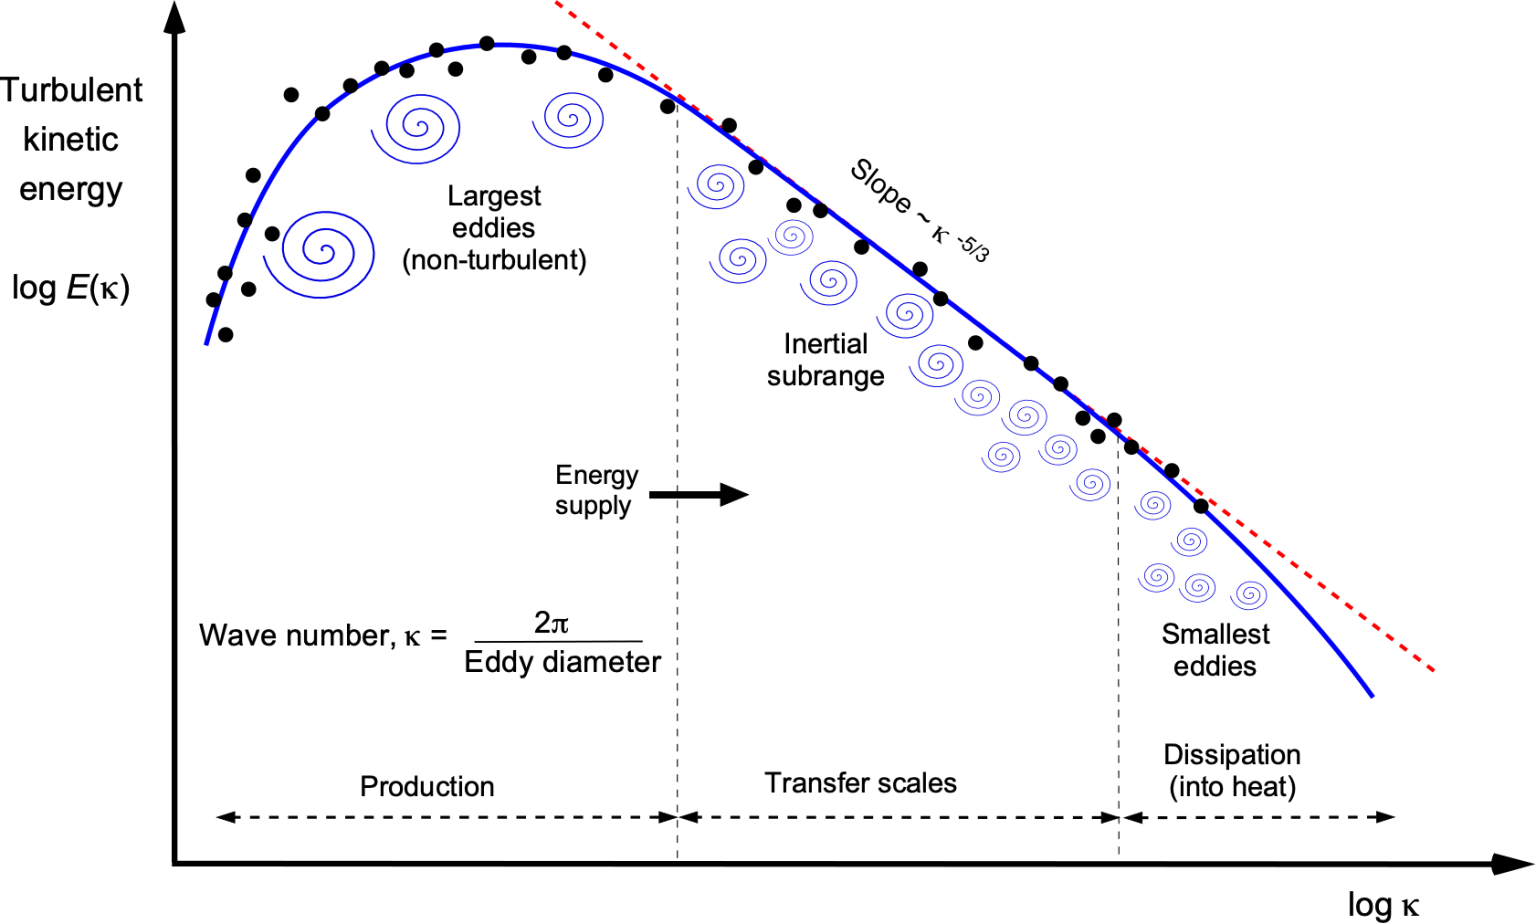
\includegraphics[width=0.9\linewidth]{Intro_img/chapter1_turbulence_spectrum.png}
    \caption[Schematic of a turbulent kinetic energy power spectrum.]{Schematic of a turbulent kinetic energy power spectrum. Reproduced from
    \citet{leishman_introduction_2026}, Chapter 27, Figure 9.}
    \label{fig:turbulence-spectrum}
\end{figure}

\subsection{Effects of compressibility and Mach number on turbulence}

Turbulence can stir a fluid to a characteristic velocity fluctuation, $v_{\rm turb}$. 
Here, the sonic Mach number, $M$, determines the properties of the turbulent flow:
\begin{equation}
    M = \frac{v_{\rm turb}}{c_s},
\end{equation}
where $c_s$\ is the sound speed of the fluid. 
At $M \lesssim 0.3$, pressure waves can smooth out density contrasts and the flow remains close to an incompressible fluid \citep{leishman_introduction_2026}, following the Kolmogorov cascade.
As the flow becomes supersonic ($M \gtrsim 1$), density waves cannot propagate fast enough to smooth out the flow. 
Supersonic turbulence thus introduces shocks that affect the velocity statistics, steepening the kinetic energy spectrum to $E(k) \propto k^{-2}$ \citep[Burgers turbulence,][]{burgers_mathematical_1995,federrath_universality_2013}.

Subsonic, incompressible turbulence is often a good approximation for planetary processes, such as atmospheric disturbances and ocean currents.
Astrophysical environments, however, are often better described by supersonic turbulence.
For example, strong turbulence is seen in multiple galaxy clusters as density contrasts along shock fronts \citep{russell_shock_2012,zhuravleva_turbulent_2014}, while ALMA observations of N159E filamentary CO emission show evidence of compressive turbulence \citep{sharda_first_2022}, and radial velocity fluctuations are seen in multiple \ion{H}{2} regions of the Milky Way and other Local Group galaxies \citep{garcia-vazquez_turbulence_2023}.

\subsection{Effects of magnetic fields and intermittency on turbulence}

Beyond compressibility, astrophysical turbulence can also be shaped by additional physics, especially magnetic forces.
In astrophysical plasmas, magnetic fields are dynamically coupled to the fluid through the Lorentz force, so turbulence not only transfers kinetic energy across scales, but also contributes to twisting magnetic field lines, which in turn converts kinetic energy to magnetic energy \citep[e.g.,][]{biskamp_magnetohydrodynamic_2003, beresnyak_mhd_2019}.
In magnetohydrodynamic (MHD) turbulence, two numbers control the characteristics of the flow: the Alfv\'en Mach number, $M_{\rm A}$, and the plasma $\beta$:
\begin{equation}
    M_{\rm A} = \frac{v_{\rm turb}}{v_{\rm A}},
\end{equation}
where $v_{\rm A} = B/\sqrt{4\pi \rho}$\ is the Alfv\'en speed.
The Alfv\'en Mach number measures whether the magnetic field strongly guides the turbulent cascade ($M_{\rm A} < 1$) or if turbulent motions can twist the field more easily ($M_{\rm A} > 1$).
\begin{equation}
    \beta = \frac{P_{\rm gas}}{P_{\rm mag}},
\end{equation}
which is the ratio between thermal pressure and magnetic pressure.
The plasma $\beta$\ parameter indicates how strongly the magnetic field affects the properties of turbulence in a fluid.

Importantly, magnetic fields introduce \textit{anisotropy} to a turbulent velocity field, breaking the isotropic assumption of Kolmogorov turbulence. 
In the strong MHD regime, energy transfers more efficiently perpendicular to the local magnetic field than parallel to it, producing elongated eddies, while the perpendicular kinetic energy spectrum remains Kolmogorov-like, $E(k_{\perp}) \propto k_{\perp}^{-5/3}$ \citep{goldreich_toward_1995}.
For example, in situ measurements of the fast solar wind show anisotropic magnetic-field fluctuations with different spectral scalings parallel and perpendicular to the local field \citep{wicks_power_2010}, while Galactic \ion{H}{1} observations reveal long, magnetically aligned fibers that trace the projected interstellar magnetic field \citep{clark_magnetically_2014}.

Another important characteristic of MHD turbulence, especially at small scales, is intermittency. 
Intermittency is the tendency of a turbulent flow not to follow a statistically uniform distribution, but instead to become increasingly sparse in time or space with decreasing scale size \citep{biskamp_magnetohydrodynamic_2003}.
In magnetized plasma turbulence, intermittency manifests as current sheets; this manifestation is discussed in more detail in Chapter~\ref{chap:ml}.
Figure~\ref{fig:turbulence-regimes} illustrates these characteristics across four examples of astrophysical turbulence modified by strong shocks \citep{russell_shock_2012}, supersonic driving \citep{federrath_universality_2013}, \ion{H}{2} ionization \citep{medina_turbulence_2014}, and intermittency \citep{dong_reconnection-driven_2022}.

\begin{figure}
    \centering
    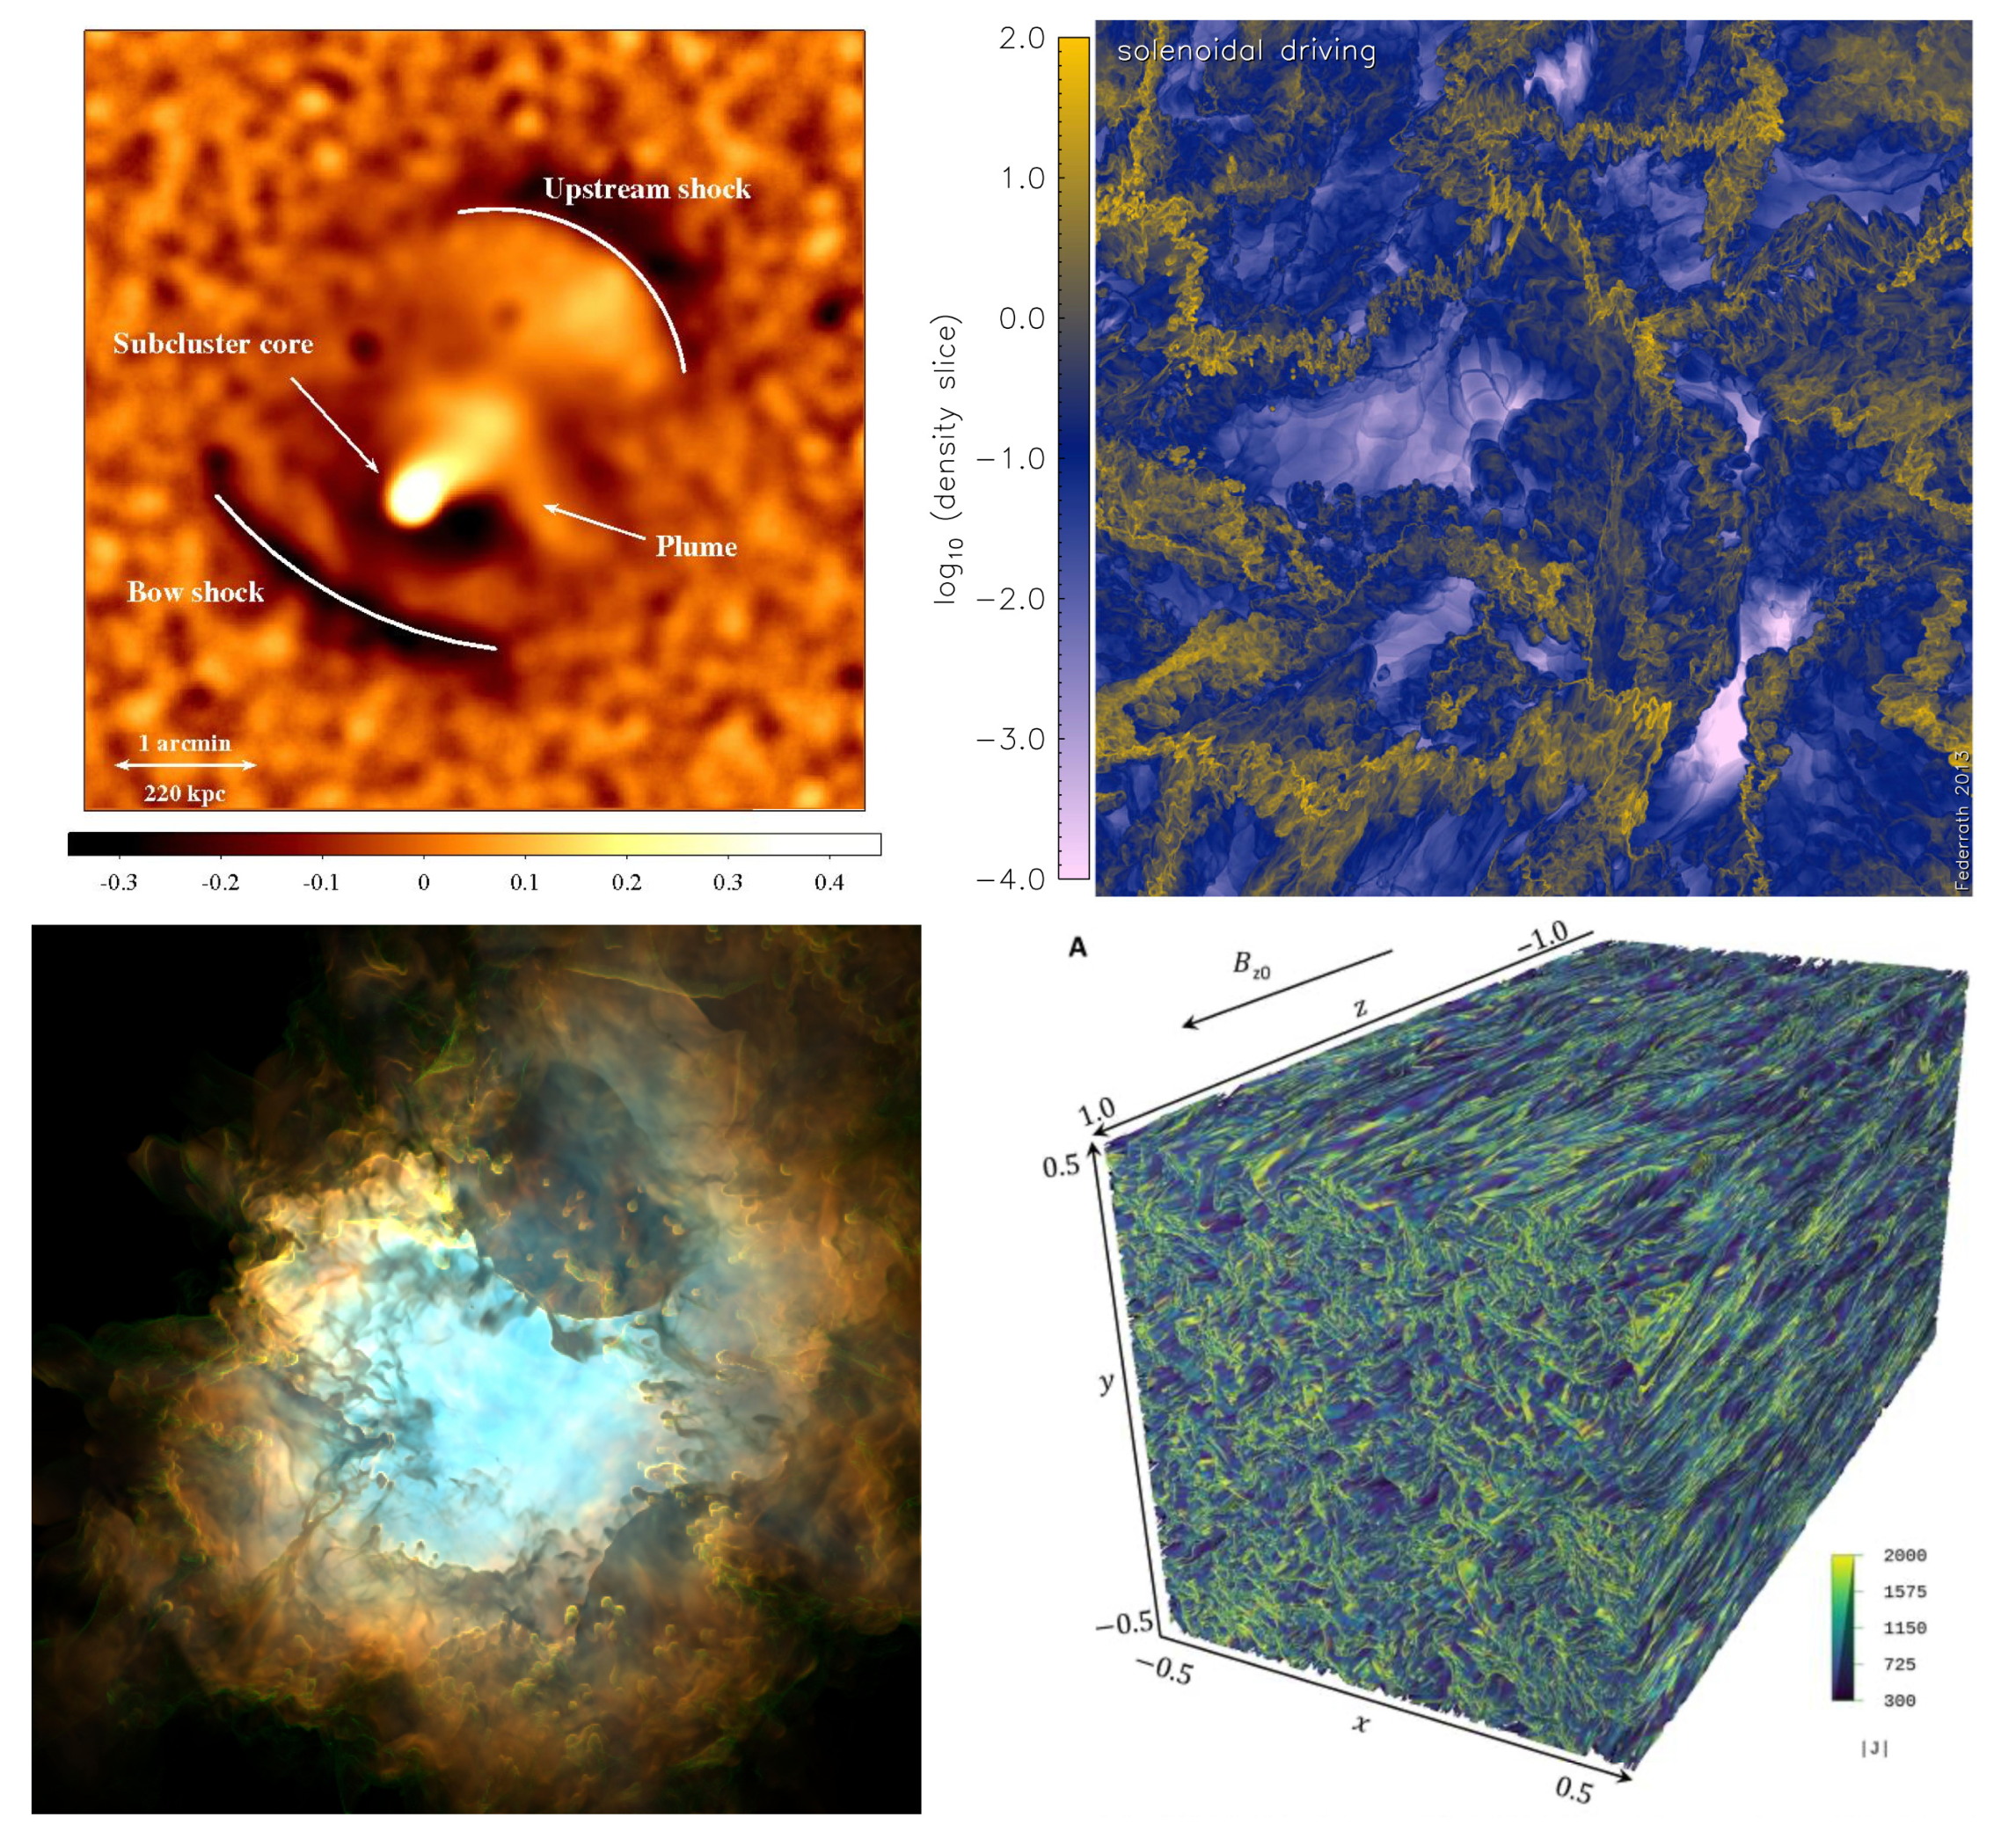
\includegraphics[width=\linewidth]{Intro_img/chapter1_turbulence_regimes.pdf}
    \caption{Representative examples of astrophysical turbulence beyond the Kolmogorov model. Top left: shock fronts observed in galaxy cluster Abell 2146, caused by a merger. Adapted from \citet{russell_shock_2012}. Top right: a slice of a solenoidally driven turbulence simulation, with structure similar to that found in the ISM\@. Adapted from \citet{federrath_universality_2013}. Bottom left: simulated projected image of an evolving \ion{H}{2} region in a turbulent molecular cloud. Adapted from \citet{medina_turbulence_2014}. Bottom right: volume rendering of current density in fully developed MHD turbulence. Adapted from \citet{dong_reconnection-driven_2022}.}
    \label{fig:turbulence-regimes}
\end{figure}

\section{The Three Regimes of Astrophysical Turbulence in This Dissertation}

\begin{table}[t]
\centering
\caption{Three regimes of turbulence and diagnostic tools studied in this dissertation.}
\label{tab:intro-regimes}
\renewcommand{\arraystretch}{1.25}
\begin{tabular}{@{}>{\raggedright\arraybackslash}p{0.24\textwidth}>{\raggedright\arraybackslash}p{0.68\textwidth}@{}}
\toprule
Regime & Physical setting and diagnostic approach \\
\midrule
Active galactic nucleus (AGN) atmospheres &
Scale: $10^4$--$10^6\ \mathrm{pc}$\newline
Main drivers: SMBH jet feedback in low-accretion-rate systems\newline
Main limitation: unresolved accretion physics\newline
Diagnostic: hydrodynamic multi-scale simulations \\
ISM and molecular clouds &
Scale: $10^0$--$10^4\ \mathrm{pc}$\newline
Main drivers: stellar outflows, SNe, and galactic shear\newline
Main limitation: projection and tracer bias\newline
Diagnostic: velocity statistics from young stars \\
Relativistic plasma &
Scale: $10^{-4}$--$10^{-1}\ \mathrm{pc}$\newline
Main driver: magnetic-field fluctuations\newline
Main limitation: inefficient identification of intermittent structures in large datasets\newline
Diagnostic: machine-learning segmentation \\
\bottomrule
\end{tabular}
\end{table}

Astrophysical turbulence plays an important role in shaping gas morphology across vast spatial scales.
This dissertation focuses on three representative regimes across that large dynamical range (see Table~\ref{tab:intro-regimes} for a summary):
\begin{enumerate}
    \item $10\ \mathrm{kpc} \lesssim \ell \lesssim 1\ \mathrm{Mpc}$: in the circumgalactic medium (CGM) at the outskirts of galaxies and in the ICM, SMBH feedback injects vast amounts of energy ($\dot{E} \approx 10^{42}\text{--}10^{45}\ \mathrm{erg\ s^{-1}}$) into the surrounding medium, helping to balance the overall radiative cooling of the X-ray-emitting atmosphere \citep{fabian_cooling_1994}. In low-luminosity systems such as M87, this feedback is dominated by relativistic jets \citep{fabian_observational_2012,li_direct_2020}, while high-accretion-rate systems can also drive accretion-disk winds and radiative outflows \citep[][]{murray_accretion_1995}.
    \item $1\ \mathrm{pc} \lesssim \ell \lesssim 10\ \mathrm{kpc}$: inside the ISM, cold and dense molecular clouds collapse under self-gravity to form stars.
    Various stellar processes such as winds and SNe drive turbulence on pc scales and regulate the star formation process \citep[][]{mac_low_control_2004,mckee_theory_2007,hennebelle_turbulent_2012}.
    Galactic shear and other large-scale processes also drive turbulence in this regime \citep[e.g.,][]{piontek_models_2007,forbes_gas_2023}.
    \item $10^{-4}\ \mathrm{pc} \lesssim \ell \lesssim 0.1\ \mathrm{pc}$: in extremely high-energy environments near rapidly accreting neutron stars and black holes, at scales comparable to the object's gravitational radius, the flows are accompanied by strong magnetic-field fluctuations \citep{biskamp_magnetohydrodynamic_2003, beresnyak_mhd_2019}.
    The non-linear interactions between the magnetic field and local plasma produce violent energy dissipation events observed in gamma-ray bursts \citep[e.g.,][]{beniamini_prompt_2017,lazarian_gamma-ray_2019}.
\end{enumerate}

\section{Limitations of Existing Techniques in Measuring Turbulence}

Astrophysical turbulence is notoriously difficult to measure. 
Turbulence is multi-dimensional and time-dependent, yet the tools we possess to probe it predominantly offer an incomplete picture of the flow.
Spectral observations can only probe the line-of-sight (LOS) velocity and the plane-of-the-sky position, leaving unresolved projection uncertainties.
Spatially, turbulence can span many orders of magnitude (see the previous section for examples of the length scales involved), but current instruments are resolution-limited and can only probe parts of a turbulent cascade \citep[e.g.,][]{hitomi_collaboration_atmospheric_2018,churazov_x-ray_2012}.
Observations of turbulence are also limited by the choice of tracer, since turbulence manifests differently in different phases of gas. 
For example, the ISM contains both cold molecular gas ($T \approx 10^2\ \mathrm{K}$) and warm ionized gas ($T \approx 10^4\ \mathrm{K}$). 
Studies have suggested that most of the kinetic energy injected by SNe is deposited into low-density regions of the ISM \citep[see, e.g.,][]{kim_momentum_2015,padoan_supernova_2016}, driving significant turbulence in the warm ionized gas while leaving the molecular phase comparatively less perturbed.
Therefore, no single observational campaign can recover the full velocity field and energy cascade of a turbulent system.

The problem becomes even more pronounced in time.
The turbulent timescales in the molecular ISM are on the order of $10^6$--$10^7$ years \citep{sun_molecular_2022}, and ICM turbulent timescales are even longer, $\sim 10^8$--$10^9$ years \citep{hitomi_collaboration_atmospheric_2018}. 
Meanwhile, the longest survey conducted to study how turbulence evolves in the solar wind has only been collecting data for the past $\sim 30$\ years \citep{wilson_quarter_2021}.
In essence, observations only provide snapshots of complex environments where the turbulent cascade and its driving processes coexist and are difficult to untangle.

Since the turn of the century, advances in numerical methods and computational capabilities have enabled a different kind of turbulence modeling.
Currently, two numerical treatments are commonly used to model astrophysical turbulence.
At the galaxy scale, MHD simulations discretize fluid variables onto grid cells, making it possible to follow gas, magnetic fields, gravity, cooling, and feedback over large volumes \citep[e.g.,][]{somerville_physical_2015,beresnyak_mhd_2019}.
In systems where Lorentz-force coupling is important, such as magnetic reconnection near compact objects, relativistic jets, or pulsar winds, particle-in-cell simulations are often the preferred treatment because they evolve charged particles and electromagnetic fields together \citep[e.g.,][]{zweibel_magnetic_2009,kagan_relativistic_2015}.
These simulations give us access to time evolution of turbulence that observations cannot provide, but other challenges remain.
Galaxy simulations cannot resolve dissipation scales, while particle-in-cell simulations resolve kinetic physics only in domains far smaller than the astrophysical systems they represent.
Running such calculations is also expensive, so modern simulations remain approximations of real environments rather than complete reconstructions.
To understand the full picture of turbulence from global driving to local dissipation, next-generation multi-scale methods are needed to bridge this gap.

\section{Introducing the Next Generation of Diagnostic Tools for Turbulent Systems}

This dissertation brings together six years of research on the nature of turbulence in the three physical regimes introduced above.
Specifically, I developed and applied \textit{diagnostic tools}: statistical, machine-learning, and simulation frameworks that turn incomplete data into physical constraints on a turbulent system.
The first diagnostic tool uses young stars as tracers of the turbulent velocity field in their natal molecular clouds.
In Chapter~\ref{chap:stars}, I introduce this method through two first-author studies: a proof-of-concept application to the Orion Complex, where stellar kinematics reveal a signature of the turbulent cascade \citep{ha_measuring_2021}, and a broader comparison across Ophiuchus, Perseus, and Taurus, where stellar velocity statistics are benchmarked against gas kinematic measurements \citep{ha_turbulence_2022}.
Together, these studies established the conditions under which young stars can preserve information about molecular-cloud turbulence, how subsequent dynamical evolution contaminates this information, and how multi-tracer measurements can distinguish between different drivers of turbulence in star-forming environments.

The second diagnostic tool applies machine learning to intermittent structures in relativistic plasma turbulence.
In Chapter~\ref{chap:ml}, I introduce \awesom, a theory-agnostic clustering package based on self-organizing maps and ensemble learning that I developed to identify complex structures in large simulation datasets \citep{ha_awesom_2025}.
I then apply \awesom\ to three-dimensional plasma simulations, showing that machine-learning methods can identify current sheets with high accuracy and separate them into distinct ``single current sheet'' and ``double current sheet'' morphologies \citep{ha_machine_2025}.
These morphologies form under different physical conditions and may dissipate energy at different rates, making them important targets for future subgrid treatments of plasma turbulence.

The third diagnostic tool uses hydrodynamic simulations to study turbulent multiphase accretion flows onto SMBHs.
In Chapter~\ref{chap:sim}, I describe a suite of simulations from an upcoming first-author study, \citet{ha_galaxy-_2026}, that probes low-luminosity AGN accretion, the limits of the Bondi accretion model, and resolution effects that shape the morphology of cool gas.
This simulation-based diagnostic complements the statistical and machine-learning tools developed in the previous chapters by using controlled numerical experiments to connect unresolved accretion physics with observable multiphase structure.

\section{Related Works}

As a graduate researcher, I had the pleasure of contributing to several research projects that concluded in peer-reviewed publications. 
Although these publications are not highlighted in the main body of this dissertation, they coincide with the overarching goal of my doctoral work: to develop statistical and machine-learning tools that advance our ability to measure astrophysical turbulence and that can be reused and extended by future studies. 

\subsection{As Contributing Author}

I was the third author of \citet{velguth_probing_2025}, which extends the analyses from my early works \citep{ha_measuring_2021, ha_turbulence_2022}.
It is a natural generalization of the young-star turbulence framework: rather than treating the stellar velocity structure function (VSF) only as a measurement of inherited molecular-cloud turbulence, we used the same diagnostic to ask how that initial turbulent imprint is modified by subsequent dynamical evolution and environmental effects (e.g., from gravity, SNe, Galactic shear, and magnetic fields). 
I was directly involved in mentoring the first author, a post-baccalaureate fellow, during the early months of the project, helping to frame the scientific question, interpret the VSF results, and connect the analysis to the methodology developed in Chapter~\ref{chap:stars}.

I was also the third author of \citet{reinheimer_black_2025}, which introduces machine-learning regression to model SMBH--host galaxy relationships. 
Previously, these relationships were modeled by linear fits to a single feature ($\sigma$, $M_{\star}$, $M_{\rm halo}$), which introduced large uncertainties at low SMBH mass. 
We found that several machine-learning regression algorithms, such as XGBoost and multi-layer perceptrons, could provide better predictions of the SMBH mass throughout the mass range, suggesting that these algorithms are better at handling the intrinsic non-linearity of astrophysical systems.
Furthermore, combining multiple host-galaxy properties produced more accurate SMBH mass predictions than any individual one-dimensional scaling relation.
This work, together with the algorithm that I detail in Chapter~\ref{chap:ml}, highlights how machine-learning methods can evolve beyond curve fitting or classification alone to reveal physically meaningful structure in large, complex astrophysical datasets.

\subsection{As First Author}

I was the first author on one other project during this period, which addressed a related problem in observational quasar accretion physics. 
In \citet{ha_shedding_2023}, I studied weak emission-line quasars (WLQs), a subset of type 1 quasars with unusually weak rest-frame ultraviolet (UV) emission lines, and investigated how their emission-line properties connect to black-hole accretion rates. 
By comparing WLQs with ordinary quasars in the \ion{C}{4} equivalent-width--blueshift parameter space, I showed that traditional broad-line-region size--luminosity empirical relations can overestimate WLQ black-hole masses by up to an order of magnitude without a correction to the optical \ion{Fe}{2} emission.
I then used the corrected Eddington luminosity ratios (a proxy of black hole accretion rates) to find a significant correlation with a multi-dimensional \ion{C}{4} spectral feature across both WLQs and ordinary quasars.
From this result, we concluded that WLQs are not outliers compared to other type 1 quasars, but instead are preferentially situated at the tail of a multi-dimensional UV distribution without being statistically out of distribution. 
% Although this work falls outside the main turbulence-focused structure of the dissertation, it reflects the same broader interest in using imperfect observational signals to infer the physical state of accreting SMBHs, a topic I address in Chapter~\ref{chap:sim}.
Although this work falls outside the main turbulence-focused structure of the dissertation, it addresses a similar question about the physical state of accreting SMBHs, which I revisit through simulation in Chapter~\ref{chap:sim}.

\section{Dissertation Outline}

The following chapters detail three research projects I have led during my doctoral work, each focused on a different diagnostic approach to astrophysical turbulence. In Chapter~\ref{chap:stars}, I present young-star velocity statistics as a tracer of turbulence in star-forming molecular clouds. In Chapter~\ref{chap:ml}, I develop and apply machine-learning methods to identify intermittent current sheets in relativistic plasma simulations. In Chapter~\ref{chap:sim}, I use hydrodynamic simulations to study turbulent multiphase accretion flows onto SMBHs. Finally, Chapter~\ref{chap:summary} summarizes the dissertation and outlines future work.

\chapter{\texorpdfstring{\MakeUppercase{Measuring Turbulence in the Interstellar Medium with Young Stars}}{Measuring Turbulence in the Interstellar Medium with Young Stars}}
\label{chap:stars}


\begin{figure}[b]
    \centering
    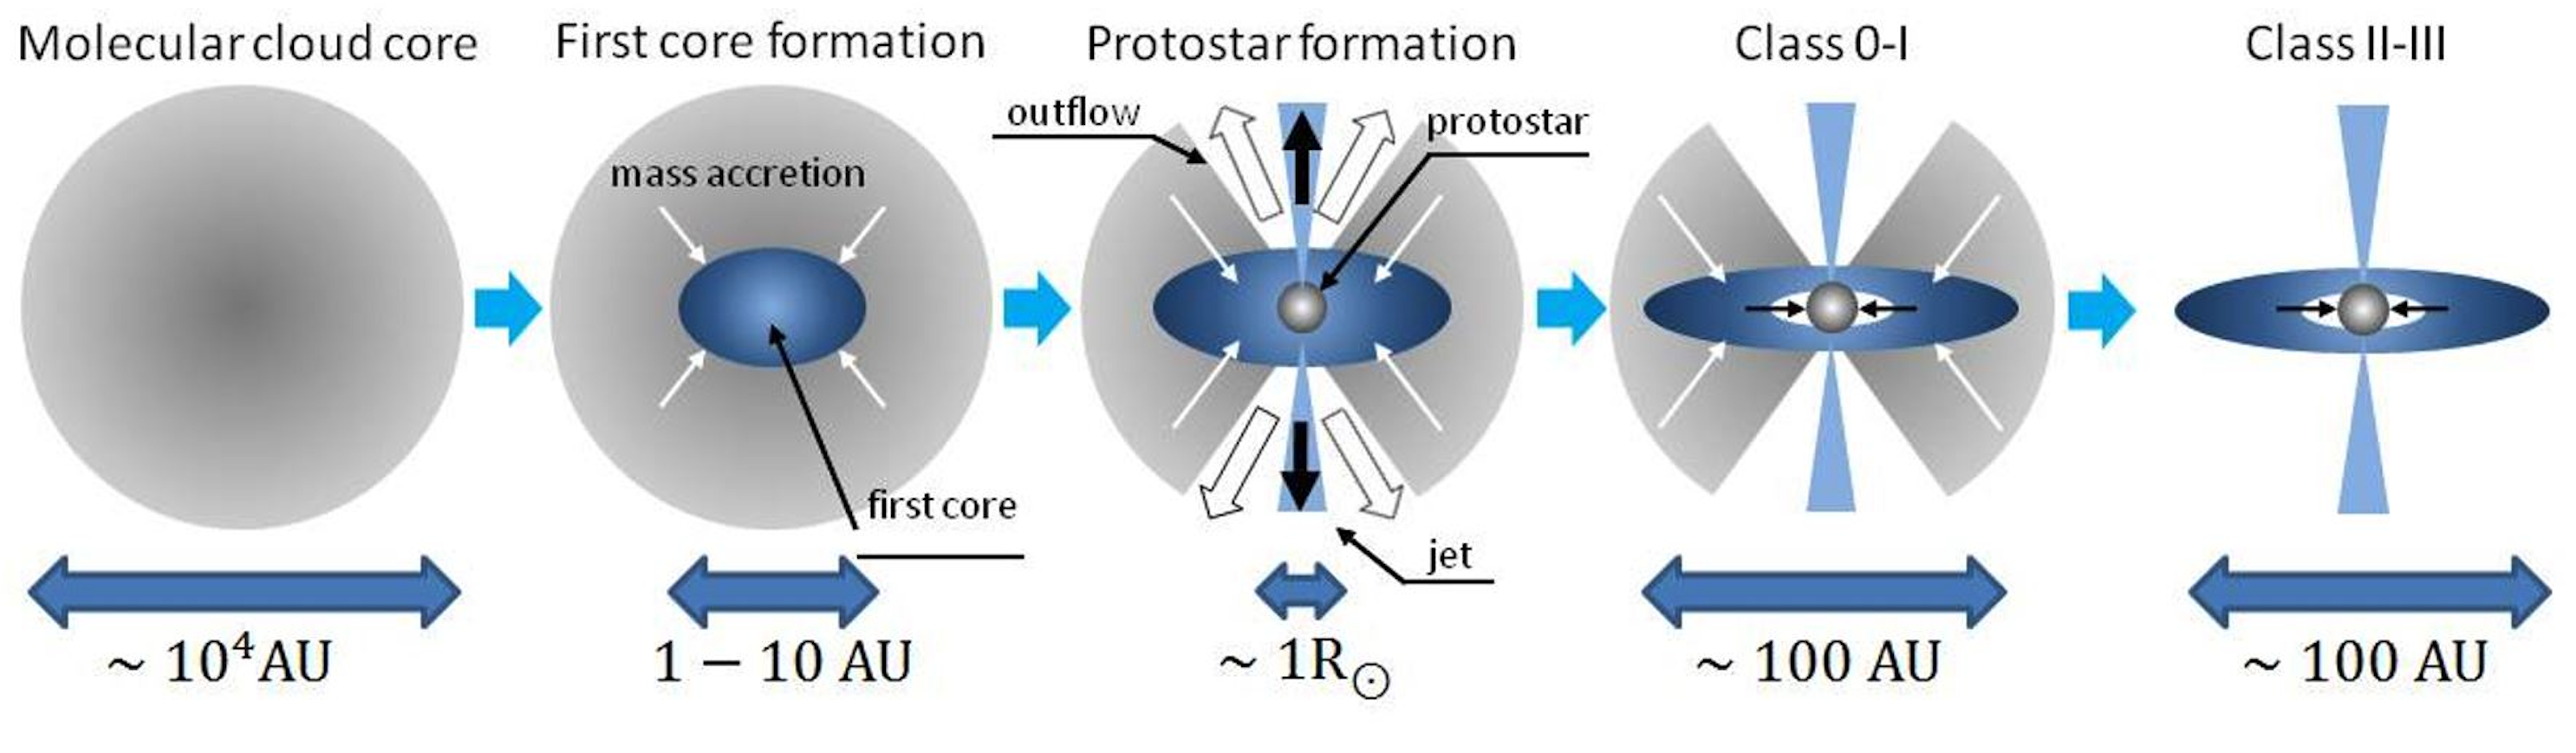
\includegraphics[width=0.8\linewidth]{Stars_img/star_formation_illustration.png}
    \caption[Illustration of the star formation process.]{Illustration of the star formation process. Credit: Yusuke Tsukamoto, RIKEN.}
    \label{fig:star-formation}
\end{figure}

Inside the interstellar medium (ISM), molecular clouds are sites of star formation.
The densest parts of these clouds, the \textit{molecular cores}, undergo gravitational collapse to form stars (see Figure~\ref{fig:star-formation}). 
It is well known that the ISM is multiphase and turbulent \citep{mckee_theory_2007}.
\cite{larson_turbulence_1981} investigated the kinematic properties of various molecular clouds within the Milky Way, and found a power-law relation between the velocity dispersion and cloud size, indicative of a Kolmogorov-like turbulent cascade in the local universe. 
Previously, turbulence in the ISM has been detected and analyzed using a variety of gas tracers.
The warm-ionized phase can be probed with \halpha\ \citep{haffner_wisconsin_2003}, the warm-neutral medium with \ion{H}{1} \citep[e.g.,][]{burkhart_characterizing_2009}, the cold molecular phase with CO, HCO, NH$_3$, etc. \citep[e.g.,][]{turner_physics_1997,qian_13co_2012,heyer_universality_2004}.
In these studies, the line-of-sight velocities at individual angular positions are measured by computing the Doppler shift of the emission/absorption line.
These tracers provide extremely reliable measurements, but fail to describe a complete picture of the local velocity field, lacking one spatial dimension and two velocity dimensions.
Thus, measurements of turbulence often suffer from projection effects that are difficult to correct for \citep{qian_new_2015}.

In \citet[][]{ha_measuring_2021} and \citet[][]{ha_turbulence_2022}, we proposed a new method to probe turbulence in star-forming regions of the Milky Way.
Since stars form out of turbulent molecular cores, we hypothesized that the newly born stars could \textit{inherit} the turbulent kinematics of their natal clouds.
To test this theory, we utilized six-dimensional (6D) kinematic measurements of young stars in Orion \citep{ha_measuring_2021}, Ophiuchus, Perseus, and Taurus \citep{ha_turbulence_2022} from the Gaia \citep{collaboration_gaia_2016,brown_gaia_2021} and APOGEE-2 \citep{blanton_sloan_2017} surveys.
If young stars were good tracers of turbulence in the ISM, we predicted that the usual characteristics of turbulence (i.e., a statistically coherent motion) would also be seen in their astrometries.
This procedure also gave us access to a complete kinematic picture of young stars in these regions, bypassing limitations imposed by projection effects.

In the following studies, we measured the level of turbulence in each region using a technique called the velocity structure function (VSF).
The VSF is related to the kinetic energy power spectrum of a velocity field, and is expressed as a two-point correlation function relating the absolute velocity differences $|\delta v|$ to the physical separation $\ell$. For a turbulent velocity field, the VSF follows a characteristic power-law scaling, $|\delta v| \propto \ell^k$, with slope $k = 1/3$ for incompressible turbulence dominated by solenoidal motions \citep[][]{kolmogorov_local_1941}, or a slope $k = 1/2$ for supersonic turbulence dominated by compressive motions \citep{burgers_mathematical_1995}. For the Milky Way molecular clouds, \citet{larson_turbulence_1981} found a relationship between cloud size and velocity dispersion to be $\sigma = 1.1~R^{0.38}$.

The following sections are adapted from \citet{ha_measuring_2021}, the Astrophysical Journal Letters, 907, L40, and \citet{ha_turbulence_2022}, the Astrophysical Journal, 934, 7.

\section{The Signal of Turbulence from Young Stars in the Orion Complex}

\publicationdetails
{Ha et al. 2021, ApJL, 907, L40}
{Trung Ha\footnotemark[1], Yuan Li\footnotemark[1]\footnotemark[2], Siyao Xu\footnotemark[3]\footnotemark[7], Marina Kounkel\footnotemark[4], and Hui Li\footnotemark[5]\footnotemark[6]\footnotemark[7]}
{Stars form in molecular clouds in the interstellar medium (ISM) with a turbulent kinematic state. Newborn stars therefore should retain the turbulent kinematics of their natal clouds. Gaia DR2 and APOGEE-2 surveys in combination provide three-dimensional (3D) positions and 3D velocities of young stars in the Orion Molecular Cloud Complex. Using the full 6D measurements, we compute the velocity structure functions (VSFs) of the stars in six different groups within the Orion Complex. We find that the motions of stars in all diffuse groups exhibit strong characteristics of turbulence. Their first-order VSFs have a power-law exponent ranging from $\sim0.2$--$0.5$ on scales of a few to a few tens of parsecs, generally consistent with Larson's relation. On the other hand, dense star clusters, such as the Orion Nebula Cluster (ONC), have experienced rapid dynamical relaxation, and have lost the memory of the initial turbulent kinematics. The VSFs of several individual groups and the whole Complex all show features supporting local energy injection from supernovae. The measured strength of turbulence depends on the location relative to the supernova epicenters and the formation history of the groups. Our detection of turbulence traced by young stars introduces a new method of probing the turbulent kinematics of the ISM\@. Unlike previous gas-based studies with only projected measurements accessible to observations, we utilize the full 6D information of stars, presenting a more complete picture of the 3D interstellar turbulence.}
{\footnotetext[1]{Department of Physics, University of North Texas, Denton, TX 76203, USA}
\footnotetext[2]{Department of Astronomy, University of California, Berkeley, CA 94720, USA}
\footnotetext[3]{Institute for Advanced Study, 1 Einstein Drive, Princeton, NJ 08540, USA}
\footnotetext[4]{Department of Physics and Astronomy, Western Washington University, 516 High St, Bellingham, WA 98225, USA}
\footnotetext[5]{Department of Physics, Kavli Institute for Astrophysics and Space Research, Massachusetts Institute of Technology, Cambridge, MA 02139, USA}
\footnotetext[6]{Department of Astronomy, Columbia University, 550 West 120th Street, New York, NY 10027, USA}
\footnotetext[7]{NASA Hubble Fellow}}

\subsection{Introduction}
\label{sec:orion-intro} 
\setcounter{footnote}{0} 
The interstellar medium (ISM) is turbulent. More specifically, the cold dense star-forming molecular clouds are turbulent. For example, \citet{larson_turbulence_1981} finds a power law relation between velocity dispersion and cloud size with an exponent of 0.38, similar to the Kolmogorov law for incompressible turbulence \citep{kolmogorov_local_1941}. Turbulence plays an important role in regulating the cloud dynamics and star formation \citep{mac_low_control_2004, mckee_theory_2007,hennebelle_turbulent_2012},
from cloud scales all the way down to the scales much smaller than molecular cores 
\citep{hull_unveiling_2017}.

The ubiquitous interstellar turbulence induces velocity fluctuations on all scales in both diffuse interstellar phases and dense star-forming gas. Statistical measurements of velocity fluctuations in the multiphase ISM can be done using the Velocity Channel Analysis (VCA), the Velocity Coordinate Spectrum (VCS) \citep{lazarian_velocity_2000,lazarian_studying_2006}, the Delta-variance technique \citep{ stutzki_fractal_1998,ossenkopf_turbulent_2002}, or the Principal Component Analysis \citep{ heyer_universality_2004,roman-duval_turbulence_2011} based on spectroscopic data.
These analyses generally reveal power-law spectra of turbulent velocities \citep{ lazarian_obtaining_2009,chepurnov_velocity_2010}.

Many processes can drive turbulence in the ISM, such as gravity, shear, and various forms of stellar feedback including supernova explosions \citep{krumholz_is_2016,padoan_supernova_2016}. Turbulent motions shape the filamentary density structures in molecular clouds (e.g., \citealt{ federrath_universality_2016,xu_formation_2019}). Dense cores and protostars subsequently form in dense filaments \citep{andre_interstellar_2017}.

Besides gas tracers that are commonly used to probe turbulence in the 
volume filling ISM, 
turbulent velocities can also be sampled using point sources 
such as molecular cores formed at the density peaks generated in highly supersonic turbulence. 
For example, \citet{qian_13co_2012} developed statistical measurements of 
core-to-core velocity dispersion over a range of length scales, i.e.,
the core velocity dispersion technique. \citet{qian_studies_2018} find 
signatures for a turbulent power-law spectrum in the Taurus Molecular Cloud, and demonstrate that the statistics of turbulent velocities are imprinted in the velocities of dense cores \citep{xu_projected_2020}. 

Because prestellar cores are nurseries of stars, newborn stars should naturally inherit the velocities of cores and hold the fossil information on the turbulent velocities of their natal clouds, as long as dynamical interactions of young stars have not erased that information.

In this work, we carry out the first statistical analysis of star-to-star velocity structure function (VSF) across the Orion complex over a range of length scales, from $\sim200$ pc down to $<1$ pc. These newly formed stars are expected to still ``remember" the local gas kinematics at their birth, and can be used to recover the turbulent motions in the parent cloud. With direct measurements on 3D velocities and 3D positions, the statistical study of turbulent velocities with stars do not suffer from the 
complex convolution between density and velocity and the projection effect as that with the commonly used gas tracers. 

In Section~\ref{sec:data}, we describe the data used in this analysis and how we compute the VSFs. We present the VSF for each group in the Orion complex in Section~\ref{sec:orion-results}, and discuss how the slope and amplitude is related to the location and history of the stellar system. In Section~\ref{sec:discussions}, we discuss the uncertainties and biases of the analysis, and how our method and results compare with previous works on turbulence in the ISM.


\subsection{Data Processing}\label{sec:data}

\begin{figure}
    \centering
    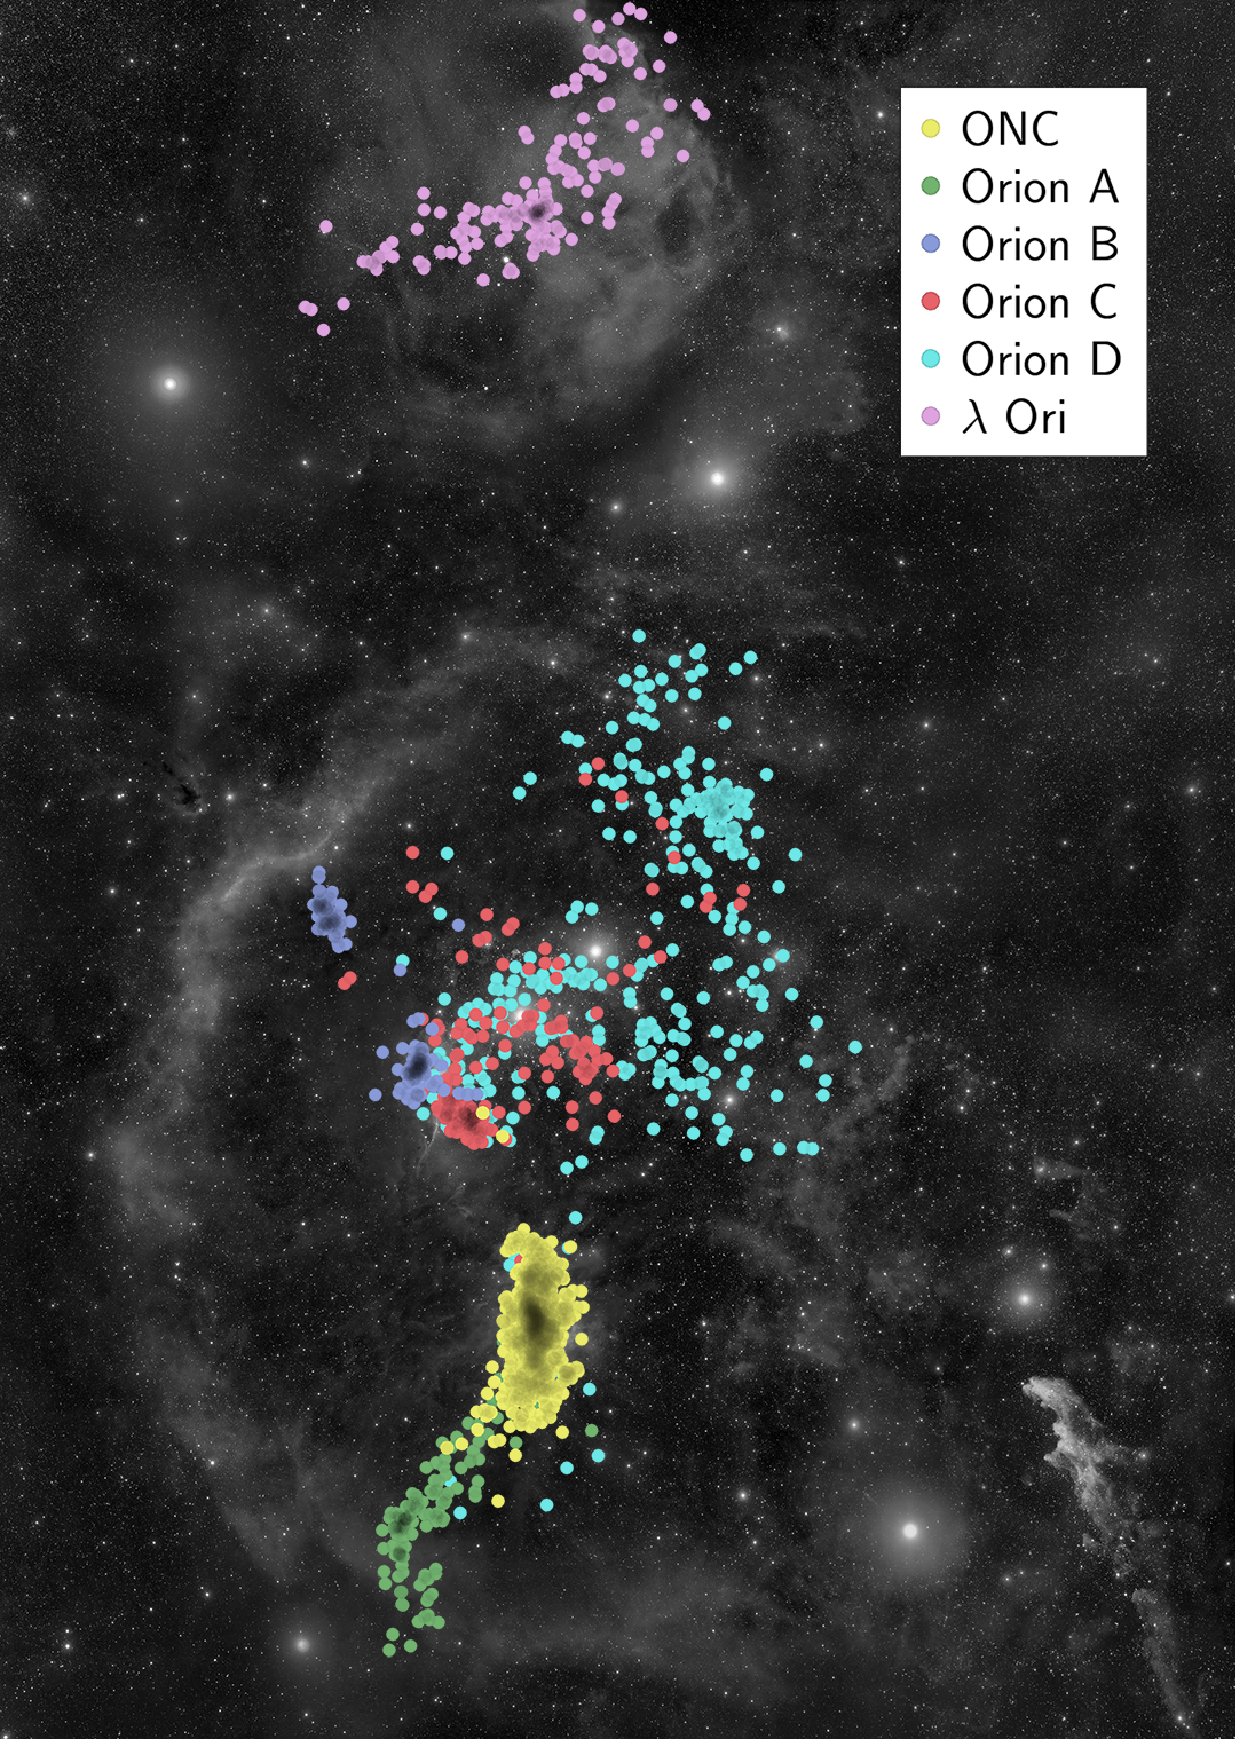
\includegraphics[width=0.8\linewidth]{Stars_img/orion_overlay.pdf}
    \caption{Foreground: each dot represents the projected position of a star in the Orion Complex that we include in our analysis. The star's color corresponds to its main group. Background: greyscale optical image of the Orion Molecular Cloud Complex, courtesy of Rogelio Bernal Andreo.}
    \label{fig:orion}
\end{figure}

\subsubsection{Data Acquisition}\label{sec:data1}
We obtain the locations, parallax distances, and proper motions of stars in the Orion Molecular Cloud Complex from Gaia's second data release \citep{gaia_collaboration_gaia_2018}. The Gaia catalog includes five-parameter astrometric data from over 1.3 billion stars. 
The line-of-sight velocities of the stars were observed in the near infrared during the Apache Point Observatory Galactic Evolution Experiment 2 (APOGEE-2). The APOGEE spectrograph is mounted on the 2.5 m Sloan Foundation Telescope of the Sloan Digital Sky Survey (SDSS), and is used to collect high resolution spectral images of over 400,000 stars in the Milky Way \citep{gunn_25_2006,blanton_sloan_2017}. 
In total, 8891 stars from APOGEE-2, and 16754 stars from Gaia DR2 were observed towards the Orion Complex, as specified by \citet{kounkel_apogee-2_2018}. Combining these two surveys provides six-dimensional information of a subset of stars.

\citet{kounkel_apogee-2_2018} developed a hierarchical clustering algorithm to assess membership of the Orion Complex and its structure based on the position of stars in the phase space (position+velocity). They identify five main groups inside the Complex, namely Orion A, Orion B, Orion C, Orion D, and $\lambda$ Ori. We require all stars in our sample to be a part of one of these groups, excluding all of the stars that could not be clustered together (i.e., field stars, or other members of Orion that may have peculiar velocity---such as spectroscopic binaries or runaways). Furthermore, we require a complete information on six-dimensional position and velocity for each star, i.e., a star needs to have both astrometric solutions from Gaia DR2 as well as radial velocities from APOGEE\@. Through this, we obtain a sample of 1439 stars.

We note that the Orion Nebula Cluster (ONC) is a part of the Orion A molecular cloud, however, it is very unique, being a singularly most massive young cluster in the solar neighborhood. The environment that is found in the ONC is different from the more diffuse environment in the southern part of Orion A. Thus, for the purpose of our analysis, we separate ONC and the rest of the Orion A. Throughout the paper, Orion A refers only to the ``tail'' of the cloud (L1641 and L1647), excluding stars in ONC\@. The reasoning behind this split is discussed in Section~\ref{sec:orion-results}. The term ``group'' in this paper refers to all ``stellar systems'' that are spatially and kinematically associated, while ``cluster'' only refers to open clusters such as the ONC.

Table~\ref{table:data} lists the number of stars and the mean age of each main group and the ONC\@. We plot the projected positions of the stars in our analysis over a greyscale image of the Orion Complex in Figure~\ref{fig:orion}.


\subsubsection{Method of analysis}\label{sec:orion-method}
\begin{figure*}
    \centering
    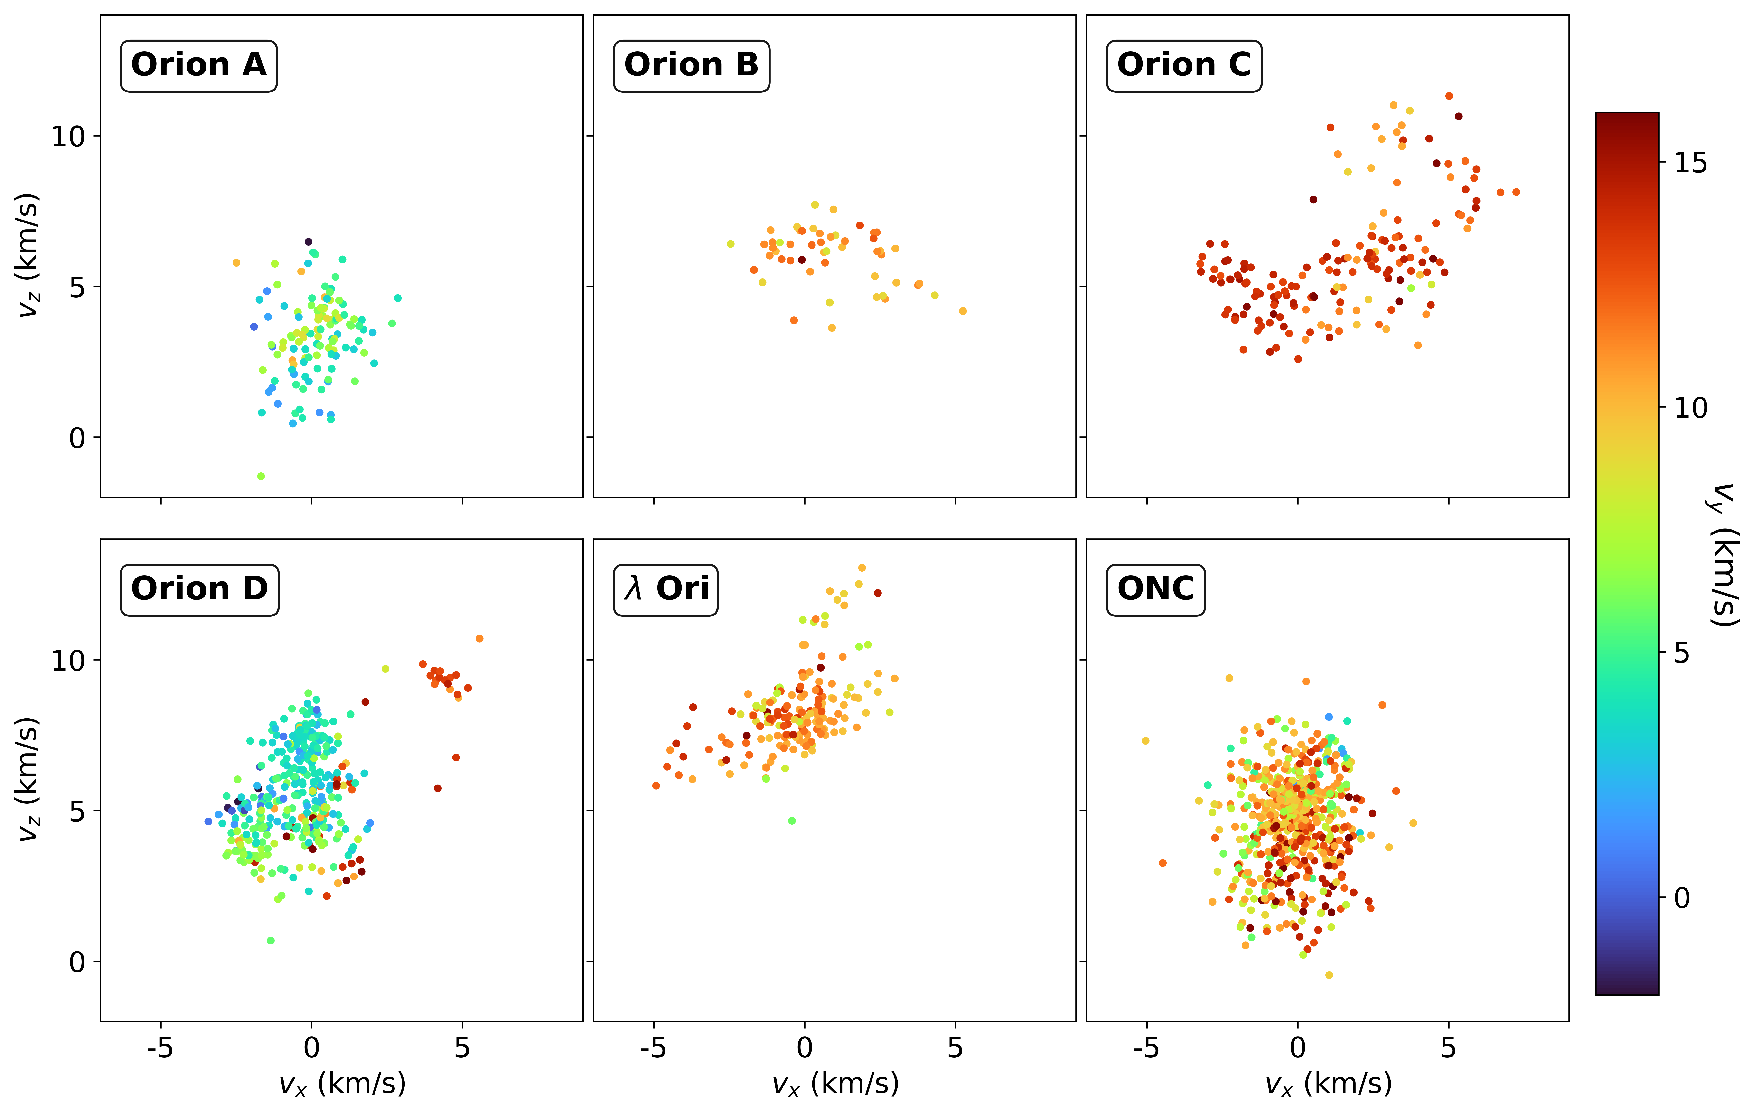
\includegraphics[width=0.98\linewidth]{Stars_img/allVelocities.pdf}
    \caption{Velocities of stars in the six clouds in our analysis in Cartesian coordinate. The color map denotes stars' velocity in the y direction, which closely resembles their radial velocity. All clouds show some level of randomness in the velocities of the stars.}
    \label{fig:velodist}
\end{figure*}
To test our hypothesis that young star clusters ``remember" their local gas kinematics at the time of birth, we compute the VSFs for all identified groups, as well as the VSF of the combined Orion Complex catalog, both with and without the ONC\@. We first convert the radial velocity and proper motion of stars into velocity in Cartesian coordinate, in the Local Standard of Rest (LSR). Figure~\ref{fig:velodist} shows the 3D velocity information of stars used in this study in each cloud.

For each cloud, we compute the first-order VSF and its uncertainties. The VSF for a sample of stars can be calculated in the following way: for each pair of stars, we first record the physical separation $\ell$ of the pair and compute the magnitude of the vector velocity difference $\delta \Vec{v}$ as the velocity difference $|\delta v|$. We then compute the average of the velocity differences $\langle |\delta v| \rangle$ within logarithmic bins of $\ell$. 

The VSF is related to the kinetic energy power spectrum of turbulence. It describes how velocity difference ($|\delta v_{ij}|$) relates to the physical separation ($\ell_{ij}$) for given pairs of points in space ($i$, $j$). In a turbulent flow, kinetic energy cascades down from large scales to small scales, and the velocity differences become smaller toward smaller scales. If the turbulence is incompressible (subsonic), we expect the first-order VSF to be $|\delta v_{ij}|\sim \ell_{ij}^{1/3}$ within the inertial range \citep{kolmogorov_local_1941}. For compressible (supersonic) turbulence, $|\delta v_{ij}|\sim \ell_{ij}^{1/2}$ \citep[e.g.,][]{federrath_universality_2013}.

To estimate uncertainties of the VSF, we first perform random sampling of the measurements of stars' properties based on the observed uncertainties, and obtain 1000 realizations for each star following a Gaussian distribution. We only consider measurement uncertainties of the parallax distances, proper motions, and radial velocities. We ignore the uncertainties in RA and Dec because they are typically much smaller than the uncertainties of other quantities. For each group, we then obtain 1000 VSFs, with each iteration excluding a random star within the group. This allows us to account for both measurement errors and uncertainties due to small sampling sizes in some bins of $\ell$. We take the mean and standard deviation of the computed VSFs to be the group's VSF and its corresponding error. We choose 1000 iterations to ensure accuracy even though the results are already converged at 100 iterations. We also compute the second and third-order VSFs of the groups, and discuss them in Section~\ref{subsec:high_order}.

\begin{sidewaystable}
    \centering
    \caption{Properties of molecular clouds in the Orion Complex}
    \label{table:data}
    \begin{tabular}{ccccccc}
        \toprule
                              & Orion A   & Orion B  & Orion C  & Orion D   & Lambda Ori & ONC      \\
        \midrule
        Number of Stars$^a$   & 117       & 51       & 162      & 354       & 170        & 585      \\
        Median Age (Myr)      & 2.2       & 1.3      & 4.1      & 4.9       & 3.7        & 2.7      \\
        Crossing Time (Myr)   & 16.1      & 13.6     & 8.0      & 12.9      & 12.8       & 6.9$^b$  \\
        Fitting Range$^c$ (pc)& 10--90  & 8--60  & 9--50  & 15--58  & 10--32   & 5--40  \\
        Slope of VSF          & $0.18$    & $0.14$   & $0.19$   & $0.53$    & $0.36$     & $0.05$   \\
        \bottomrule
    \end{tabular}
    \parbox{\linewidth}{\footnotesize \textit{Note.} $^a$ Number of stars obtained 
    from the combined Gaia DR2 and APOGEE surveys with full 6D information 
    (Section~\ref{sec:data1}). $^b$ This is the crossing time for the entire ONC 
    cluster. The inner core has a much shorter crossing time and relaxation time 
    \citep{hillenbrand_preliminary_1998}. $^c$ The slope of the VSFs depends on the exact range 
    of separation taken into account. We choose the fitting range such that the 
    uncertainties are low and there is a consistent trend in the slope of the VSF.}
\end{sidewaystable}


\begin{figure*}
\centering
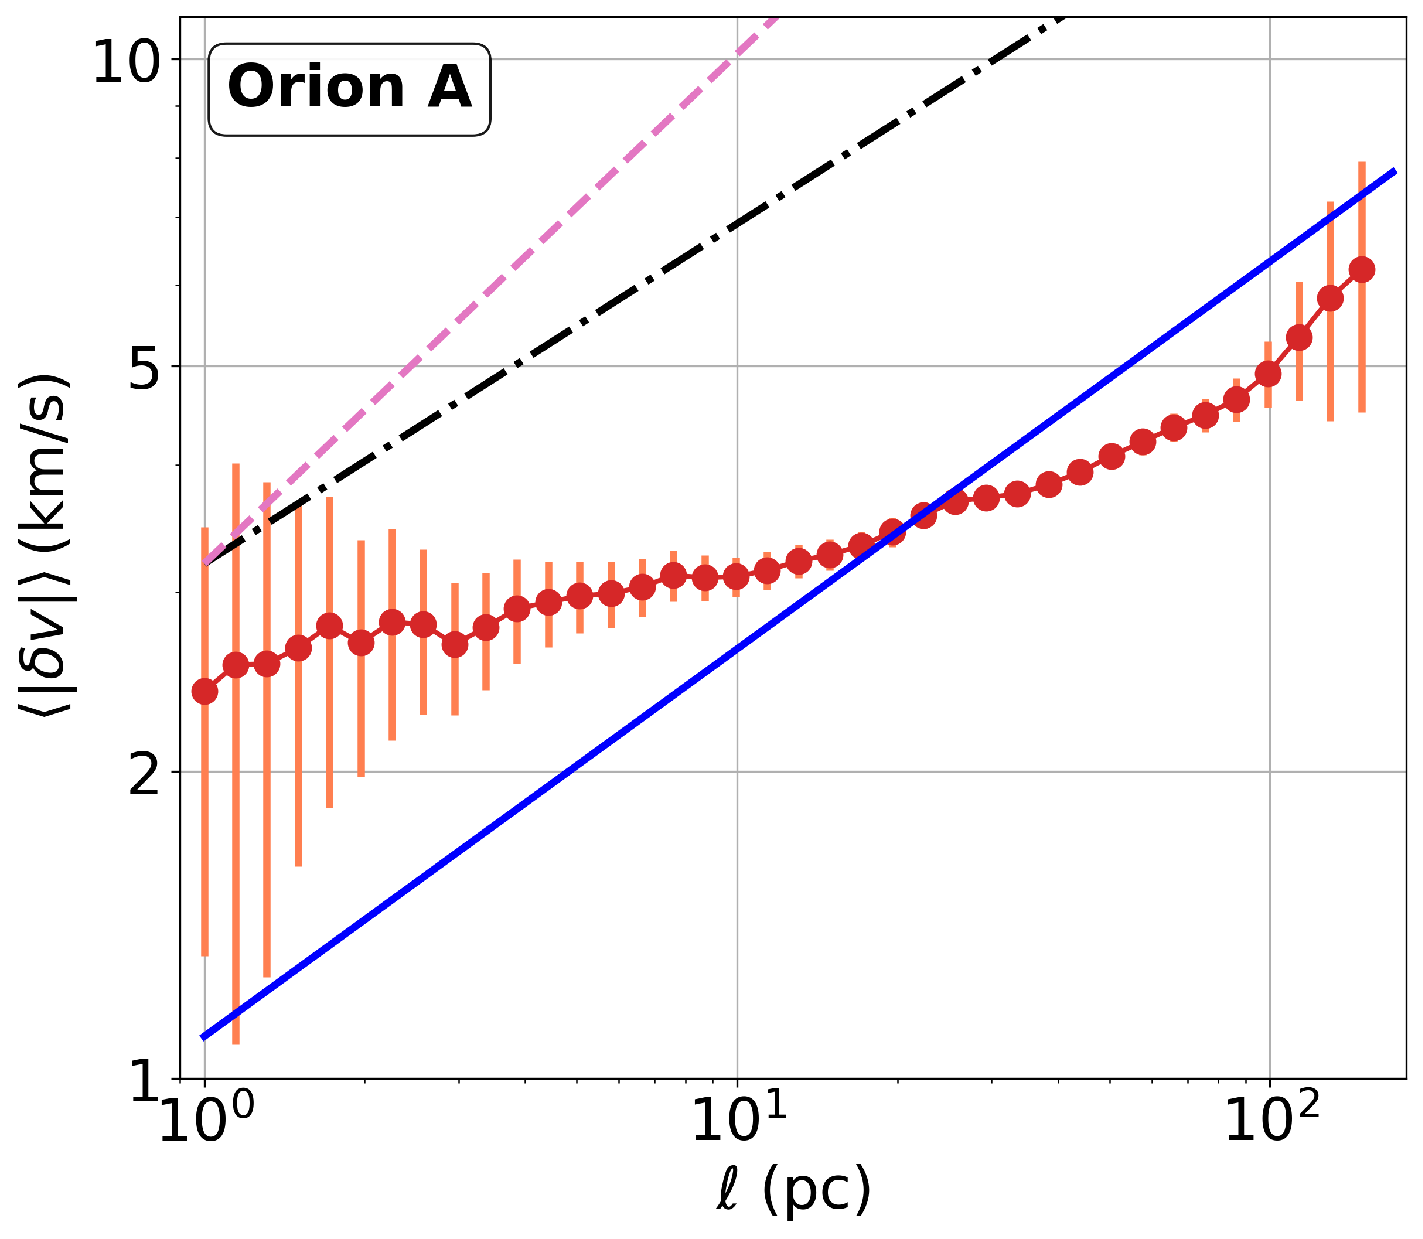
\includegraphics[width=0.32\linewidth]{Stars_img/VSF_OrionA.pdf}
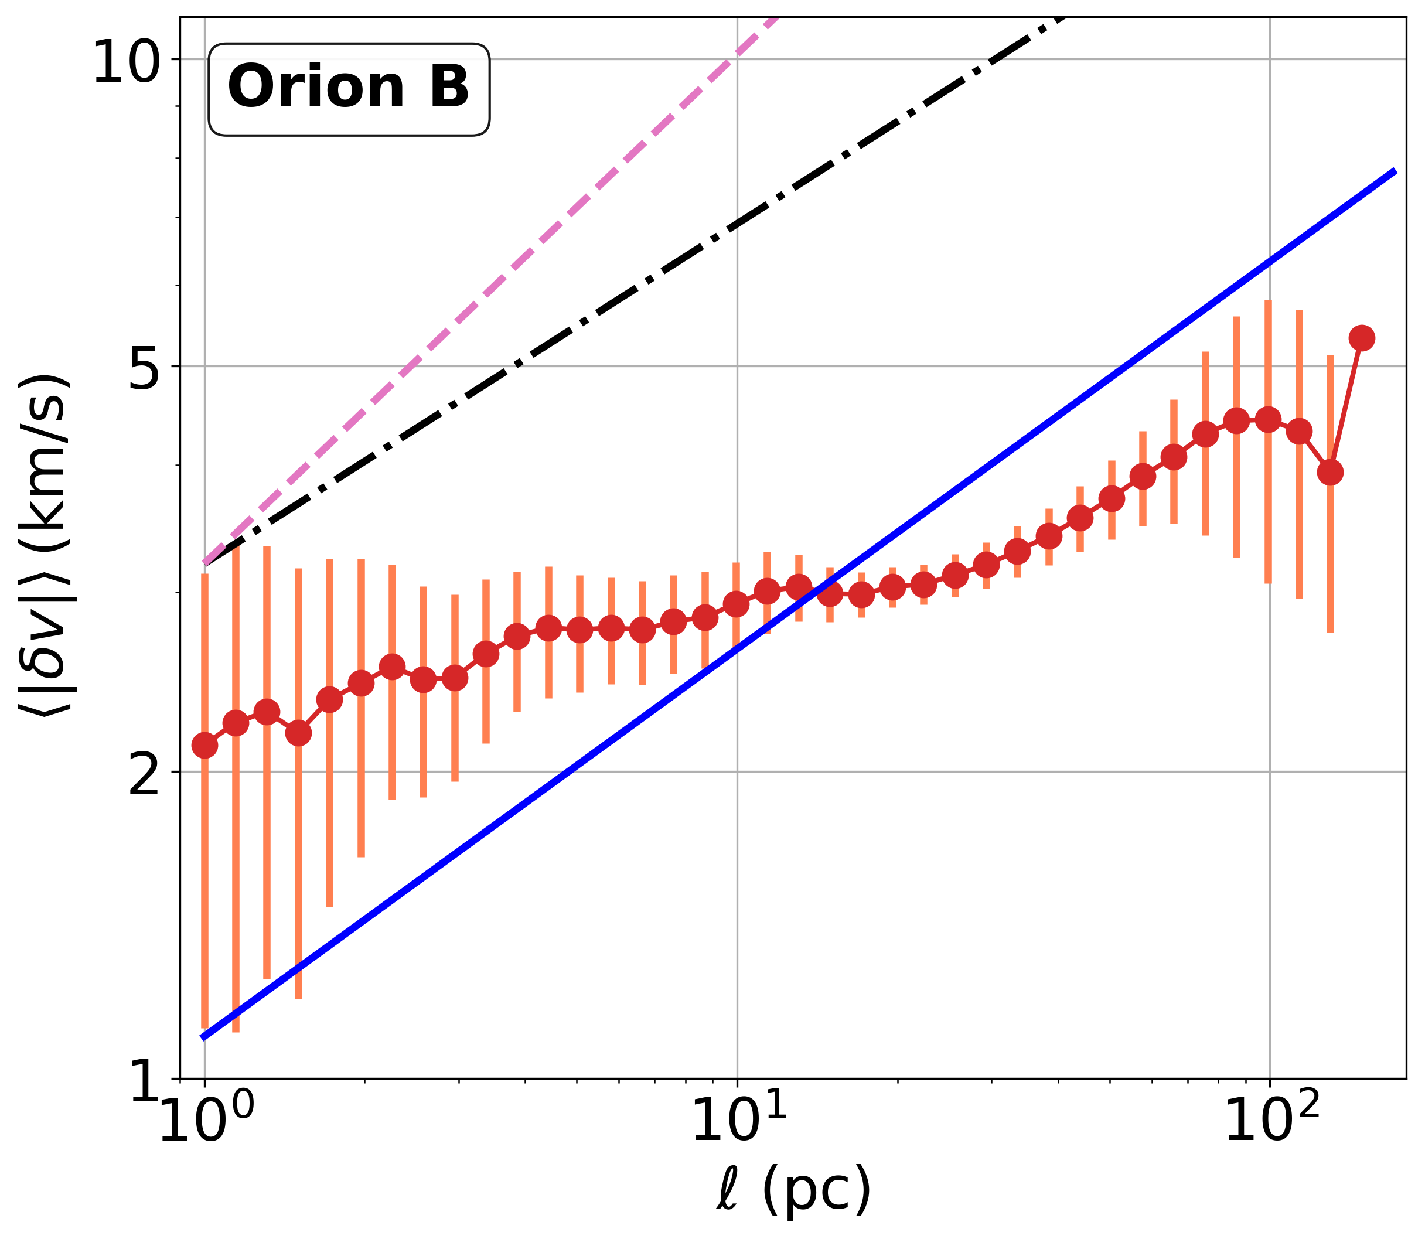
\includegraphics[width=0.32\linewidth]{Stars_img/VSF_OrionB.pdf}
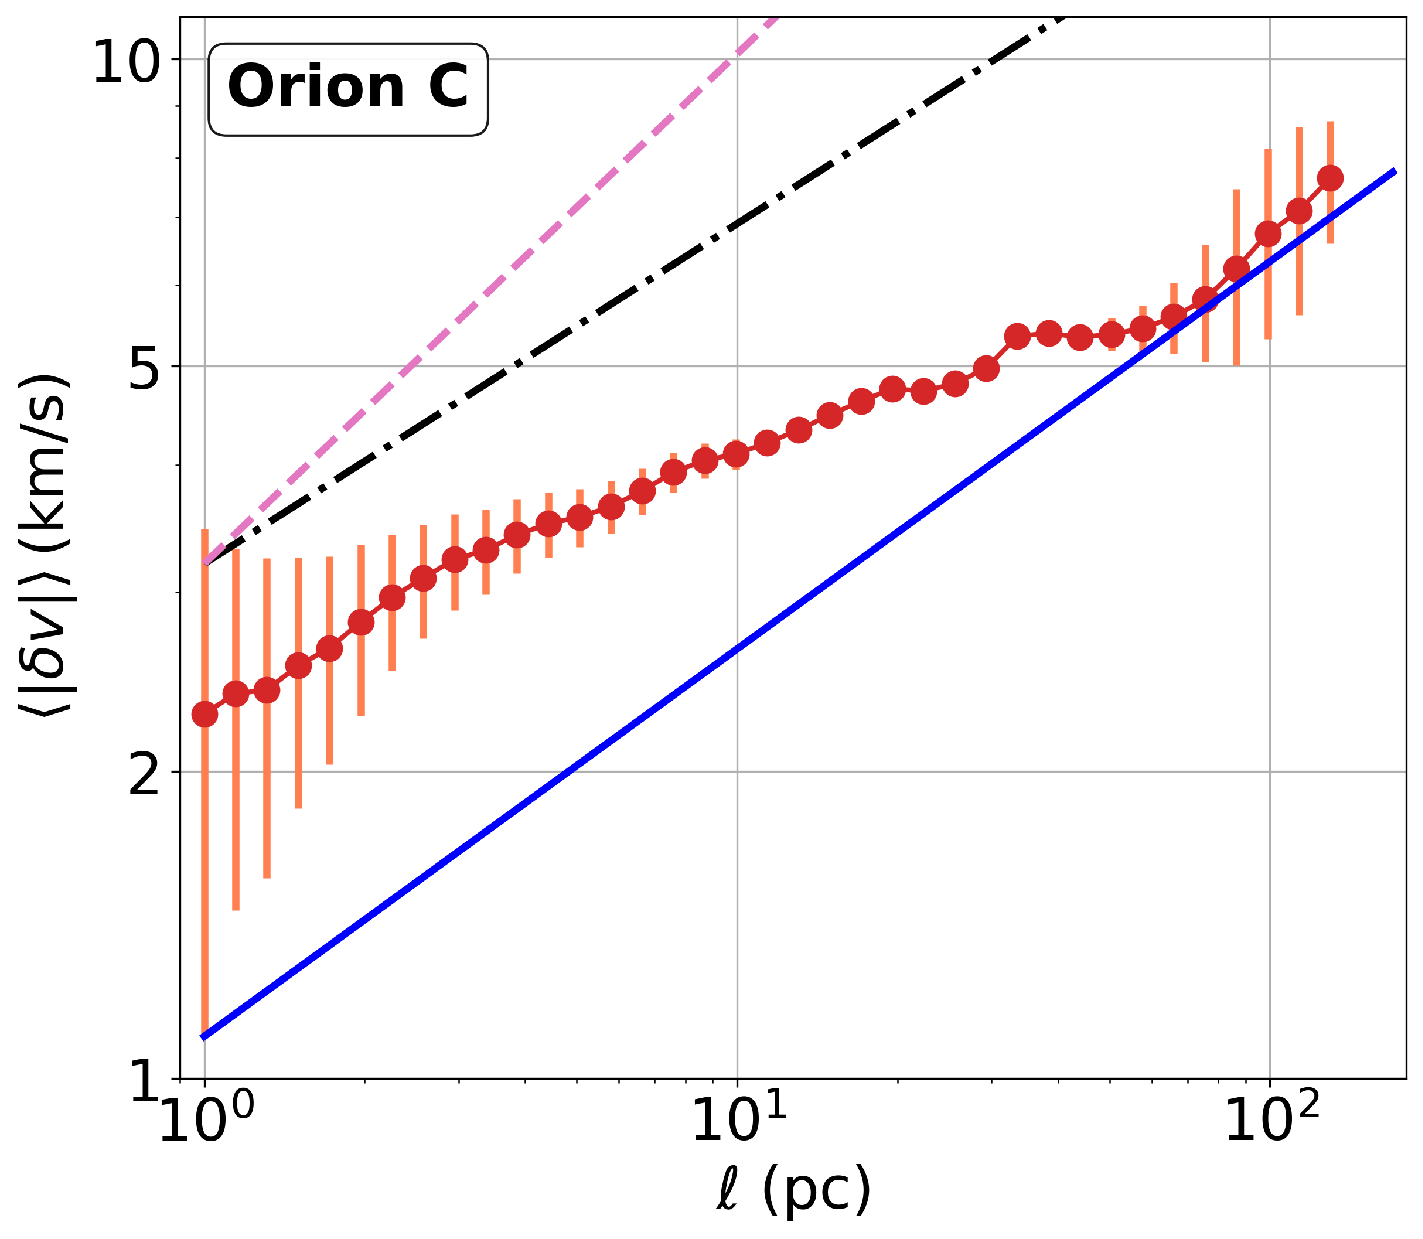
\includegraphics[width=0.32\linewidth]{Stars_img/VSF_OrionC.pdf}\\
\vskip 0.1in
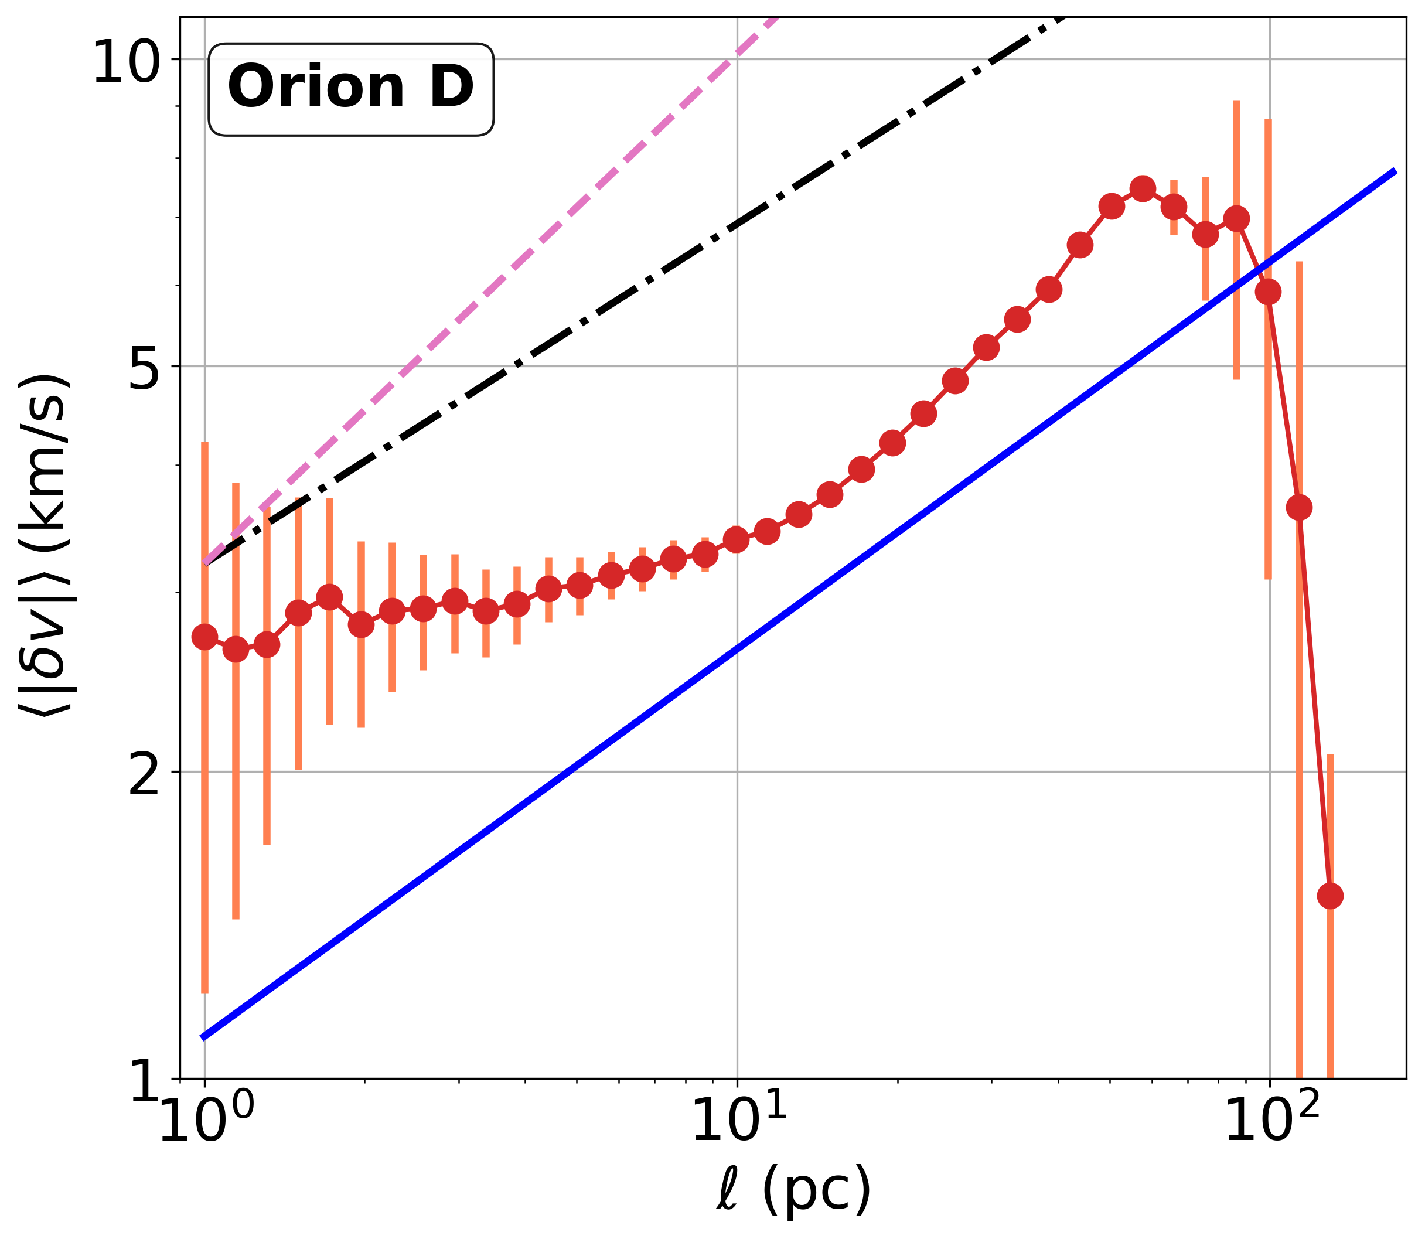
\includegraphics[width=0.32\linewidth]{Stars_img/VSF_OrionD.pdf}
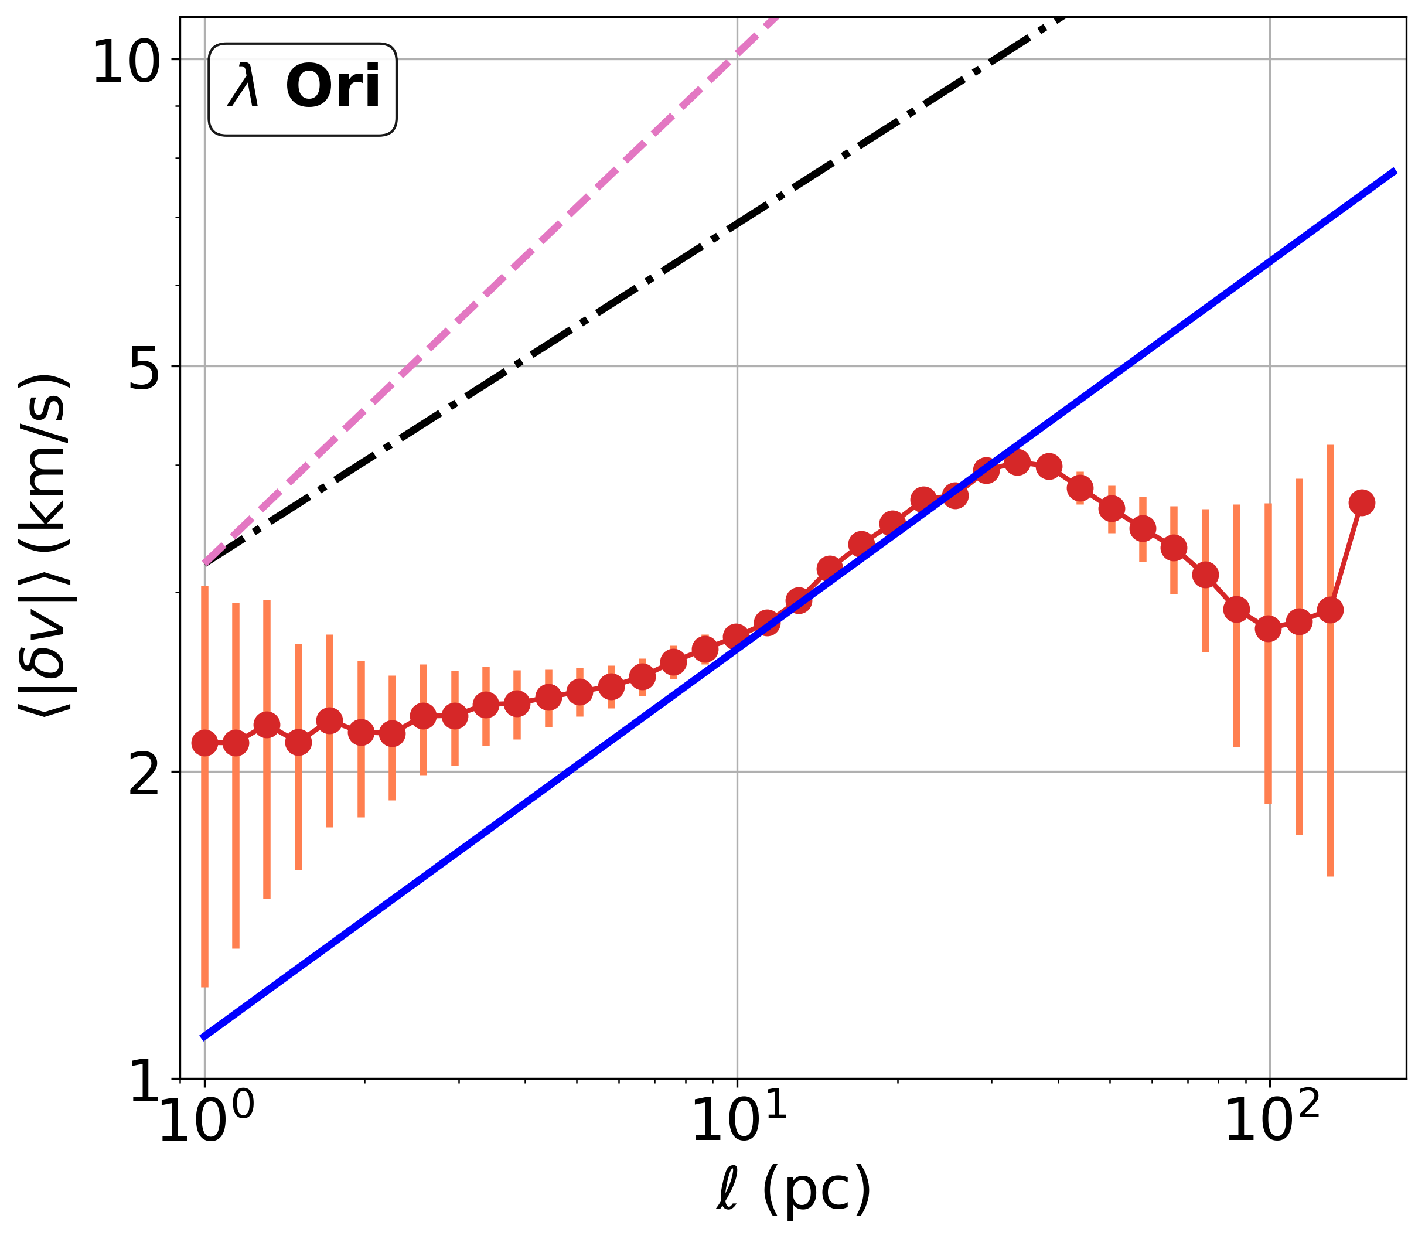
\includegraphics[width=0.32\linewidth]{Stars_img/VSF_LambdaOri.pdf}
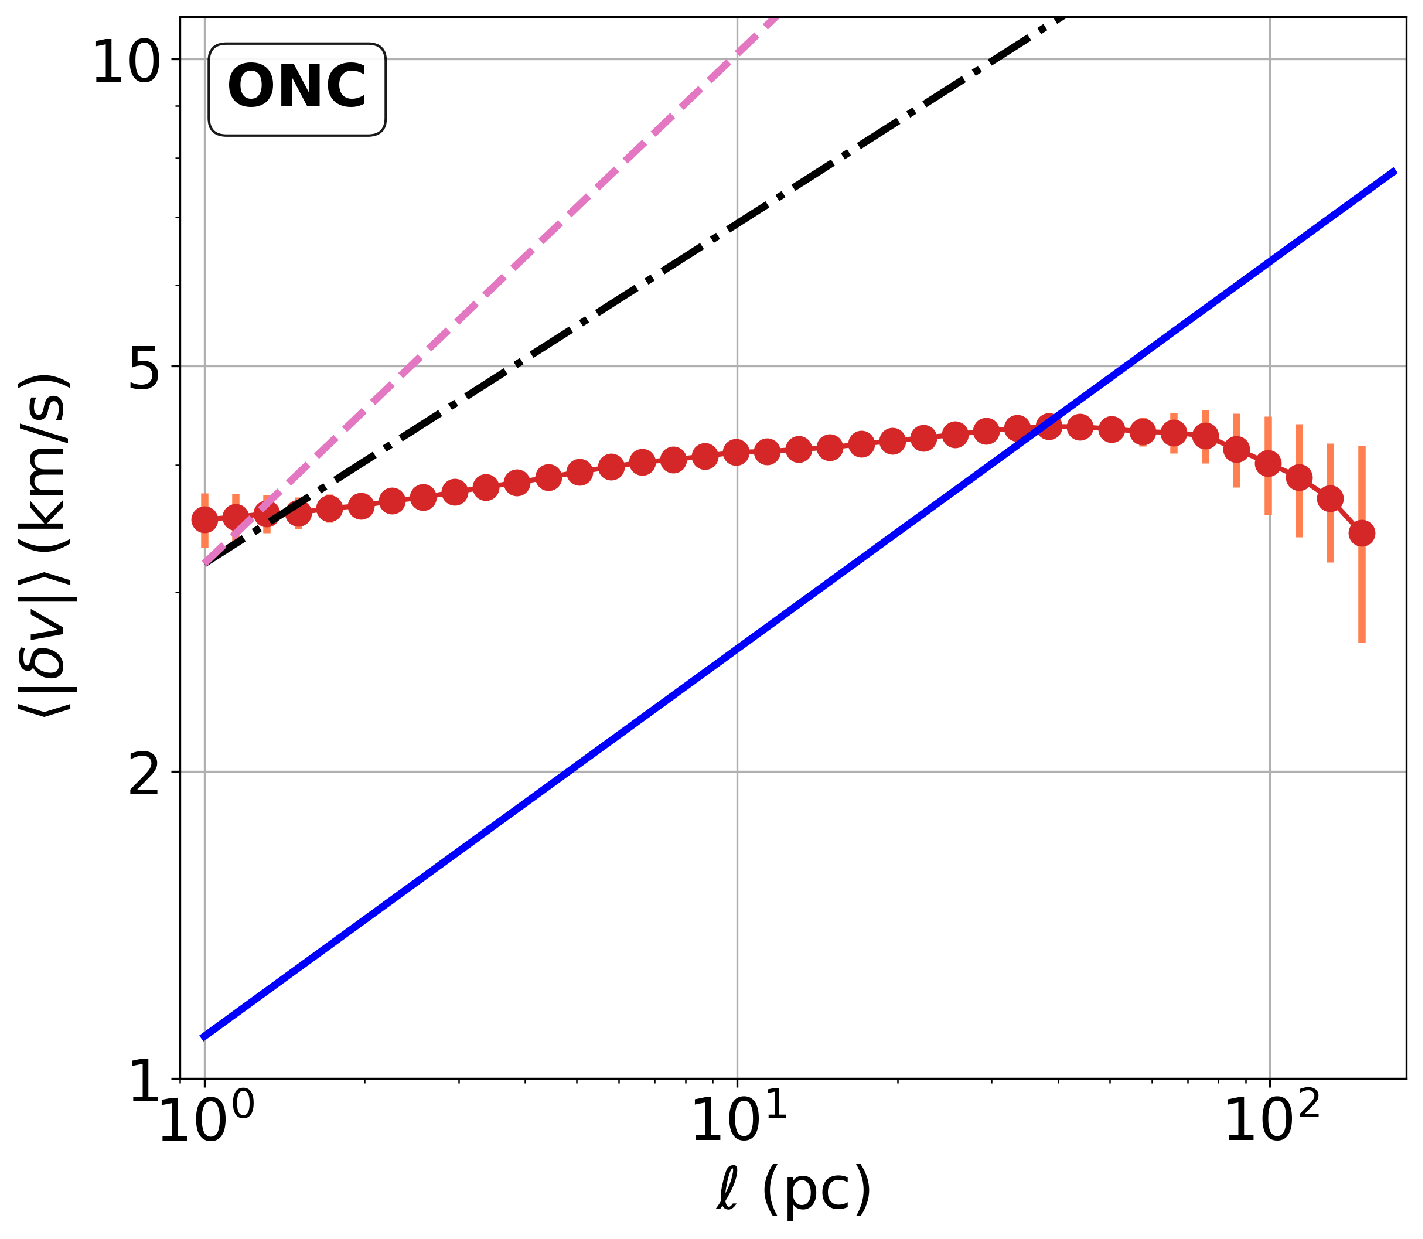
\includegraphics[width=0.32\linewidth]{Stars_img/VSF_ONC.pdf}\\
\vskip 0.1in
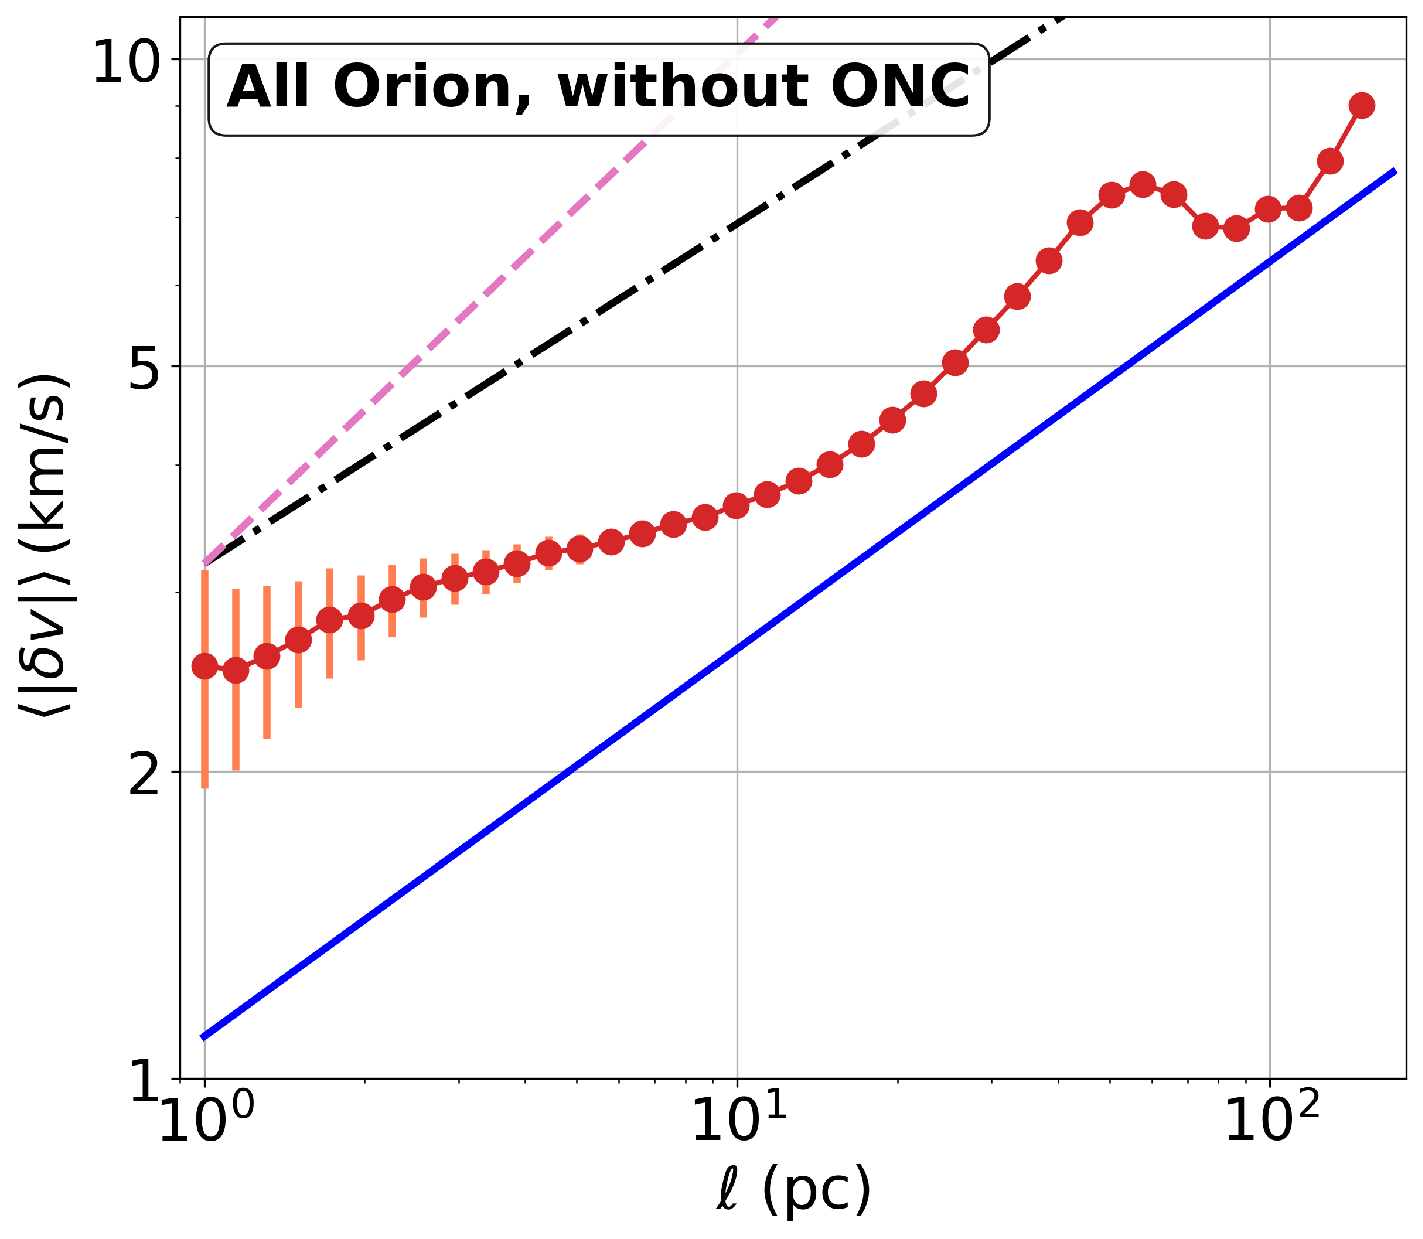
\includegraphics[width=0.32\linewidth]{Stars_img/VSF_Orion_noONC.pdf}
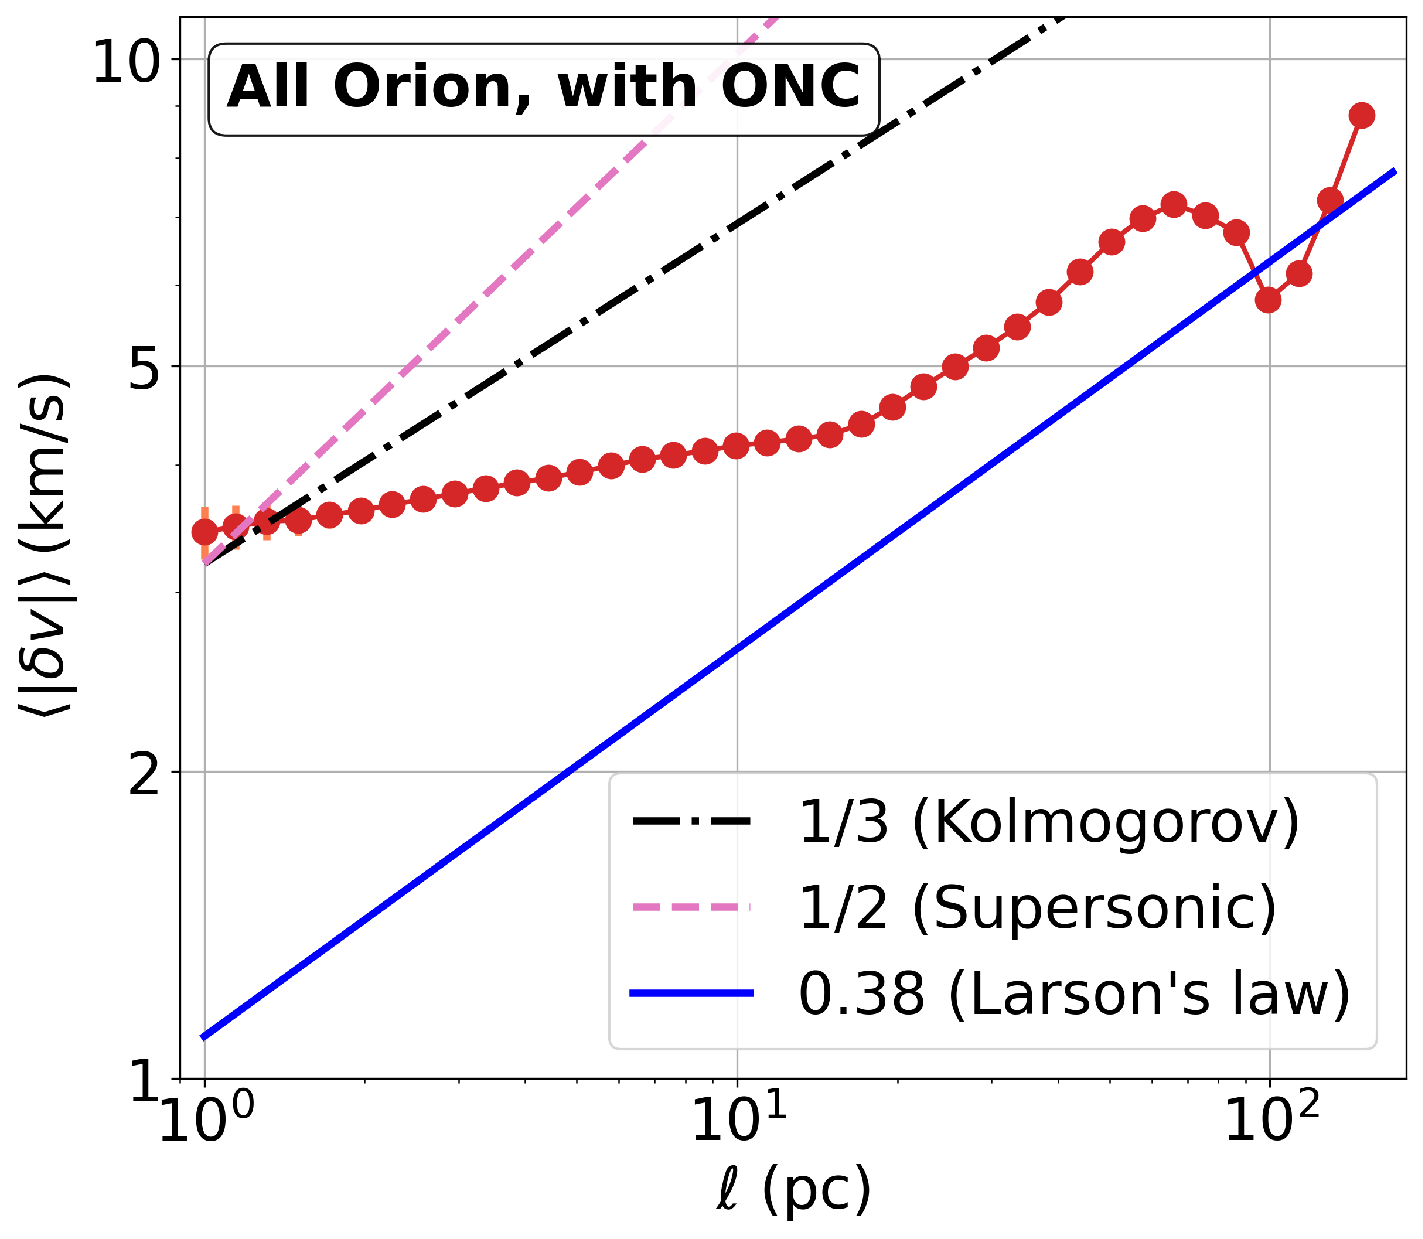
\includegraphics[width=0.32\linewidth]{Stars_img/VSF_Orion_withONC.pdf}
\caption{Left to right, top to bottom: first-order VSF of stars in the Orion A, Orion B, Orion C, Orion D, Lambda Ori, ONC, all Orion without ONC, and all Orion with ONC\@. The error bars are obtained through a random sampling analysis, and represent the uncertainties from both observational errors and uncertainties due to small sample size. As reference, we also plot a black dot-dashed line of slope 1/3 for the Kolmogorov turbulence, a pink dashed line of slope 1/2 for supersonic turbulence, and a solid blue line for Larson's velocity dispersion correlation for molecular clouds: $\sigma (km \cdot s^{-1}) = 1.1 \cdot L (pc)^{0.38} $ \citep{larson_turbulence_1981}. All panels use 40 logarithmic bins of $\ell$ from 1 pc to 170 pc. }\label{fig:vsf}
\end{figure*}

\subsection{Results}\label{sec:orion-results}

\subsubsection{The first-order VSFs}

Figure~\ref{fig:vsf} shows the first-order VSF of stars in all six individual groups in the Orion Complex. The last two panels show the combined VSF of all groups without and with the ONC, respectively. 
To guide the eye, we also plot in each panel the expected scaling for supersonic and subsonic turbulence, along with Larson's law measured for turbulence in molecular clouds in the Milky Way \citep{larson_turbulence_1981}.

The VSFs of all six individual groups except ONC exhibit a power-law scaling, characteristic of a turbulent flow. The amplitudes and slopes vary from group to group. The best-fit VSF slopes are listed in Table~\ref{table:data}.

The Orion A group (top left panel of Figure~\ref{fig:vsf}) is located just outside of Barnard's Loop (the shell-like feature to the left of Orion A-D in Figure~\ref{fig:orion}, see also \citet{ochsendorf_nested_2015}), which is proposed to have originated from a supernova that erupted $\sim$6 Myr ago \citep{kounkel_supernovae_2020}. Due to its location, Orion A is largely unaffected by the supernova's shock wave. Indeed we observe that its VSF slope generally follows that of subsonic turbulence. The overall amplitude is slightly below Larson's relation. 

The Orion B cloud is connected to Orion A but closer to the center of the supernova explosion. Our analysis of the Orion B group suffers from high uncertainties due to low number of stars (51) available in the catalog. The slope of the VSF of Orion B (top middle panel) is not well constrained, but the VSF generally follows the turbulence-like kinematics present in other clouds. The amplitude is roughly consistent with Larson's relation.

Orion C lies within the supernova bubble, and as \citet{kounkel_supernovae_2020} suggested, was driven apart from Orion D at the opposite front of the supernova shock wave. Most of the stars in Orion C and D formed after the supernova explosion that created the Barnard's Loop. We observe this local energy injection effect on the VSF of Orion C (top right panel) with a higher-than-Larson amplitude. 
The slope of the VSF is flatter than the Kolmogorov turbulence due to the presence of $\sigma$ Ori, a dense cluster of age $\sim$2 Myr. We discuss the effects of dense clusters on the VSF in more detail later in this section. 

Stars in the Orion D group exhibit a curious VSF (middle left panel), with a slope more in line with supersonic turbulence (slope $1/2$) than Kolmogorov at distance scale $10<\ell<60$ pc and absolute velocity difference higher than that of Larson's law. We attribute these properties of Orion D's VSF to its position inside the supernova bubble. Located close by and at the front of the bubble (in our line-of-sight) as it expands, motion of stars in the Orion D cloud is additionally driven by the shock wave of the supernova, hence its turbulent kinetic energy is amplified. 


The last independent group we look at is $\lambda$ Ori (center panel of Figure~\ref{fig:vsf}). In the $10<\ell<32$ pc range, the VSF of stars in $\lambda$ Ori closely exhibits the 0.38 slope of Larson's law. The amplitude also exactly follows Larson's relation \citep{larson_turbulence_1981}, and is higher than Orion A and B, but lower than Orion C and Orion D. This result can be understood given $\lambda$ Ori's history and isolated position in the Orion Complex. The $\lambda$ Orion bubble (the bubble-like structure surrounding $\lambda$ Ori in Figure~\ref{fig:orion}) is proposed to have been created by a supernova explosion $\sim1$ Myr ago \citep{dolan_photometric_2002}. Although \citet{kounkel_supernovae_2020} estimated the age of the remnant to be $\sim 4$ Myr. Regardless, the explosion happened after many of the stars have already formed in $\lambda$ Ori where the stellar age has a wide spread over $\sim 6$ Myr \citep{kounkel_apogee-2_2018}. Thus the effect of local energy injection is not as prominent as in Orion C and D.

The ONC's VSF (middle right panel) has a distinctively flatter slope compared to other groups in the Orion Complex. The ONC is a dense star cluster located at one end of the Orion A molecular cloud (Figure~\ref{fig:orion}). Unlike the loose star groups discussed previously, the ONC has a dense inner core ($\sim 2$ pc) with an estimated relaxation time of $\tau_r \sim$ 0.6 Myr \citep{hillenbrand_preliminary_1998}, shorter than the cluster's mean age of $\sim$ 2.6 Myr. Therefore, a significant fraction of the stars in the ONC have dynamically relaxed, and have hence ``forgotten" the turbulence kinematics of their natal clouds. The residual non-zero slope likely originates from the stars in the outer parts of the cluster that have not relaxed yet. It is worth noting that if we simply look at the velocity distributions of stars in different groups (Figure~\ref{fig:velodist}), ONC does not appear drastically different from the rest of the groups apart from its compactness in the velocity space. Yet our analysis reveals its distinct kinematics due to relaxation.

In the last two panels of Figure~\ref{fig:vsf}, we compute the VSF for all the stars within the Orion Complex without and with the ONC (bottom left and bottom right panels, respectively). Without the ONC, the VSF of the Orion Complex has similar characteristics to that of Orion D, with a steeper-than-Kolmogorov slope and an amplitude higher than Larson's law in the $10<\ell<60$ pc scale range. This is because D has the highest number of stars amongst the 5 groups (Table ~\ref{table:data}). 

When the ONC is included, on small scales ($2<\ell<20$ pc), the VSF flattens because it is heavily influenced by the cluster due to its dominant number of stars in the catalog (585 stars vs. a total of 1439 stars). In fact, this is why we separate the ONC from Orion A in our analysis. If we include ONC in Orion A, the resulting VSF is significantly flatter. All the other star groups also contain star clusters. For example, Orion C has $\sigma$ Ori. We do not separate these clusters because they are much smaller than the ONC, and removing them degrades the statistics of our analysis. We note, however, that they may have contributed to the flatter VSF of Orion C and the flattening of the VSF in the other groups on small scales. We discuss other uncertainties in more detail in Section~\ref{sec:discussions}. 

The combined VSF shows a bump at $\sim 60$ pc, similar to Orion D, suggesting energy injection at that scale. The mean age of the stars in this study is $\sim 3.7$ Myr. Given the current size of the Barnard's loop ($\sim 80$ pc) and its age ($\sim 6$ Myr), the energy injection scale is roughly consistent with the size of the supernova bubble when the stars first formed. This again shows the effects of local energy injection of supernova explosions on turbulence.



\subsection{Discussions}\label{sec:discussions}

\subsubsection{Biases and Uncertainties}

Gas in molecular clouds such as the Orion Complex is turbulent by nature. The theoretical foundation of our analysis is that newborn stars retain this turbulence information. However, after the stars are born, they decouple from the hydro-dynamical forces of the gas, and no longer follow the turbulent flow. In other words, stars are only perfect tracers of turbulence at birth. Since star formation happens over a period of time, all of the star groups contain stars that are over a few Myr old. We have identified two mechanisms through which stars can lose their memory of the ISM turbulence, causing biases in our analysis.

The first mechanism is dynamical relaxation, which we discussed in the analysis of the ONC in Section~\ref{sec:orion-results}. Due to open clusters' high density, close stellar encounters are common, which alter the stars' original orbits and lead to dynamical relaxation. The relaxation time is estimated as a function of the number of stars and the crossing time of the cluster:

\begin{equation}
t_{relax} = t_{cross} \cdot \frac{N}{6 \cdot \ln{N/2}} \,,
\end{equation}
where $N$ is the total number of stars in the cluster and $t_{cross}$ is the crossing time, defined as the typical time for a star to travel a distance equal to the half-mass size of the cluster:

\begin{equation}
t_{cross} =  \frac{2 \cdot R_{hm}}{\sigma_v} \,.
\end{equation}
Here, $R_{hm}$ is the radius within which half of the cluster's stars reside, and $\sigma_v$ is the bulk-motion-removed characteristic velocity of the cluster's stars. It is computed as the standard deviation of the velocity distribution with respect to the median \(\sigma_v \equiv \sigma [|v_i - v_{median}|]\).

After the stars are relaxed, they no longer hold the turbulent kinematics of gas at the time of their formation. For loose groups of stars such as those we analyze, the crossing times are significantly longer than the group's current age (Table~\ref{table:data}). Furthermore, since each group possesses a number of stars in the order of N $\sim 10^3$ (e.g., N = 2800 stars within the dense core of the ONC was used by \citet{hillenbrand_preliminary_1998}), the estimated relaxation time is an order of magnitude longer than the crossing time. Therefore, dynamical relaxation has most likely not affected the shape of the VSF for the five groups in the Orion Complex, except for the ONC\@. This is in agreement with \citet{da_rio_-sync_2017} who find that young stars in Orion A are kinematically associated with the molecular gas, but the ONC appears more dynamically evolved and virialized. \citet{kounkel_apogee-2_2018} also found consistent kinematics between young stars and gas in the whole Orion Complex where the gas has not been dispersed.

In addition to the ONC, there are other clusters within each group: $\sigma$ Ori in Orion C, 25 Ori in Orion D, $\lambda$ Orionis Cluster in $\lambda$ Ori, and two small clusters NGC 2024 and NGC 2068 in the Orion B group. These clusters have much smaller physical sizes than the ONC and contain only a small fraction of stars of the group. This property of the clusters can be visually confirmed from Figure~\ref{fig:orion}. Thus, their existence does not significantly affect our overall results. However, they may have contributed to the flattening of the VSFs on small scales that we observe in almost all individual groups.

Another potential source of bias in our analysis comes simply from the drifting of stars from their original positions. Assuming no strong stellar encounters, stars with higher velocity differences drift apart at a faster rate than stars with smaller velocity differences, causing the VSF to steepen with time. This steepening happens over roughly $t_{cross}$.

In our analysis, most groups are relatively young, with their ages much shorter than $t_{cross}$ (Table~\ref{table:data}), so drifting should not have had time to erase turbulence-driven velocity differences. Although drifting may have steepened the VSF of Orion D, which has the oldest median age and the steepest slope amongst all the groups analyzed here. We plan to further explore the effects of relaxation and drifting in our future works both with a larger observed sample and with numerical simulations \citep{li_disruption_2019}. 

There are also other sources of uncertainties in our analysis, such as binary systems. While the barycenter should follow the turbulent velocity of the natal cloud, binaries also have orbital motion contributing to the overall velocity measurement. While most systems with very large orbital speeds have been excluded from the analysis through the initial hierarchical clustering, systems with orbital speeds of only a few km s$^{-1}$ likely remain.

False positives in hierarchical clustering, such as contamination from the field stars, can also affect our results. \citet{kounkel_apogee-2_2018} estimated that false positive fraction for the clustering algorithm can be as high as $\sim$6\%. In addition, drifting can result in close pairs of uncorrelated stars with high relative velocity. Binaries, drifting, and mis-grouped stars, coupled with small sample sizes at small separations would explain the flattening of the VSFs at small $\ell$.

\subsubsection{Comparison with other Methods to Measure Turbulence}
Most of the previous studies on turbulence in astrophysical environments rely on the observations of gas. Although only velocity statistics can directly 
reflect the dynamics of turbulence and turbulent energy cascade, 
it is the density statistics that is widely used for measuring turbulence as it is much more easily accessible to observations. For example, the delta-variance method has been used to analyze the structure of observed molecular cloud images in the ISM \citep{stutzki_fractal_1998}. The same method and a modification of it \citep{arevalo_mexican_2012} have also been used to infer turbulence in the hot intracluster medium based on X-ray images \citep[e.g.,][]{zhuravleva_turbulent_2014}.%

Velocity centroids can recover the turbulent velocity spectra in subsonic turbulence 
\citep{esquivel_velocity_2005}. 
The velocity channel analysis (VCA)
using channel maps and 
velocity coordinate spectrum (VCS)
using the fluctuations 
measured along the velocity axis of the Position--Position--Velocity (PPV) cubes
can also be used to extract turbulent velocity spectra in supersonic turbulence
(see \cite{lazarian_obtaining_2009} for a review). 
In particular, the VCS technique only requires measurements along a few directions to obtain a reliable velocity spectrum
\citep{chepurnov_turbulence_2009}. Spectroscopic data has also been used in the Principal Component Analysis to extract the size-line width relation and recover the structure function within molecular clouds, as reported by \citet{heyer_universality_2004} and \citet{roman-duval_turbulence_2011}.

Recently, statistical measurements of the velocities of gas phase point sources have been developed for, e.g., dense molecular cores embedded in the background turbulent flow \citep{qian_13co_2012} and filaments in the centers of galaxy clusters \citep{li_direct_2020}. These analyses use the 1D line-of-sight velocities and 2D positions projected on the plane of the sky. The bias due to the projection effect depends on the thickness of the structure \citep{qian_new_2015}, which is usually unknown.

Our analysis in spirit is similar to that of gas phase point sources, but instead of using projected information, we take advantage of the full 6D (3D velocity + 3D position) information of stars. Thus our results do not suffer from the poorly constrained projection uncertainties. Observing 6D information of the gas, especially the motions in the plane of the sky, is prohibitively challenging \citep[although see][]{odell_high_2008}. Thus our method has a unique advantage, and can potentially be used to help better understand the biases in the analyses based on gas.


\subsubsection{Comparison with Theories and Other Observations}

There has been a lot of previous work on turbulence in Orion based on the observations of emission lines of the ionized gas \citep{castaneda_velocity_1988, odell_motion_1992, mcleod_nebular_2016, arthur_turbulence_2016}. Most of them are focused on small scales ($<1$ pc) and therefore cannot be directly compared with our results. But they do generally find VSFs consistent with turbulence, in agreement with our results.

On larger scales (a few to $\sim 100$ pc), we have compared our results with Larson's Law in Section~\ref{sec:orion-results}. Individual groups may show slightly higher or lower amplitude than the mean Larson's relation, with slightly steeper or shallower slopes, but overall, our results are in good agreement with Larson's Law for molecular clouds in the Milky Way. Notably, \citet{larson_turbulence_1981} also finds a slightly lower-than-average amplitude for Orion B, consistent with our findings here even though we are using different tracers of turbulence. 

Our results show that regions heavily influenced by supernova explosions can exhibit a higher level of turbulence, and even a steeper VSF\@. This is consistent with numerical simulations showing that supernovae can drive turbulence in molecular clouds \citep{padoan_supernova_2016}.
Additionally, the steepened slope of Orion D is consistent with \citet{federrath_universality_2013} finding that supernova explosions excite more compressible than solenoidal velocity modes in the gas, which tends to steepen the VSFs, and thus exhibit the 1/2 power law of supersonic turbulence. Observations have also shown the local effects of supernovae on turbulence in other systems (e.g., in the Large Magellanic Clouds \citep{szotkowski_mapping_2019}). 

\subsection{Concluding Remarks and Future Work}
We have introduced a new method to study turbulence in the ISM using motions of 
young stars. Our results demonstrate that stars in young star groups retain the memory of turbulence of their natal molecular clouds. Our analysis uses the full 6D information of stars to trace turbulence, and does not suffer from projection uncertainties. Our results can be used to provide independent constraints on the turbulent properties of molecular clouds in addition to analysis of gas kinematics, and also shed light on studies of the dynamical evolution of star clusters in the Galaxy \citep{kamdar_dynamical_2019}. 

We plan to apply our analysis to a much larger sample of star groups in the future. Meanwhile, we will perform and analyze tailored numerical simulations of star formation in molecular clouds to better understand biases and uncertainties in our analysis, as well as constraining subgrid models for star formation \citep{li_disruption_2019}. 

\subsection{Supplemental Material}

\subsubsection{The higher-order VSFs}
\label{subsec:high_order}

We present the second and third order VSFs in Figure~\ref{fig:3rdorder}.
High order VSFs are usually used to evaluate the intermittency
\citep{she_universal_1994,boldyrev_supersonic_2002}.
Different behaviors of the high-order VSFs measured with different gas tracers, e.g., $H_2$, $CO$, were found in numerical simulations of molecular clouds,
which are related to their different volume filling factors and spatial distribution
\citep{bertram_centroid_2015}.
The second and third order VSFs that we present in Figure~\ref{fig:3rdorder}
are generally consistent with the Kolmogorov scaling. This finding agrees with the
measurement using the velocities of dense cores in Taurus cloud
\citep{qian_studies_2018}.
It suggests that both the dense cores and the stars used here sample the turbulence in the relatively diffuse region with a large volume filling factor, and thus the Kolmogorov scaling is expected \citep{xu_projected_2020}.

\label{sec:2ndvsf}
\begin{figure}
    \centering
    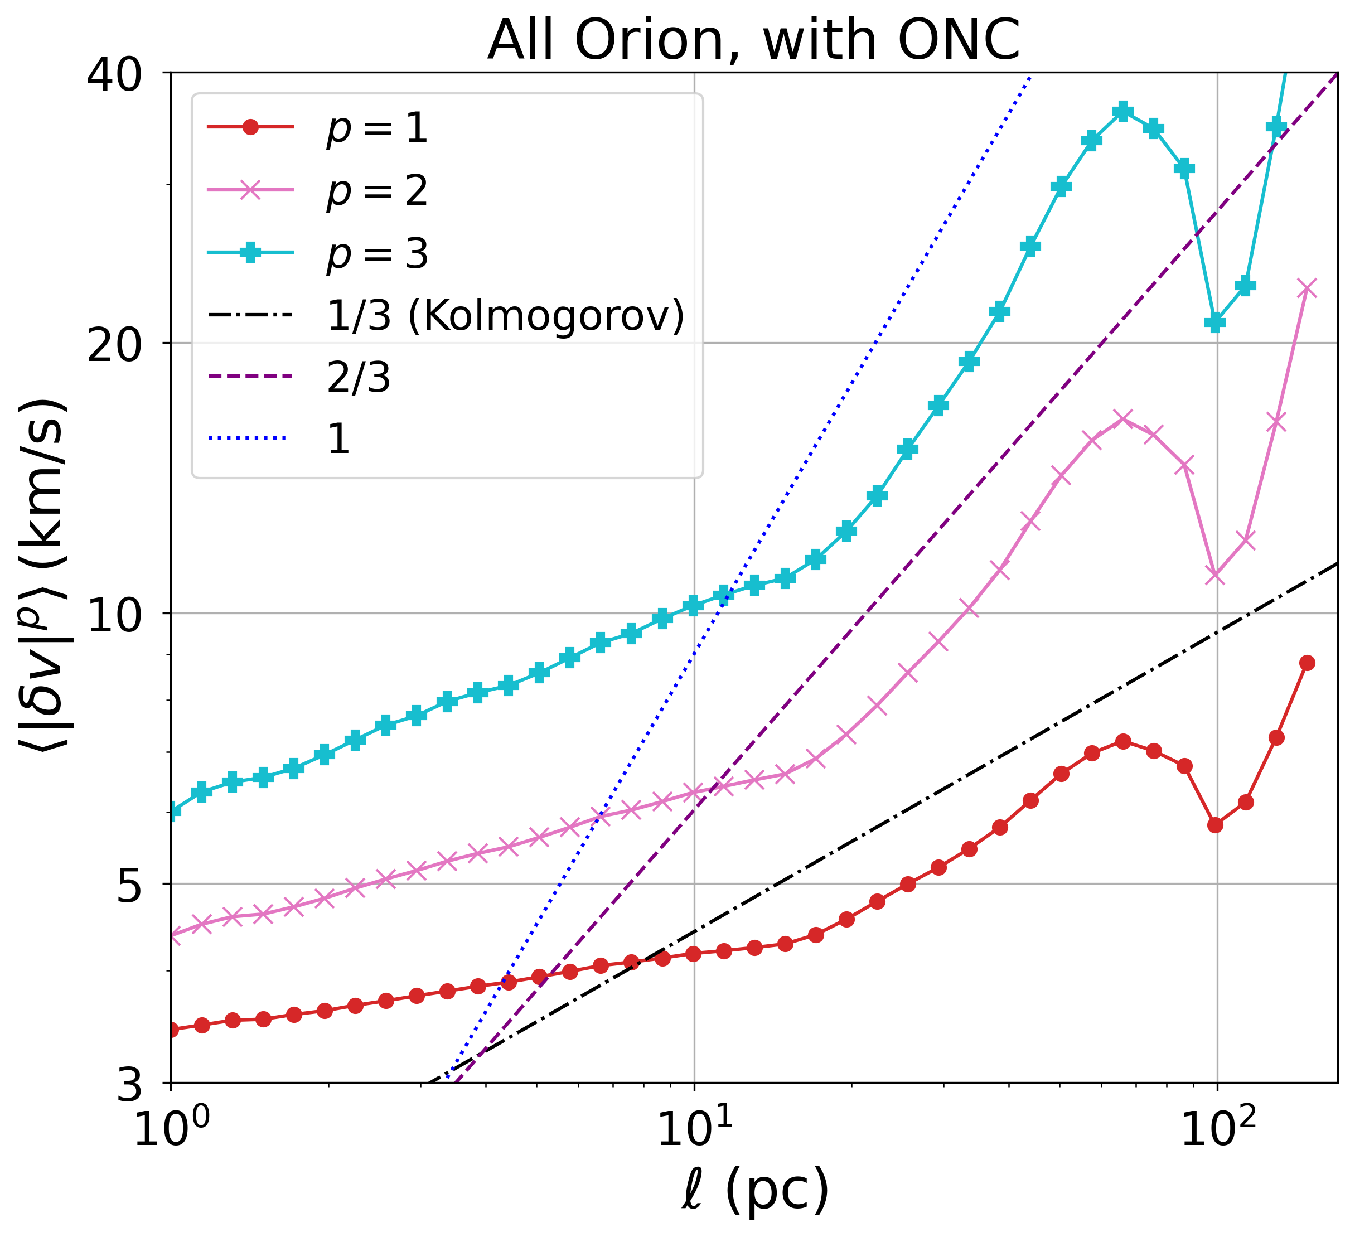
\includegraphics[width=0.7\linewidth]{Stars_img/3rdorder_Orion.pdf}
    \caption{First ($p=1$, red), second ($p=2$, pink), and third ($p=3$, blue) order VSFs of the stars in the entire Orion Complex. The second and third order VSFs have been shifted lower for easy comparison.}
    \label{fig:3rdorder}
\end{figure}


\section{Ophiuchus, Perseus, Taurus, and Comparing Stellar Motion Against Gas}

\publicationdetails
{Ha et al. 2022, ApJ, 934, 7}
{Trung Ha\footnotemark[1], Yuan Li\footnotemark[1], Marina Kounkel\footnotemark[2], Siyao Xu\footnotemark[3]\footnotemark[4], Hui Li\footnotemark[5]\footnotemark[4], and Yong Zheng\footnotemark[6]}
{The interstellar medium (ISM) is turbulent over vast scales and in various phases. In this paper, we study turbulence with different tracers in four nearby star-forming regions: Orion, Ophiuchus, Perseus, and Taurus. We combine the APOGEE-2 and Gaia surveys to obtain the full six-dimensional measurements of positions and velocities of young stars in these regions. The velocity structure functions (VSFs) of the stars show a universal scaling of turbulence. We also obtain \halpha~gas kinematics in these four regions from the Wisconsin H-Alpha Mapper. The VSFs of the \halpha~are more diverse compared to those of stars. In regions with recent supernova activities, they show characteristics of local energy injections and higher amplitudes compared to the VSFs of stars and of CO from the literature. Such difference in amplitude of the VSFs can be explained by the different energy and momentum transport from supernovae into different phases of the ISM, thus resulting in higher levels of turbulence in the warm ionized phase traced by \halpha. In regions without recent supernova activities, the VSFs of young stars, \halpha, and CO are generally consistent, indicating well-coupled turbulence between different phases. Within individual regions, the brighter parts of the \halpha~gas tend to have a higher level of turbulence than the low-emission parts. Our findings support a complex picture of the Milky Way ISM, where turbulence can be driven at different scales and inject energy unevenly into different phases.}
{\footnotetext[1]{Department of Physics, University of North Texas, Denton, TX 76203, USA}
\footnotetext[2]{Physics \& Astronomy Department, Vanderbilt University, PMB 401807, 2301 Vanderbilt Place, Nashville, TN 37235, USA}
\footnotetext[3]{Institute for Advanced Study, 1 Einstein Drive, Princeton, NJ 08540, USA}
\footnotetext[4]{NASA Hubble Fellow}
\footnotetext[5]{Department of Astronomy, Columbia University, 550 West 120th Street, New York, NY 10027, USA}
\footnotetext[6]{Department of Astronomy, University of California, Berkeley, CA 94720, USA}}
\setcounter{footnote}{0}

\subsection{Introduction} \label{sec:multi-region-intro}

The interstellar medium (ISM) is multiphase and turbulent. Interstellar turbulence affects the velocity statistics on all scales from the diffuse ionized gas to the dense molecular gas. \citet{larson_turbulence_1981} compiled the internal velocity dispersion of nearby molecular clouds from the width of various emission lines, and found a power-law relation between the velocity dispersion and cloud size, with slope 0.38, between the 1/3 slope expected for turbulence dominated by solenoidal motions \citep{kolmogorov_local_1941} and the 1/2 slope expected for shock-dominated turbulence \citep[e.g.,][]{galtier_exact_2011,federrath_universality_2013}.

Inside molecular clouds, massive O- and B-type stars create \ion{H}{2} regions by ionizing and heating the ISM with UV radiation \citep[see, e.g.,][]{spitzer_physical_1978}. 
Compression from supernova (SN) explosions can trigger further star formation \citep[][]{kennicutt_star_2012}. Interstellar processes such as SNe, stellar winds, ionizing radiation, and cosmic rays all play a role in maintaining the structure of the ISM, as well as in regulating star formation \citep[][]{hennebelle_turbulent_2012,rathjen_silcc_2021,xu_cosmic_2022,hu_velocity_2022}. Of these mechanisms, SN explosions are perhaps the most significant source of energy injection into the local ISM \citep[][]{mac_low_control_2004,padoan_supernova_2016}. 

Many numerical simulations have been carried out to study how SN explosions affect the surrounding ISM and star formation in the last decade. In general, they find that most of the kinetic energy from an SN explosion is transferred to the low-density region of the ISM in both single- \citep[see, e.g.,][]{kim_momentum_2015,martizzi_supernova_2015,li_supernova_2015} and multiple-SN events \citep[][]{padoan_supernova_2016}, suggesting that turbulence may not be evenly driven in different phases of the ISM.

Observational studies of ISM turbulence have been done with various gas tracers. 
Measurements of turbulence through density spectrum were carried out using the Wisconsin H-Alpha Mapper \citep[WHAM;][]{haffner_wisconsin_2003,haffner_early_2010}, which revealed a turbulent cascade consistent with Kolmogorov theory \citep[][]{chepurnov_velocity_2010}. \citet[][]{burkhart_characterizing_2009} found that most of the \ion{H}{1} in the Small Magellanic Cloud (SMC) is subsonic or transonic, and concluded that turbulence in the SMC is dominated by hydrodynamical pressure over magnetic pressure. 

Statistical measurements of velocity fluctuations in the neutral ISM can be done using the Velocity Channel Analysis, the Velocity Coordinate Spectrum \citep{lazarian_velocity_2000,lazarian_studying_2006}, the Delta-variance technique \citep{stutzki_fractal_1998,ossenkopf_turbulent_2002}, or the Principal Component Analysis \citep{heyer_universality_2004,roman-duval_turbulence_2011} based on spectroscopic data. These analyses generally reveal power-law spectra of turbulent velocities \citep{lazarian_obtaining_2009,chepurnov_velocity_2010}.

Additionally, kinematics of Galactic \ion{H}{2} regions have been studied using the observations of ionized gas. Fabry-Perot interferometry was used to probe the \halpha~line in emission nebulae. \citet[][]{louise_turbulence_1970} found a velocity-size relation that agrees with the 1/3 slope of Kolmogorov turbulence in M8, while \citet{roy_structure_1985} and \citet[][]{joncas_h_1986} found slopes of the structure functions closer to 1/2, indicating turbulence in the supersonic regime in both S142 and M17, respectively. 

Closer to our solar neighborhood, studies into the nature of turbulence in the Orion Nebula is an ongoing effort since the 1950s. \citet{von_hoerner_methode_1951} observed a root-mean-square difference in emission line velocities that increases with larger angular separations. He reasoned that such relation could be explained by the Kolmogorov theory if the effective depth of the nebula was sufficiently small as to neglect projection effects. Subsequent studies, carried out by \citet{munch_internal_1958} and \citet{castaneda_velocity_1988}, dispute this conclusion. \citet[][]{munch_internal_1958} found an optical depth smaller than the value postulated by \citet[][]{von_hoerner_methode_1951}, and attributed the failure of Kolmogorov theory to the compressibility of turbulence in the Orion Nebula, while \citet[][]{castaneda_velocity_1988} argued against a simple power-law relation, instead suggesting energy injections at different scales. 

ISM turbulence has also been probed using ``point sources'' such as molecular cores. \citet{qian_13co_2012} developed statistical measurements of core-to-core velocity dispersion over a range of length scales, i.e., the core velocity dispersion technique. \citet{qian_studies_2018} find signatures for a turbulent power-law spectrum in the Taurus Molecular Cloud and demonstrate that the statistics of turbulent velocities are imprinted in the velocities of dense cores \citep{xu_projected_2020}. 

One limitation of using gas tracers is they lack three-dimensional information on the position and the velocity information is also limited to only the line-of-sight.
In \citet[][hereafter Paper I]{ha_measuring_2021}, we proposed a new method to measure turbulence in the ISM with young stars. Since stars are formed out of turbulent molecular clouds, we expected these young stars to inherit the turbulent kinematics from their natal clouds. Using six-dimensional position and velocity information of $> 1400$~stars in the Orion Complex, we found that the first-order velocity structure function (VSF) of young stars in loose groups exhibit characteristics of turbulence. Our method can therefore be used to probe the turbulent properties of molecular clouds in addition to analysis of gas kinematics and has been used in recent work in \citet{krolikowski_gaia_2021,zhou_kinematics_2022}. 

In this work, we apply a similar analysis to a larger sample of molecular complexes, which include three of the nearest massive star-forming regions: Ophiuchus, Perseus, and Taurus. Additionally, we analyze the kinematics of \halpha~gas from the WHAM survey to study the connection between stars and the multiphase ISM.

In Section \ref{sec:data_method}, we describe the data used in this analysis, the reduction pipeline for the \halpha~kinematic survey, and how we compute the VSFs using stars and \halpha. In Section \ref{sec:multi-region-results}, we present the VSF of young stars and multiphase gas of all four regions.
In Section \ref{sec:multi-region-discussion}, we discuss sources of uncertainty associated with our analysis and the nature of turbulence in the Milky Way ISM\@. We summarize our results in Section \ref{sec:conclusions}.


\begin{figure*}
    \centering
    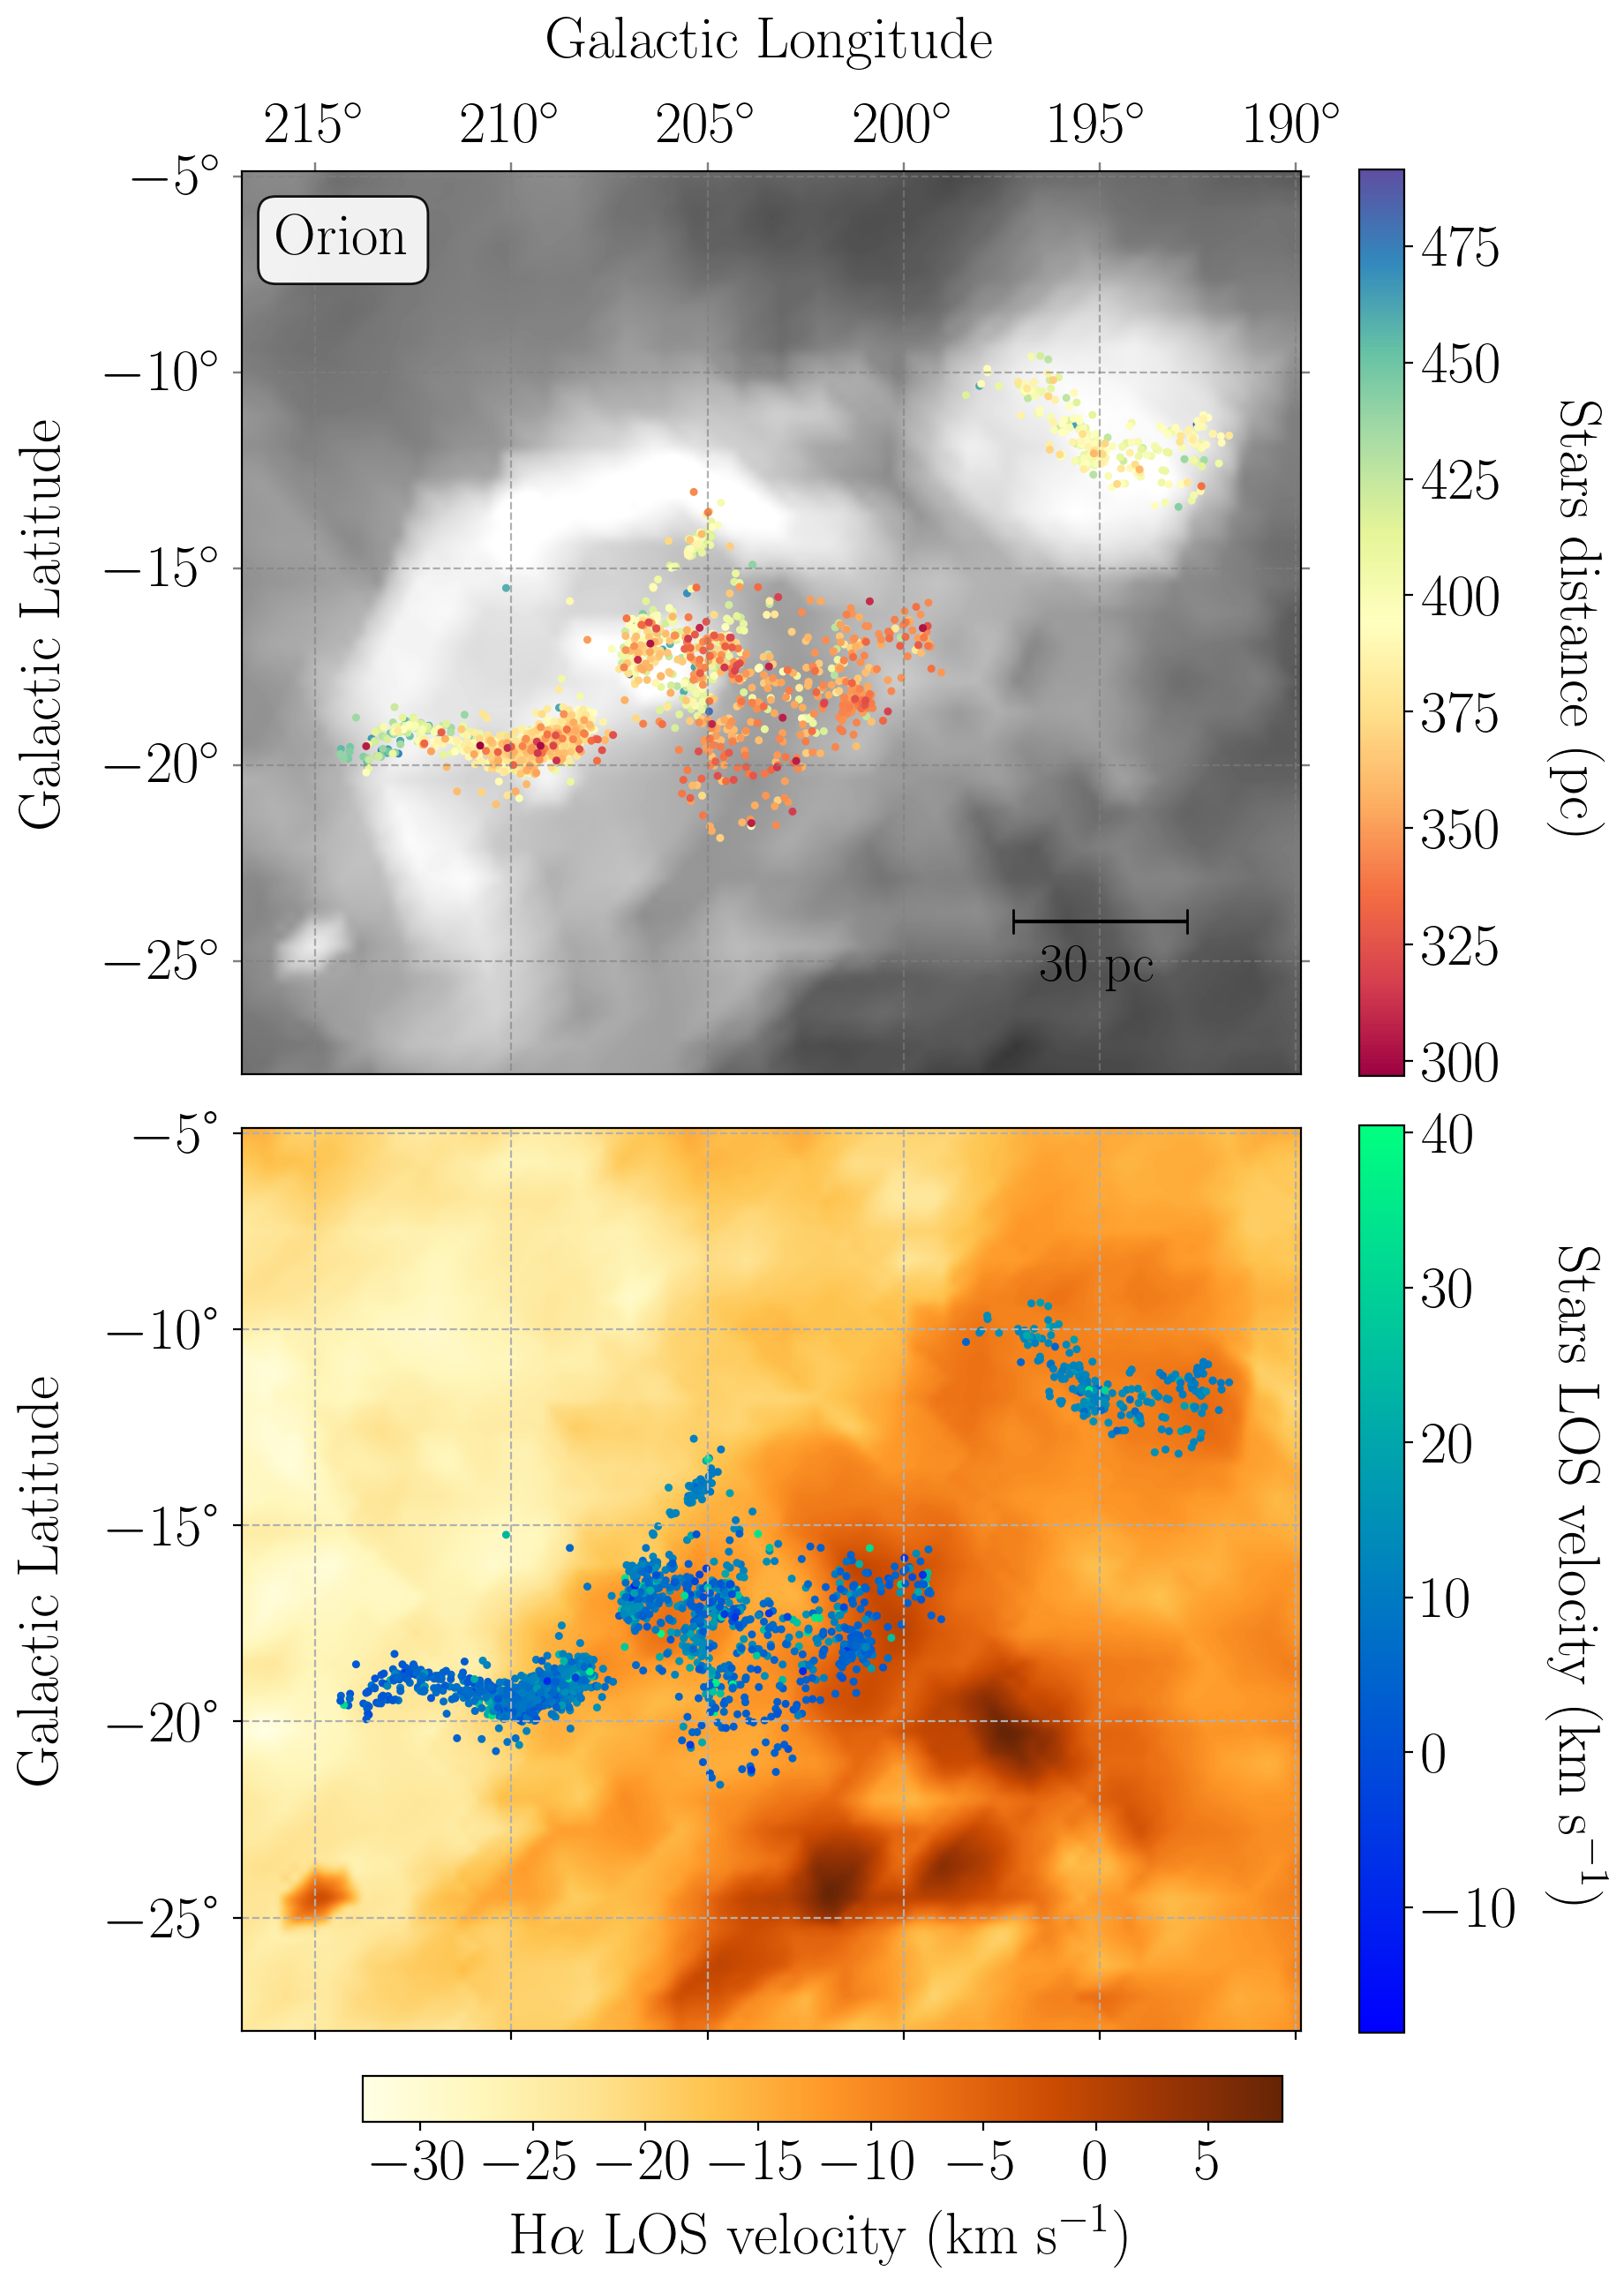
\includegraphics[width=0.37\linewidth,trim=0cm 0cm 0cm 0.2cm, clip=true]{Stars_img/Ori_fig1.png}
    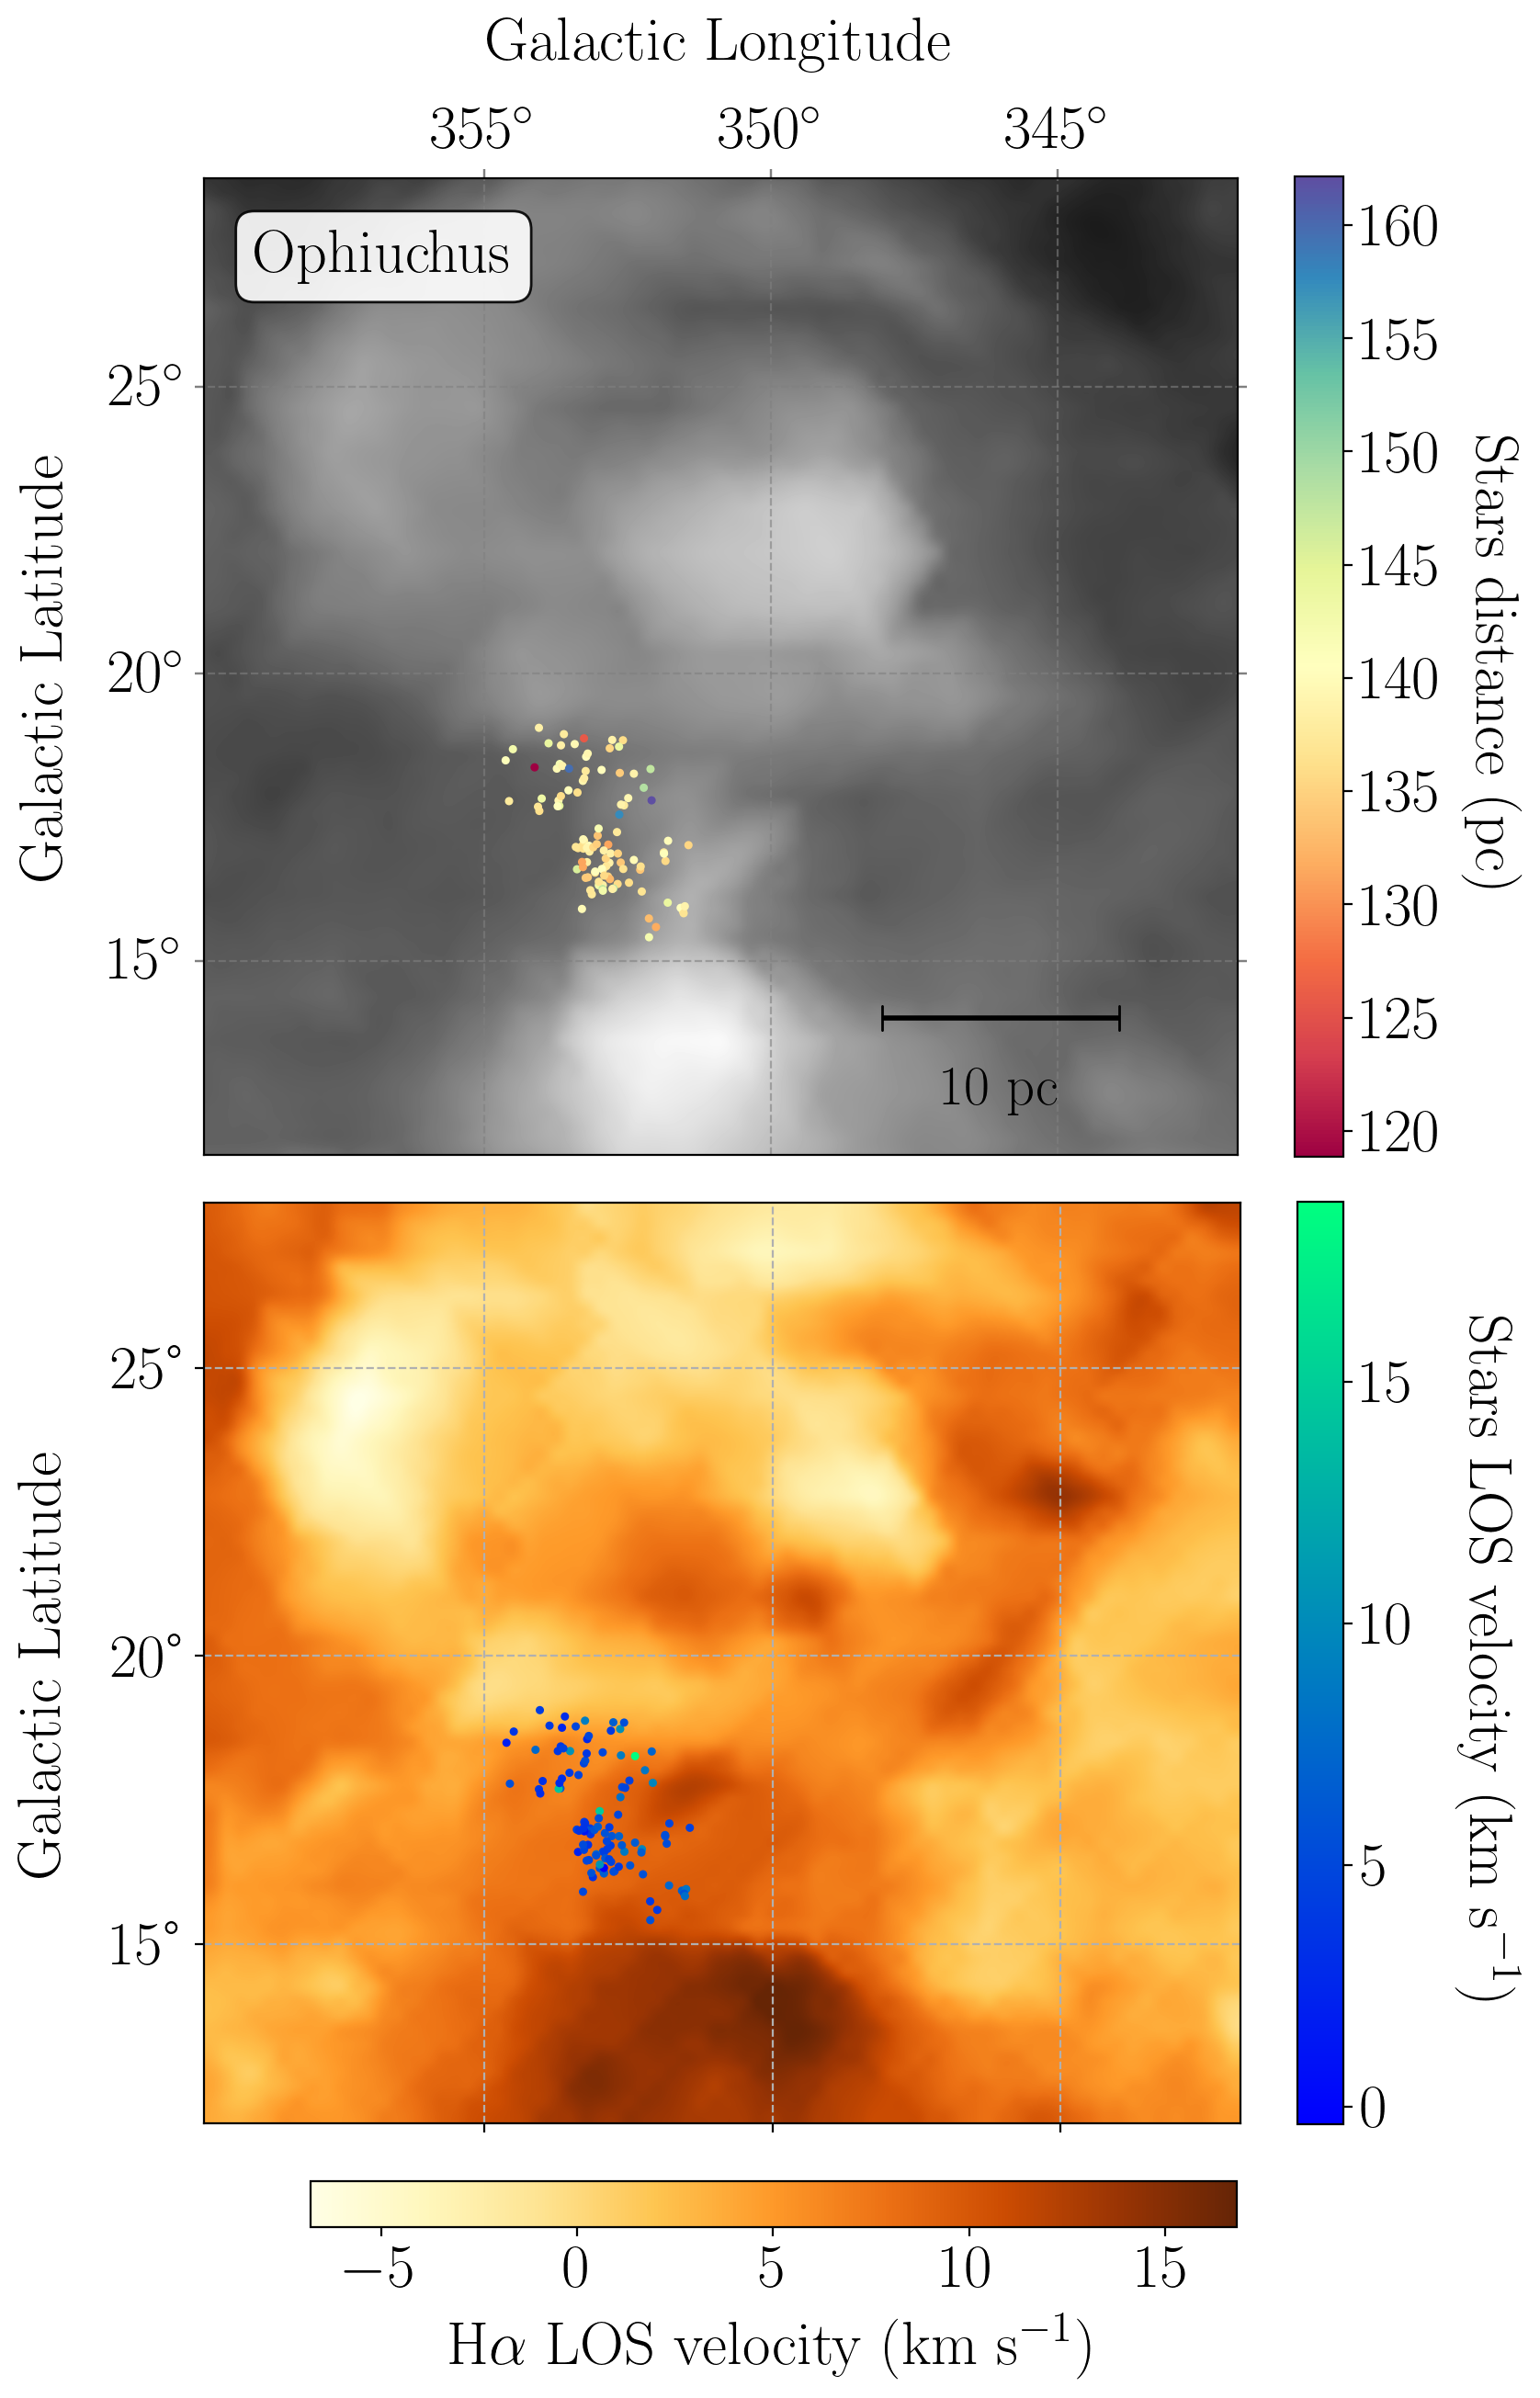
\includegraphics[width=0.312\linewidth,trim=1.5cm 0cm 0cm 0.1cm, clip=true]{Stars_img/Ophi_fig1.png}
    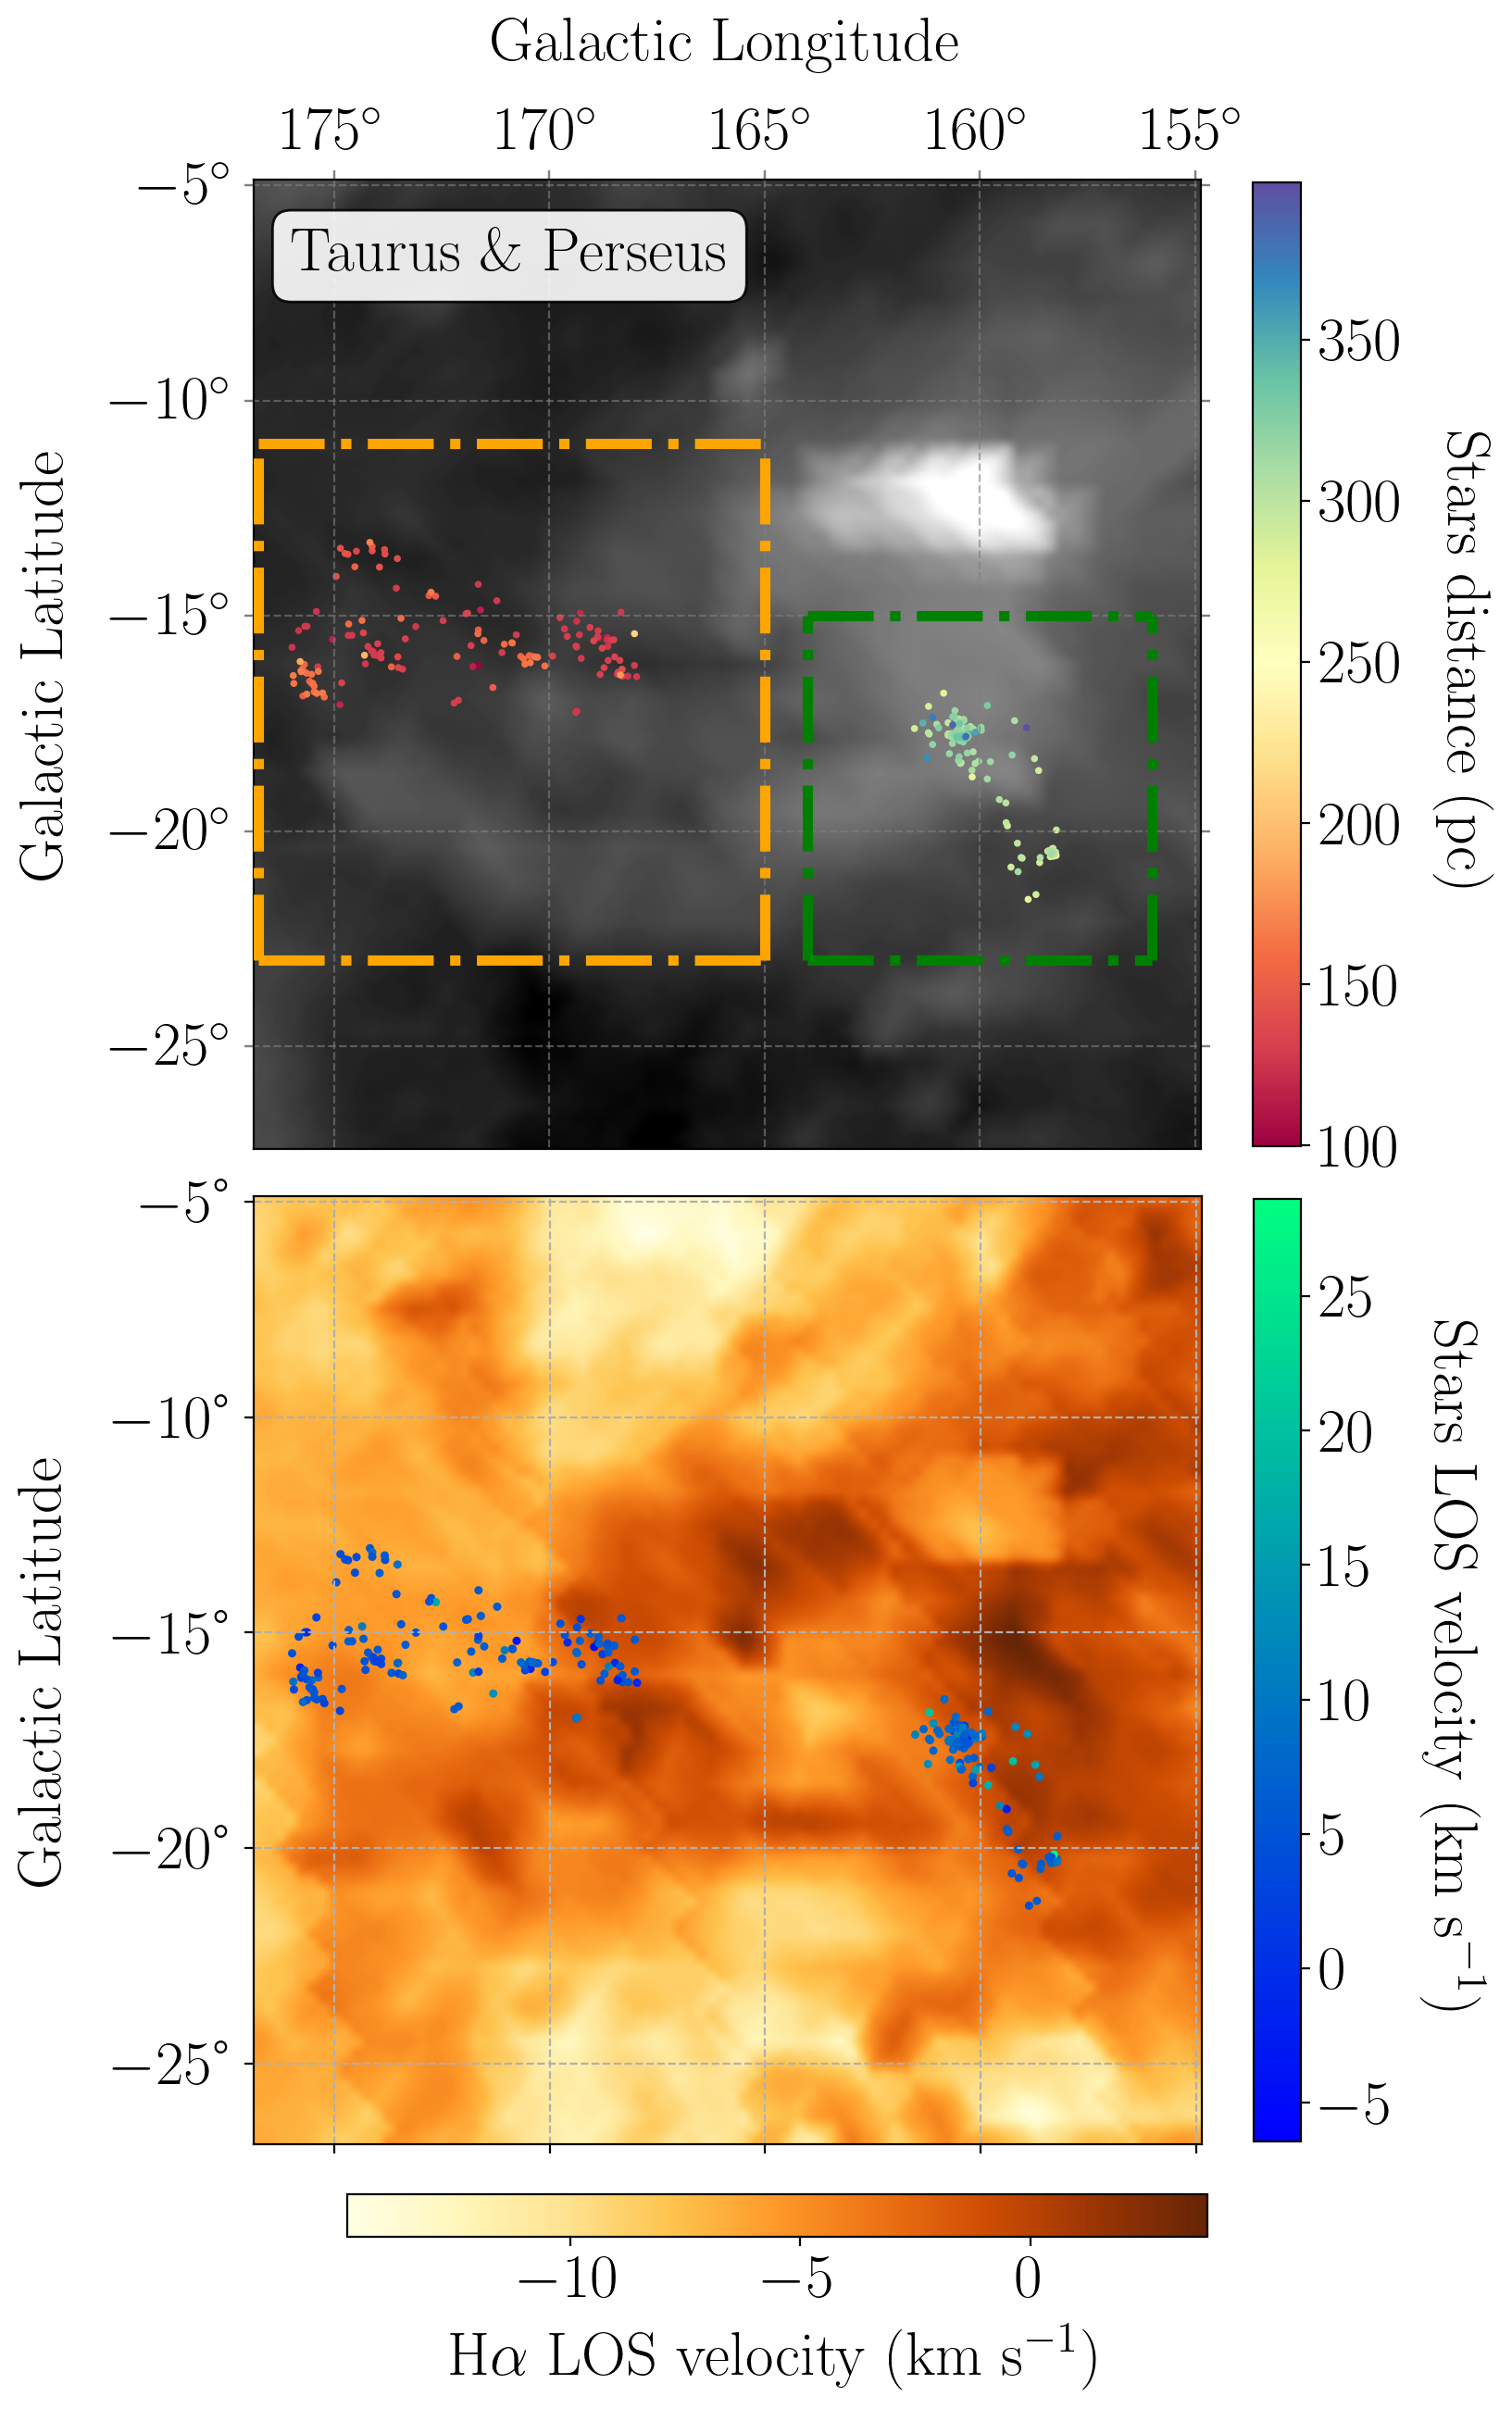
\includegraphics[width=0.302\linewidth,trim=1.6cm 0cm 0.1cm 0.1cm, clip=true]{Stars_img/PerTau_fig1.png}
    \caption{Top panels: positions of young stars color-coded by their distances in Orion, Ophiuchus, Taurus-Perseus (from left to right). Background shows \halpha~flux from the WHAM survey (lighter is brighter). 
    The orange and green boxes denote the areas where \halpha~is analyzed for Taurus and Perseus, respectively.
    Bottom panels show the line-of-sight velocities of the young stars (in the LSR frame) in these regions. The background shows the \halpha~line-of-sight centroid velocities.}
    \label{fig:allsky}
\end{figure*}


\begin{sidewaystable}
    \centering
    \caption{Properties of Star-Forming Regions}
    \label{tab:properties}
    \begin{tabular}{ccccccccc}
        \toprule
        Region        &
        Number of     &
        Number of     &
        Average       &
        GLON          &
        GLAT          &
        Distance      &
        $v_{\rm LSR}$ range          &
        $v_{\rm LSR,~err}$ cut       \\
                      &
        stars         &
        stars used    &
        distance (pc) &
        (\textdegree) &
        (\textdegree) &
        range (pc)    &
        ($\mathrm{km~s^{-1}}$)       &
        ($\mathrm{km~s^{-1}}$)       \\
        \midrule
        Orion     & 2647 & 2468 & 410 & $190,217$ & $-28,-5$  & $300,500$ & $-10,40$ & $10$ \\
        Ophiuchus & 113  & 107  & 140 & $342,360$ & $12,28$   & $120,170$ & $-30,30$ & $2$  \\
        Perseus   & 159  & 138  & 320 & $156,164$ & $-23,-15$ & $250,400$ & $-6,30$  & $10$ \\
        Taurus    & 157  & 139  & 140 & $165,177$ & $-23,-11$ & $97,200$  & $-5,25$  & $5$  \\
        \bottomrule
    \end{tabular}
    \parbox{\linewidth}{\footnotesize \textit{Note.} Number of stars are all 
    the stars with 6D information. Number of stars used are the stars in our 
    analysis after excluding outliers. GLON (Galactic Longitude) and GLAT 
    (Galactic Latitude) ranges denote the borders of windows used to compute 
    the \halpha~VSF\@. The distance ranges, $v_{\rm LSR}$~ranges, and
    $v_{\rm LSR,~err}$~cuts are applied to the stars to exclude outliers.}
\end{sidewaystable}

\subsection{Observations, Data reduction, and Methods} \label{sec:data_method}
\subsubsection{Observations and Data Analysis} \label{sec:alldata}

\centerline{\textbf{Stellar observations}}

We obtain the locations, parallax distances, and proper motions of stars from the Gaia mission \citep{collaboration_gaia_2016} in four nearby star-forming regions: the Orion Molecular Cloud complex (Orion), the \rophi~dark cloud (Ophiuchus), the Perseus molecular cloud traced by two clusters, NGC 1333 and IC 348 (Perseus), and the Taurus molecular clouds (Taurus). The Gaia catalog includes five-parameter astrometric measurements (plane-of-sky coordinates, proper motions, and parallax distances) of over 1.46 billion stars in the Milky Way. Only a very limited subset ($\sim 7$ million) has line-of-sight velocities measured by Gaia. The five-dimensional astrometric data for our four regions are obtained from Gaia's third early data release \citep[EDR3;][]{brown_gaia_2021}. 

The line-of-sight velocities of the stars in our study were observed in the near infrared with the Apache Point Observatory Galactic Evolution Experiment (APOGEE) spectrograph, mounted on the 2.5 m Sloan Foundation Telescope of the Sloan Digital Sky Survey. APOGEE-2 Data Release 17 (DR17) collected high resolution spectral image of over 657,000 stars in the Milky Way \citep{gunn_25_2006,blanton_sloan_2017,abdurrouf_seventeenth_2022}. Combining these two surveys provides six-dimensional (6D) information (3D positions and 3D velocities) of stars for the four molecular clouds.

The stars in our study were assigned to each of the four region by \citet{kounkel_untangling_2019}. They performed a clustering analysis on Gaia DR2 sources in the Milky Way using Python implementation of HDBSCAN \citep[Hierarchical Density-Based Spatial Clustering of Applications with Noise;][]{mcinnes_hdbscan_2017}. We crossmatch this catalog with Gaia EDR3 and APOGEE-2 to obtain 6D astrometries of the stars. 

Then, we exclude a small number of stars whose parallax distances $d$, line-of-sight velocities $v_{\rm LSR}$, and line-of-sight velocity errors $v_{\rm LSR,~err}$~are more than 4$\sigma$~deviated from the mean of the distribution. In Taurus, one star with very high reported proper motion ($v_{\rm LSR,~RA} > 100\mathrm{~mas~yr}^{-1}$) is excluded.
The ranges of $d$~and $v_{\rm LSR}$, and the threshold of $v_{\rm LSR,~err}$~that we use, as well as the total number of stars before and after the cut are specified in Table \ref{tab:properties}. We note, however, that the exact cut of these ranges do not affect the conclusion of this work.

\centerline{\textbf{\halpha~observations}}

The \halpha~data in our study comes from the WHAM survey \citep[][]{haffner_wisconsin_2003,haffner_early_2010}. We obtained the data cubes from the ``DR1-v161116-170912" release, which comprises more than 49000 spectra divided into an irregular grid with a spatial resolution of 1\textdegree, and the data cube is Nyquist-sampled with $4\times4$~pixels per resolution element \citep[][]{haffner_wisconsin_2003}. The intensity of the \halpha~emission is recorded in a 3-dimensional array encoding its Galactic longitude, Galactic latitude, and line-of-sight velocity ($-170$ km s$^{-1} < v_{\rm LSR} < 160$ km s$^{-1}$). We fit a Gaussian distribution to the flux profile along individual lines of sight. Then we take the velocity at the peak of the distribution as the centroid velocity and the uncertainty of the fit as the uncertainty. We also correct for Galactic rotation following the procedure in \citet{qu_warm_2020}.

Figure \ref{fig:allsky} shows the \halpha~map of the four regions in our analysis, with stars overplotted as foreground dots. The top panels show the integrated line-of-sight fluxes in log scale. In the foreground, each star is color-coded by their distance from Earth. We note that although Perseus and Taurus are very close to each other on the sky, they are physically separated by $\sim 150$~pc along the line of sight. In the bottom panels, we plot the centroid velocity of the \halpha~in the background, and the line-of-sight velocities of stars in the foreground.

\subsubsection{Data analysis} \label{sec:analysis}

We compute the first-order VSF of stars in each region. The VSF is related to the kinetic energy power spectrum of a velocity field, and is expressed as a two-point correlation function between the absolute velocity differences $|\delta v|$ versus the physical separation $\ell$. For a turbulent velocity field, we expect the VSF to have a characteristic power-law scaling with slope 1/3 for incompressible turbulence dominated by solenoidal motions \citep[][]{kolmogorov_local_1941}, or a slope 1/2 for supersonic turbulence dominated by compressive motions. For the Milky Way molecular clouds, \citet{larson_turbulence_1981} found a relationship between cloud size and velocity dispersion to be $\sigma = 1.1~R^{0.38}$.

The 3D VSF of stars is computed as follows. First, the positions, distances, radial velocities, and proper motions of stars are translated into galactocentric Cartesian coordinates and velocities. Then, for each pair of stars, the absolute velocity vector difference $|\delta \vec v|$ and the distance $d$ between them is calculated. For individual clouds, these distances are sorted into logarithmic bins of $\ell$, and $|\delta \vec v|$ values within a bin are averaged out to obtain \vsf. To estimate uncertainties, we first generate 1000 random samples of stellar parameters following a Gaussian distribution around the reported measurements and with a 1$\sigma$ scatter equal to the reported uncertainties. Then at each $\ell$, we take the 1$\sigma$ value of the 1000 \vsf~to be the uncertainty.

For the WHAM \halpha~data, we first define a rectangular box containing the stars in each of the four regions as specified in Table \ref{tab:properties} and shown in Figure~\ref{fig:allsky}. Our results are not sensitive to the exact size of the box (see Section \ref{sec:windowsize} for detailed discussions). We compute the first-order VSF of each region using the projected position-position-velocity information. The resultant VSF is $\langle |\delta v| \rangle_{\rm proj}$~versus angular separations $\theta$. Then, we assume a constant distance equal to the mean distance of stars in each region (see Table~\ref{tab:properties}) and translate $\theta$~(\textdegree) to $\ell_{\rm proj}$~(pc). Since three degrees of freedom are missing in this projected VSF calculation (the proper motions of gas and its exact distance), we scale $\langle |\delta v| \rangle_{\rm proj}$~and $\ell_{\rm proj}$ by a constant factor, assuming an isotropic turbulent velocity field. 

\begin{equation}
    \langle|\delta \vec v|\rangle = \sqrt{3}~ \langle|\delta v|\rangle_{\rm proj},
\end{equation}
\begin{equation}
    \ell = \sqrt{\frac{3}{2}}~\ell_{\rm proj}.
\end{equation}

\subsection{Results} \label{sec:multi-region-results}

\begin{figure}
	\centering
	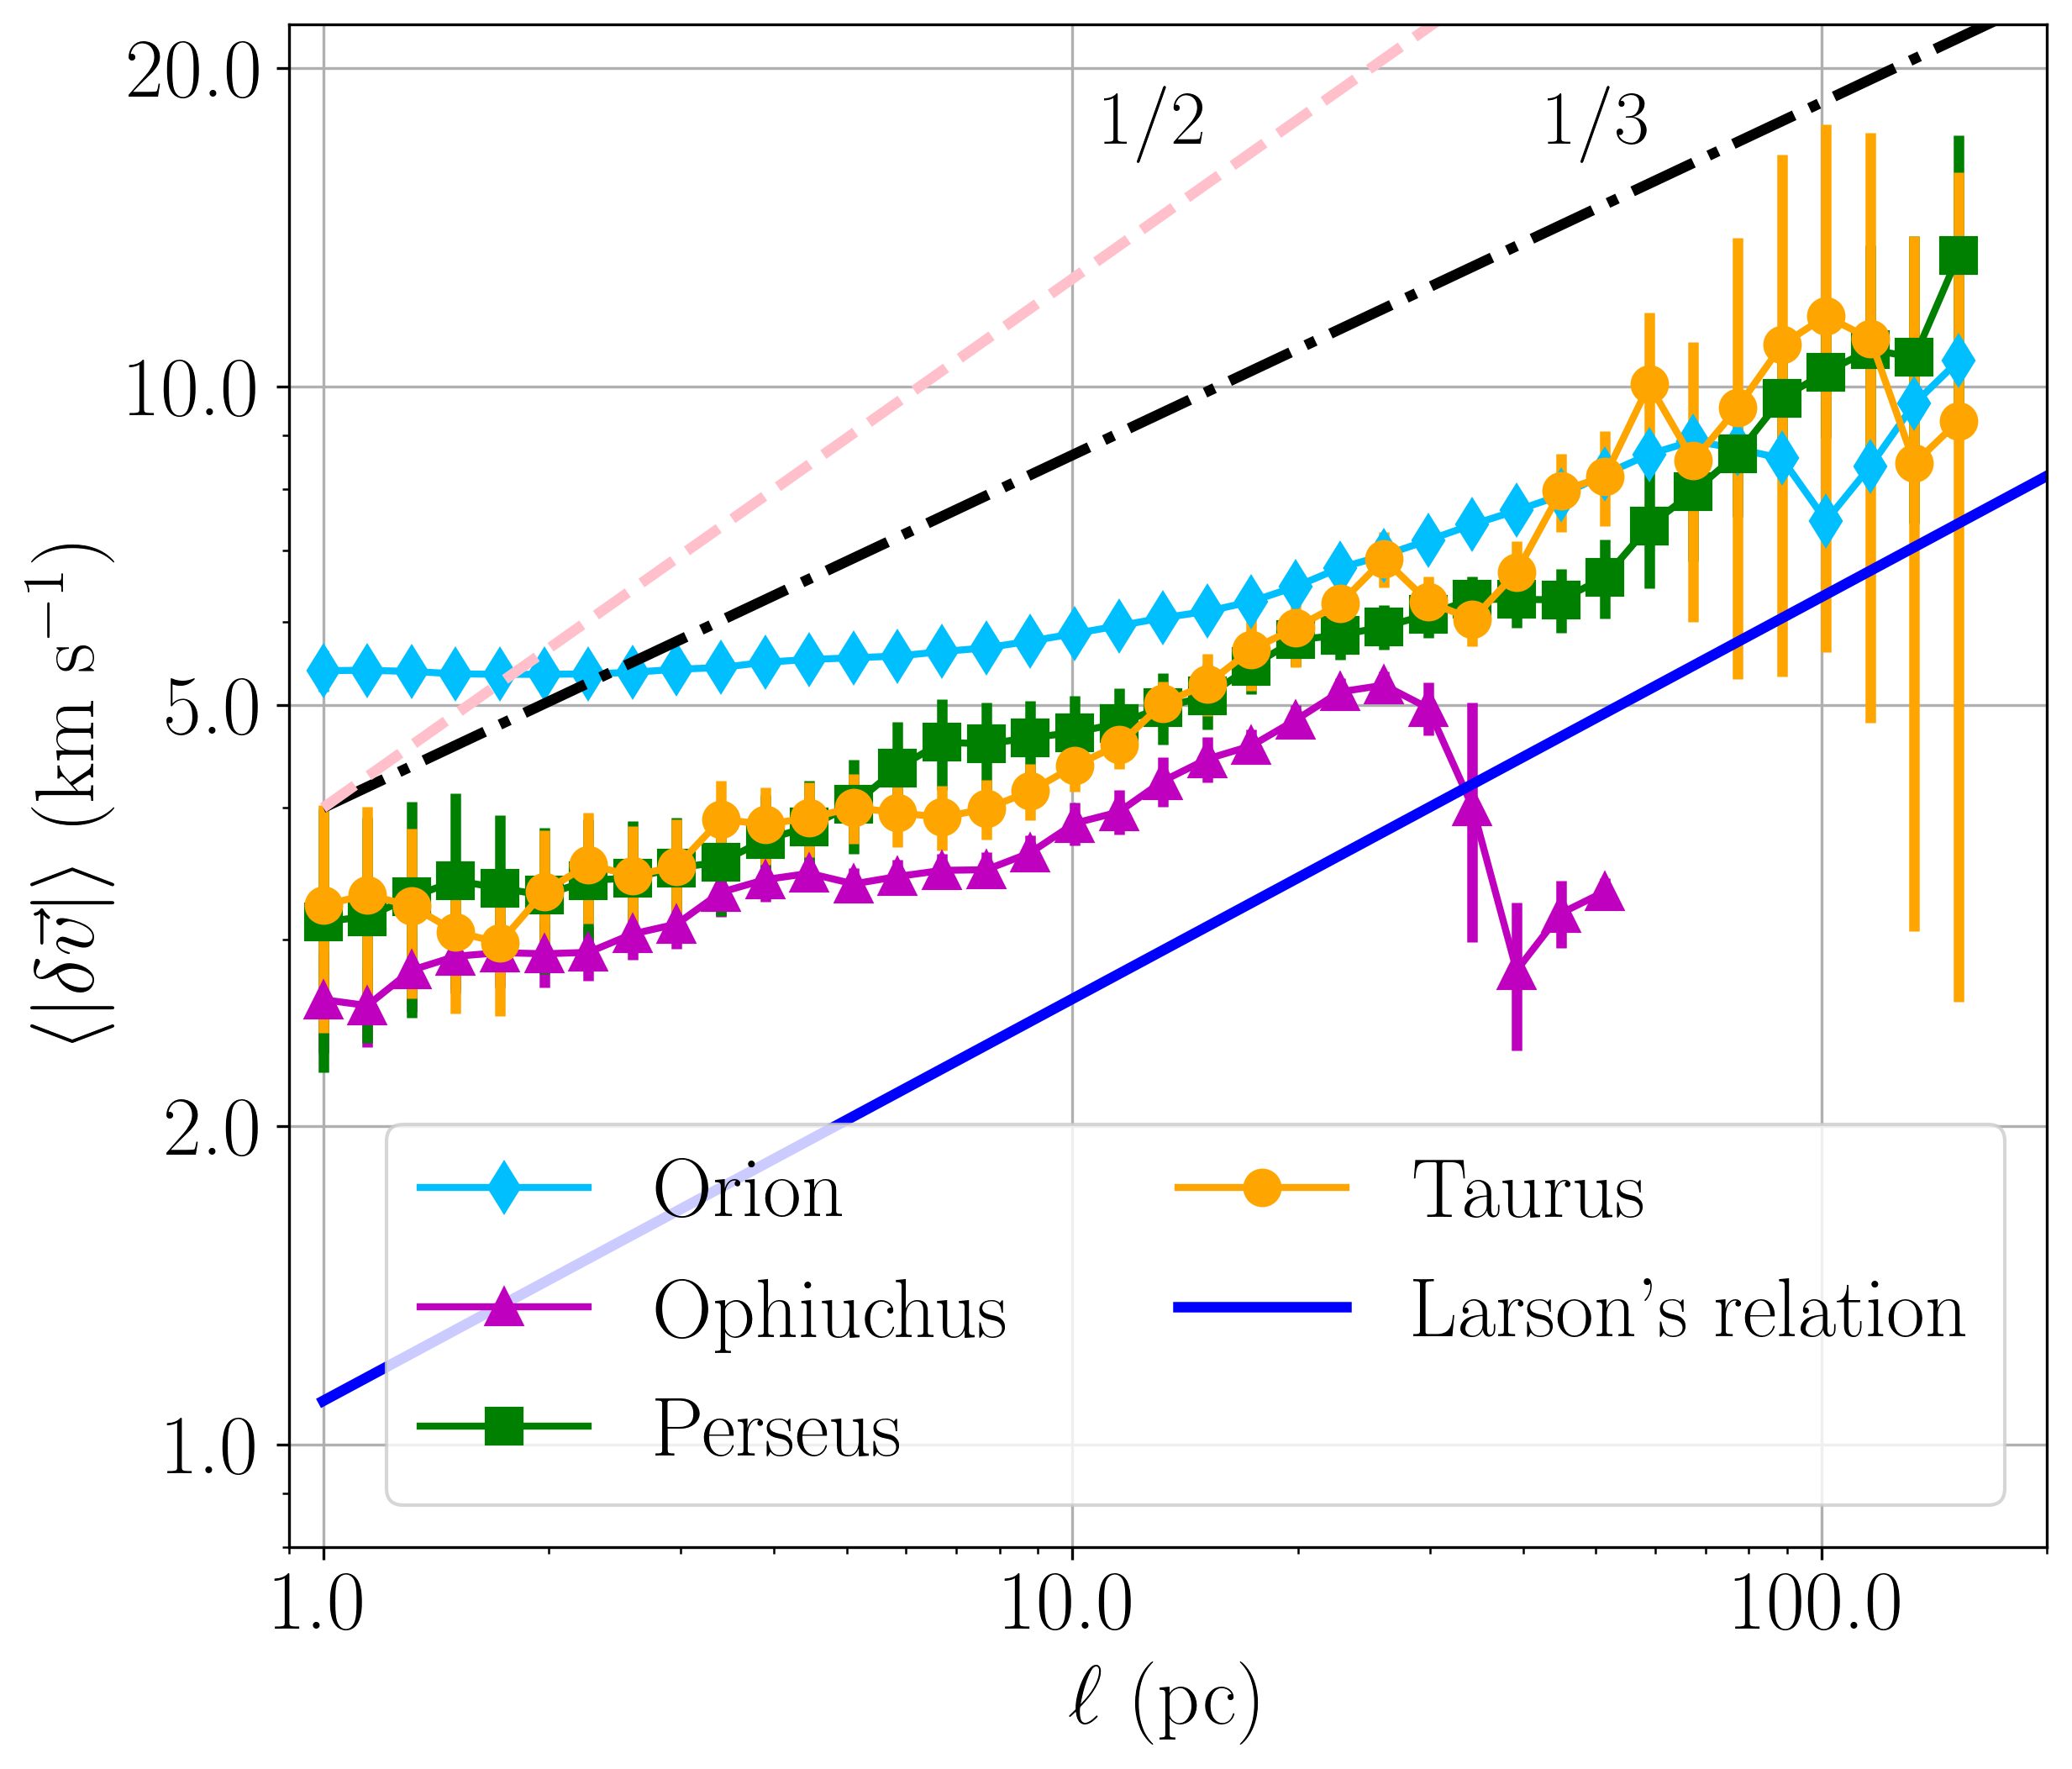
\includegraphics[width=\linewidth]{Stars_img/allstar_vsf_dr17.png}
	\caption{The first-order VSFs of the stars in Orion (light blue), Ophiuchus (magenta), Perseus (green), and Taurus (orange). For reference, we plot a solid blue line for Larson's relation, a black dotted-dashed line for Kolmogorov turbulence, and a pink dashed line for supersonic turbulence. The vertical lines represent the uncertainties in \vsf~ at each $\ell$.}
	\label{fig:starsvsf}
\end{figure}

\subsubsection{The Universality of ISM Turbulence Traced by Young Stars}\label{sec:starvsf}
We first examine the velocity statistics of the four star-forming regions: Orion, Ophiuchus, Perseus, and Taurus. Figure~\ref{fig:starsvsf} shows the VSFs traced by stars of these four regions. For reference, we also plot the Larson's relation of velocity dispersion vs. cloud size, the 1/3 slope of Kolmogorov turbulence, and the 1/2 slope of supersonic turbulence. Immediately, we recognize a remarkable universality among the VSFs of different regions. Over a large dynamical range, the magnitude and slopes of the VSFs show a general agreement with Larson's relation (see Table~\ref{tab:slopes} for the best-fit slopes of the VSFs). This suggests that the motion of young stars in the Milky Way show characteristics of turbulence, and supports our previous findings in Paper I that turbulence in the ISM can be traced with young stars.

At $\ell \lesssim 10$~pc, the slopes of the VSF of all four regions are flatter than Larson's relation, as well as Kolmogorov (slope 1/3) turbulence. We discuss the possible cause of this flattening in Section~\ref{sec:star_discussion}.

\subsubsection{The VSFs of Individual Regions} \label{subset:eachregion_result}

\begin{figure*}[ht!]
    \centering
    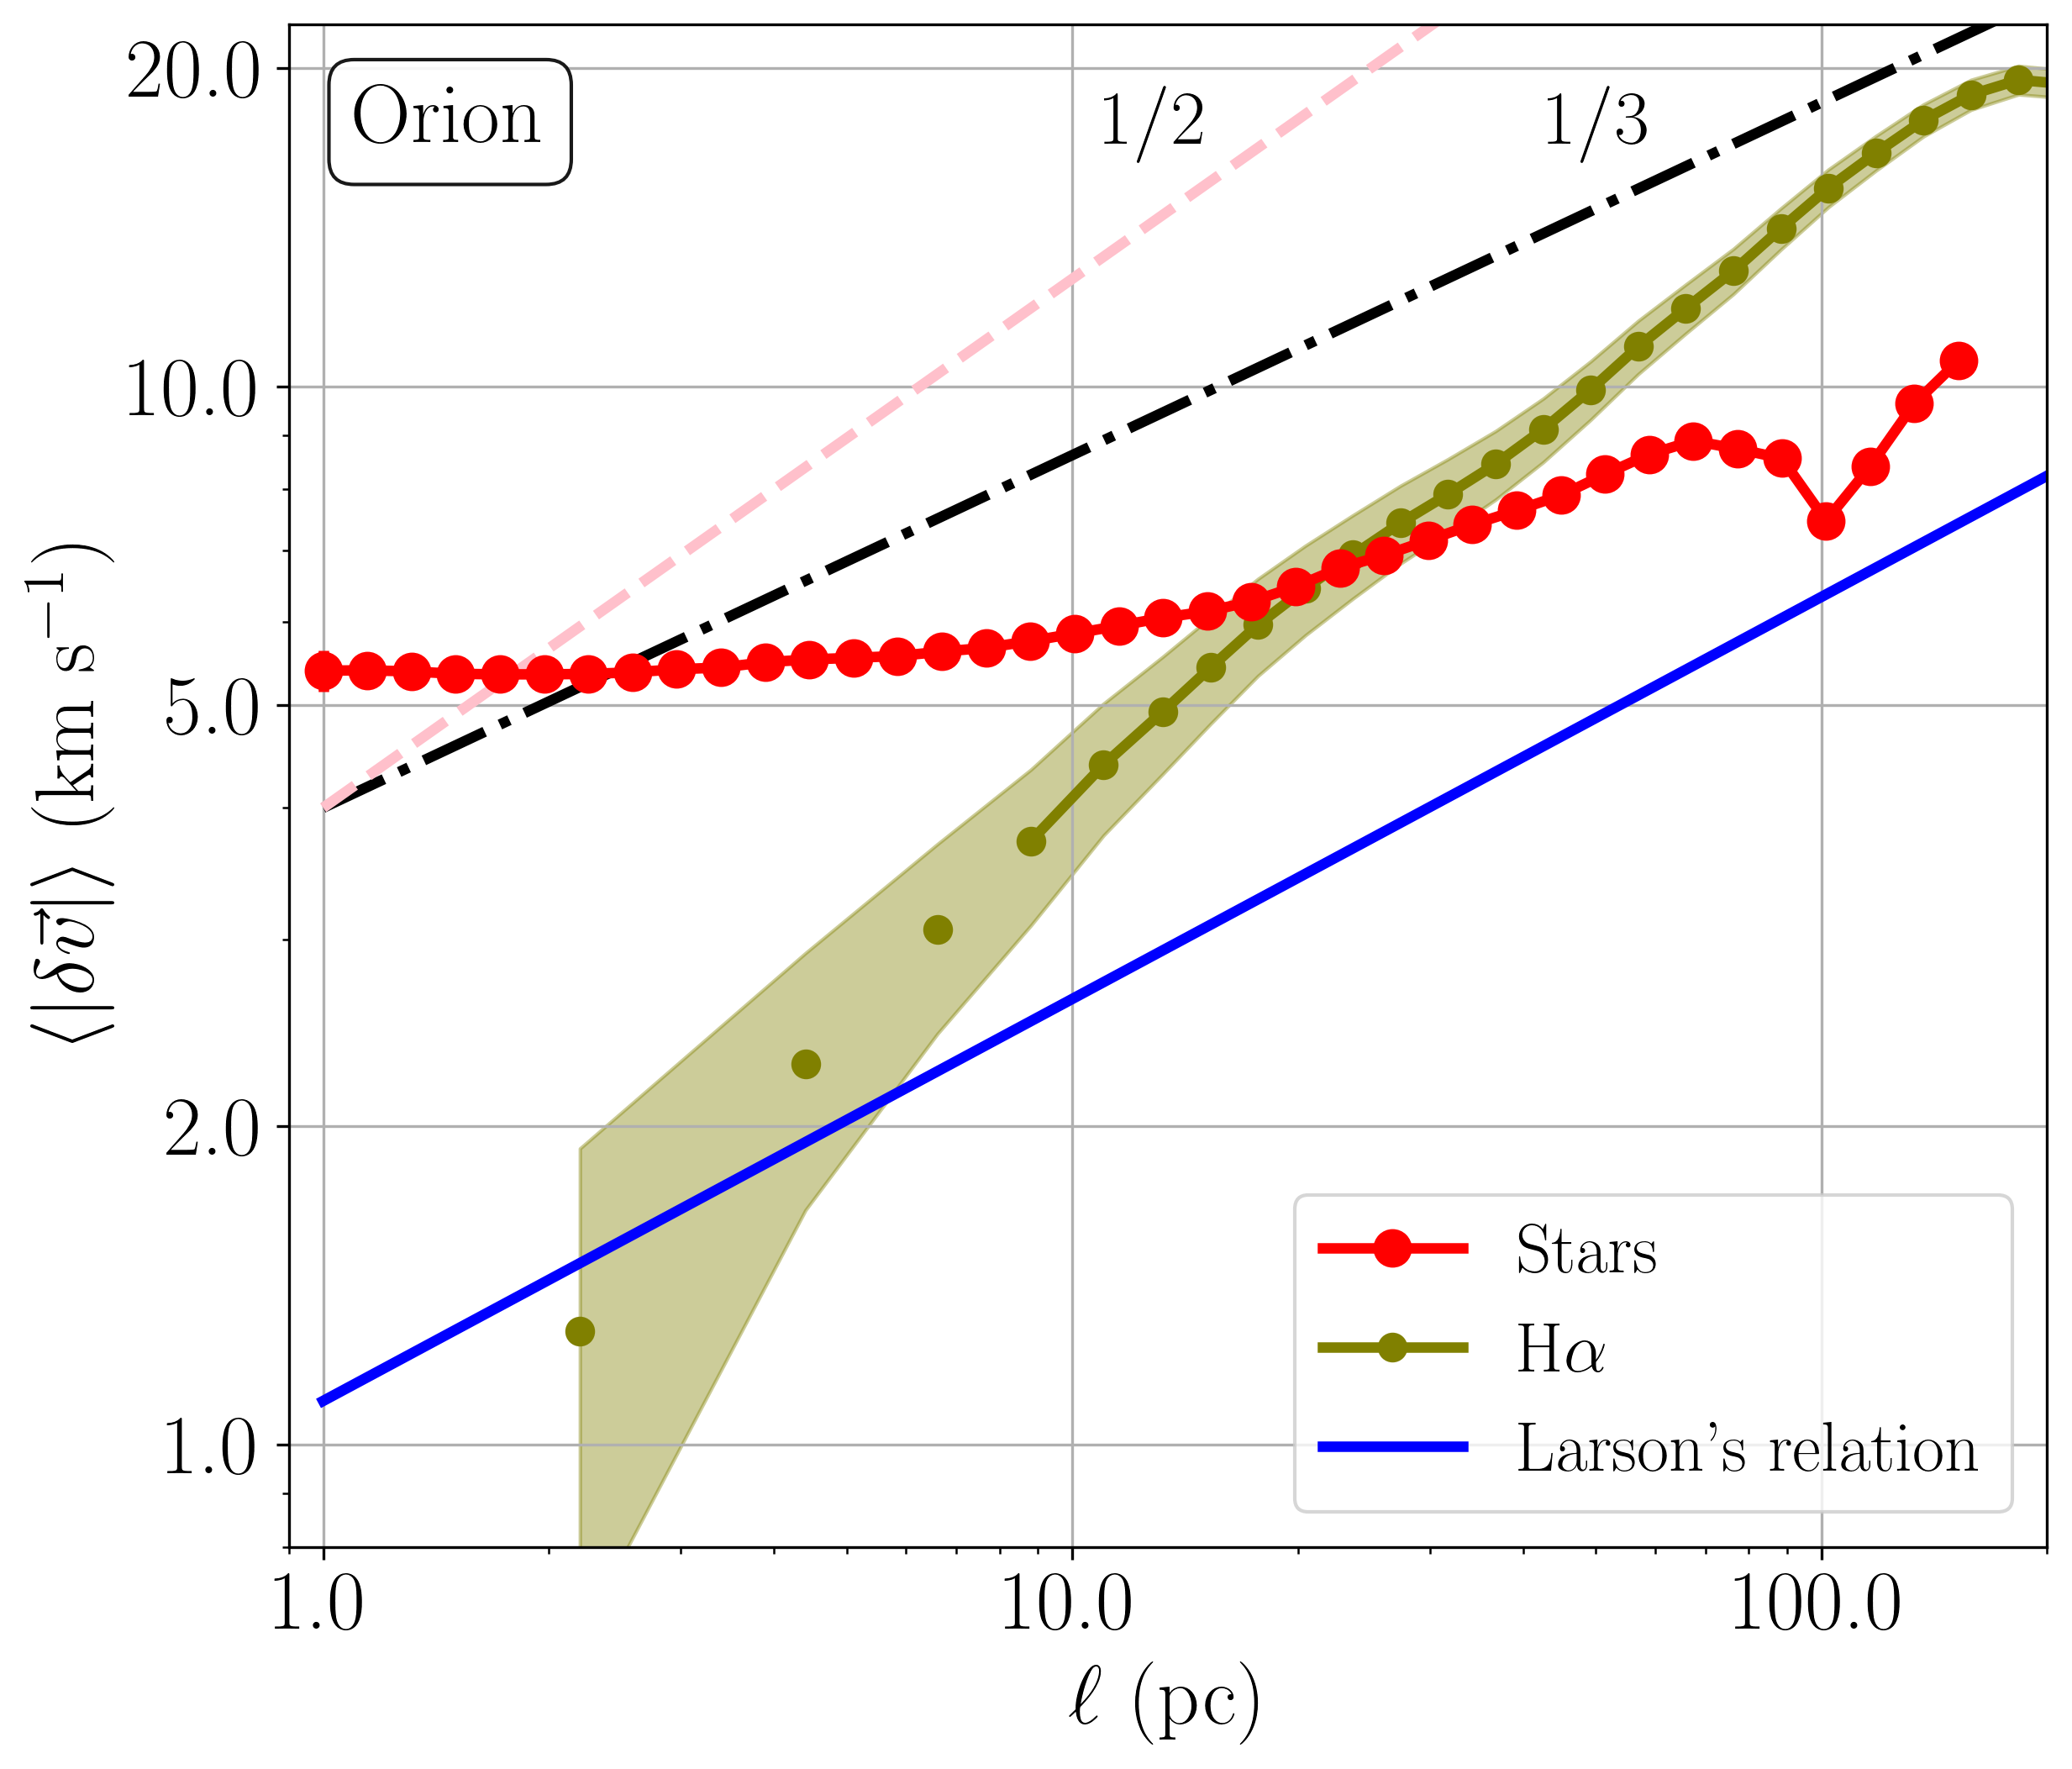
\includegraphics[width=0.48\linewidth]{Stars_img/Ori_fill.png}
    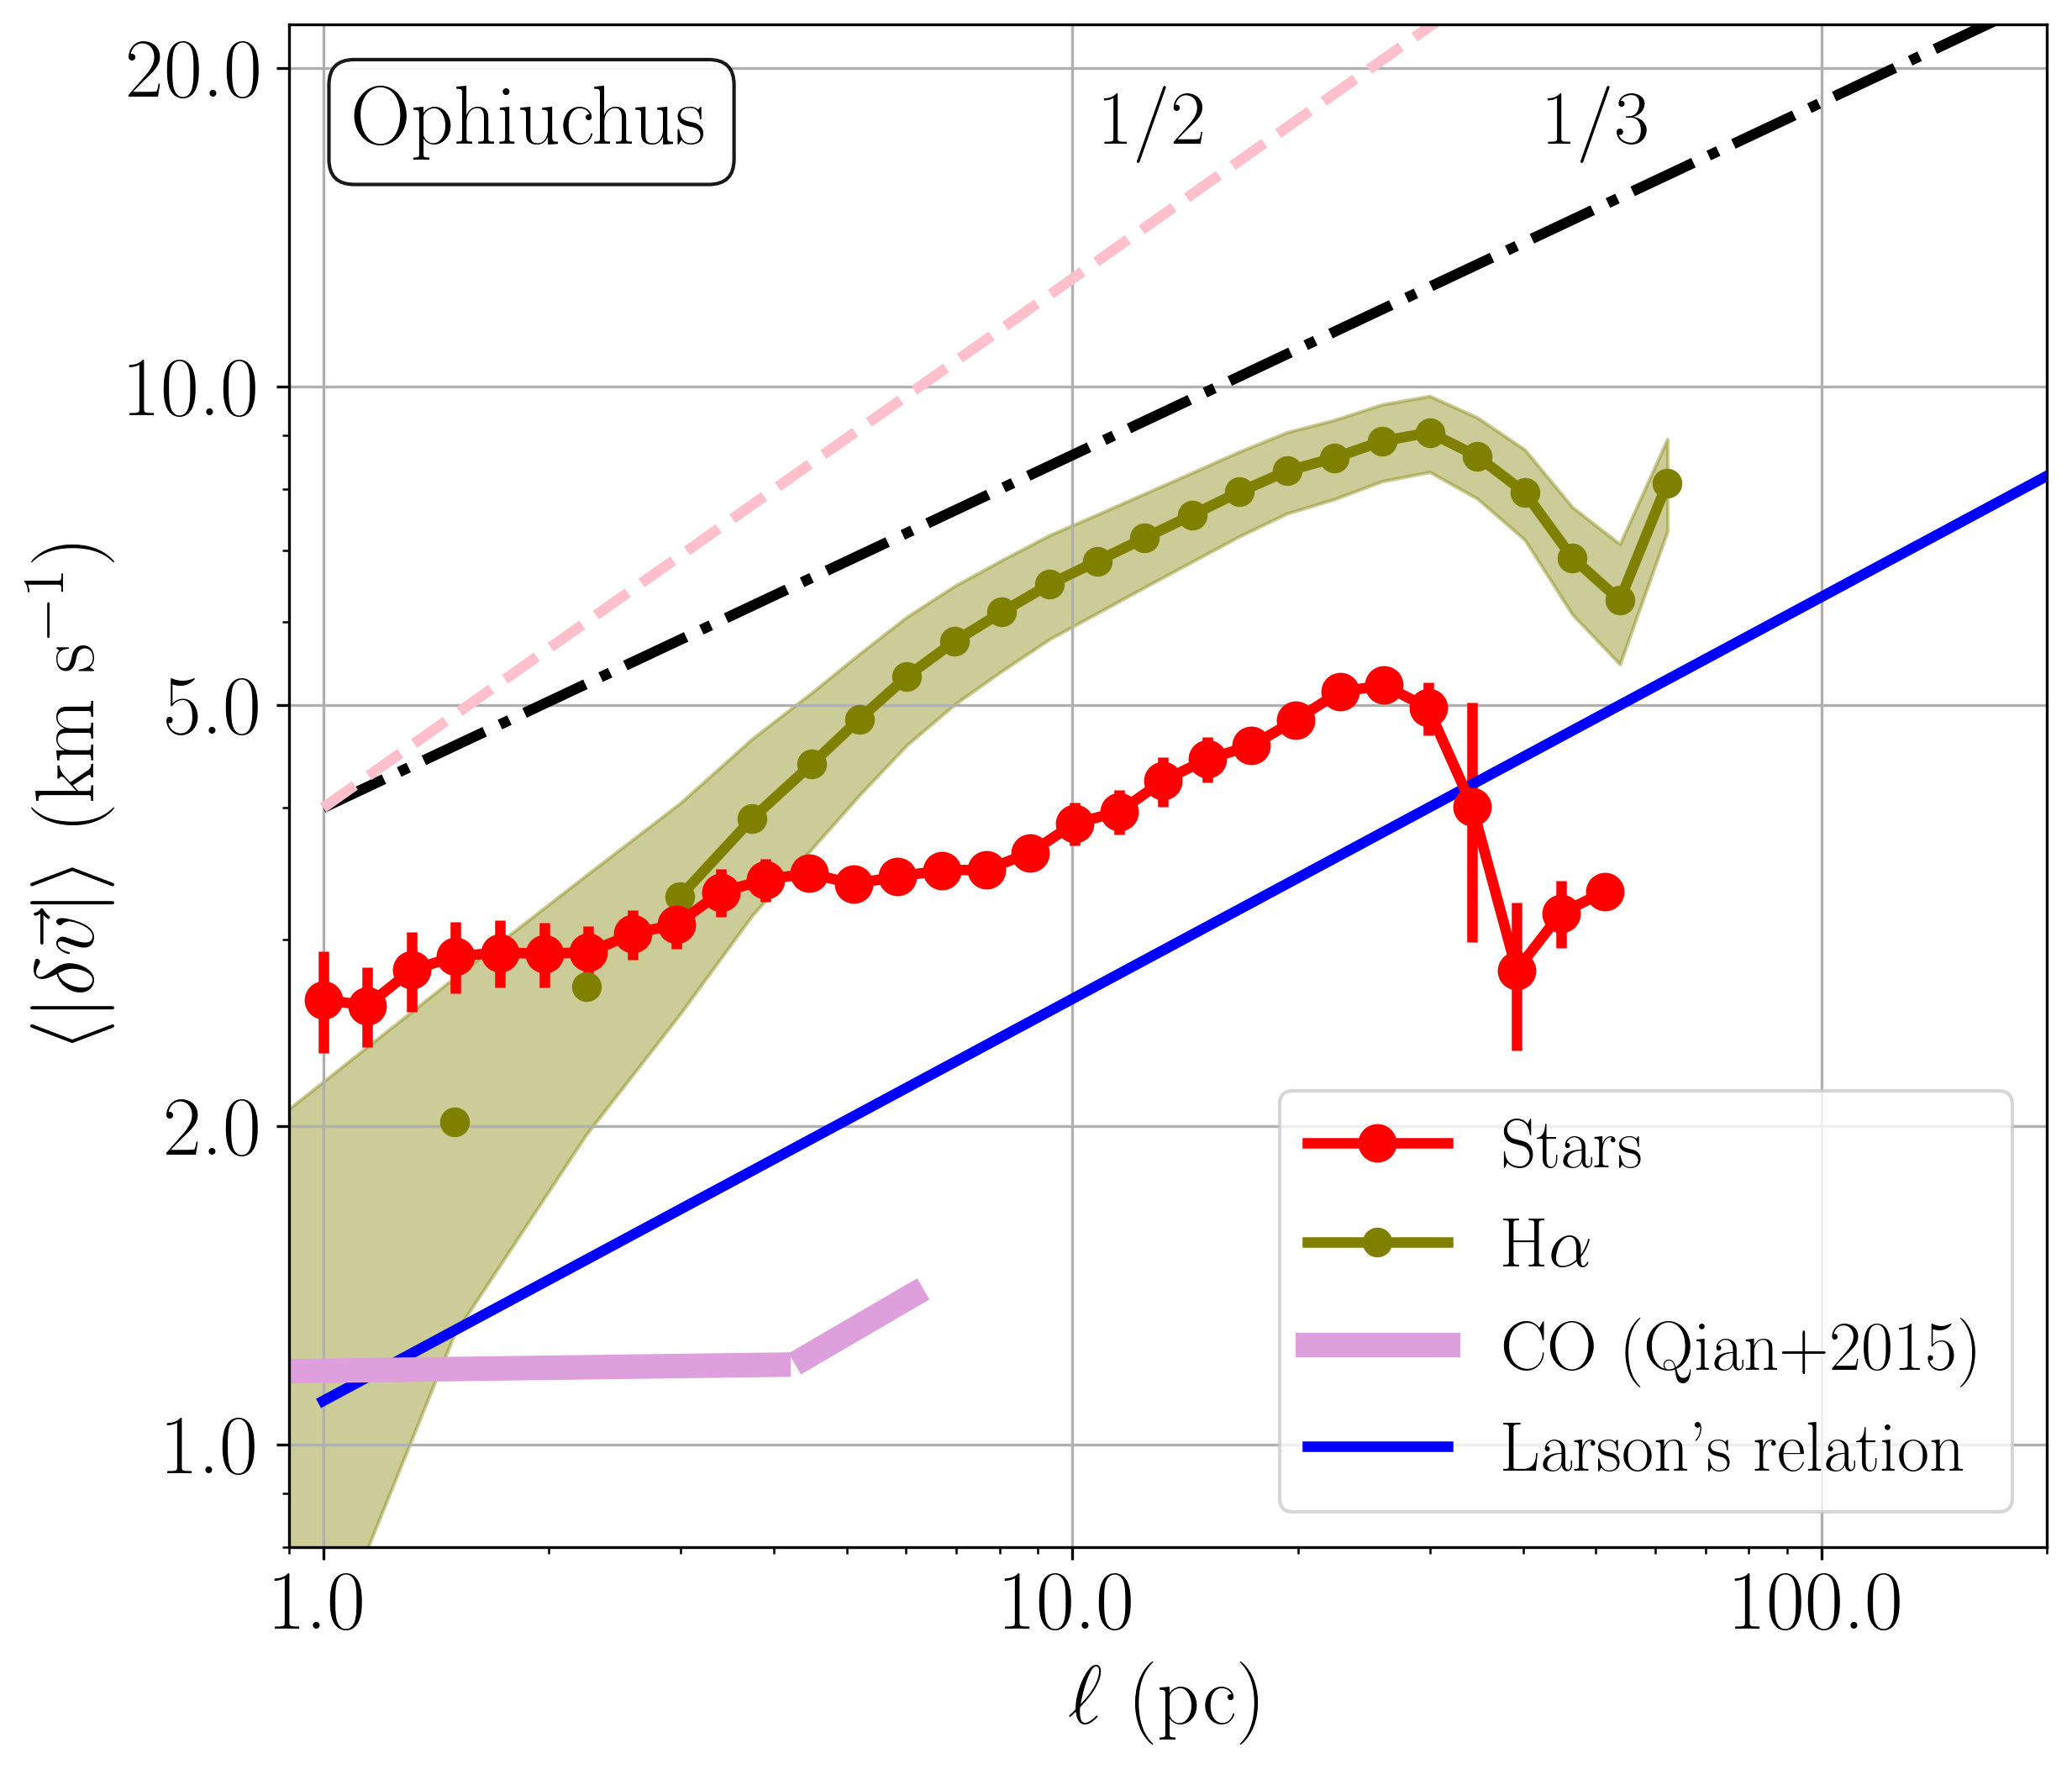
\includegraphics[width=0.48\linewidth]{Stars_img/Ophi_fill.png}
    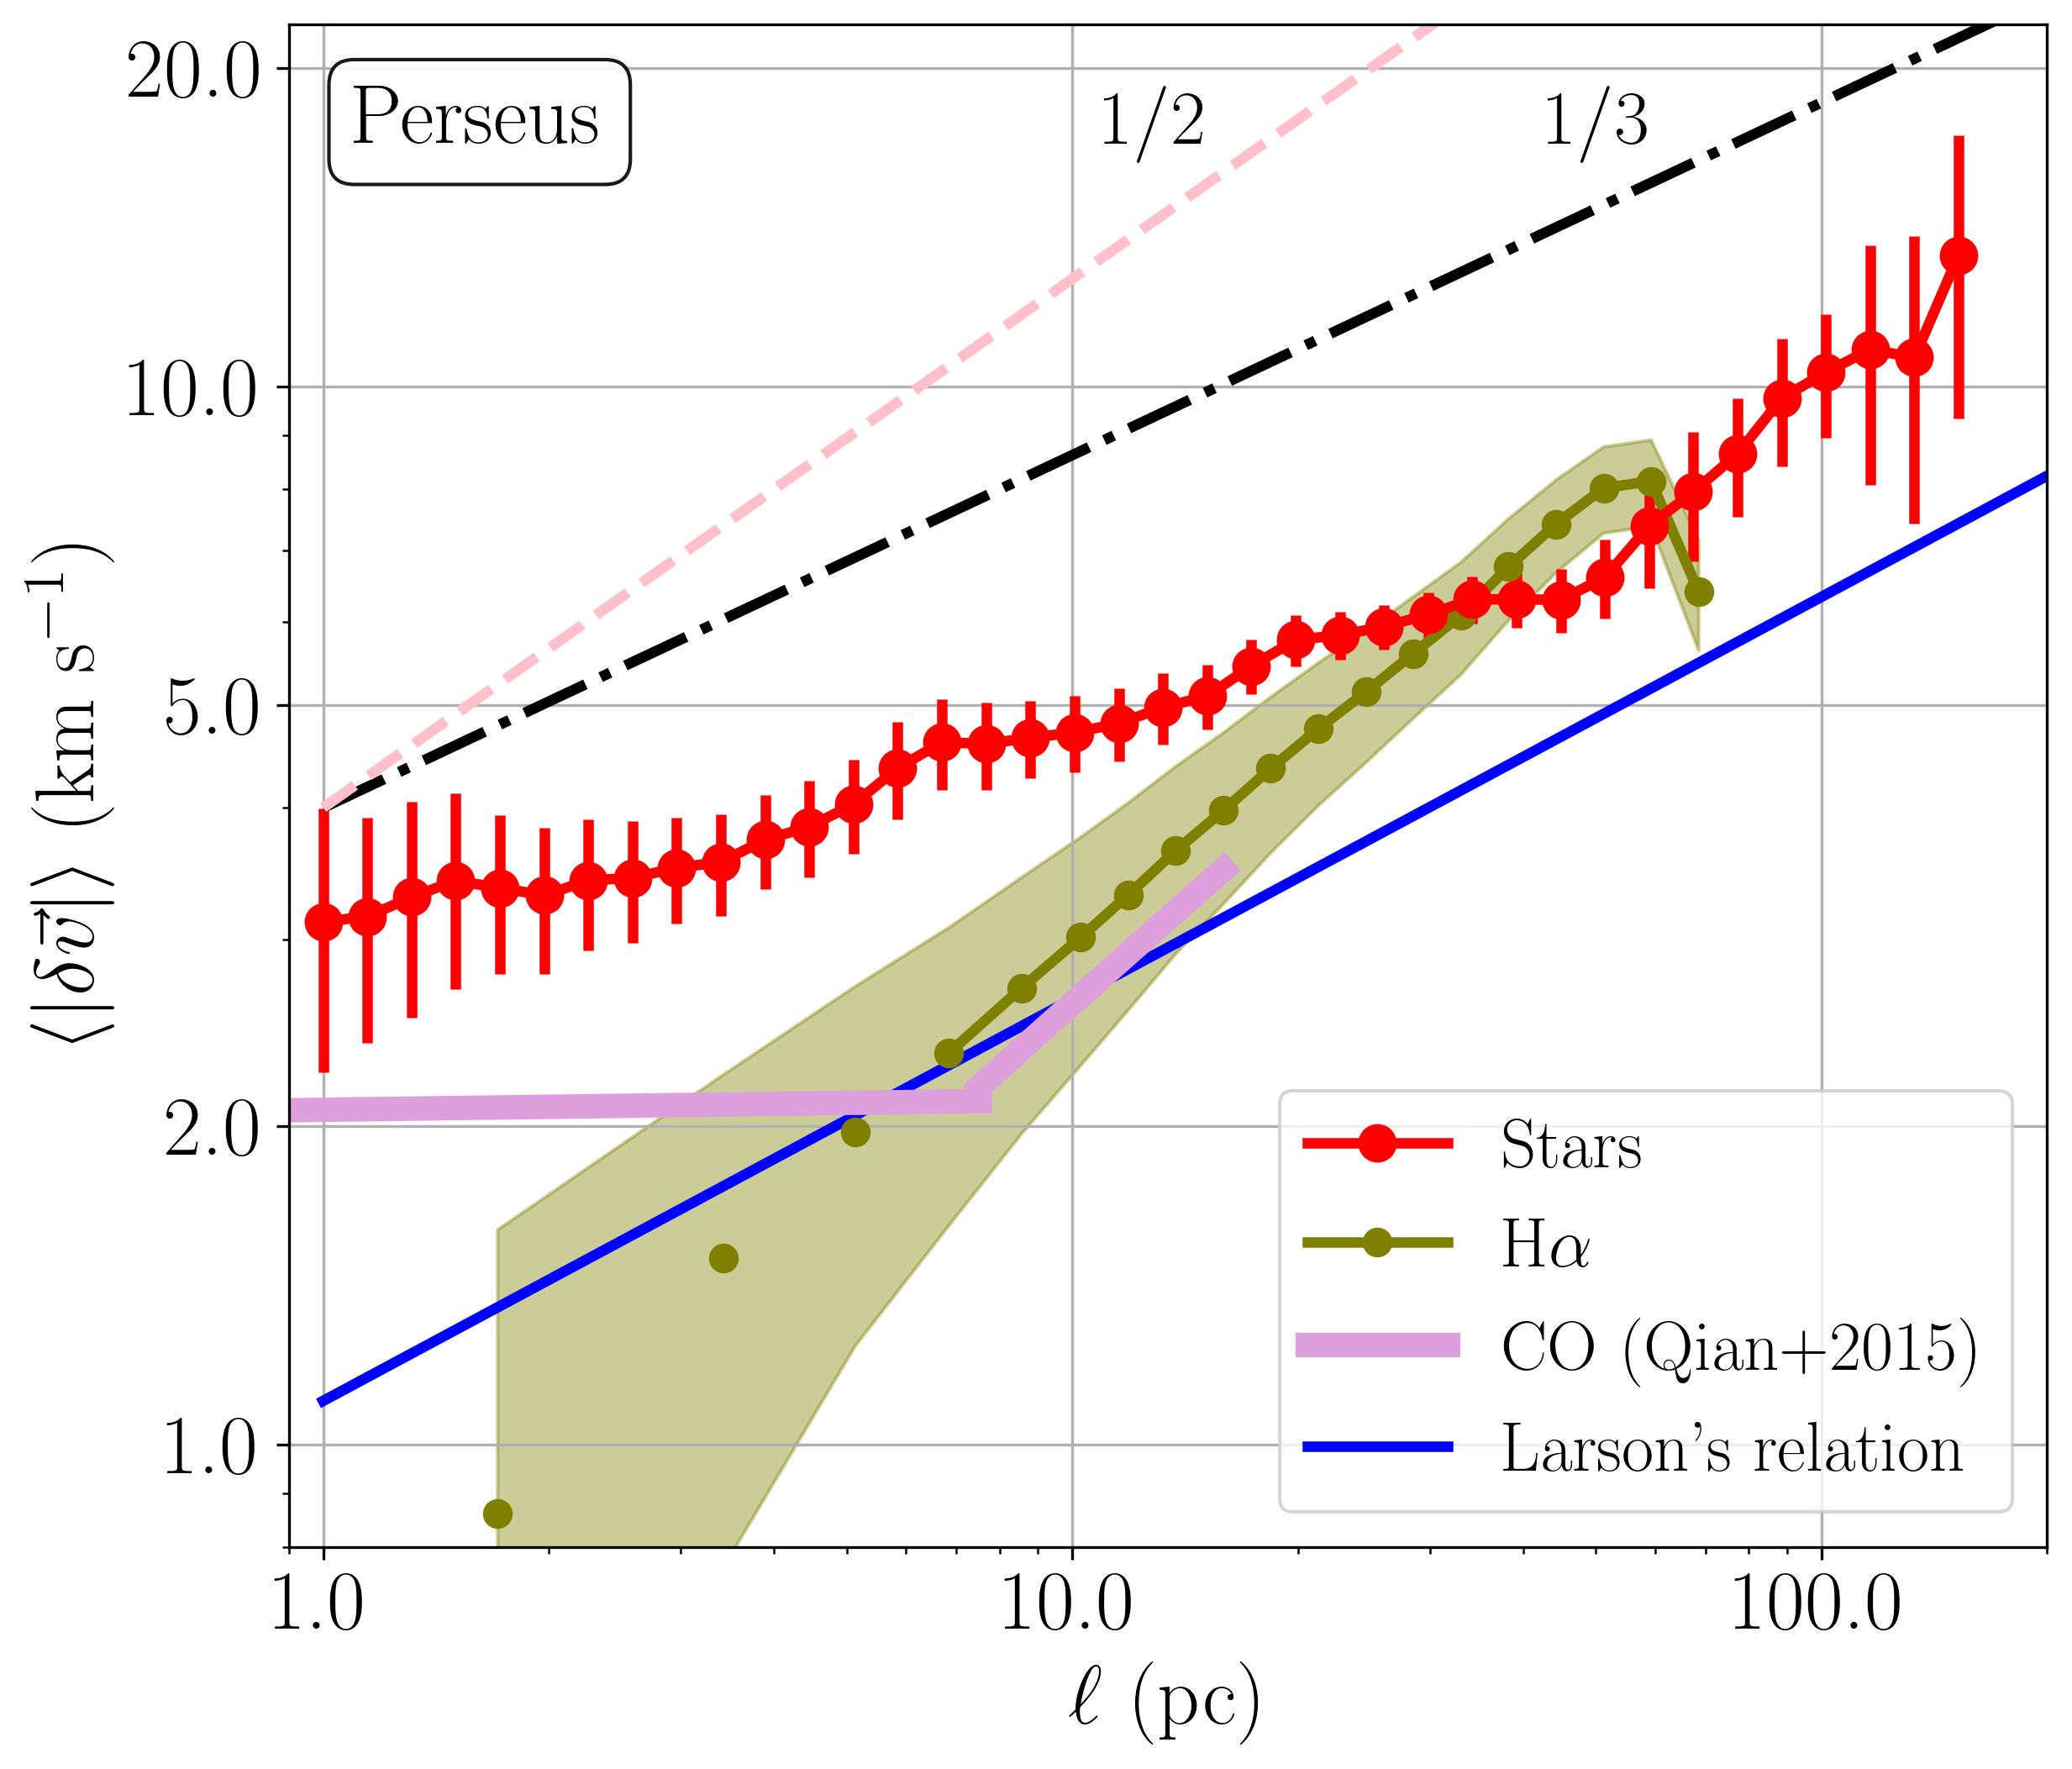
\includegraphics[width=0.48\linewidth]{Stars_img/Per_fill.png}
    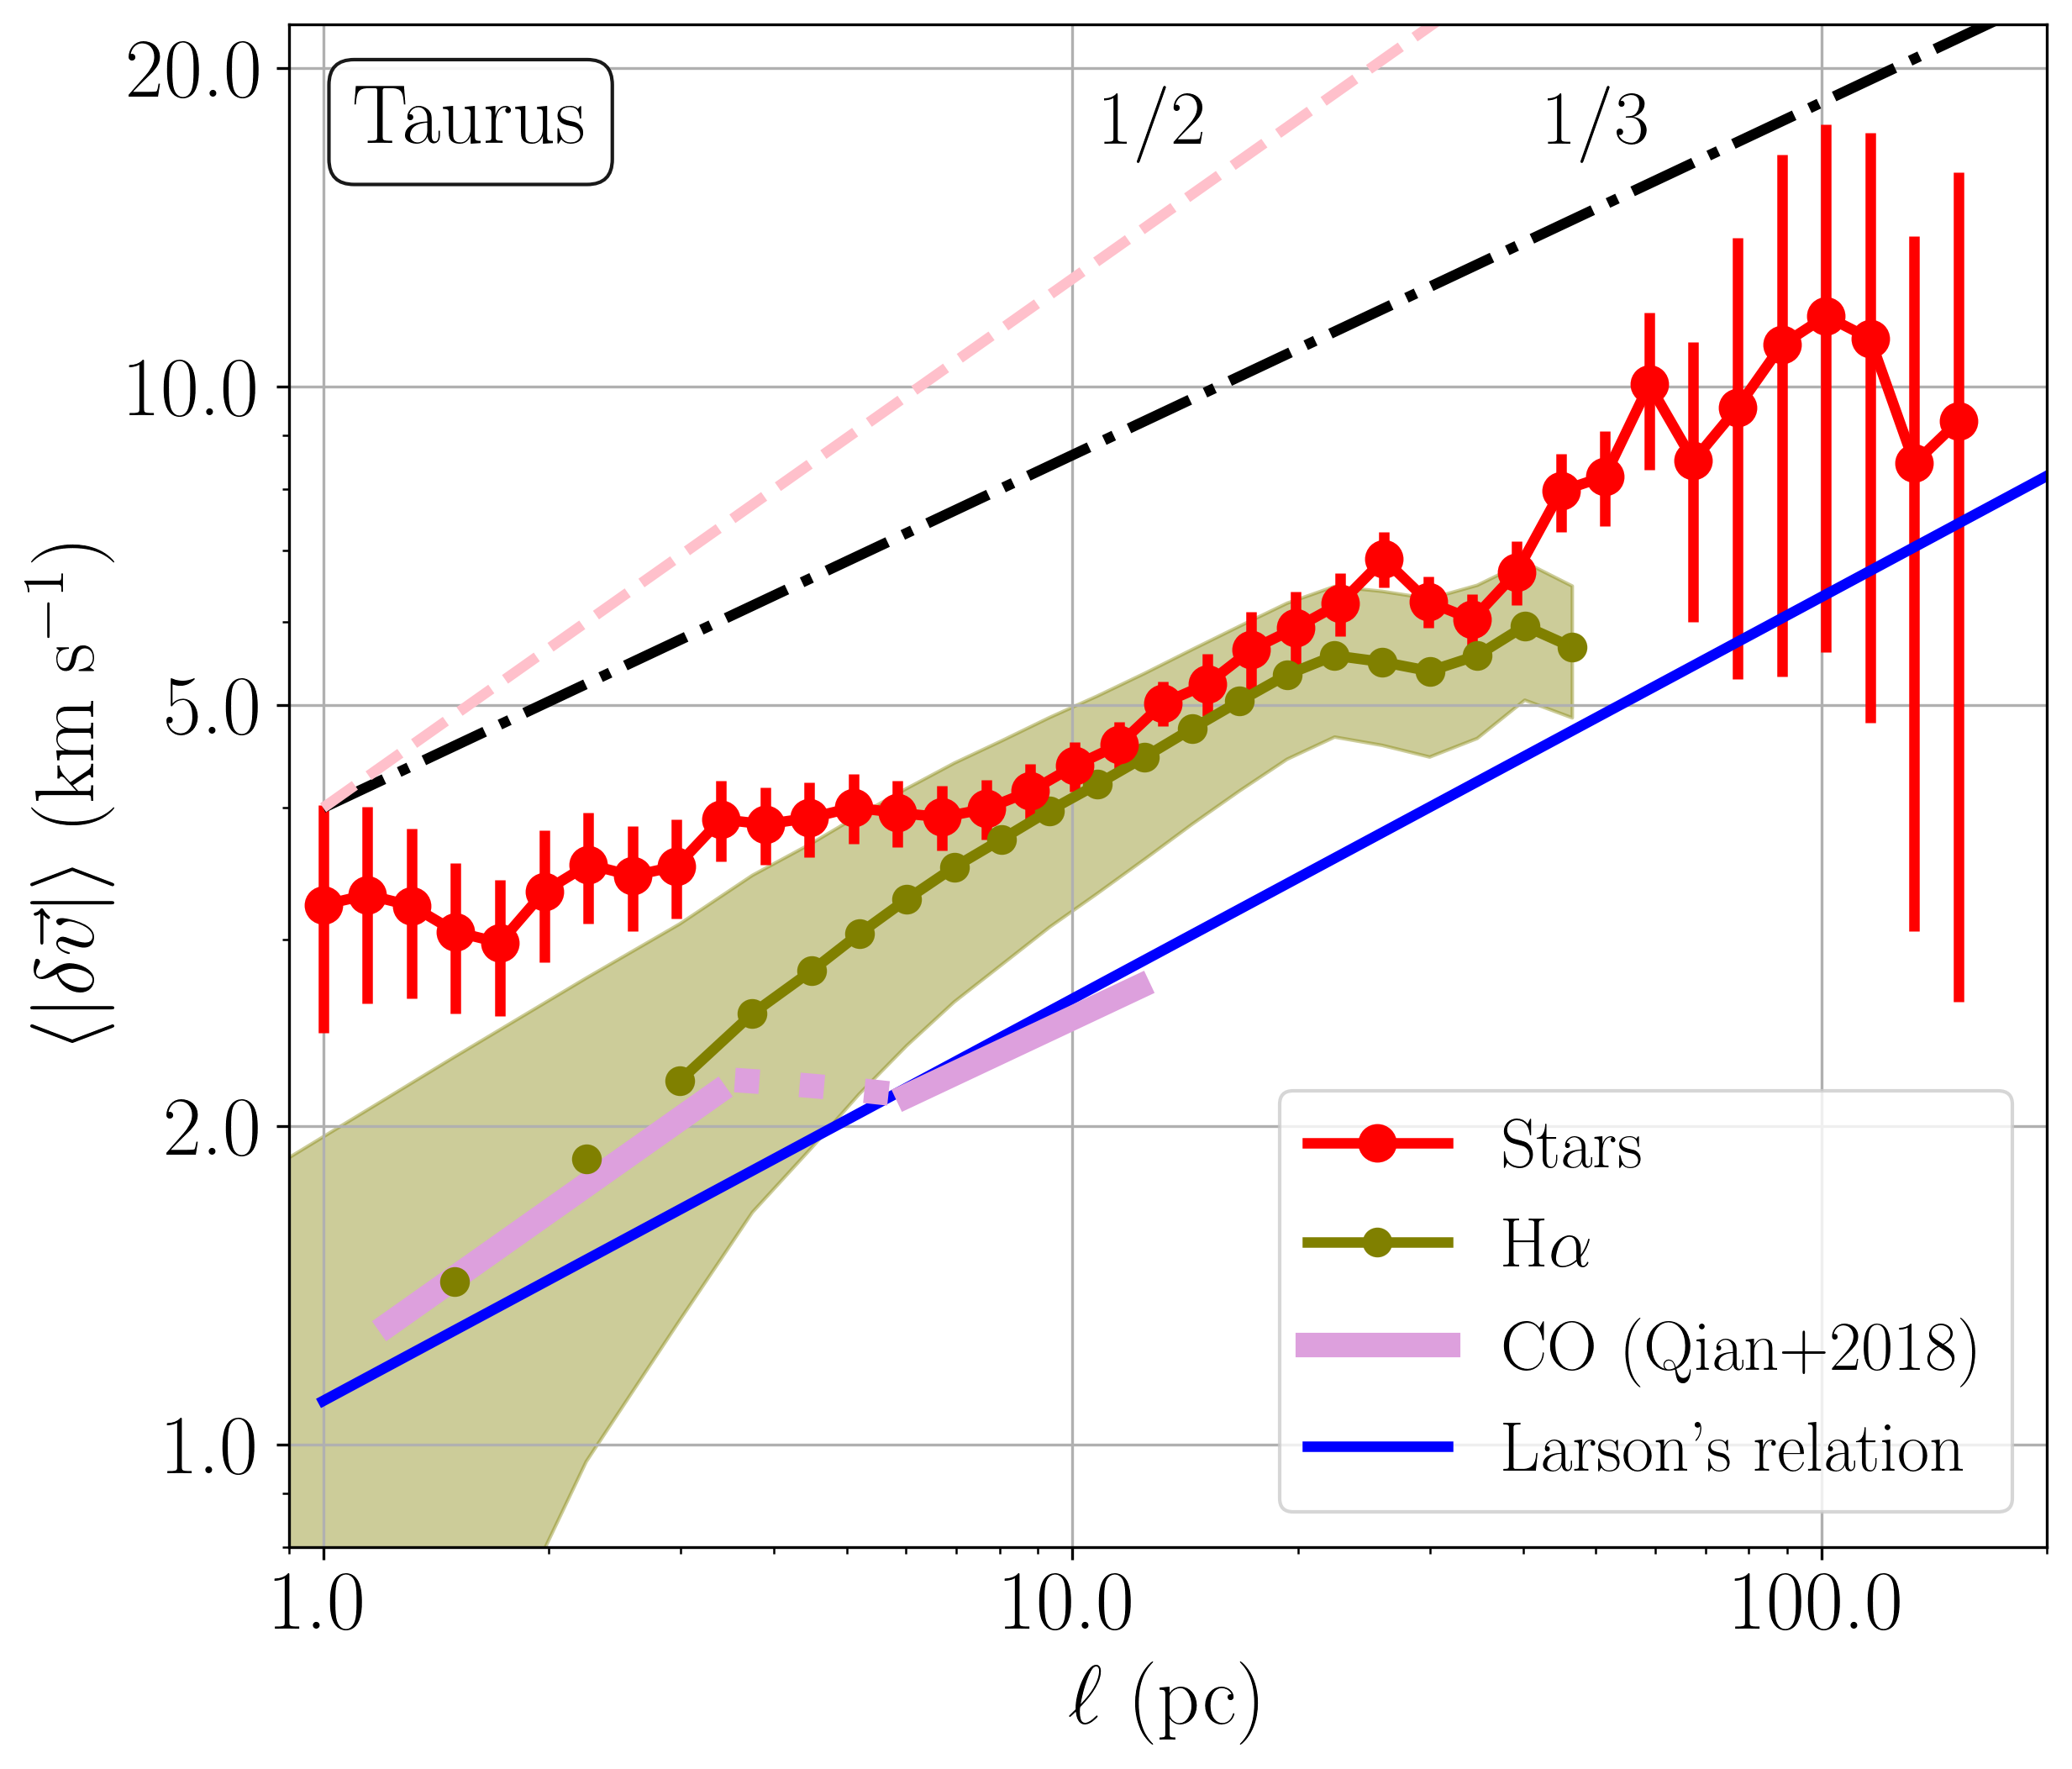
\includegraphics[width=0.48\linewidth]{Stars_img/Tau_fill.png}
    \caption{The first-order 3D VSF of stars (red) and H$\alpha$ (olive) for Orion, Ophiuchus, Perseus, and Taurus. The shaded region around the \halpha~VSF is its associated uncertainty. At small $\ell$, the dots showing the VSF traced by \halpha~are not connected to indicate the resolution limit of the WHAM survey ($\theta < 1$\textdegree). The slopes of the VSFs of stars and of \halpha~are specified in Table \ref{tab:slopes}. The VSF of \halpha~in Ophiuchus~can also be fitted with a broken power-law, with slope $0.58 \pm 0.24$ for $3~\mathrm{pc} < l < 9$~pc and slope $0.29 \pm 0.08$ for $9~\mathrm{pc} < l < 30$~pc. For comparison, we also include CO (violet) analysis from \citet{qian_new_2015,qian_studies_2018} for three of these regions.}
    \label{fig:stars_gas}
\end{figure*}

Figure \ref{fig:stars_gas} shows the VSFs of young stars as well as gas in each of the four regions: Orion, Ophiuchus, Perseus, and Taurus. The best-fit slopes of these VSFs are lists in Table~\ref{tab:slopes}.

\centerline{\textbf{Orion}}

The first-order VSF of Orion traced by stars has been studied in detail in Paper I. We only reiterate some of the main points here and address the differences caused by the addition of $\sim 1000$~stars compared with Paper I. 
Throughout the inertial range, the magnitude of $\langle |\delta \vec{v}| \rangle$~is higher than Larson's relation. At small scales ($1~\mathrm{pc} \lesssim \ell \lesssim 20$~pc), the number statistics is dominated by stars in the Orion Nebula Cluster (ONC), which flattens the VSF (see Section~\ref{sec:star_discussion} for more discussion on the small-scale flattening). 
At ranges from $20$~pc to $\sim 70$~pc, Orion D, which is a loose stellar association at the front of the Orion Complex along our line of sight, dominates the statistics, and it exhibits a power-law scaling, which indicates an imprint of turbulence from their natal molecular clouds. The VSF of Orion without considering the ONC would be steeper at small scales, which renders it more in-line with the VSF of other regions (see Figure \ref{fig:starsvsf}).
At $\sim 70$~pc, there is a bump in the structure function, and we proposed that this is an evidence supporting the existence of a SN explosion at the heart of Orion 6 Myr ago \citep{kounkel_supernovae_2020}.
Paper I used Gaia DR2 only. The newly added stars in this study from Gaia EDR3 have larger overall uncertainty in their parametric solutions. Therefore, the noise floor for Orion at small scales is boosted from $\sim 3$~km s$^{-1}$ to $\sim 5$~km s$^{-1}$. This slightly elevates the overall VSF compared to the values in Paper I.

\halpha~emission in Orion mainly comes from the Barnard's loop and the $\lambda$~Ori bubble (see Figure~\ref{fig:allsky}), which are thought to be created by SN explosions \citep{kounkel_supernovae_2020}. We see the effect of such energy injection in the VSF traced by \halpha. At $\ell \gtrsim 20$~pc, the amplitude of the \halpha~VSF is higher than the VSF of young stars. Over the whole dynamical range we probe here, the \halpha~VSF has a roughly constant slope of 1/2. 

The VSF traced by \halpha~shows a bump at $\ell \sim 150$~pc. This is indicative of a local energy injection, similar to those seen in the VSF traced by young stars. However, we caution that this scale is very close to the size of the \halpha~box, and the bump can also be an artifact \citep[see, e.g.,][]{mohapatra_velocity_2022}. We discuss this effect in more details in Section~\ref{sec:windowsize}. 
At very small scales ($\theta = 1^{\rm o}$, corresponding to $\ell \sim 7$~pc), our analysis is limited by the resolution of the WHAM survey \citep[][]{haffner_wisconsin_2003}. We discuss the effect of the resolution limit and other uncertainties related to \halpha~VSF in Section~\ref{sec:halpha_discussion}.

\centerline{\textbf{Ophiuchus}}

The young stars in Ophiuchus~has a VSF similar to that of the Orion Complex. At small $\ell$, the structure function is flatter than 1/3, and then steepens to $\sim$ 1/3 beyond 10 pc up to $\sim 25$~pc. The \halpha~VSF in Ophiuchus has slope close to 1/3 and a higher amplitude than the VSF of the stars. Both VSFs show clear bumps at $\sim 25$~pc, which we interpret as evidence of local energy injection.

In Orion, such an energy injection is associated with a past SN explosion as we discuss in detail in Paper I. If the energy injection in Ophiuchus is also caused by a SN, we estimate that the event took place around $25\,\mathrm{pc} / v_{\rm region} \sim 2.5$~Myr ago, where we use the characteristic \halpha~velocity $v_{\rm region}\sim 10$~km s$^{-1}$. Such an estimate is broadly consistent with observations of runaway stars which trace back to a SN explosion in the region $\sim 2$~Myr ago \citep[][]{neuhauser_nearby_2020}. 

We note that the scale of the bump is close to the size of the region containing the young stars in our analysis. Therefore, it is technically possible that the bump in the VSF of young stars is only an artifact caused by the limited sample size. In Section~\ref{sec:Upper_Sco}, we analyze the entire Upper Sco region. We find that as long as we apply our analysis to young stars ($< 2$~Myr), the results are consistent, while the VSFs of older stars do not show this feature. In addition, the SN scenario is also supported by the bump in the \halpha~VSF.

The cold and dense molecular cores, where stars are born out of, emits CO. \citet{qian_new_2015,qian_studies_2018} applied the core-velocity-dispersion \citep[CVD;][]{qian_13co_2012}~method to analyze turbulence in star-forming regions. We translate their best-fit CVD to a VSF of CO by $\mathrm{VSF} = \sqrt{\frac{2}{\pi}}~\mathrm{CVD}$. 

In Ophiuchus, the amplitude of CO VSF (pink solid lines in Figure \ref{fig:stars_gas}) is much lower than the VSF of young stars and \halpha. It is possible that the recent energy injection has affected the warm phase of the ISM more than the cold phase (see discussion in Section~\ref{sec:nature_ISM}). It is also possible that the low amplitude is due to spatial variation of ISM turbulence (see discussion in Section~\ref{sec:windowsize}). \citet[][]{qian_new_2015} only examined the smaller scale velocity structures ($\ell \lesssim 10$~pc), where there is no reliable component that we can compare against (due to relaxation of stars and resolution limit of \halpha).

\centerline{\textbf{Perseus}}

At length scales below 10 pc, the VSF of young stars in Perseus is very similar to that of Ophiuchus~(see Figure \ref{fig:starsvsf}). Since we include two clusters in our analysis of Perseus: NGC 1333 and IC 348, the VSF is flattened from internal dynamical relaxation. The existence of subgroups and sub-clusters are likely the cause of the small wiggles in the VSF\@. At larger scales, the VSF is generally consistent with Larson's relation.

The VSF traced by \halpha~here has an amplitude similar to the VSF traced by young stars but a steeper slope ($\sim$ 1/2). VSF traced by CO matches the \halpha~ VSF at $\ell > 6$~pc, but flattens on smaller scales due to projection effects for thick clouds \citep[][]{qian_new_2015, xu_projected_2020}.

\centerline{\textbf{Taurus}}

Taurus is overall very similar to Perseus. The VSFs of young stars, \halpha~and CO generally agree with each other, as well as Larson's relation.

There is no prominent bump detected in the VSF in both Perseus and Taurus, which is consistent with the findings of \citet[][]{krolikowski_gaia_2021}~that there has been no SN activities in the last 5 Myr in these regions. However, there are wiggles scattered throughout the length scales, likely because Taurus contains several small dense groups that are primarily homogeneously distributed throughout the region.

\begin{table}
    \centering
    \caption{Slopes of the VSFs}
    \label{tab:slopes}
    \begin{tabular}{ccccc}
        \toprule
        Region    &
        Slope of       &
        Fitting        &
        Slope of           &
        Fitting            \\
                  &
        stars VSF      &
        range (pc)     &
        \halpha~VSF        &
        range (pc)         \\
        \midrule
        Orion     & $0.25 \pm 0.01$ & $12$--$75$ & $0.55 \pm 0.02$ & $9$--$150$ \\
        Ophiuchus & $0.34 \pm 0.03$ & $7$--$28$  & $0.36 \pm 0.03$ & $3$--$30$  \\
        Perseus   & $0.22 \pm 0.03$ & $5$--$80$  & $0.61 \pm 0.08$ & $7$--$55$  \\
        Taurus    & $0.34 \pm 0.03$ & $7$--$70$  & $0.42 \pm 0.12$ & $3$--$25$  \\
        \bottomrule
    \end{tabular}
    \parbox{\linewidth}{\footnotesize \textit{Note.} Inside the fitting ranges, the VSFs are fitted with an equation: \vsf~$= A \cdot \ell^{B}$, where $B$~is the slope. The uncertainties reported with each slope is obtained from the covariance matrix, taking into account the uncertainties in \vsf~shown in Figure~\ref{fig:stars_gas}. We choose the fitting ranges such that the uncertainties are low and there is a consistent trend in the slope of the VSF.}
\end{table}

\subsection{Discussion} \label{sec:multi-region-discussion}

\subsubsection{Uncertainties and biases in turbulence traced by young stars} \label{sec:star_discussion}

We discussed various biases and uncertainties associated with measuring turbulence from stars in Paper I, including dynamical relaxation, binary contamination, and drifting. In this section, we reiterate the main points and discuss additional mechanisms that can affect the shape of the VSF.

Stellar interactions can cause dynamical relaxation, which erases the memory of turbulence and flattens the VSF\@. Similar to Orion's loose groups discussed in Paper I, the relaxation times of Ophiuchus, Perseus, and Taurus are estimated to be tens of Myrs, much longer than their age \citep[for a detailed discussion of the age of each region, see][]{wilking_star_2008,krolikowski_gaia_2021,pavlidou_substructure_2021}. Thus dynamical relaxation has not affected the overall shape of the VSF for the three regions. However, there are some small, compact star clusters in these regions, which can contribute to the flattening at small scales ($\ell \lesssim 10$~pc, see Figure \ref{fig:starsvsf}).

Another source of uncertainty originates from the drifting of stars along their natural trajectories over time. Stars born with high velocity differences drift apart at faster rates than stars born with low velocity differences, which steepens the VSF roughly over the crossing time ($t_{\rm cross}$) of the cloud. Similar to the star groups in Orion that we discussed in Paper I, $t_{cross}$ of Ophiuchus, Perseus, and Taurus are all larger than their current age, and thus this effect is unlikely to have significantly altered the shape of the structure functions.

Low-velocity binary systems and contamination from field stars can act like noise in our analysis, which also tends to flatten the VSF as is discussed in Paper I.

Additionally, other stellar feedback processes such as winds, jets, and radiation can also inject energy on small scales \citep[e.g.,][]{gritschneder_driving_2009, offner_impact_2015, li_disruption_2019, rosen_blowing_2021, grudic_dynamics_2022}. This can contribute to the flattening of the VSFs at small scales, provided that these stars are massive ($> 8~M_{\odot}$) and are within $\sim 1$~pc of each other \citep[][]{rosen_blowing_2021}. 

\citet{stutz_slingshot_2016} quantified an ejection mechanism through which protostars decouple from the molecular gas. They found that the undulation of star-forming filaments in Orion A ``slingshots" protostars out of the filament at $\sim 2.5$~km~s$^{-1}$, which is also at the level where the VSF flattens in Ophiuchus, Perseus, and Taurus. 

All sources of uncertainties listed above can contribute to the flattening of the VSF at small scales ($\ell \lesssim 10$~pc). Therefore, we only consider young stars to be reliable tracers of ISM turbulence above $\sim 10$~pc.

The completeness of the stellar sample may also affect the VSFs. In Orion, the current stellar population with 6D measurements are estimated to cover about 25\% of the total number of young stars in the region \citep[][]{kounkel_untangling_2019}. In the other regions, the coverage of our sample is $\sim 20\text{--}30\%$ \citep[see,][]{luhman_census_2016,briceno-morales_substructure_2022,krolikowski_gaia_2021}.

If more young stars are observed in the future with levels of uncertainties similar to the existing data, we expect better statistics. Therefore, having a more complete sample of young stars in these regions can further strengthen the conclusion of our analysis. However, having a more complete sample of the young stellar population does not necessarily translate to better accuracy of the VSF analysis. In Orion, we obtained an additional $\sim 1000$~stars going from Gaia DR2 (Paper I) to Gaia EDR3 (this work). However, these new stars have higher astrometric uncertainties compared to the ones previously identified in Gaia DR2, and thus the noise level of the VSF is elevated, and the slope of the VSF flattens compared to what we found in Paper I.

\subsubsection{ISM Turbulence traced by \texorpdfstring{\halpha}{H-alpha}}
\label{sec:halpha_discussion}

In Figure \ref{fig:starsvsf} and Figure \ref{fig:stars_gas}, we find that while the VSFs of stars are broadly consistent across the regions, the VSFs of \halpha~are more diverse.

In regions with recent supernova explosions (Orion and Ophiuchus), the VSF of \halpha~gas has a higher amplitude than that of stars. Whereas in Perseus and Taurus, the \halpha~flux is lower (Figure~\ref{fig:allsky}) and the \halpha~VSF is more in line with the VSFs of stars and CO.

\begin{figure}
    \centering
    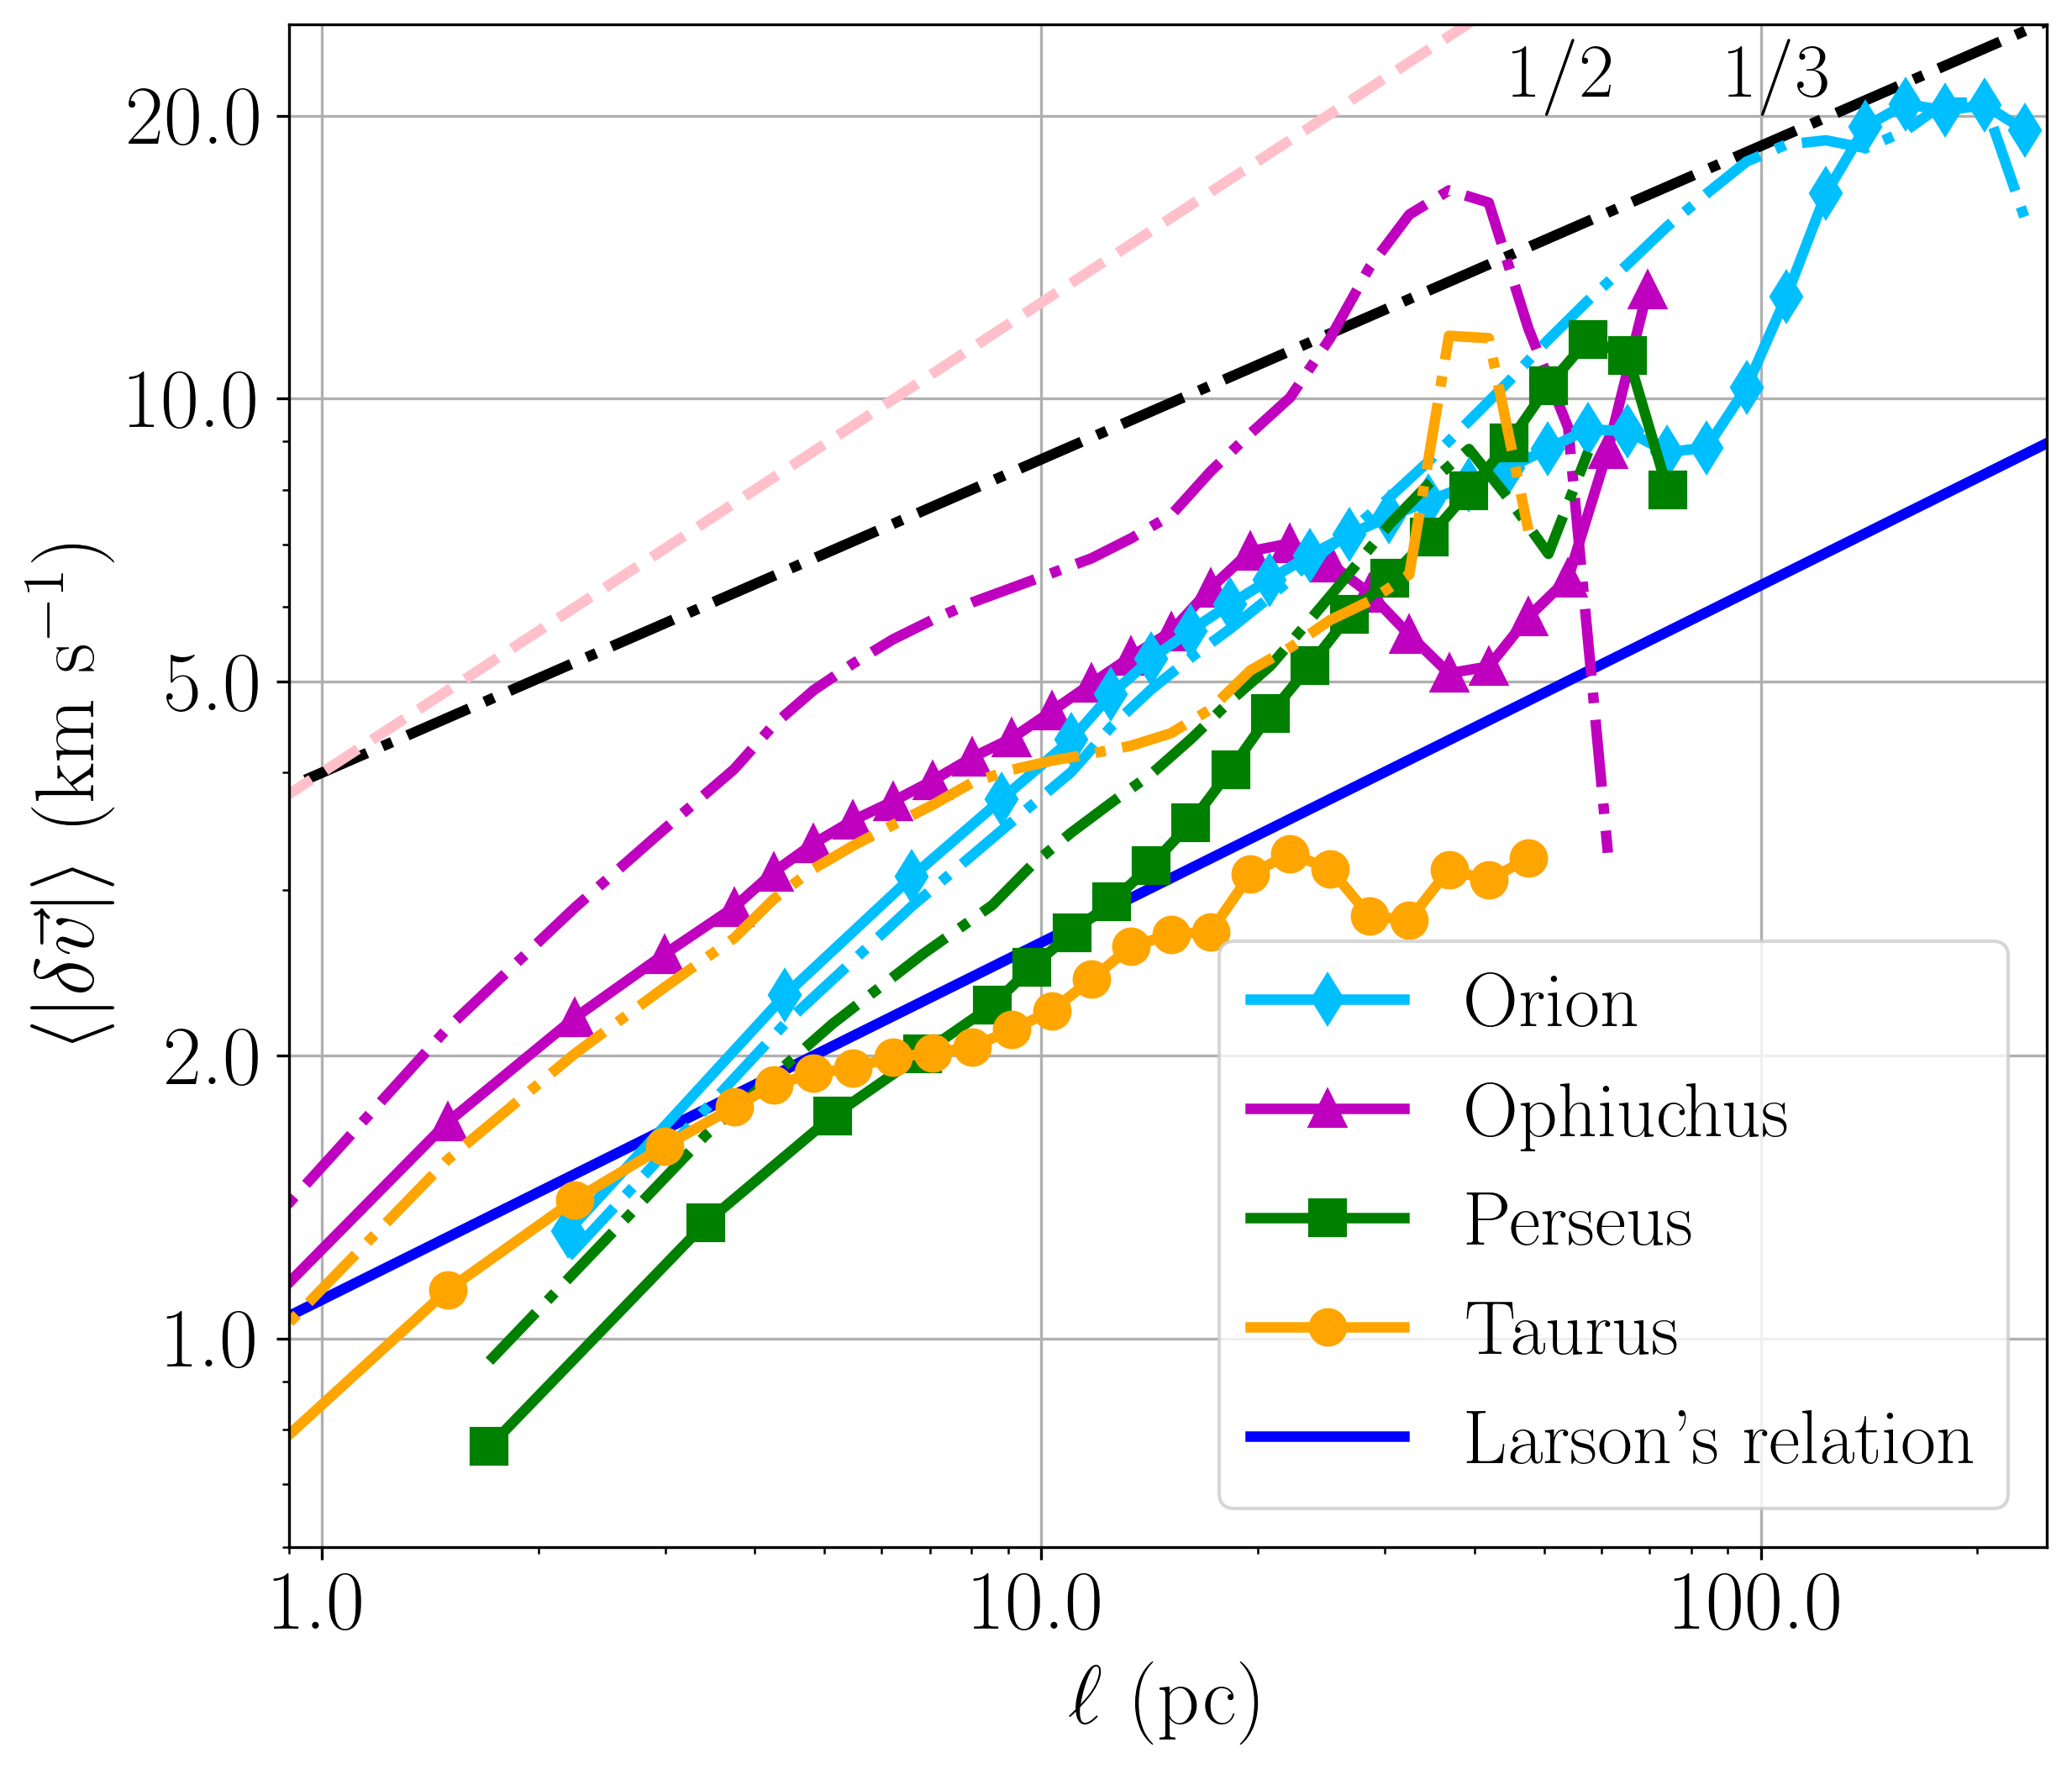
\includegraphics[width=\linewidth]{Stars_img/emission_test.png}
    \caption{VSF of four regions traced by \halpha. Solid lines denote the VSF computed for pixels with low emission, and dotted-dashed lines denote the VSF computed for pixels with high emission.}
    \label{fig:emission}
\end{figure}

Within each individual region, we divide the pixels in half based on the \halpha~brightness---the high-emission half with all the pixels brighter than the median and the low-emission half with all the pixels dimmer than the median. Figure \ref{fig:emission}~shows the VSFs of high-emission \halpha~(dotted-dashed line) and low-emission \halpha~(solid line) within each region. In general, the VSF of high-emission \halpha~has a higher amplitude compared to that of the low-emission \halpha\ component.

One possible explanation for this is that bright \halpha~comes from photo-ionization by young massive stars \citep{tacchella_hensuremathalpha_2022}. Therefore, it traces the most intense stellar feedback regions and shows a higher VSF amplitude. Whereas the low-emission \halpha~comes primarily from collisional ionization. Note that Orion has its high- and low-emission \halpha~ VSFs essentially overlapping for the most part. This is likely because star formation in Orion is the most intense among all the regions studied here \citep[see Table 2 of][]{lada_star_2010}, and thus most of the \halpha~is photo-ionized by massive stars.

There are many uncertainties and potential biases associated with the \halpha~analysis. One source of uncertainty comes from the resolution limit. Although the WHAM data cubes is sampled every 0.25\textdegree, the reported spatial resolution of the survey is 1\textdegree~\citep[][]{haffner_wisconsin_2003}. At separations $\theta \leq 1$\textdegree~(or $\ell_{\rm proj} \leq d \cdot 1$\textdegree), we treat the VSF traced by \halpha~as unresolved (represented by the unconnected dots in Figure \ref{fig:stars_gas}). We note that resolution limit might not significantly alter the overall VSF, as suggested by \citet{li_direct_2020}. Future studies with mock simulated \halpha~observations may help properly evaluate the effects of the resolution limit of the dataset. 

There are also uncertainties with the distance to the \halpha~gas. The bright \halpha~emissions in Orion and Ophiuchus~are likely associated with the star forming regions. However, since Perseus and Taurus do not emit intense \halpha~(see top right panel of Figure \ref{fig:allsky}), it is uncertain whether the centroid velocities found in these two regions are at the exact same distance as the stars.

Another bias can come from the projection effects. When analyzing the VSF of \halpha, we assume that all the gas is located at the same distance, effectively treating it as a 2D structure. This can flatten the VSF for thick clouds, as is discussed in detail in \citet{qian_new_2015, xu_projected_2020, mohapatra_velocity_2022}. All the \halpha~VSFs in our analysis are either as steep as 1/3 or steeper. This suggests that either most of the \halpha~comes from a thin sheet of gas, or the true VSF has an even steeper slope.

Another potential bias related to projection is that we are trying to infer 3D turbulence using projected 2D information. This can introduce uncertainties as the ISM is magnetized. In the presence of magnetic fields, turbulence is no longer isotropic \citep{seifried_impact_2015, hu_anisotropic_2021}. We find that our results are not sensitive to the rotation model (see detailed discussions in Section~\ref{sec:rotation}). 

\subsubsection{The Complex Nature of ISM Turbulence}
\label{sec:nature_ISM}

The ISM is multiphase in nature. The kinematic coupling between these phases is not well understood \citep[for a review of the multiphase ISM model, see][]{cox_three-phase_2005}. More specifically, it is suggested that each phase possesses varying levels of turbulence, where ionized gas has been observed to have higher velocity dispersion than molecular gas in both high- and low-redshift galaxies \citep[][]{girard_systematic_2021,ejdetjarn_giant_2022}. In our study, we observe a similar trend comparing the VSF of \halpha~and other tracers of turbulence.

In Orion and Ophiuchus, there is a large deviation between the level of turbulence seen by different tracers. The VSFs traced by \halpha~show the largest amplitude at large scales, followed by the VSFs traced by stars, and finally by CO\@. One possible explanation is the difference in the transport of energy and momentum from SNe into different phases in these regions, as mentioned in Section \ref{subset:eachregion_result}. In an inhomogeneous medium such as the Milky Way ISM, SNe carry shocked matter radially outward following the path of least resistance. As a consequence, the cool dense phase traced by CO receives less energy injection than the warm diffuse phase traced by \halpha, resulting in lower levels of turbulence in the corresponding VSF\@. Such behavior is also seen in hydrodynamical simulations of single SN remnants \citep[e.g.,][]{martizzi_supernova_2015,li_supernova_2015}.

In Perseus and Taurus, the VSFs traced by \halpha~and CO show a good agreement in both the amplitudes and slopes in these regions, except for the range $\ell \lesssim 7$~pc in Perseus, which suffers from projection effect due to the thickness of the cloud \citep[see Section 4.2 of][for a detailed discussion]{qian_new_2015}. At larger $\ell$, the VSF traced by \halpha~and stars also closely follow each other. Such trend is consistent with the evolutionary history of these regions with no clear imprint of recent SN explosions. Without this important local driver of turbulence, different phases of gas are well-coupled, and the young stars formed out of these molecular clouds also largely retain the same memory of turbulence. 

At length scales beyond the bumps caused by SN energy injection, we recognize a common upward trend in the VSFs of stars. In all four regions, the VSFs at the largest $\ell$~maintain a positive slope with no apparent driving scale. At these length scales, the ISM turbulence is driven primarily by galactic shear \citep[see, e.g.,][]{gammie_velocity_1991} and accretion flows onto the galaxy \citep[][]{forbes_gas_2023}.

The difference of \halpha~VSFs in different regions show that ISM turbulence can be unevenly distributed spatially as a result of local drivers. Turbulence can also be unevenly distributed between different phases of the ISM (e.g., Orion and Ophiuchus). Section~\ref{sec:halpha_discussion} and Figure~\ref{fig:emission} further demonstrate that even with the same gas tracer \halpha, the level of turbulence can vary depending on its brightness. In addition, we note that local energy injection from supernova explosions is also intermittent temporally. Using the \halpha~VSF in Ophiuchus, we estimate the eddy turnover time at the driving scale to be:
\begin{equation}
\frac{\ell}{v}\sim \frac{20\text{--}30\,\mathrm{pc}}{5\,\mathrm{km\,s^{-1}}}\sim 4\text{--}6\,\mathrm{Myr}.
\end{equation}
The \halpha~VSF in Orion gives a similar estimate. Typically, it takes a few eddy turnover times to establish a steady-state turbulent flow. On the other hand, given the size of these regions, the average time interval between supernovae is on the order of a few Myr \citep{narayan_pulsar_1990, li_supernova_2015}. Each event also injects energy as a pulse with a very short duration. Therefore, both the ``on'' and ``off'' states of the driver are short compared with the timescale required to achieve a steady state. Thus ISM turbulence in molecular complexes is often not in a steady state.


\subsection{Conclusions} \label{sec:conclusions}

In this work, we analyze the kinematics of young stars and gas in four nearby star-forming regions: Orion, Ophiuchus, Perseus, and Taurus. For each region, we compute the first-order VSF of young stars and \halpha~gas, and compare the results against each other, as well as analysis of CO molecular cores from the literature.

We find that the VSFs traced by young stars in all four regions exhibit similar properties largely in agreement with Larson's relation and reveal a universal scaling of turbulence in the ISM\@. This also confirms our previous finding in \citet[][]{ha_measuring_2021} that young stars retain the memory of turbulence in their natal molecular clouds, and thus can be used to measure the turbulent kinematics of molecular clouds.

The VSFs of \halpha~are more diverse, likely as a result of local energy injection. In regions with recent SN activities such as Orion and Ophiuchus, the VSFs of \halpha~are higher in amplitude compared to those without. The \halpha~VSFs are also higher than the VSFs of stars and CO in these regions, while regions without recent SN explosions (Perseus and Taurus) show well-coupled turbulence between different phases. Within each individual region, the high-emission \halpha~tends to show higher VSFs than the low-emission \halpha.

Our findings support a complex picture of the Milky Way ISM, where turbulence can be driven at different scales and inject energy unevenly into different phases. Future observations with more tracers of turbulence and on more star forming regions will help us better understand the diversity and complexity of ISM turbulence. In addition, high-resolution numerical studies can help further our understanding of the coupling between different phases and relevant timescales.


\subsection{Supplemental Material}

\subsubsection{Selection of the \texorpdfstring{\rophi}{rho Oph}~dark cloud within the Upper Sco region}
\label{sec:Upper_Sco}

\begin{figure}
    \centering
    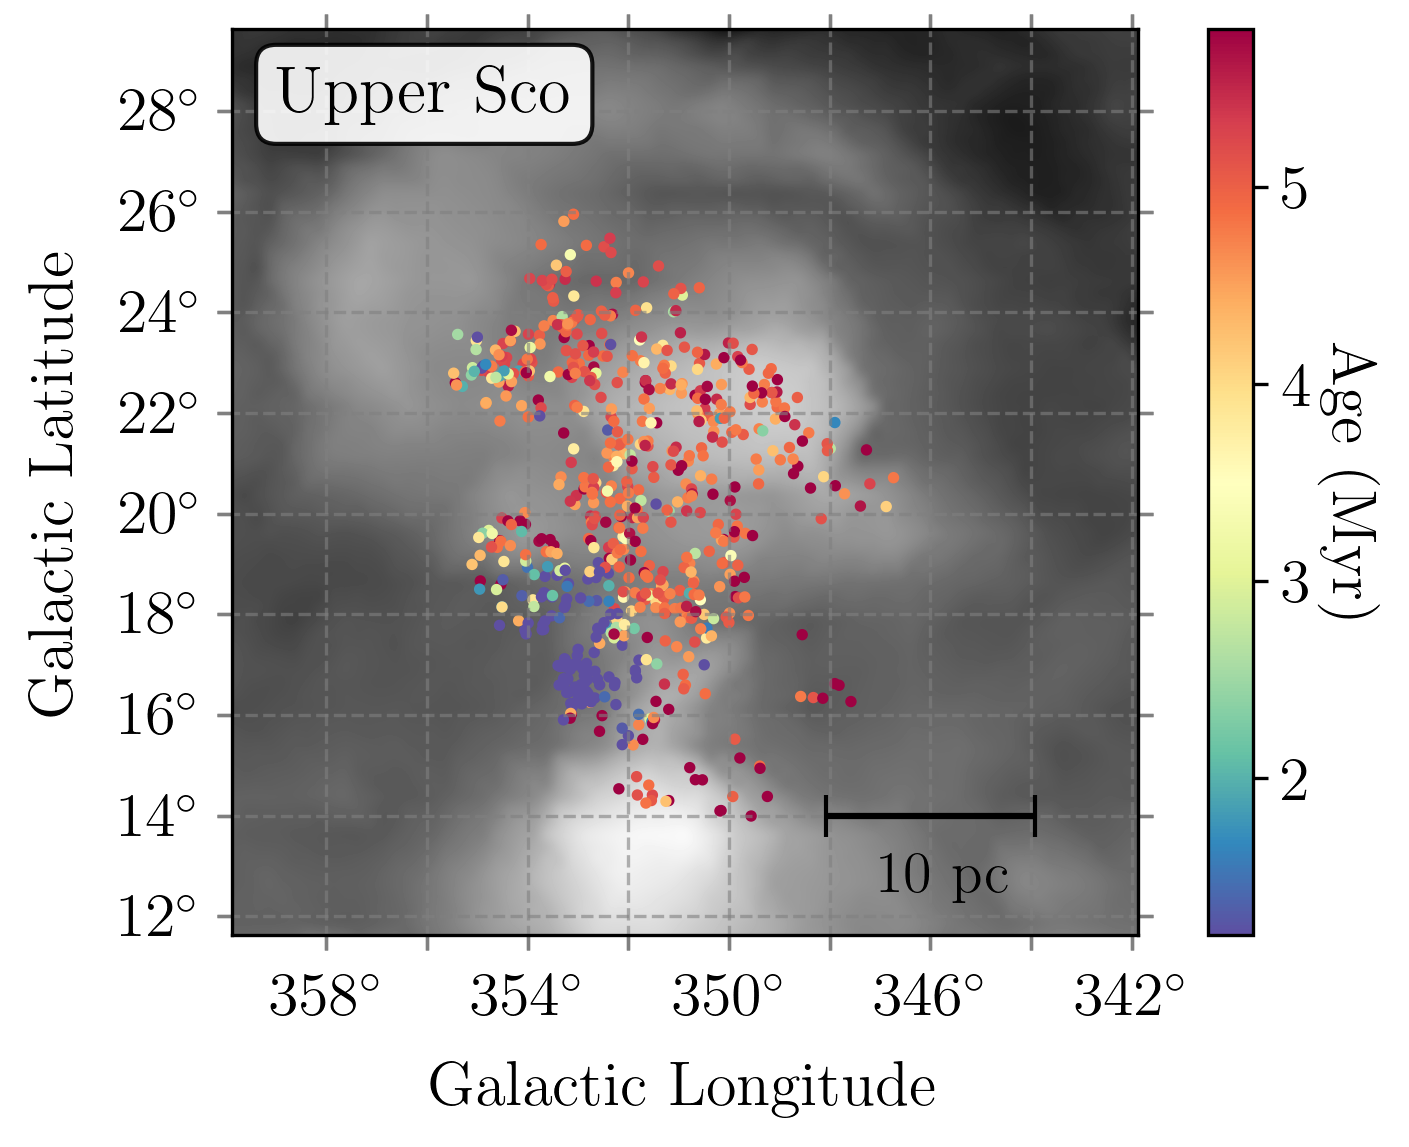
\includegraphics[width=0.7\columnwidth]{Stars_img/UpperSco_age.png}
    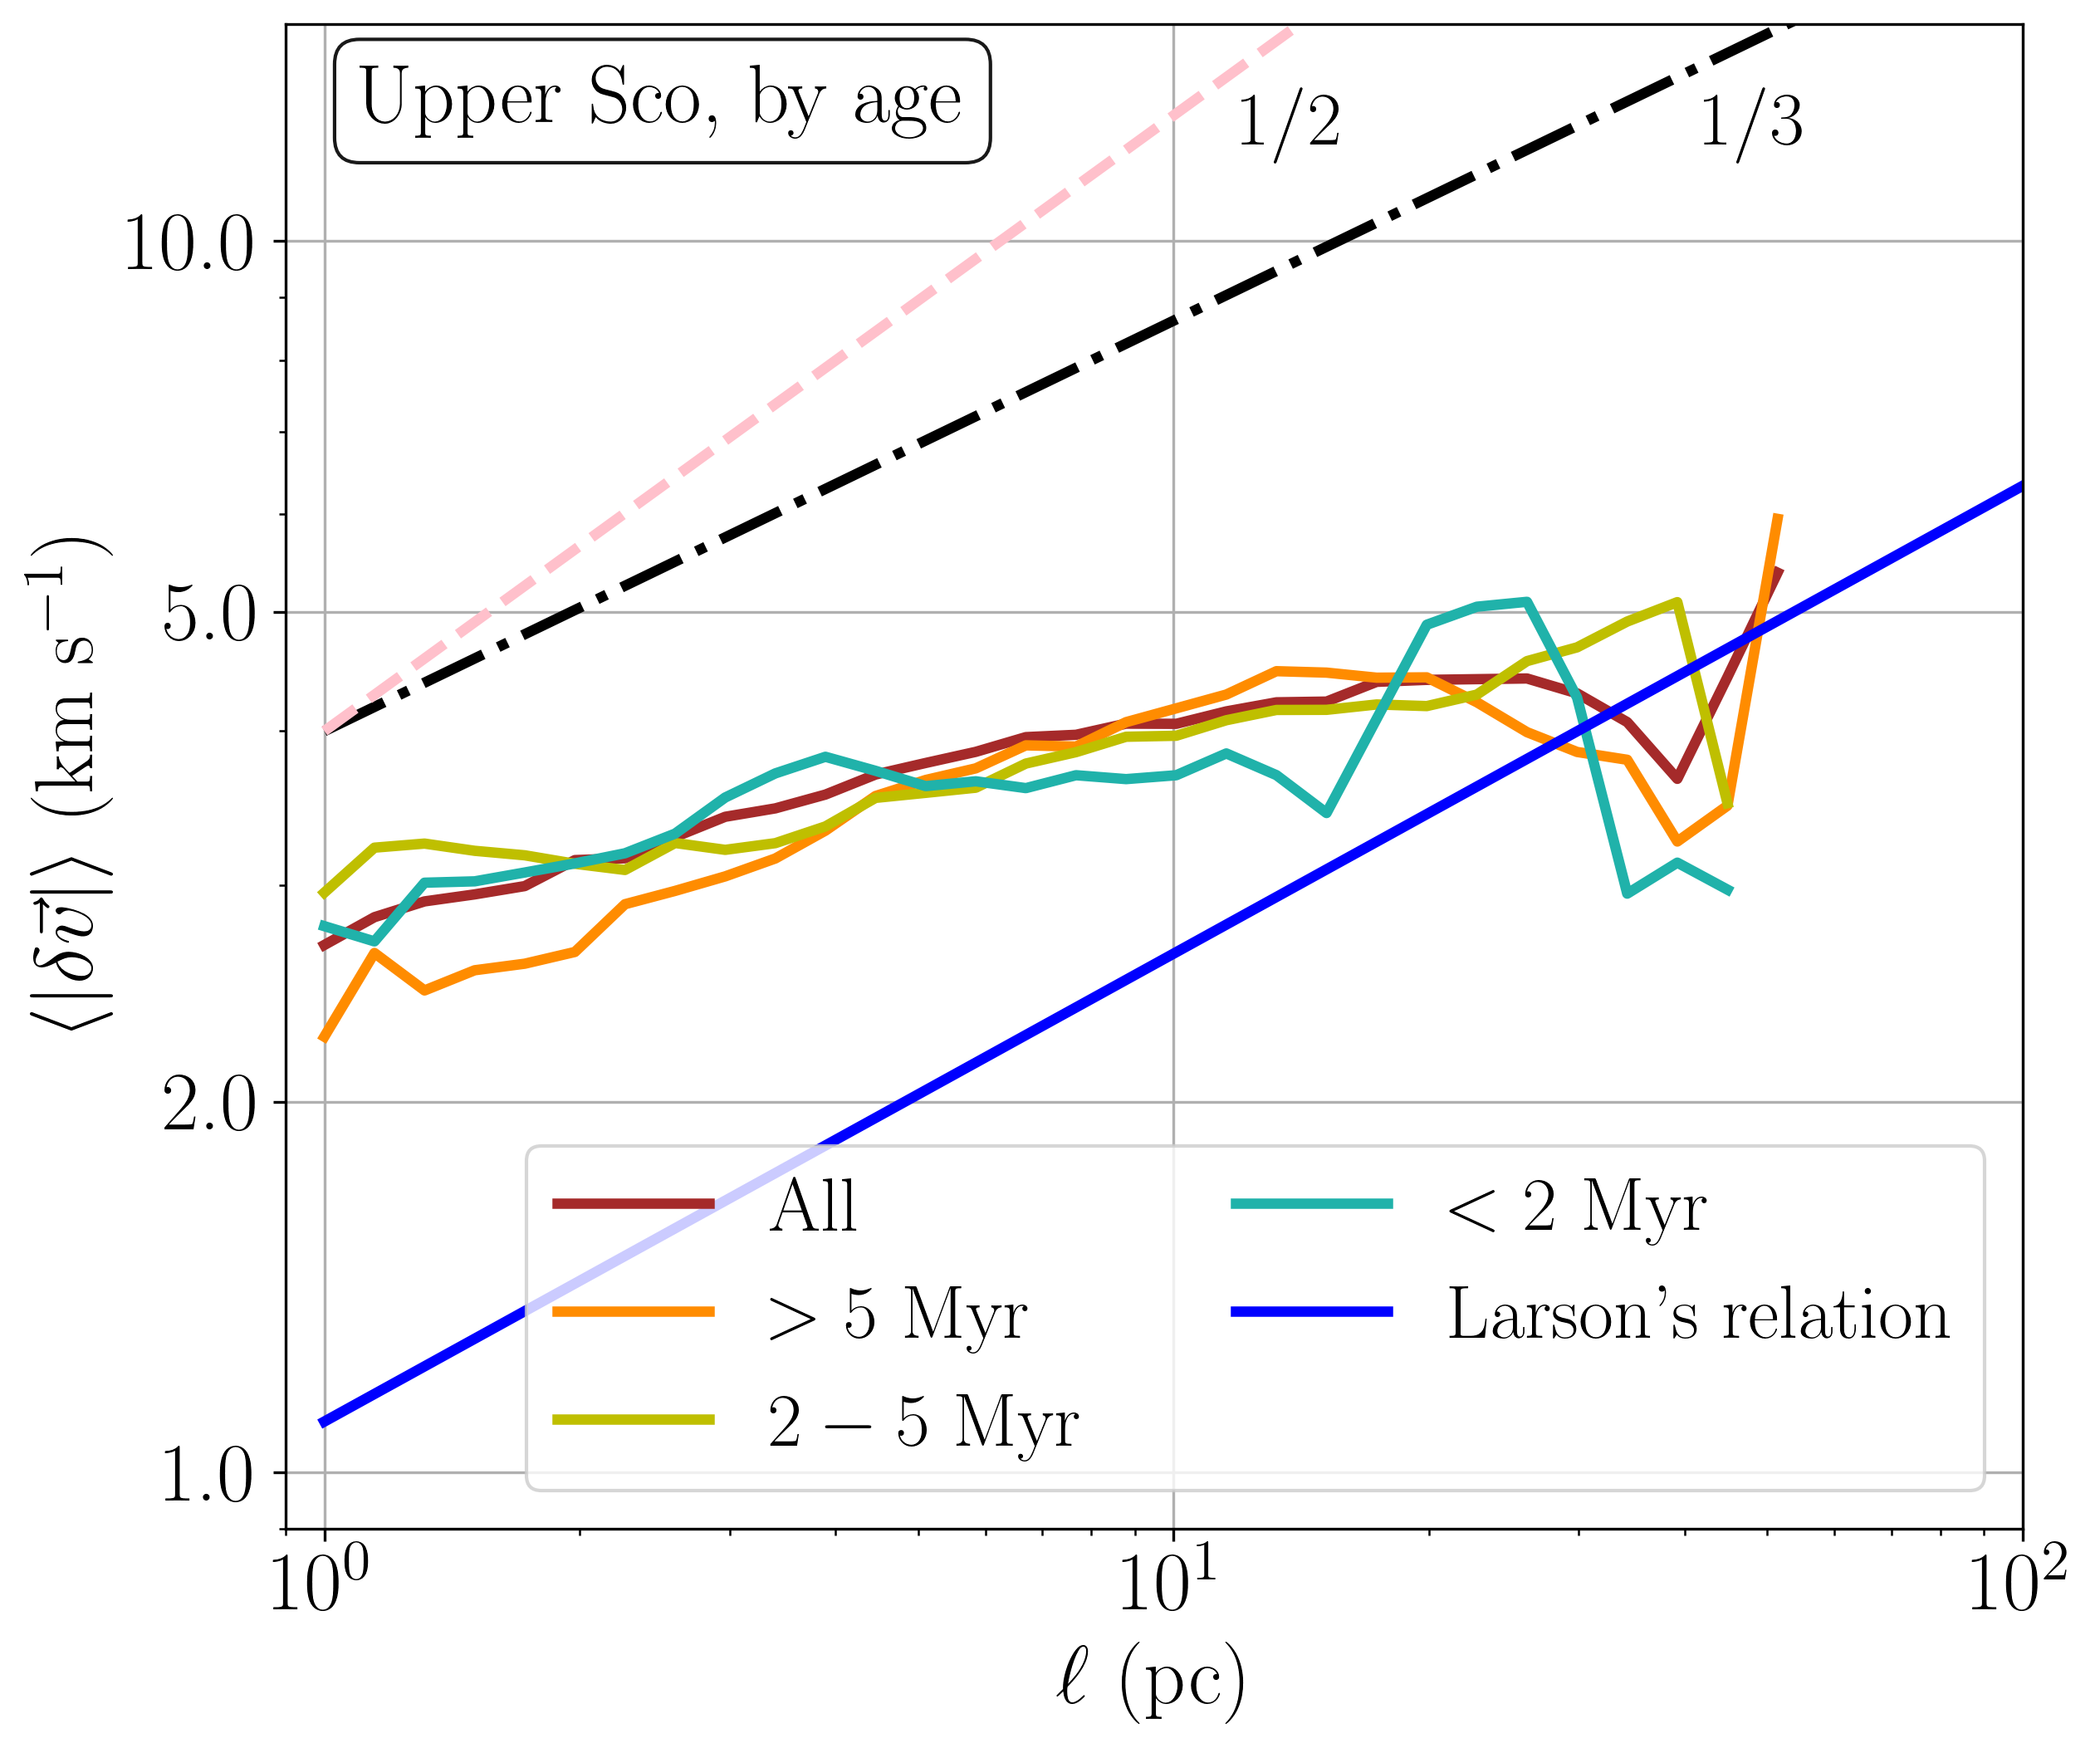
\includegraphics[width=0.7\columnwidth]{Stars_img/UpperSco_age2_vsf.png}
    \caption{Top panel: positions of young stars color-coded by their age. Stellar age is estimated using the Sagitta package developed by \citet{mcbride_untangling_2021}. Background shows \halpha~flux from the WHAM survey. Bottom panel: the VSF of stars in Upper Sco within three age brackets. Only stars younger than 2 Myr show characteristic of SN energy injection.}
    \label{fig:uppersco_age}
\end{figure}
In the main body of this paper, we select only stars within the actively star-forming region Ophiuchus. Here, we show the analysis results when selecting the entire Upper Sco region and discuss how the VSF of the stars depend on the stellar age.

The top panel of Figure \ref{fig:uppersco_age}~shows the spatial distribution of stars in Upper Sco and their age. Most of the stars outside Ophiuchus~are older than 4 Myr, while stars inside Ophiuchus~are much younger, primarily younger than 2 Myr. The SN explosion in this region traced by runaway stars took place $\sim 2$~Myr ago \citep[][]{neuhauser_nearby_2020}, so the majority of stars in Upper Sco did not receive energy injection from this event, and thus would not exhibit characteristics of such energy injection in their VSF\@. Indeed, we see this trend in the lower panel of Figure \ref{fig:uppersco_age}. With the entire Upper Sco region taken into account, the VSF shows only a slight bump at $\sim 25$~pc, while both the VSF of stars older than 5 Myr and of stars between 2 and 5 Myr do not show any discernible energy injection scale. Meanwhile, the VSF of stars younger than 2 Myr shows a clear energy injection scale at $\sim 25$~pc, similar to what we obtain in the main paper. Because of these results, we elect to use only stars categorized as members of Ophiuchus, the majority of which are younger than 1 Myr, for the analysis in the main body of this paper.


\subsubsection{Effect of Galactic Rotation on the VSF of \texorpdfstring{\halpha}{H-alpha}}
\label{sec:rotation}

\begin{figure}
    \centering
    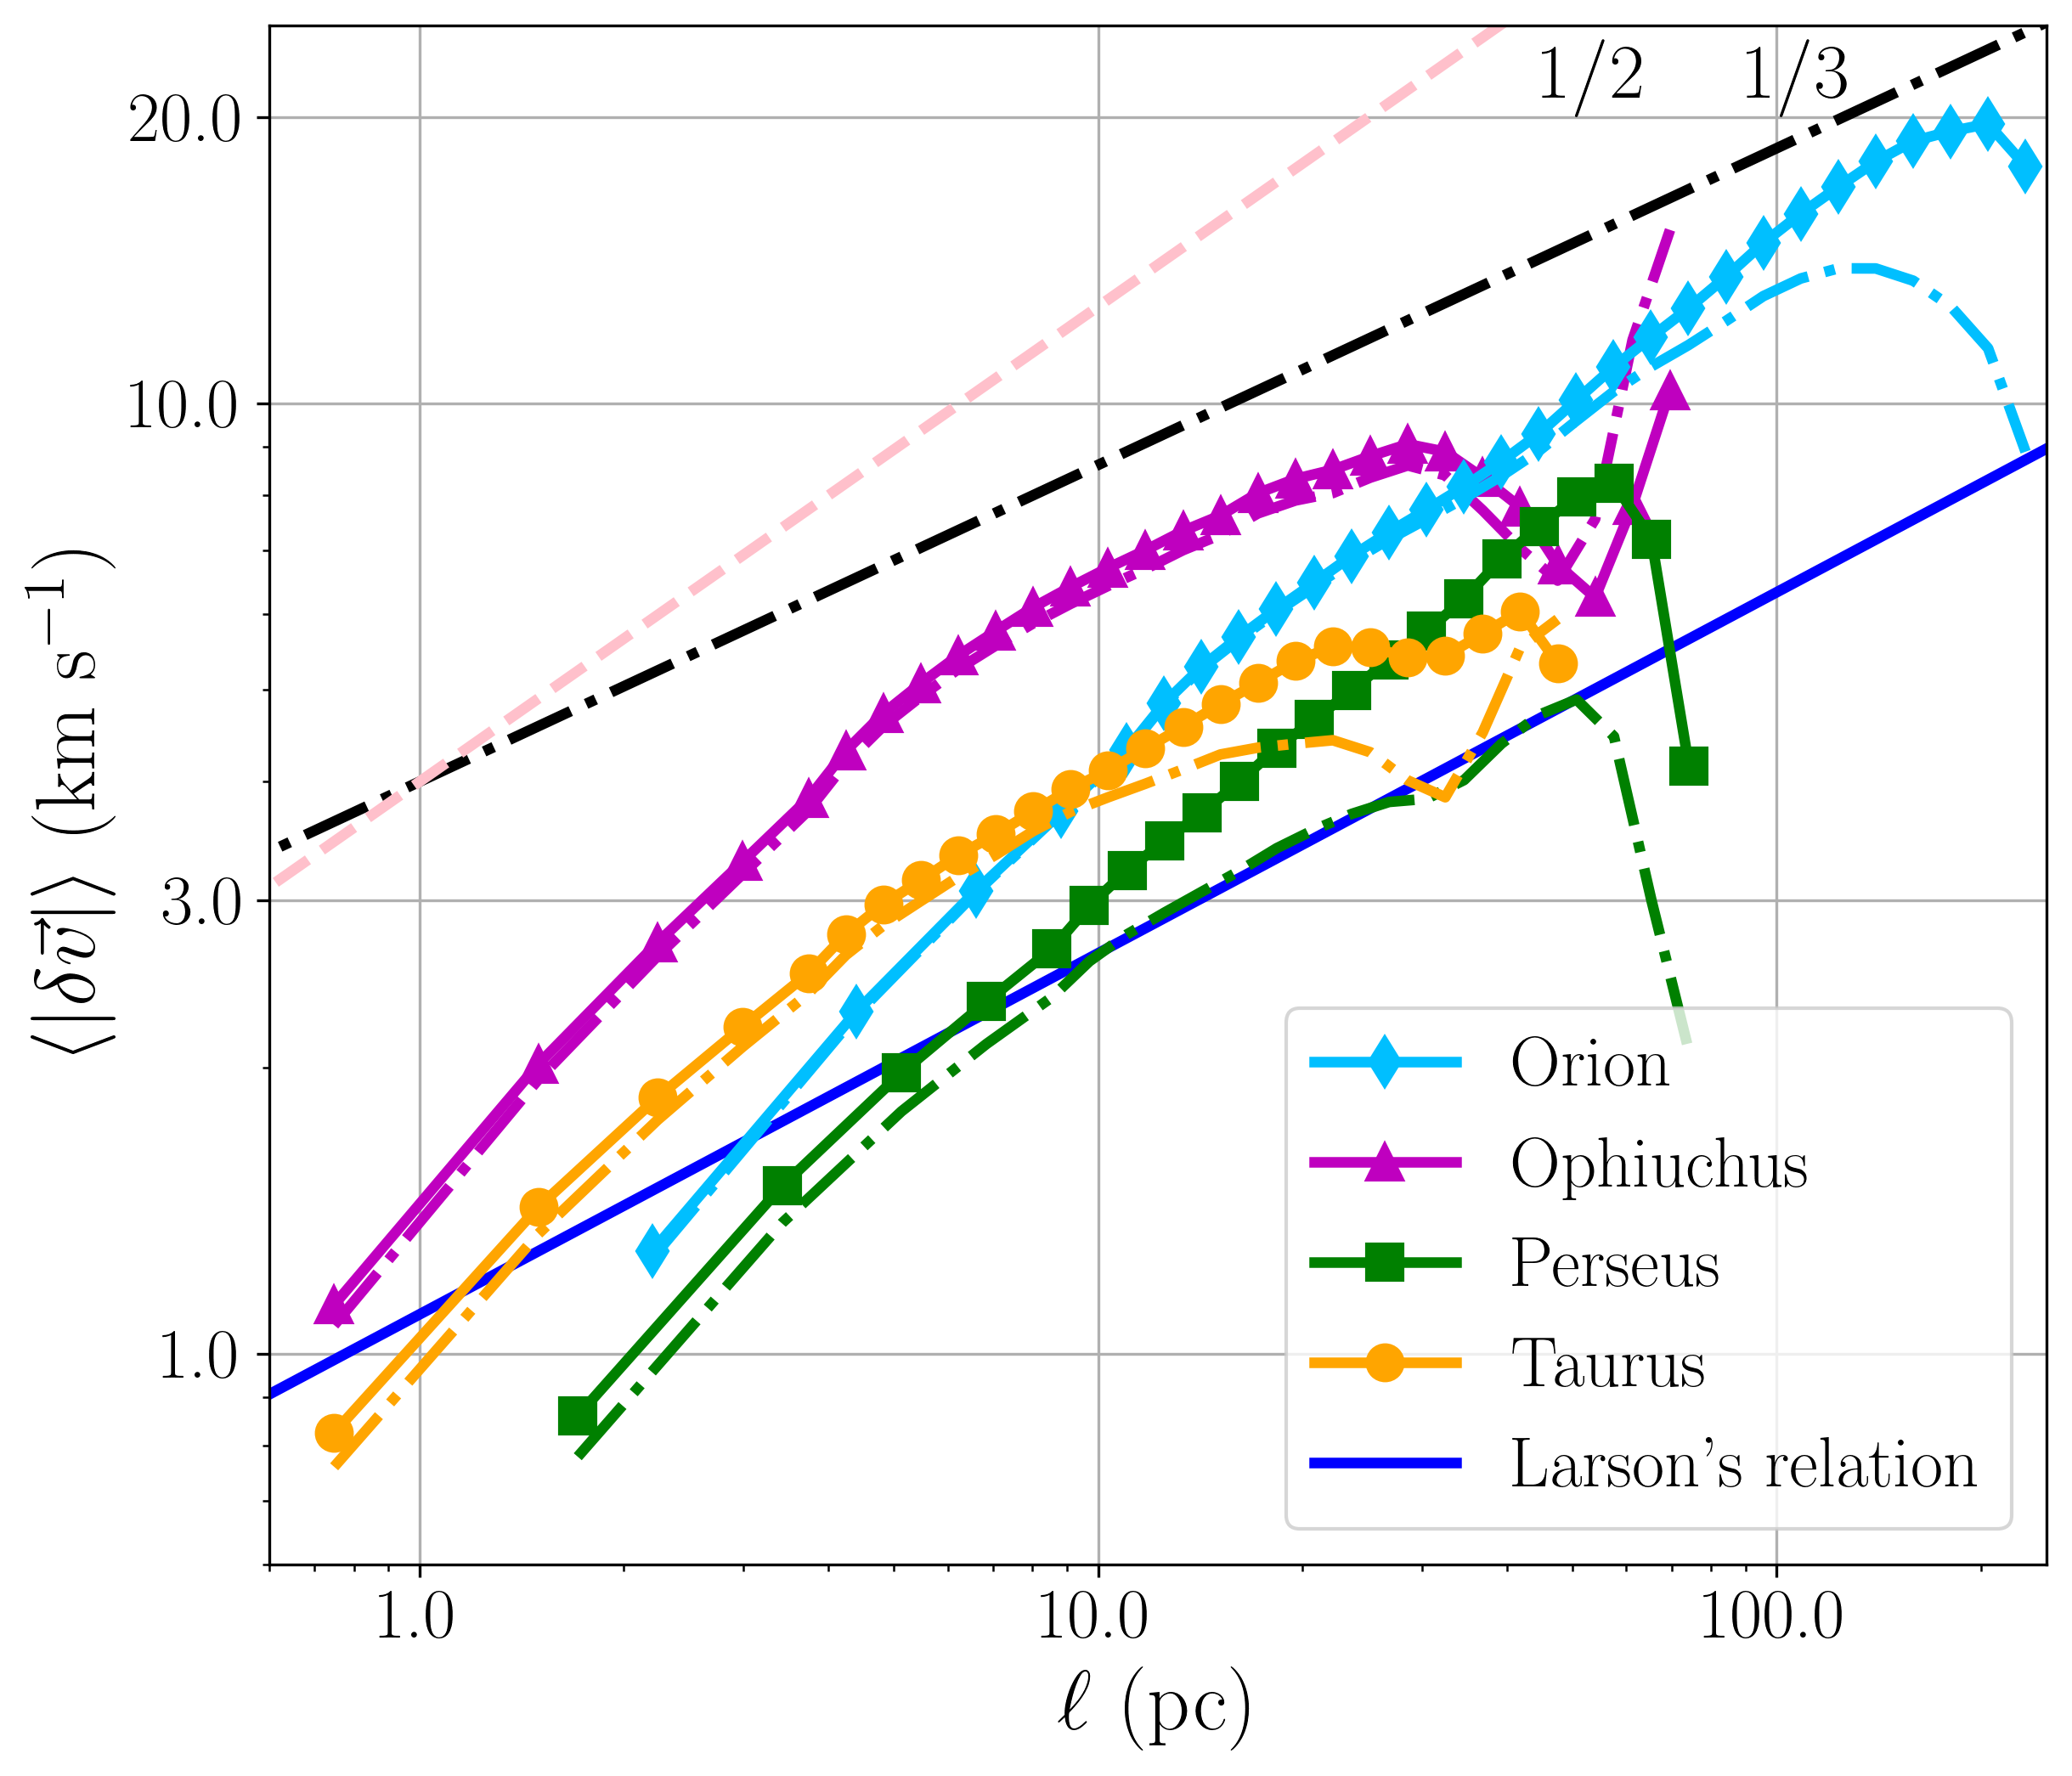
\includegraphics[width=\columnwidth]{Stars_img/test_rotation.png}
    \caption{The VSFs of \halpha, with (solid lines) and without (dotted-dashed lines) a correction to the Galactic rotation \citep{qu_warm_2020}.}
    \label{fig:rotation}
\end{figure}

Figure \ref{fig:rotation} shows the VSF traced by \halpha~in four regions with and without Galactic rotation correction. In three out of the four regions, when a rotation profile is applied, the VSF does not significantly differ from the VSF without a rotation correction up to $\sim 20$~pc. This behavior is expected, since at small $\ell$ the rotation corrections between two points are very similar. Thus, $\delta \vec{v}$ between two points essentially cancels out the rotation correction, and the shape of the VSF is preserved. For two points separated by a large distance, the rotation correction applied to them can differ more, and hence results in a shift in the VSF, as Figure \ref{fig:rotation} shows. However, the overall shifts in the VSFs due to rotation correction are moderate and do not affect the conclusions of our work. 

\subsubsection{Effect of the size and location of the \texorpdfstring{\halpha}{H-alpha}~window}
\label{sec:windowsize}

\begin{figure*}[ht]
    \centering
    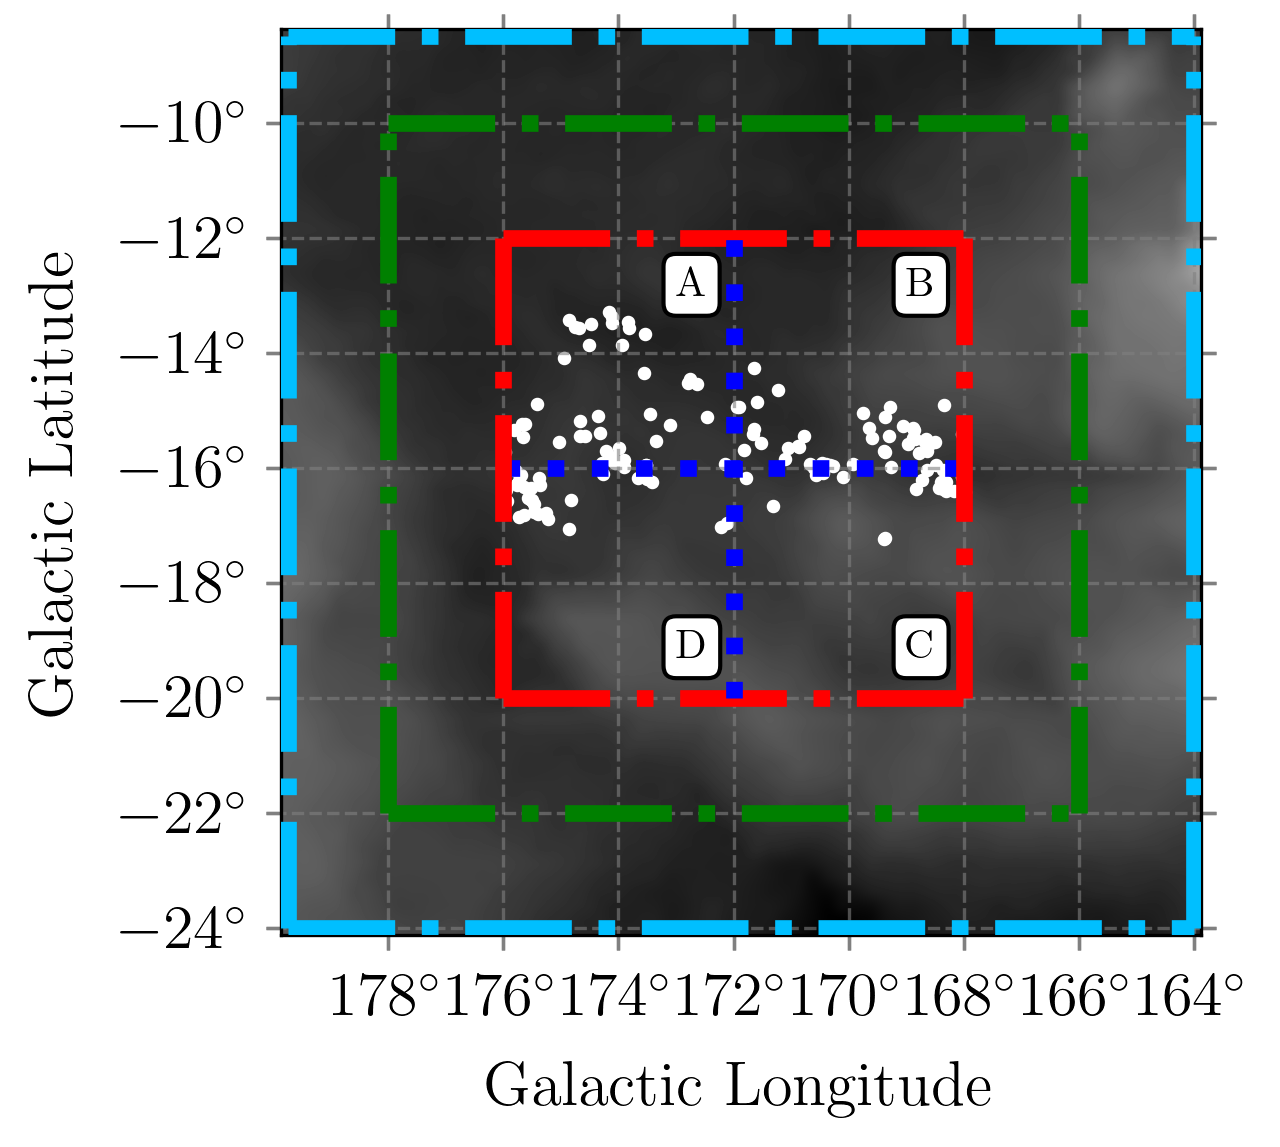
\includegraphics[width=0.5\linewidth]{Stars_img/tau_illustration.png} \\
    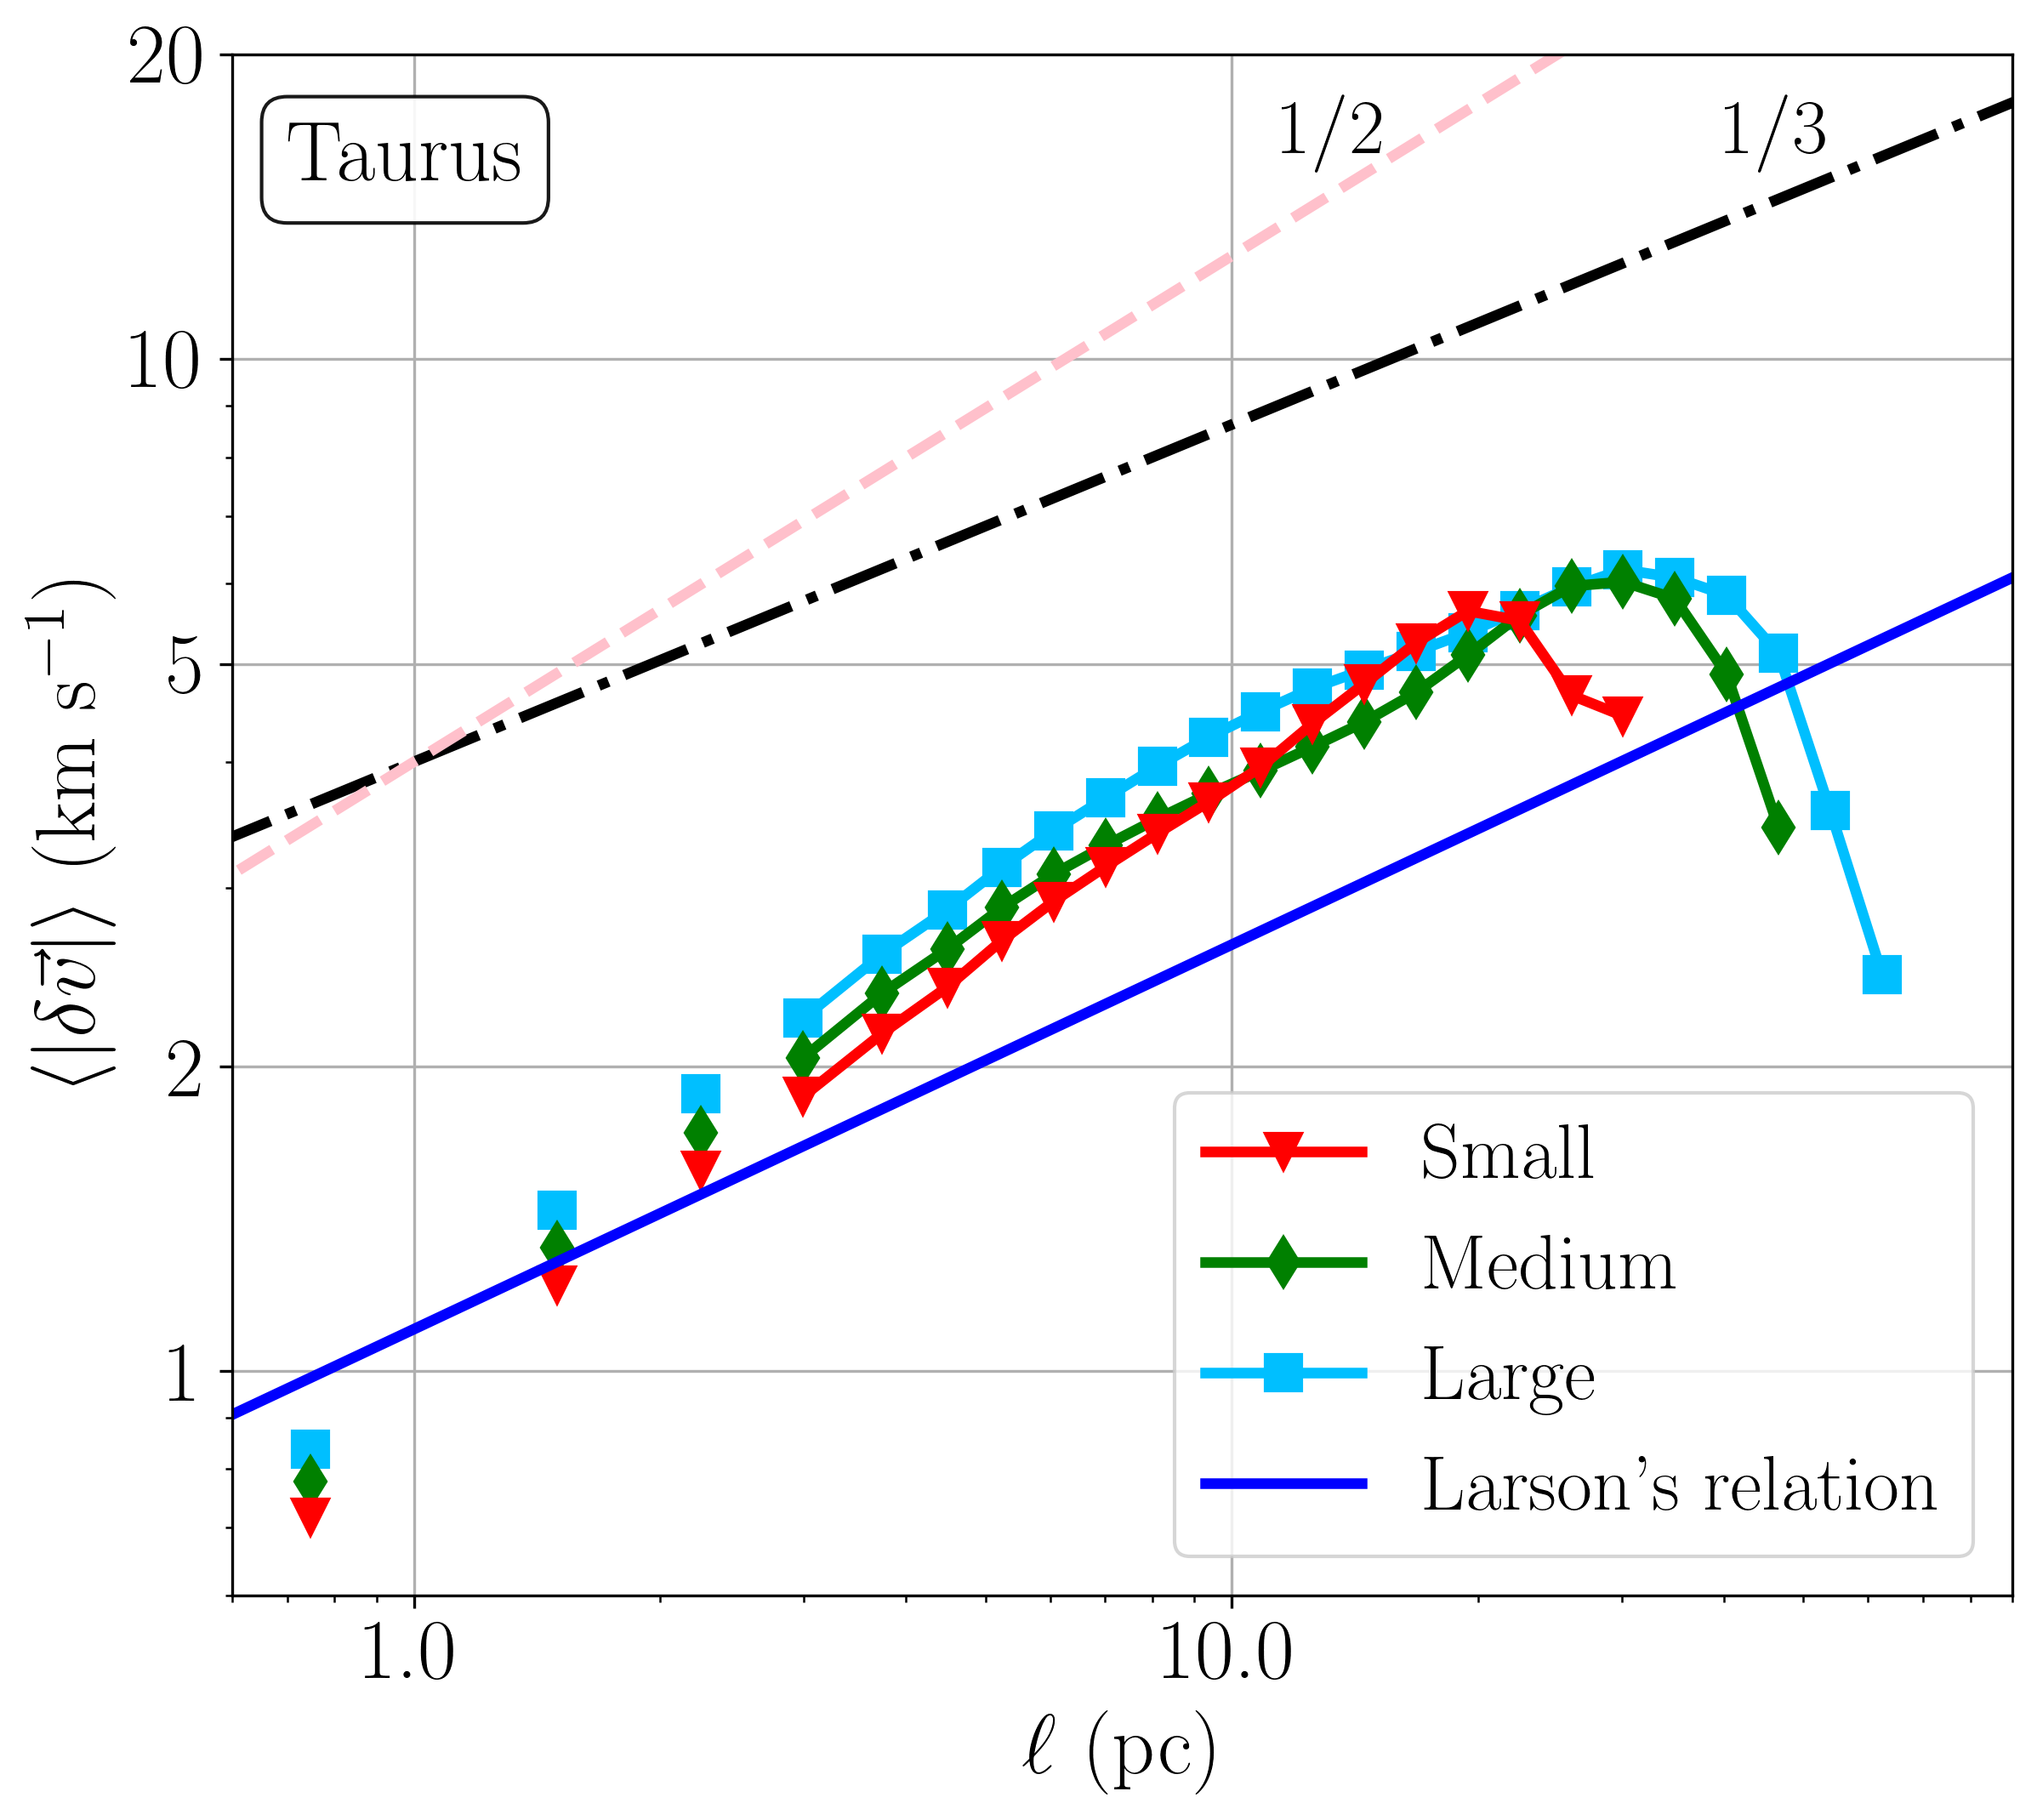
\includegraphics[width=0.45\linewidth]{Stars_img/different_size_test_tau.png}
    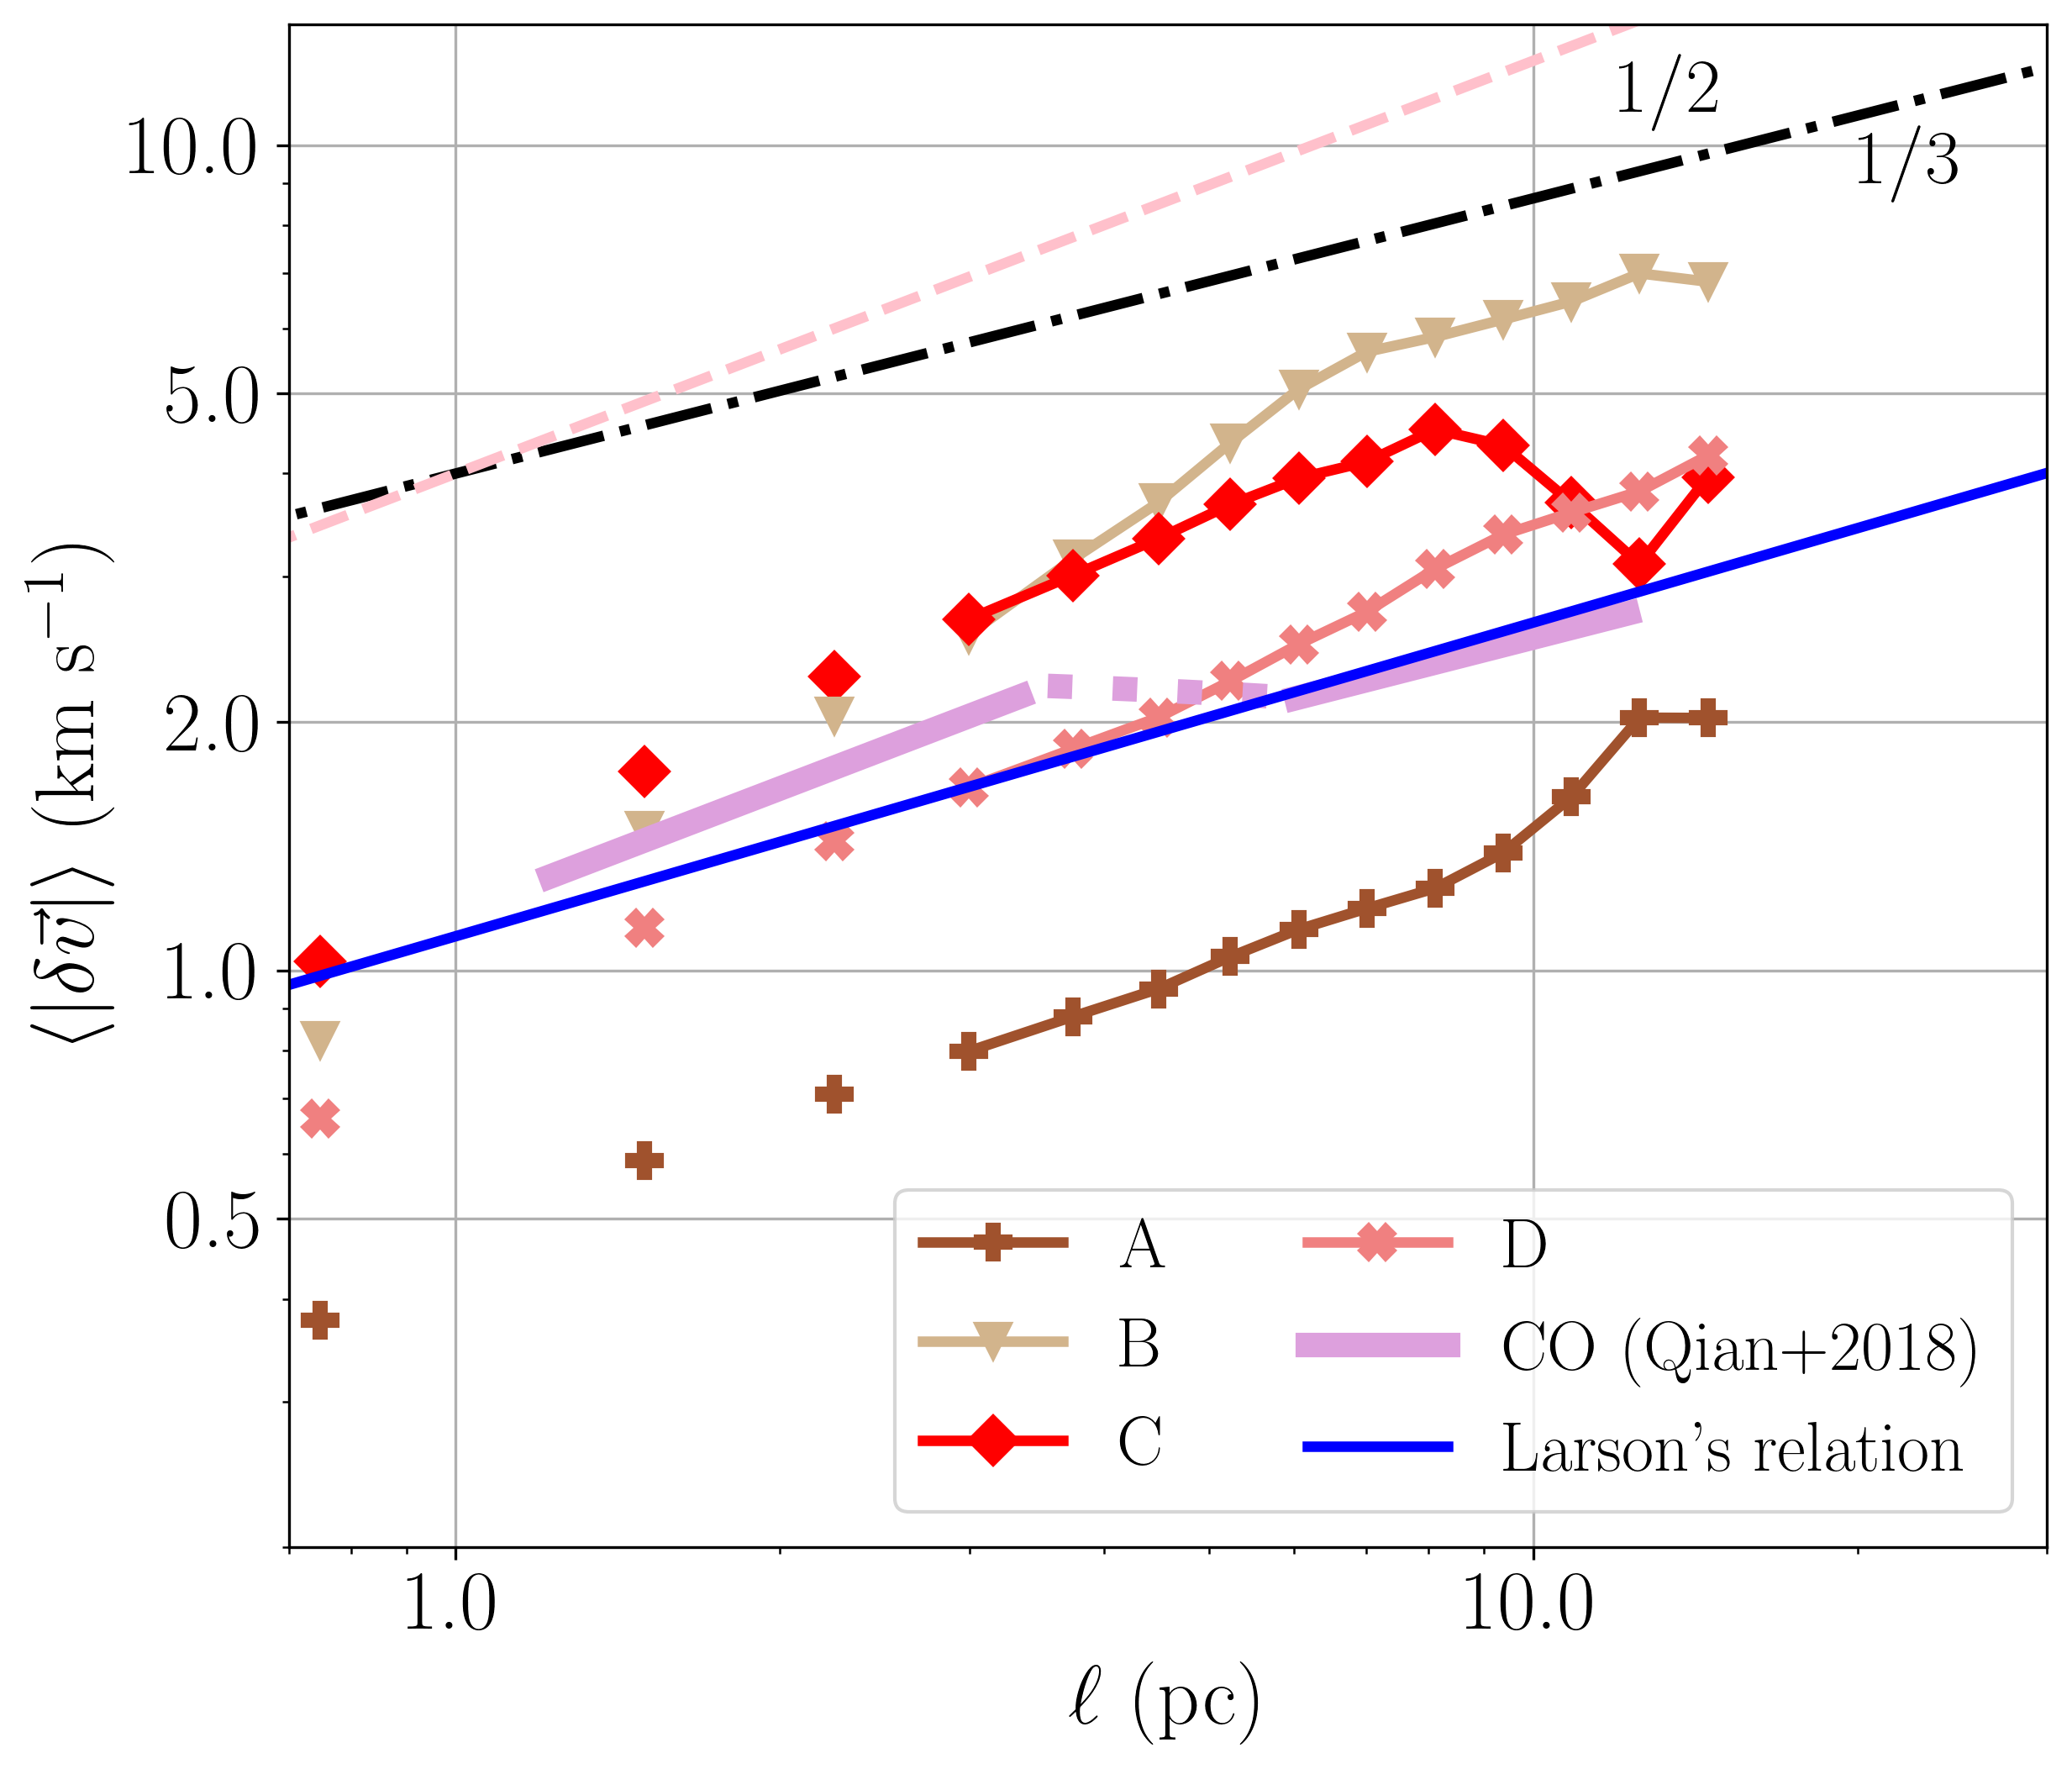
\includegraphics[width=0.46\linewidth]{Stars_img/same_size_test_tau.png}
    \caption{Top panel: illustration of our \halpha~window tests. The red box is the smallest window within which all stars in Taurus belong. The two boxes in green (the window used in the main analysis) and light-blue are each 4 deg$^2$~bigger than the former. Inside the red box, we also test the variation of the VSF within the region by dividing the window into four equal-sized boxes. Bottom left panel: The VSF of Taurus traced by \halpha, plotted across three different window sizes.
    Bottom right panel: The \halpha~VSFs of Taurus in the four quadrants within the red window. }
    \label{fig:aperturesize}
\end{figure*}

Another potential source of bias comes from the exact size and location of the window chosen to calculate the VSF of \halpha~within each region. In Section \ref{subset:eachregion_result}, we caution that the bumps seen in the VSF of \halpha~are potential artifacts since they are close to the size of the window. Such an effect is noted as the apparent driving scale in simulations of multiphase turbulence, and is equal to 1/2 of the box size \citep[e.g.,][]{mohapatra_velocity_2022}. To test whether this effect is also present in the VSF of \halpha, we select a solid angle that encompasses all the stars in a region, and compute the VSF within this window. We then compute the VSF for a window that is 4 deg$^2$ larger, and repeat this a second time (see top panel in Figure~\ref{fig:aperturesize}).

In all four regions, the VSFs of \halpha~are independent of the window size up to $\ell \sim L/2$, where $L$ is the window size. In Taurus and Perseus, the bump in the VSF shifts to larger $\ell$ when the window size increases. Thus we conclude that in these regions, the VSF bump is likely caused by the box limit rather than a real physical driving scale. As an example, the bottom left panel of Figure \ref{fig:aperturesize} shows the VSF of \halpha~in Taurus as a function of window size. 



We also use Taurus as an example to illustrate the spatial variation of turbulence on small scales. We divide the smallest box (8 deg$^2$) in the previous experiment into four equal-sized quadrants. The bottom right panel of Figure \ref{fig:aperturesize} shows the \halpha~ VSFs of these four quadrants in Taurus. Although the slopes of these four VSFs are roughly consistent with one another, their amplitudes vary by up to a factor of three, indicating potentially large variations in turbulence between local patches of the ISM\@. The VSF of CO is in the best agreement with the bottom-left window ($172^{\circ} < l < 176^{\circ}$~and $-20^{\circ} < b < -16^{\circ}$), where many CO cores were also identified \citep[see Figure 2 of][for detailed locations of CO cores in Taurus]{qian_13co_2012}.

\chapter{\texorpdfstring{\MakeUppercase{Machine Learning Characterization of Intermittency in Plasma Turbulence}}{Machine Learning Characterization of Intermittency in Plasma Turbulence}} \label{chap:ml}

The classical theory of turbulence assumes that the energy transfer mechanism is volumetric and self-similar \citep{kolmogorov_local_1941}---that is, the shape of the turbulent eddies is identical on all scales $\ell < \ell_0$ within the inertial range.
However, experiments and numerical simulations have demonstrated that some structures in this flow become increasingly sparse in time and space as $\ell$ decreases \citep{she_universal_1994,zhdankin_statistical_2013};
their distributions also become prominently non-Gaussian, especially when a strong, fluctuating magnetic field is introduced.
These spatio-temporal fluctuations of the turbulent flow are broadly classified as \emph{intermittency}.

\begin{figure}[htbp]
    \centering
    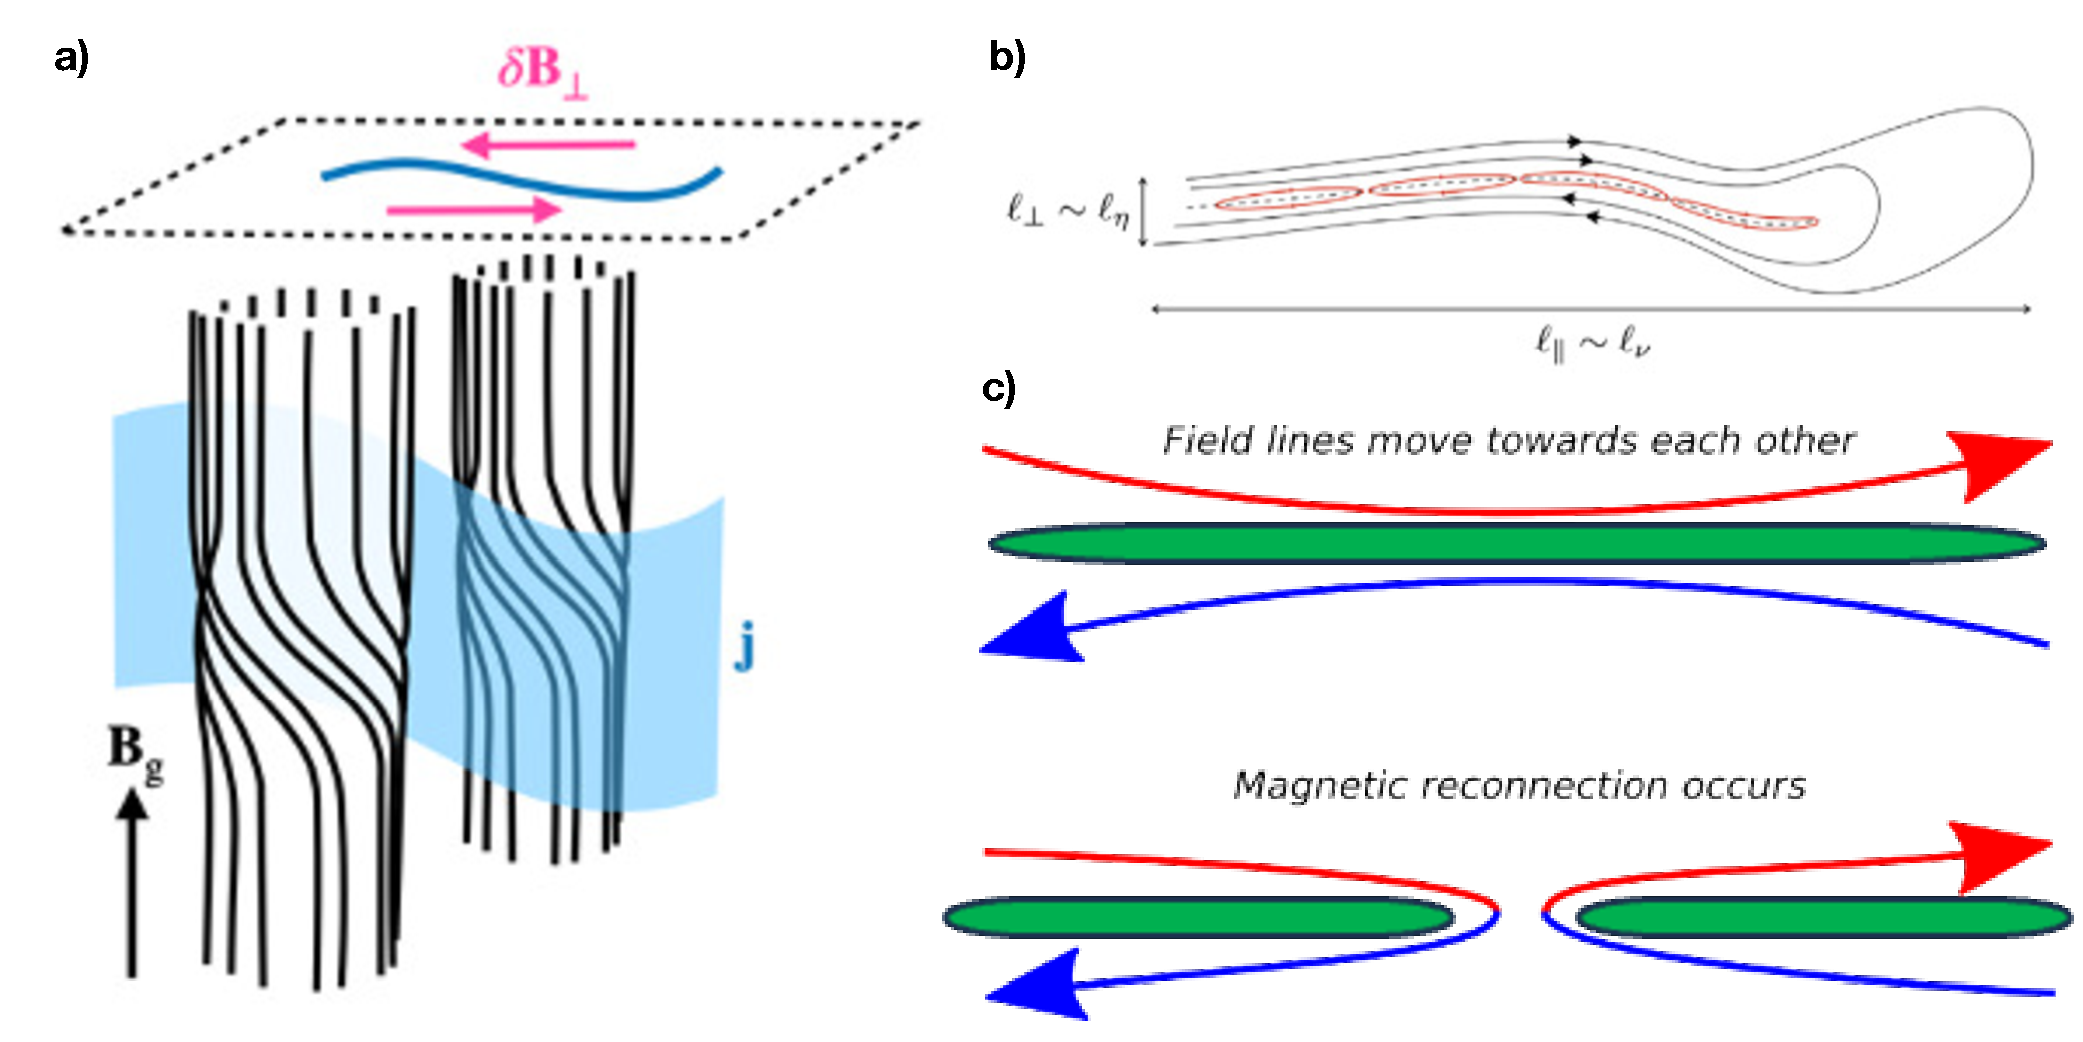
\includegraphics[width=0.8\linewidth]{Plasma_img/current_sheet_illustration.pdf}
    \caption{Illustration of a current sheet in the classical picture.\\ a) A current sheet formed by a local twist in the direction of the in-plane magnetic field, which induces a current density moving upward. Credit: Joonas Nättilä.\\ b) A top-down view showing folded magnetic field lines, resulting in the formation of a current sheet (red contours) at the boundary. Adapted from \citet[][]{galishnikova_tearing_2022}.\\ c) Current sheets can undergo tearing-mode instability, which creates a hole in the surface where magnetic field lines can cross and ``reconnect'' with the other side, resulting in violent dissipation of magnetic energy.}
    \label{fig:current-sheets}
\end{figure}

A manifestation of intermittency in magnetically dominated environments arises in the form of a ``current sheet''---a two-dimensional surface of plasma with very high current densities \citep[][]{zhou_spectrum_2023}.
In the accepted framework of plasma turbulence, current sheets form when there is a local reversal in the magnetic polarity across a boundary, resulting in a strong induced current in a thin sheet. See Figure~\ref{fig:current-sheets} for additional visual illustrations of this phenomenon.

Current sheets can undergo tearing-mode instability and break apart \citep[e.g.,][]{loureiro_instability_2007,galishnikova_tearing_2022}, leaving ``holes'' in the boundary where magnetic field lines can cross and reconnect with field lines pointing in the opposite direction---a phenomenon known as \textit{magnetic reconnection}.
Reconnection allows a sudden conversion of magnetic energy into thermal energy (heating of the plasma) and kinetic energy (non-thermal acceleration of particles) via the Fermi process \citep[see, e.g.,][]{priest_magnetic_2000}.
Relativistic magnetic reconnection is an efficient channel for converting magnetic energy into high-energy non-thermal particles, as demonstrated in particle-in-cell simulations and summarized in subsequent reviews \citep{sironi_relativistic_2014,kagan_relativistic_2015}.
Thus, identifying current sheets and analyzing their statistics is of great interest to both the field of high-energy astrophysics and solar physics.

In \citet[][]{ha_machine_2025}, we employ a theory-agnostic approach to characterizing intermittency (i.e., current sheets) in magnetically dominated pair-plasma turbulence.
Namely, we use a machine-learning (ML) technique, the self-organizing map \citep[SOM,][]{kohonen_self-organizing_1990}, to identify structures consistent with current sheets in three kinetic plasma simulations.
Intermittent structures in plasma turbulence have previously been identified by thresholding current densities \citep{zhdankin_statistical_2013} and by using Gaussian-fitting techniques \citep{greco_statistical_2009}.
Other attempts have been made to detect current sheets using various supervised and unsupervised ML methods \citep[e.g.,][]{hu_identifying_2020,sisti_detecting_2021,bussov_maarja_segmentation_2021,kohne_unsupervised_2023, edmond_clustering_2024}.
These studies offer a promising outlook on the usability of novel computational methods to identify, in particular, current sheets in two-dimensional (2D) simulations and in magnetospheric observations.
Our study is the first of its kind that applies such a technique to 3D simulations of strongly magnetized, relativistic plasma turbulence.

The following sections are adapted from \citet{ha_awesom_2025}, the Journal of Open Source Software, 10, 7613, and \citet{ha_machine_2025}, the Astrophysical Journal Letters, 985, L31.

\section{aweSOM: A GPU-accelerated Clustering Algorithm for Anomaly Detection}

\publicationdetailsnoabstract
{Ha et al.\ 2025, JOSS, 10, 7613}
{Trung Ha\footnotemark[1]\footnotemark[2]\footnotemark[3], Joonas Nättilä\footnotemark[4]\footnotemark[5]\footnotemark[2], and Jordy Davelaar\footnotemark[6]\footnotemark[7]\footnotemark[2]\footnotemark[5]}
{\footnotetext[1]{Department of Astronomy, University of Massachusetts-Amherst, Amherst, MA 01003, USA}
\footnotetext[2]{Center for Computational Astrophysics, Flatiron Institute, 162 Fifth Avenue, New York, NY 10010, USA}
\footnotetext[3]{Department of Physics, University of North Texas, Denton, TX 76203, USA}
\footnotetext[4]{Department of Physics, University of Helsinki, P.O. Box 64, University of Helsinki, FI-00014, Finland}
\footnotetext[5]{Physics Department and Columbia Astrophysics Laboratory, Columbia University, 538 West 120th Street, New York, NY 10027, USA}
\footnotetext[6]{Department of Astrophysical Sciences, Peyton Hall, Princeton University, Princeton, NJ 08544, USA}
\footnotetext[7]{NASA Hubble Fellowship Program, Einstein Fellow}}
\setcounter{footnote}{0}

\subsection{Summary}

We introduce \awesom, an open-source Python package for machine learning (ML) clustering and classification, using a self-organizing map \citep[SOM,][]{kohonen_self-organizing_1990} algorithm that incorporates CPU/GPU acceleration to accommodate large ($N > 10^6$, where $N$ is the number of data points), multi-dimensional datasets. \awesom\ consists of two main modules, one that handles the initialization and training of the SOM, and another that stacks the results of multiple SOM realizations to obtain more statistically robust clusters.

Existing Python-based SOM implementations (e.g., \texttt{POPSOM}, \citet{yuan_implementation_2018}; \texttt{MiniSom}, \citet{vettigli_minisom_2018}; \texttt{sklearn-som}) primarily serve as proof-of-concept demonstrations, optimized for smaller datasets, but lacking scalability for large, multi-dimensional data.
\awesom\ provides a solution for this gap in capability, with good performance scaling up to $\sim 10^8$ individual points, and capable of utilizing multiple features per point. We compare the code performance against the legacy implementations it is based on, and find a $10\text{--}100\times$ speedup, as well as significantly improved memory efficiency, due to several built-in optimizations.

As a companion to this paper, \citet{ha_machine_2025} demonstrates the capabilities of \awesom\ in analyzing the physics of plasma turbulence. Detailed instructions on how to install, test, and replicate the results of the paper are available in the online \href{https://awesom.readthedocs.io/en/latest/}{documentation}. Also included in the documentation is an example of applying \awesom\ to the Iris dataset \citep{fisher_iris_1936}.

\subsection{Statement of need}

\subsubsection{The self-organizing map algorithm}

A SOM algorithm is an unsupervised ML technique that excels at dimensionality reduction, clustering, and classification tasks.
It consists of a 2-dimensional (2D) lattice of nodes. Each node contains a weight vector that matches the dimensionality of the input data. A SOM performs clustering by adapting the weight vectors of nodes, progressively reshaping the lattice’s topology to match the intrinsic clustering of the input data.
In this manner, a SOM lattice can capture multi-dimensional correlations in the input data.

SOM is commonly used in various real-world applications, such as in the financial sector \citep[e.g.,][]{alshantti_self-organising_2021,pei_financial_2023}, in environmental surveys \citep[e.g.,][]{alvarez-guerra_assessment_2008, li_using_2020}, in medical technology \citep[e.g.,][]{hautaniemi_analysis_2003,kawaguchi_electroencephalogram-based_2024}, among others. \awesom\ was originally developed to be used in analyzing astrophysical simulations, but can be applied to a wide variety of real-world scientific data sets.

\centerline{\textbf{\texttt{POPSOM}}}

We base the SOM module of \awesom\ on \texttt{POPSOM} \citep{yuan_implementation_2018, hamel_vsom_2019}, a R-based SOM model. \popsom\ was developed as a single-threaded, stochastic training algorithm with built-in visualization capabilities. However, due to its single-threaded nature, the algorithm does not scale well with large datasets. When $N \gtrsim 10^6$, \popsom\ is often unable to complete the training process as the dimensionality of the input data increases due to its much higher memory usage. As an example, we generated a mock dataset with $N = 10^6$ and $F = 6$ dimensions, then trained it on a lattice of $X = 63$, and $Y = 32$, where $X, Y$ are the dimensions of the lattice, using one Intel Icelake node with 64 cores and 1 TB memory. \popsom\ completed the training in $\approx 2200$ s and consumed $\approx 600$ GB of system memory at its peak.

\centerline{\textbf{Rewriting \popsom\ into \awesom}}

To combat the long training time and excessive memory usage, we rewrite \popsom\ with multiple optimizations/parallelizations.
We replaced legacy code with modern \texttt{NumPy} functions for updating the lattice (a 3D array) and eliminated the use of \texttt{Pandas} DataFrames \citep{the_pandas_development_team_pandas-devpandas_2024}, which consume significantly more memory. The weight vector modifications in the DataFrame were also less efficient compared to the NumPy arrays used in aweSOM\@.
Furthermore, for the steps where parallelization could be leveraged (such as when the cluster labels are mapped to the lattice, then to the input data), we integrate \texttt{Numba} \citep{lam_numba_2015} to take advantage of its Just-In-Time (JIT) compiler and simple parallelization of loops. In the same example as above, \awesom\ took $\approx 200$ s and consumed $\approx 450$ MB of memory to complete the training and clustering. In addition to the $\sim 10 \times$ speedup, \awesom\ is also $\sim 10^3 \times$ more memory-efficient.

The left hand side of \autoref{fig:sce_scaling} shows a graph of the performance between \awesom\ and the legacy \popsom\ implementation over a range of $N$ and $F$, performed on one Intel Icelake compute node with 64 CPU cores and 1 TB memory.
While \popsom\ initially performs slightly faster than \awesom\ for $N \lesssim 10^4$, this changes when $N$ exceeds $5 \times 10^5$; after that, \awesom\ consistently outperforms \popsom\ by approximately a factor of $10$.
Critically, \popsom\ fails to complete its cluster mapping for $N \gtrsim 10^6, F > 4$ because the memory buffer of the test node was exceeded.

\subsubsection{The statistically combined ensemble method}

The statistically combined ensemble (SCE) method was developed by \citet{bussov_maarja_segmentation_2021} to stack the result of multiple independent clustering realizations into a statistically significant set of clusters. This method represents a form of ensemble learning. Additionally, SCE can also be used independently from the base SOM algorithm, and is compatible with any general unsupervised classification algorithm.

\centerline{\textbf{The legacy SCE implementation}}

In its original version, the SCE was saved as a nested dictionary of boolean arrays, each of which contains the spatial similarity index $g$ between cluster $C$ and cluster $C'$. The total number of operations scales as $N_{C}^R$, where $N_C$ is the number of clusters in each realization, and $R$ is the number of realizations. For example, in our use case involving plasma simulation data \citep{ha_machine_2025}, each SOM realization produces on average 7 clusters, and the SCE analysis incorporates 36 realizations, resulting in approximately $7^{36} \sim 10^{30}$ array-to-array comparisons.

\centerline{\textbf{Integrating SCE into \awesom\ with \texttt{JAX}}}

To mitigate this bottleneck, we rewrite the legacy SCE code with \texttt{JAX} \citep{bradbury_jax_2018} to significantly enhance the performance of array-to-array comparisons (which are matrix multiplications) by leveraging the GPU's parallel-computing advantage over the CPU\@. We implement this optimization by replacing the original nested dictionaries with data arrays. Then, every instance of matrix operation using \texttt{numpy} is converted to \texttt{jax.numpy}. Additionally, we implement internal checks such that the SCE code automatically reverts to \texttt{NumPy} if GPU-accelerated \texttt{JAX} is not available.

Similar to the SOM implementation, the SCE implementation in \awesom\ demonstrates excellent scalability as the number of data points increases.
The right hand side of \autoref{fig:sce_scaling} shows a graph of the performance between the two implementations given $R = 20$. At $N < 5 \times 10^4$, the legacy code is faster due to the overhead from loading \texttt{JAX} and the JIT compiler. However, \awesom\ quickly exceeds the performance of the legacy code, and begins to approach its maximum speed-up of $\sim 100 \times$ at $N \gtrsim 10^7$ (performed on one NVIDIA A100-40GB GPU)\@. On the other hand, when running on CPU-only with \texttt{NumPy}, \awesom\ consistently shows a $2 \times$ speed improvement over the legacy code. Altogether, it is best to use \awesom\ with \texttt{NumPy} when $N \lesssim 10^5$, and with \texttt{JAX} when $N \gtrsim 10^5$.

\begin{figure}[htbp]
    \centering
    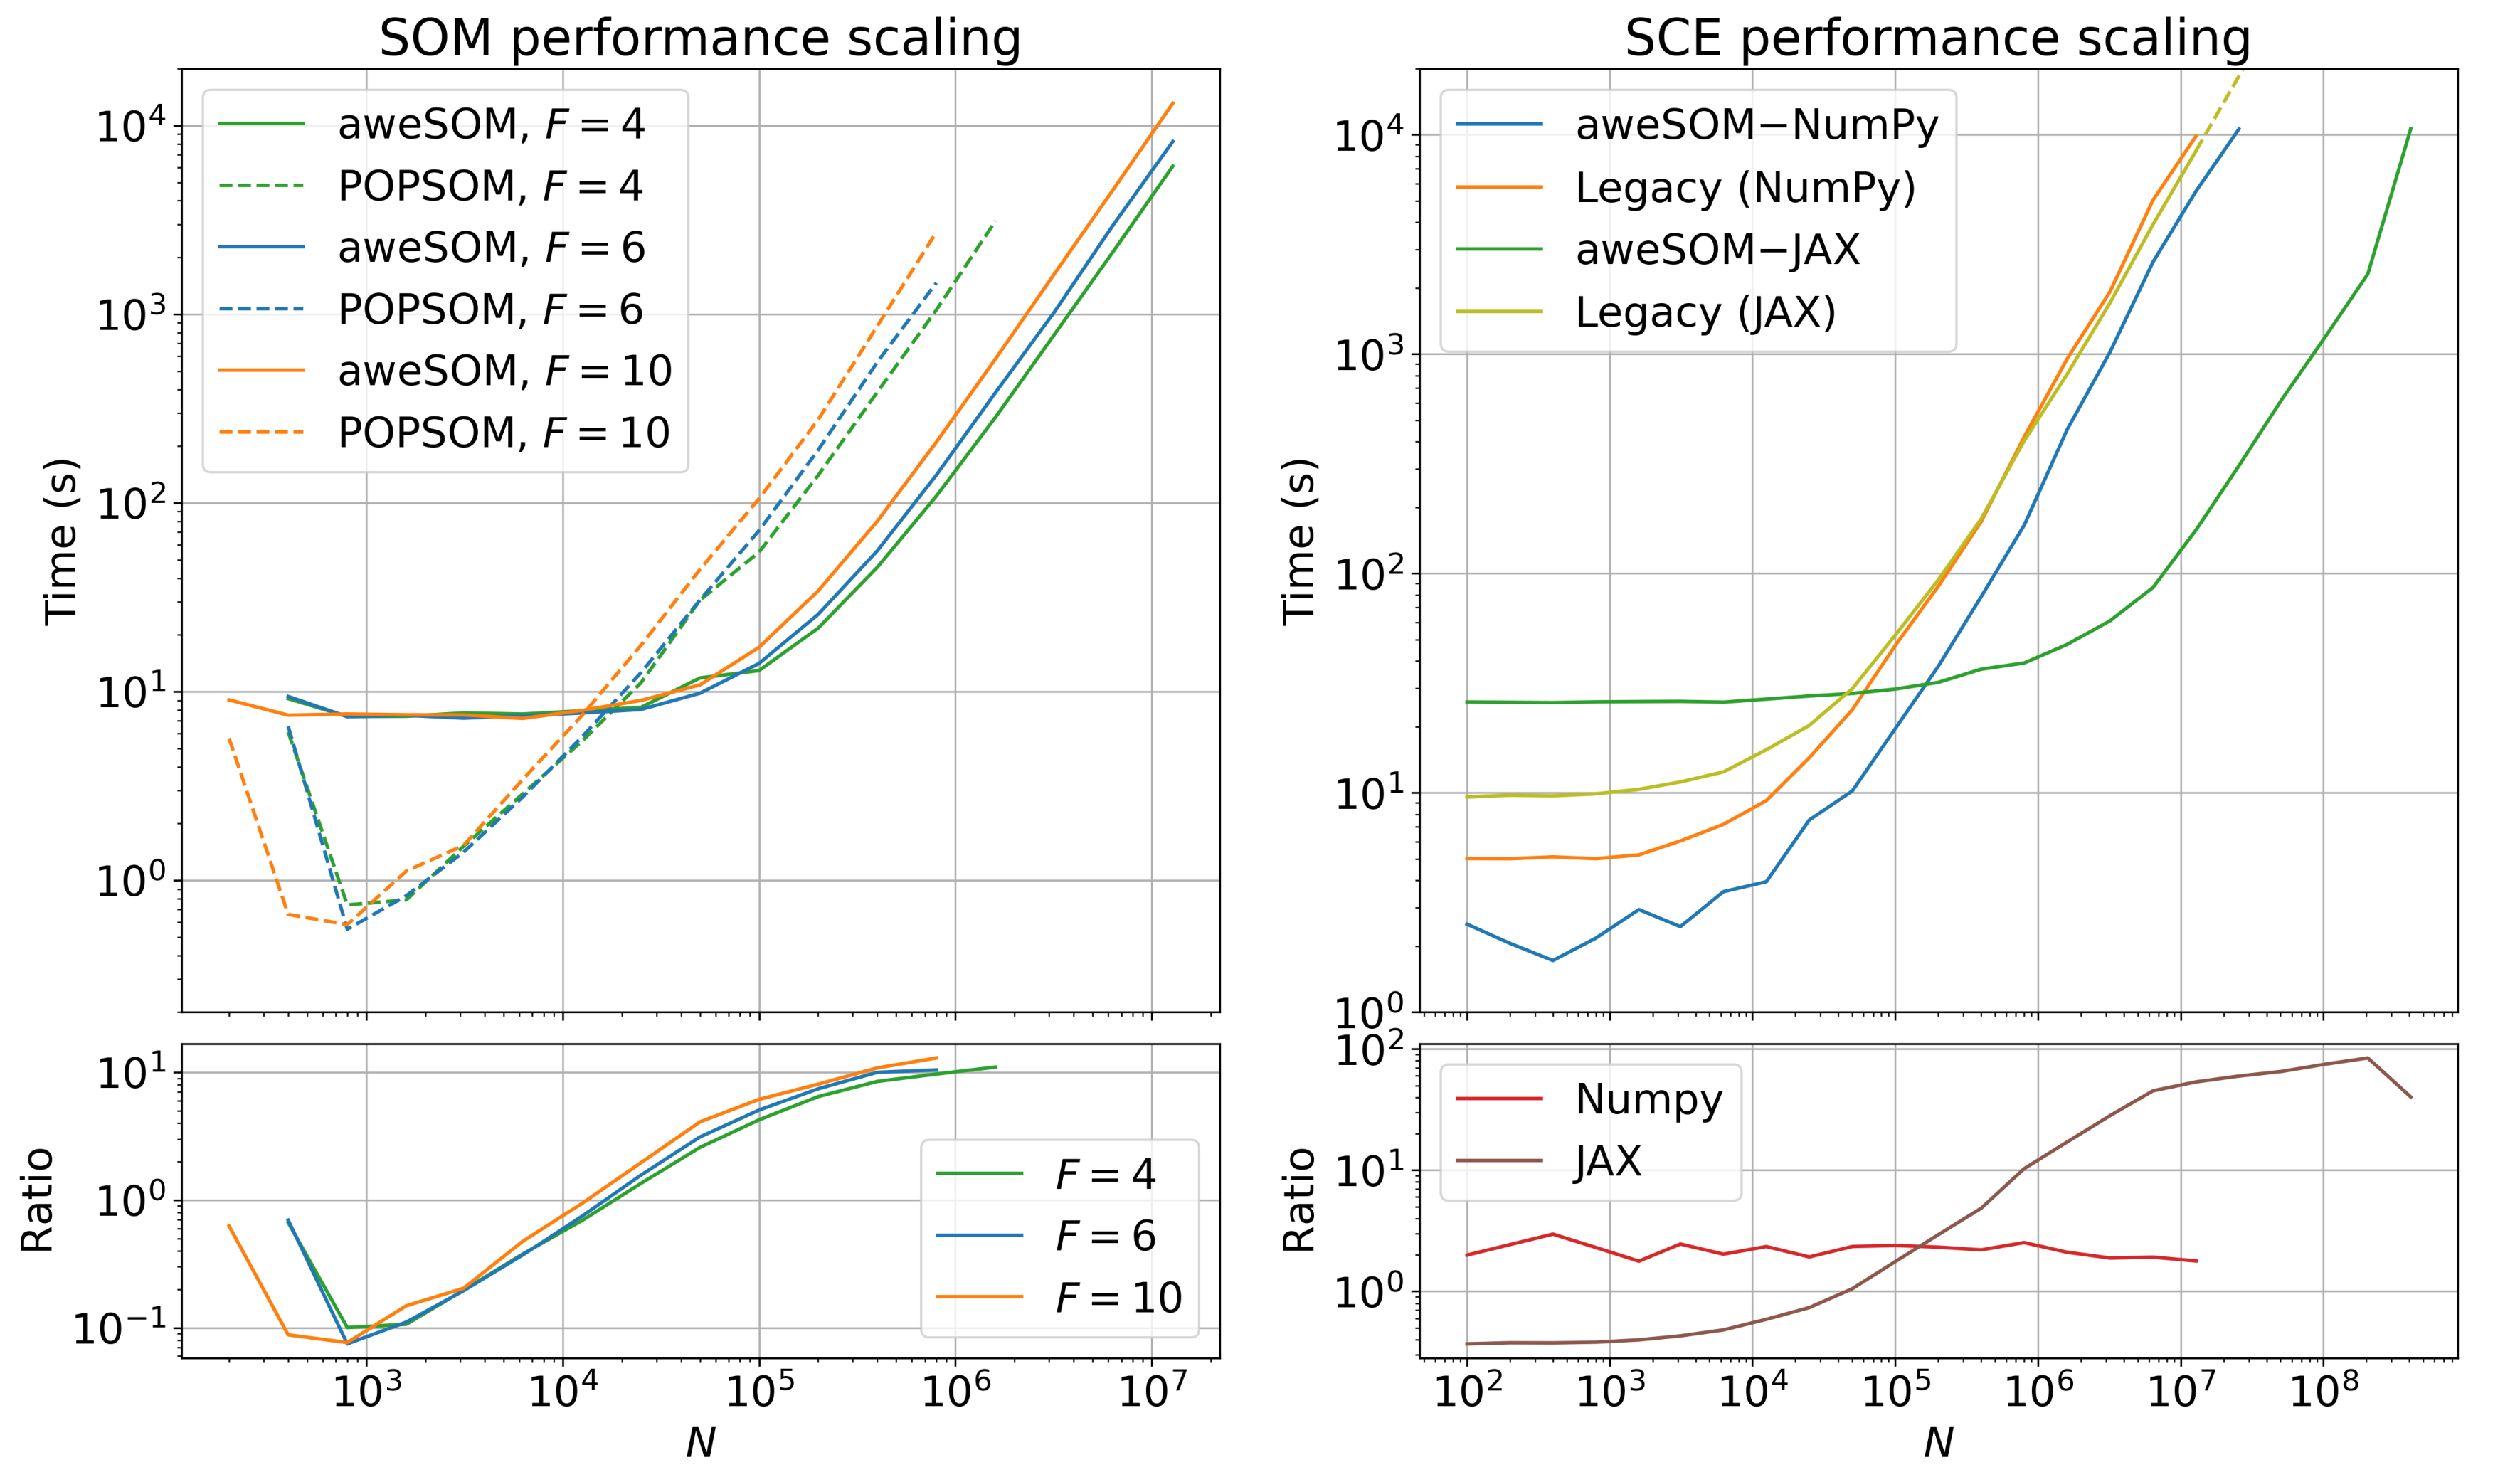
\includegraphics[width=\linewidth]{Plasma_img/joss_scaling.pdf}
    \caption{Performance scaling for \awesom\ vs.\ the legacy SOM (left) and SCE (right) implementation. The top panels show the time for each implementation to complete analysis of $N$ number of data points. On the right panel, the dotted line extending from the olive line shows linear extrapolations from the data in order to estimate the speedup. The bottom panels show the ratio between the time taken by the legacy code divided by the time taken by \awesom\@. In the SOM analysis, we consider a dataset with $F = 6$ and $F = 10$ dimensions. In the SCE analysis, we test the scaling of both a GPU-accelerated implementation (with \texttt{JAX}) and a CPU-only implementation (with \texttt{NumPy}).}
    \label{fig:sce_scaling}
\end{figure}


\section{Novel Characterization of Two Current Sheet Structures Enabled by \awesom}

\publicationdetails
{Ha et al.\ 2025, ApJL, 985, L31}
{Trung Ha\footnotemark[1]\footnotemark[2]\footnotemark[3], Joonas Nättilä\footnotemark[4]\footnotemark[2]\footnotemark[5], Jordy Davelaar\footnotemark[6]\footnotemark[2]\footnotemark[5]\footnotemark[7], and Lorenzo Sironi\footnotemark[8]\footnotemark[2]}
{The physics of turbulence in magnetized plasmas remains an unresolved problem. The most poorly understood aspect is intermittency---spatiotemporal fluctuations superimposed on the self-similar turbulent motions. We employ a novel machine learning analysis technique to segment turbulent flow structures into distinct clusters based on statistical similarities across multiple physical features. We apply this technique to kinetic simulations of decaying (freely evolving) and driven (forced) turbulence in a strongly magnetized pair-plasma environment, and find that the previously identified intermittent fluctuations consist of two distinct clusters: (i) current sheets, thin slabs of electric current between merging flux ropes; and (ii) double sheets, pairs of oppositely polarized current slabs, possibly generated by two nonlinearly interacting Alfvén-wave packets. The distinction is crucial for the construction of realistic turbulence subgrid models.}
{\footnotetext[1]{Department of Astronomy, University of Massachusetts Amherst, Amherst, MA 01003, USA}
\footnotetext[2]{Center for Computational Astrophysics, Flatiron Institute, 162 Fifth Avenue, New York, NY 10010, USA}
\footnotetext[3]{Department of Physics, University of North Texas, Denton, TX 76203, USA}
\footnotetext[4]{Department of Physics, University of Helsinki, P.O. Box 64, University of Helsinki, FI-00014, Finland}
\footnotetext[5]{Physics Department and Columbia Astrophysics Laboratory, Columbia University, 538 West 120th Street, New York, NY 10027, USA}
\footnotetext[6]{Department of Astrophysical Sciences, Peyton Hall, Princeton University, Princeton, NJ 08544, USA}
\footnotetext[7]{NASA Hubble Fellowship Program, Einstein Fellow}
\footnotetext[8]{Department of Astronomy, Columbia University, New York, NY 10027, USA}}
\setcounter{footnote}{0}

\subsection{Introduction} \label{sec:plasma-intro}

Turbulence is a seemingly chaotic mechanism occurring in fluids and plasmas \citep{davidson_turbulence_2015, biskamp_magnetohydrodynamic_2003}.
In practice, it enables a transfer of energy from a large scale $l_0$ onto smaller and smaller scales, $l_0 > l_1 > l_2 \ldots$, via the nonlinearities in the governing dynamical equations.
Classical theories of turbulence assume that this mechanism is volumetric and self-similar \citep{kolmogorov_local_1941}---that is, the shape of the turbulent eddies is identical on all scales $l < l_0$ within the inertial range.
On the other hand, experiments and numerical simulations have demonstrated that some structures in this flow become increasingly sparse in time and space as $l$ decreases \citep{she_universal_1994};
their distributions also become prominently non-Gaussian.
These spatio-temporal fluctuations of the turbulent flow can be broadly classified as \emph{intermittency}.

We focus on plasma turbulence where both the bulk velocities, $\mathbf{u}$, and the internal magnetic field fluctuations, $\mathbf{b}$, co-interact \citep{iroshnikov_turbulence_1964, kraichnan_inertial-range_1965, goldreich_toward_1995}.
Such plasma turbulence is ubiquitous in space physics and astrophysics, including, e.g., the solar corona \citep[e.g.,][]{parker_topological_1972, matthaeus_turbulence_1999}, interstellar medium \citep[e.g.,][]{larson_turbulence_1981, lithwick_compressible_2001}, and accretion flows around compact objects \citep[e.g.,][]{ripperda_magnetic_2020, nathanail_magnetic_2022}.
In these systems, intermittency plays a crucial role in controlling, e.g., (non-thermal) particle acceleration \citep[e.g.,][]{lemoine_particle_2023,nattila_radiative_2024}, cosmic ray transport \citep[e.g.,][]{fielding_plasmoid_2023,kempski_cosmic_2023}, and magnetic field amplification \citep[e.g.,][]{sironi_generation_2023,galishnikova_tearing_2022,beattie_magnetized_2024}.

The energy cascade by magnetized plasma turbulence is mainly controlled by the interaction between counter-propagating magnetic-shear-wave (Alfv\'en mode) packets \citep{goldreich_toward_1995}.
The nonlinear interaction between Alfv\'en waves is known to drive a secular energy transfer onto a higher-wavenumber Alfv\'en mode \citep{howes_alfven_2013,tenbarge_weak_2021}.
The generic picture has been confirmed in multiple numerical experiments \citep{nielson_alfven_2013,ripperda_weak_2021,nattila_heating_2022}.
What has remained poorly understood is the nature of the intermittency---i.e., deviations from this picture of co-interacting Alfven wave packets.
One manifestation of such deviation could, e.g., be the speculated dynamical alignment between $\mathbf{u}$ and $\mathbf{b}$ fields \citep{boldyrev_spectrum_2006}, or, more accurately, between the related Els\"asser fields, $\mathbf{z}_\pm = \mathbf{u} \pm \mathbf{b}$ \citep{mallet_refined_2015,chernoglazov_dynamic_2021}.
Another possibility is to interpret current sheets (and their interactions) as a manifestation of the intermittency \citep{zhou_spectrum_2023}.

We employ a theory-agnostic way of characterizing the intermittency in magnetically dominated plasma turbulence.
We study the nature of the intermittency in three-dimensional (3D) plasma turbulence using a combination of machine learning (ML) and computer vision techniques.
Namely, we identify structures consistent with \textit{current sheets} via a non-linear $N$-dimensional correlation with a CPU/GPU-accelerated implementation of self organizing maps \citep[SOM;][]{kohonen_self-organizing_1990}.
Then, we combine multiple realizations of the SOM model via a statistical ensemble learning framework to obtain statistically more reliable clustering solutions.
Intermittent structures in plasma turbulence have previously been identified and their statistics analyzed with the structure functions \citep{davis_intermittency_2024}, thresholding of current densities \citep{zhdankin_statistical_2013, kadowaki_mhd_2018}, Gaussian-fitting techniques \citep{greco_statistical_2009, chhiber_clustering_2020}, and, recently, ML-based segmentation \citep{serrano_scale_2025}.
Previous attempts at leveraging ML methods to detect current sheets include the $K$-means clustering and DBSCAN methods \citep{sisti_detecting_2021}, convolutional neural networks \citep{hu_identifying_2020}, and SOM \citep{bussov_maarja_segmentation_2021,kohne_unsupervised_2023, edmond_clustering_2024}.
These studies offer a promising outlook on the usability of novel computational methods to identify, in particular, current sheets in 2D simulations and in magnetospheric observations.
Our study is the first of its kind that applies such a technique to 3D simulations of highly-magnetized, relativistic plasma turbulence.

With this technique, we analyze the intermittent structures in the magnetically-dominated regime to find two distinct types of current sheets: single current sheets where magnetic structures of the same polarity are merging, and double current sheets where magnetic structures of opposite polarities are interacting.
Previous studies have mainly identified the single sheets \citep[e.g.,][]{zhdankin_statistical_2013,sisti_detecting_2021,davis_intermittency_2024} with some rare exceptions discussing the origin and formation of double-sheet structures \citep[e.g.,][]{howes_alfven_2013, howes_spatially_2018}.
Differentiation between the single and double sheets might have important consequences for understanding of the physics of dissipation in magnetized turbulence.

In Section~\ref{sec:simulation}, we describe the kinetic plasma simulation used in our analysis. We describe the ML method and its implementation in Section~\ref{sec:ml-method}. In Section~\ref{sec:result}, we report on the model's clustering results and on its implications in terms of the two distinct intermittent structures. In Section~\ref{sec:plasma-discussion}, we discuss our findings and implications for future research.

\subsection{Simulation} \label{sec:simulation}

\begin{figure}[htbp]
    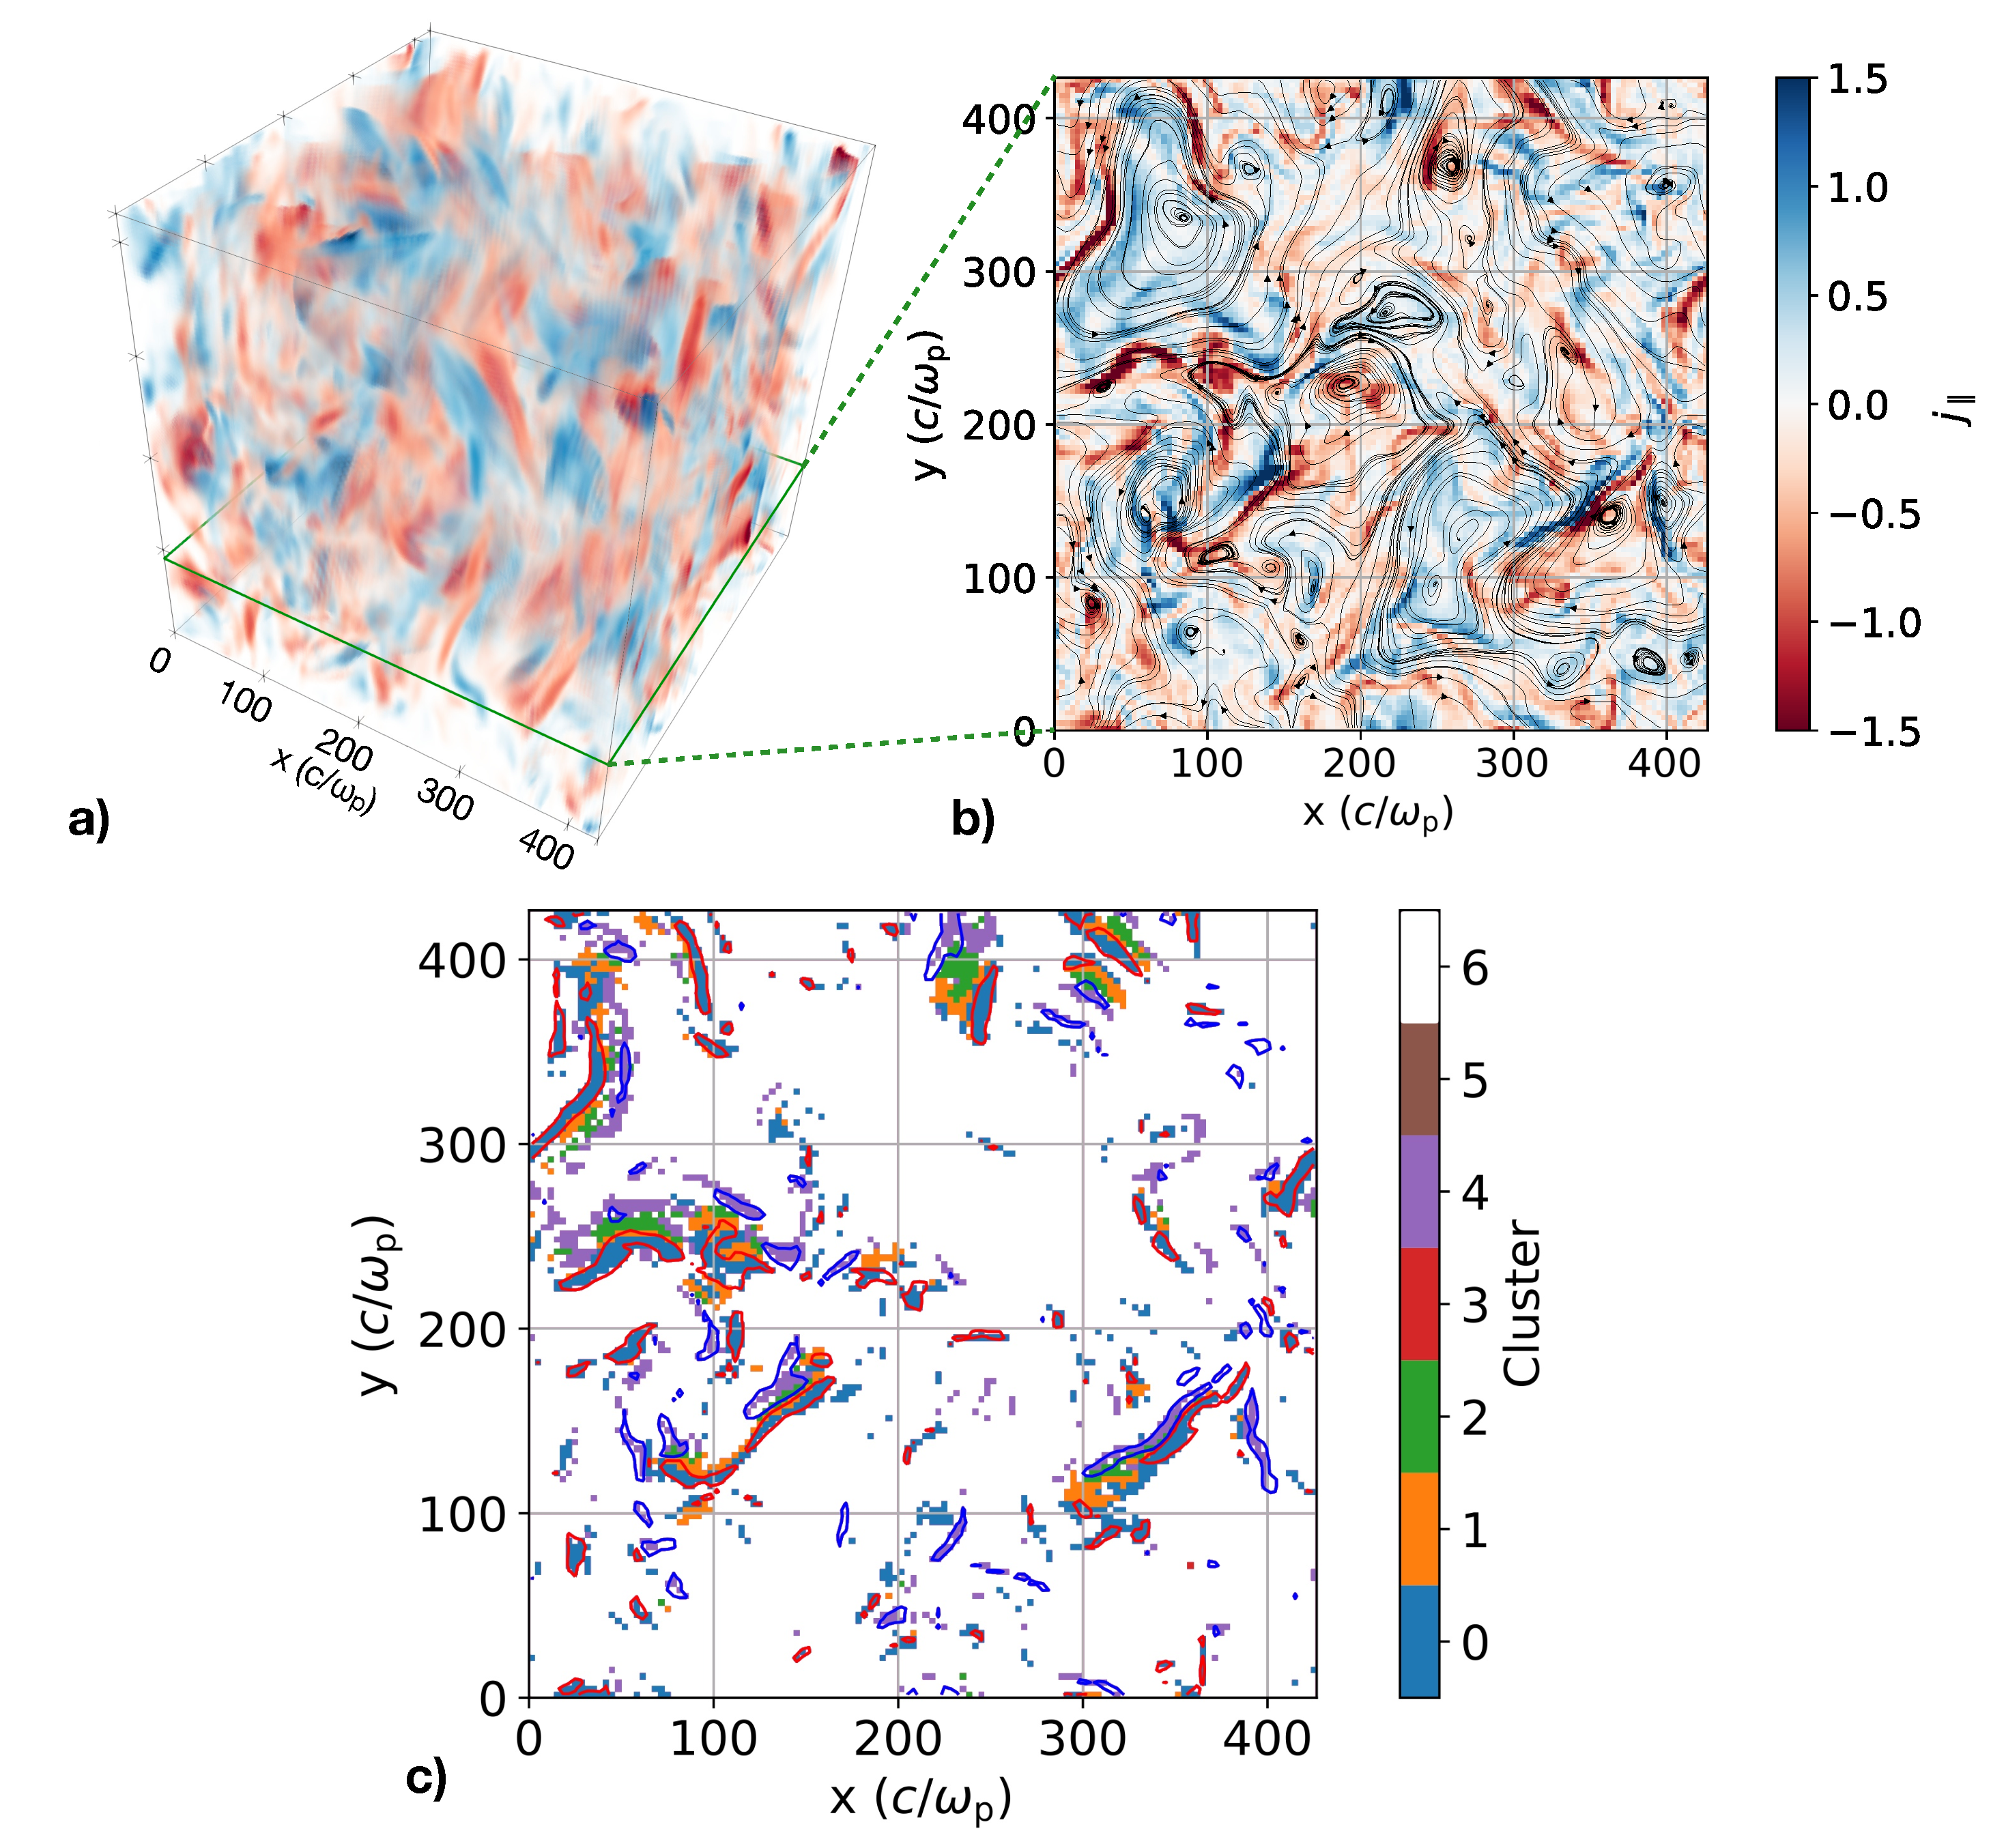
\includegraphics[width=\linewidth]{Plasma_img/fig1_key.pdf}
    \caption{Panel a): volume rendering of the projection of the current density onto the $\mathbf{B}$~field, \jpar. Panel b): $xy$-slice of \jpar~at $z=90\, c/\omega_{\rm p}$. Streamlines of the in-plane magnetic field \bperp\ are in the foreground. Panel c): fiducial SOM segmentation, color-coded by the cluster identified via \awesom\@. From observation and the radar charts in Figure~\ref{fig:cluster_umap}, green and orange correspond to regions in between double current sheets, purple to current sheets aligned with $\mathbf{B}$, and blue to current sheets anti-aligned with $\mathbf{B}$. Blue contours are regions where $j_{\parallel} > 2 \, j_{\parallel, \rm rms}$, and red contours are regions where $j_{\parallel} < -2 \, j_{\parallel, \rm rms}$.
    }
    \label{fig:jz}
\end{figure}

We analyze direct numerical simulations of 3D plasma turbulence.
We model the first-principle dynamics of the plasma with fully kinetic particle-in-cell (PIC) simulations \citep{birdsall_plasma_1991} using the open-source \texttt{runko} code \citep{nattila_runko_2022}.
Here, we report results from a domain characterized by a sudden excitation of turbulence, followed by the development of freely evolving (decaying) turbulence within the plasma.
Such a situation may be expected in the magnetic flaring events close to the accretion flows around black holes and/or neutron stars \citep[e.g.,][]{nattila_radiative_2024}.
Additionally, we have also verified that similar conclusions hold with continuously forced (driven) systems;
see SM~\ref{app:other-sims} for the analysis.

The technical details of the simulation are described in \citet{nattila_radiative_2021}.
Briefly, the simulation is a cubic box of size $L_{\rm sim} = 426\;c/\omega_{\rm p}$, covering 1280 grid cells per dimension.
The freely evolving system is initially in an unperturbed equilibrium state with neutral $e^\pm$-pair plasma, which is magnetized with a uniform external field $\mathbf{B_0} = B_0 \hat{\mathbf{z}}$.
We focus on the strongly magnetized domain where the magnetization parameter $\sigma \equiv B_0^2/4\pi n m_e c^2 \gtrsim 1$ (where $n$ is the plasma number density, $m_e$ is the electron rest mass, and $c$ is the speed of light).
We set $\sigma=10$.
We consider the simplest pair plasma composition to minimize the role of the kinetic effects, with 54 particles per $c^3/\omega_{\rm p}^3$ per species (two particles per cell per species).
The initial equilibrium is disturbed by exciting large-scale ($l_0 = L_{\rm sim}/4$) magnetic perturbations, $\delta \mathbf{B} \perp \mathbf{B_0}$ with a large amplitude $\delta B/B_0 \sim 1$.
The resulting plasma bulk motions are trans-relativistic, since $|\mathbf{u}| \approx v_A \approx c$, where $v_A \equiv c \sqrt{\sigma/(\sigma+1)}$ is the Alfv\'en velocity.
We follow the simulations until $t = 20\, l_{0}/c$ (where $l_0/c$ is the eddy-turnover time of the energy-carrying scale).
We store data snapshots (composed of $\mathbf{E}$, $\mathbf{B}$, and $\mathbf{J}$ fields) on a cadence of $\Delta t \approx 1 \, l_0/c$.
Numerically, each snapshot we analyze is a down-sampled rectangular cube composed of $L^3 = 128^{3} \approx 2 \times 10^6$ data points.
Figure~\ref{fig:jz}a shows a volume rendering of the projected current density along the $\mathbf{B}$ field, $j_{\parallel} \equiv \mathbf{J}\cdot\mathbf{B}/(Bn_0ec)$, together with a $xy$-slice plot of the same feature, over-plotted by streamlines of the in-plane magnetic field, $B_{\perp}$ in Figure~\ref{fig:jz}b.
We present the following results based on one representative snapshot of the simulation, taken at $t = 5\;l_0/c$, which exhibits a magnetic power spectrum  $\propto k_\perp^\alpha$ with a slope of $\alpha \approx -5/3$, where $k_\perp$ is the wavenumber perpendicular to the mean magnetic field.

\subsection{Clustering Analysis} \label{sec:ml-method}
We analyze the resulting large, multi-dimensional dataset with a ML technique called Self-Organizing Maps \citep[SOM;][]{kohonen_self-organizing_1990}.
SOM is a sophisticated classification method that can capture multi-dimensional correlations in the input data by exposing the topology of the (possibly nonlinear) manifolds being analyzed.
We employ the SOM algorithm specifically because it is a powerful, unsupervised method that does not require prior knowledge about the number of clusters (i.e., \textit{physical structures}). Furthermore, the resulting clustering of nodes in a SOM is easily interpretable.
We further enhance the robustness of the model by combining multiple SOM realizations through a statistically combined ensemble method \citep[SCE;][see also SM~\ref{app:sce}]{bussov_maarja_segmentation_2021}. SCE segmentation provides a statistically significant result by stacking SOM clusters of similar spatial distributions.
We provide a numerically fast implementation of the SOM and SCE methods as an open-source Python package called \awesom\footnote{\url{https://github.com/tvh0021/aweSOM/}} \citep{ha_awesom_2025}.
Specifically, the SOM implementation in \awesom\ is an optimized and parallelized version of the R package \texttt{POPSOM} \citep{hamel_vsom_2019}, providing a marked improvement in training time, and vastly superior projection (the mapping of cluster label from lattice space to real space) time, on the order of $\sim 20\text{--}50$ times faster.

\begin{figure}[htbp]
    \centering
    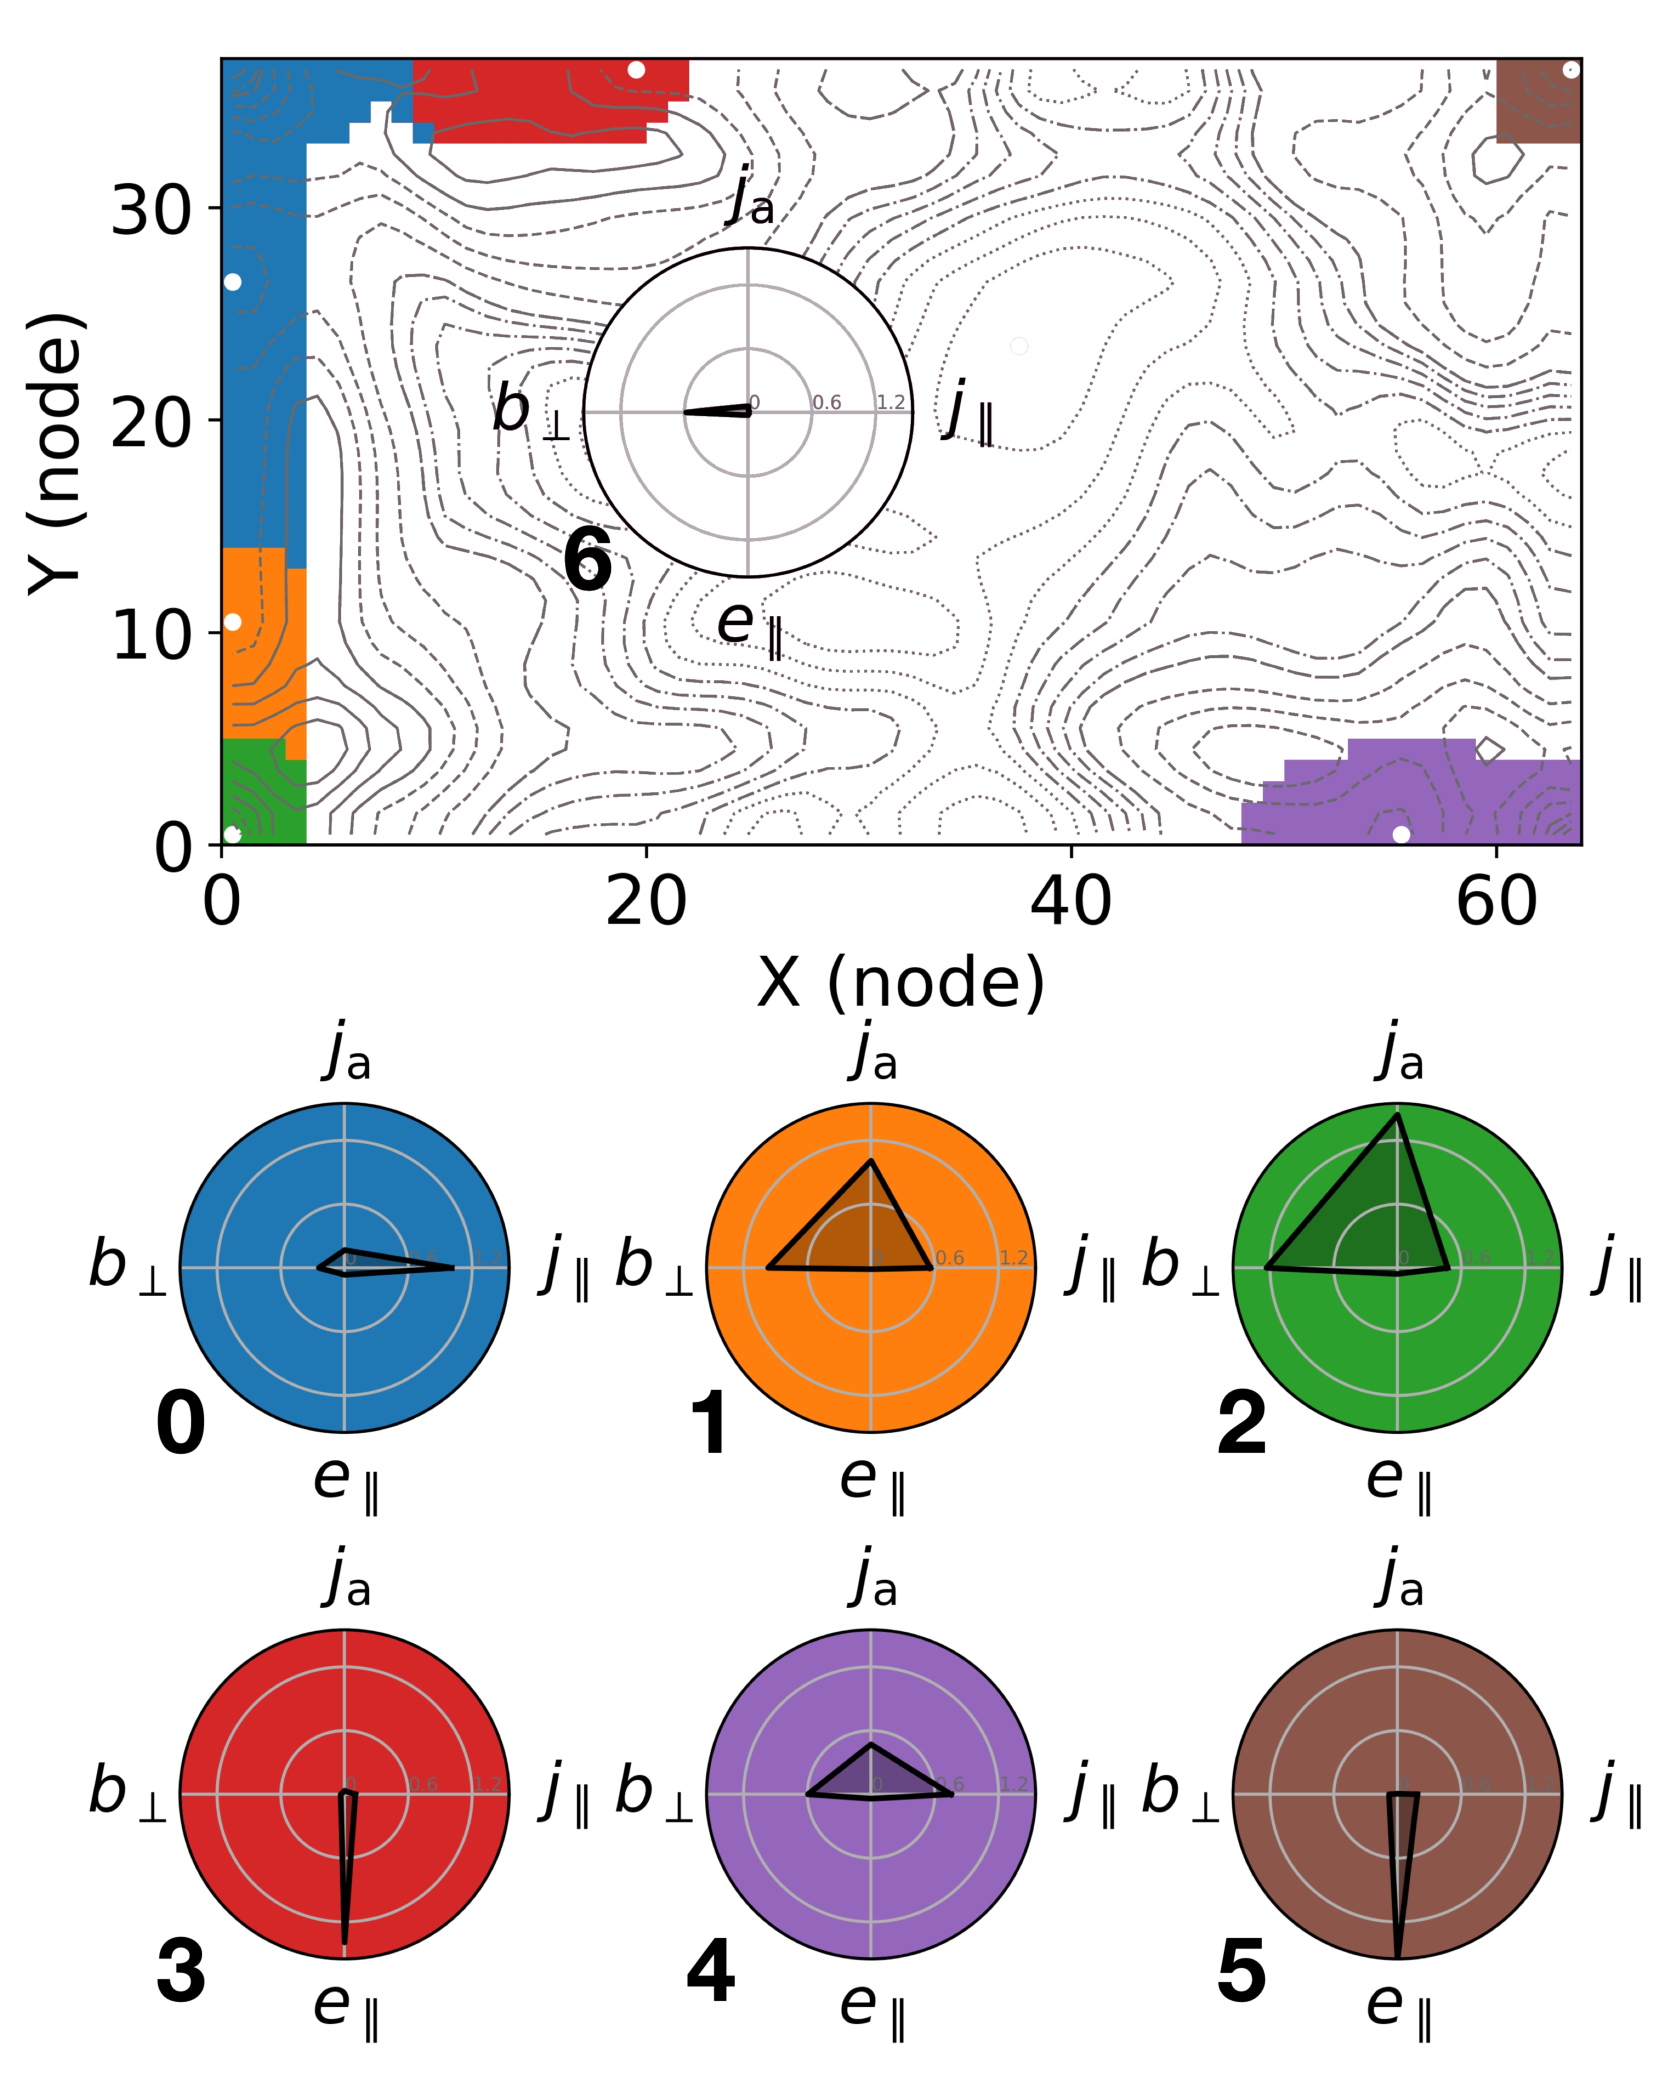
\includegraphics[width=0.9\columnwidth]{Plasma_img/fig2_key.pdf}
    \caption{Fiducial SOM representation of the plasma turbulence data with unified distance matrix (U-matrix).
    Each pixel in the map corresponds to a node in the lattice; the nodes are color-coded by their final cluster assignment.
    Cluster centroids are marked with white circles. In this example, seven clusters are identified.
    The map is overlaid with U-matrix isocontours, visualizing the lattice-space distance between the nodes. The style of the isocontours represents the value of the U-matrix in ascending order: dotted lines, dotted-dashed lines, dashed lines, and solid lines, respectively.
    The radar charts visualize the relative importance of each feature of the given cluster.
    }\label{fig:cluster_umap}
\end{figure}

For our fiducial analysis, we utilize four features to train the model:
\begin{enumerate}
    \item projection of the current along the magnetic field, $j_\parallel \equiv \mathbf{J}\cdot \mathbf{B}/(B n_0 e c)$,
    \item anti-symmetric convolution of the parallel current, $j_\mathrm{a} (\mathbf{x}) \equiv \int K_\mathrm{a}(\mathbf{y}) j_\parallel (\mathbf{x} - \mathbf{y}) \,\ud x \, \ud y$, where $K_\mathrm{a}$ is a two-dimensional anti-symmetric kernel (a discrete 1D counterpart is $\hat{K}_\mathrm{a}^{1\rm D} \equiv [-1, 0, 1]$),
    \item amplitude of the magnetic field in the $xy$-plane, $b_{\perp} \equiv b_{xy} \equiv (\mathbf{B} - \mathbf{B} \cdot \mathbf{\hat{z}})/B_0$,
    \item projection of the electric field along the magnetic field, $e_\parallel = \mathbf{E}\cdot\mathbf{B}/B_0$.
\end{enumerate}
Here, the anti-symmetric kernel $K_\mathrm{a}(r,\phi)$ (i.e., a matrix in our case) resembles the Heaviside-like function in a cylindrical coordinate system (as a function of $r$) and has, therefore, the property that
$K_\mathrm{a}(r < r_\mathrm{cut}, \phi \in [-\pi/2,\pi/2]) = 1$,
$K_\mathrm{a}(r < r_\mathrm{cut}, \phi \not\in [-\pi/2, \pi/2]) = -1$,
$K_\mathrm{a}(r > r_\mathrm{cut}, \phi) = 0$,
where $r_\mathrm{cut} = 3 c/\omega_{\rm p}$ is the kernel's extent, and $\phi$ is an angle against the direction set by $\nabla j_{\parallel}$.
In practice, if there is a location in the turbulent medium with doubly-peaked but oppositely directed current distributions with peaks of $-j_\mathrm{peak}$ and $+j_\mathrm{peak}$ next to each other in the $xy$-plane, then $j_{\rm a} \approx 2 j_\mathrm{peak}$ in between the peaks;
if the peaks are of same polarity, $+j_{\mathrm{peak},1}$ and $+j_{\mathrm{peak},2}$, then $j_{\rm a} \approx 0$.
Meanwhile, \jpar, \bperp, and \epar\ describe the magnitude of the current (which serves as a proxy for the current sheets), perpendicular magnetic field (a proxy for magnetic fluctuations), and non-linear electric field (a proxy for invalidity of ideal magnetohydrodynamics), respectively.

We normalize the input data before training such that each feature has a distribution with a mean $\mu = 0$\ and standard deviation $\sigma = 1.0$ (see SM~\ref{app:convergence} for a more detailed discussion).
With this approach, the four features are weighted equally by the model, while the outliers within each distribution are preserved, thus highlighting regions that experience strong intermittency.

Our fiducial SOM has a size of $64\times 37$ nodes in the lattice space.
The map is trained with an initial learning rate $\alpha_0 = 0.1$ for $N = L^3 \approx 2\times10^6$ steps.
We have found the reported map size to be the minimum viable option for adequately resolving the multi-dimensional feature space.
We use a map with an aspect ratio of $H = 37/64 \approx 0.6$.
The aspect ratio is selected to be close to the ratio of the first and second largest eigenvalues of the input data's principal components.
A detailed discussion of the technical parameters is given in SM~\ref{app:som}.
During our extensive tests (see SM~\ref{app:convergence} and \ref{app:distribution}), we found that the SOM lattice encompasses a surface in the 4D feature space, which is not easily translated to a physical connection.
For example, Figure~\ref{fig:lattice_triangle} shows projections of the lattice on pairs of features.
The nodes along $Y=0$ (the black line going from green to purple) span a wide range of values in \jasym, but does not show a similar behavior in any other feature.
At the same time, the nodes along $Y=36$ (the black line going from blue to brown) span both extremes in \epar.
The shorter lattice direction ($Y$), on the other hand, tends to separate the positive and negative data values;
physically, this can be interpreted as separating the directions aligned and anti-aligned with $\mathbf{B_0}$.

\subsection{Results} \label{sec:result}

\subsubsection{Fiducial SOM realization}

Figure~\ref{fig:cluster_umap} shows the unified distance matrix (U-matrix) of the trained SOM as isocontours.
The unified distance corresponds to the feature-space distance between adjacent nodes in the lattice.
For our fiducial case, the SOM detects seven clusters of distinct multi-dimensional correlations between the provided features.
We conclude that:
\begin{itemize}
\item Cluster 0 (blue in Figure~\ref{fig:cluster_umap}) shows a strong correlation with \jpar.
This is clearly seen when compared with a \jz~slice.
The cluster highlights regions with strong current density but where the direction is anti-aligned against $\mathbf{B}$.
\item Clusters 1 (orange) and 2 (green) have relatively strong \bperp~and \jasym, indicating the regions between double current sheets.
Because the y-axis of the U-matrix indicates the alignment with the direction of $\mathbf{B}$, cluster 1 is anti-aligned, while cluster 2 is aligned with $\mathbf{B}$.
\item Cluster 3 (red) and cluster 5 (brown) have exceptionally strong \epar.
These are regions where $\mathbf{E}$ strongly aligns with $\mathbf{B}$, indicating a breakdown of the (ideal) MHD approximation. Value-wise, cluster 3 indicates an anti-alignment with $\mathbf{B}$, while cluster 5 indicates an alignment with $\mathbf{B}$.
\item Cluster 4 (purple) is similar to cluster 0, but in these regions \jpar~align with $\textbf{B}$. There is a weak dependence on \bperp~and \jasym~that are more noticeable than in cluster 0, but this region is still representative of current sheets.
\item Lastly, cluster 6 (white) coincides with non-active background plasma regions and is thus of little physical interest to us here.
\end{itemize}

Altogether, clusters 0 and 4 are single current sheets in isolation, but when detected adjacent to clusters 1 and 2, they are components of double current sheets.
Taking a $xy$-slice as seen in Figure~\ref{fig:jz}b, we point to the structure at $x = 90\, c/\omega_{\rm p}$\ and $y = 400\, c/\omega_{\rm p}$\ as an example of a single current sheet, while at $x = 350\, c/\omega_{\rm p}$\ and $y = 150\, c/\omega_{\rm p}$\ a double current sheet is found.
The volume-filling fraction, $n_{\rm fill}$, of these clusters are (for cluster 0, 1, $\ldots$): $5.4\%$, $1.7\%$, $1.1\%$, $2.5\%$, $3.3\%$, $1.5\%$, $84.5\%$.
The regions with sheet-like structure contain a volume-filling fraction of $n_{\mathrm{fill,\, single+double}} \approx 11.5\%$ of the domain, which is in line with similar studies of strongly magnetized plasma turbulence \citep[e.g.,][]{tenbarge_current_2013,vega_electron-scale_2023}.
An additional statistical breakdown of each cluster is examined in SM~\ref{app:distribution}.

\subsubsection{Separating single and double current sheets}
\label{subsec:separate}


\begin{figure}[htbp]
    \centering
    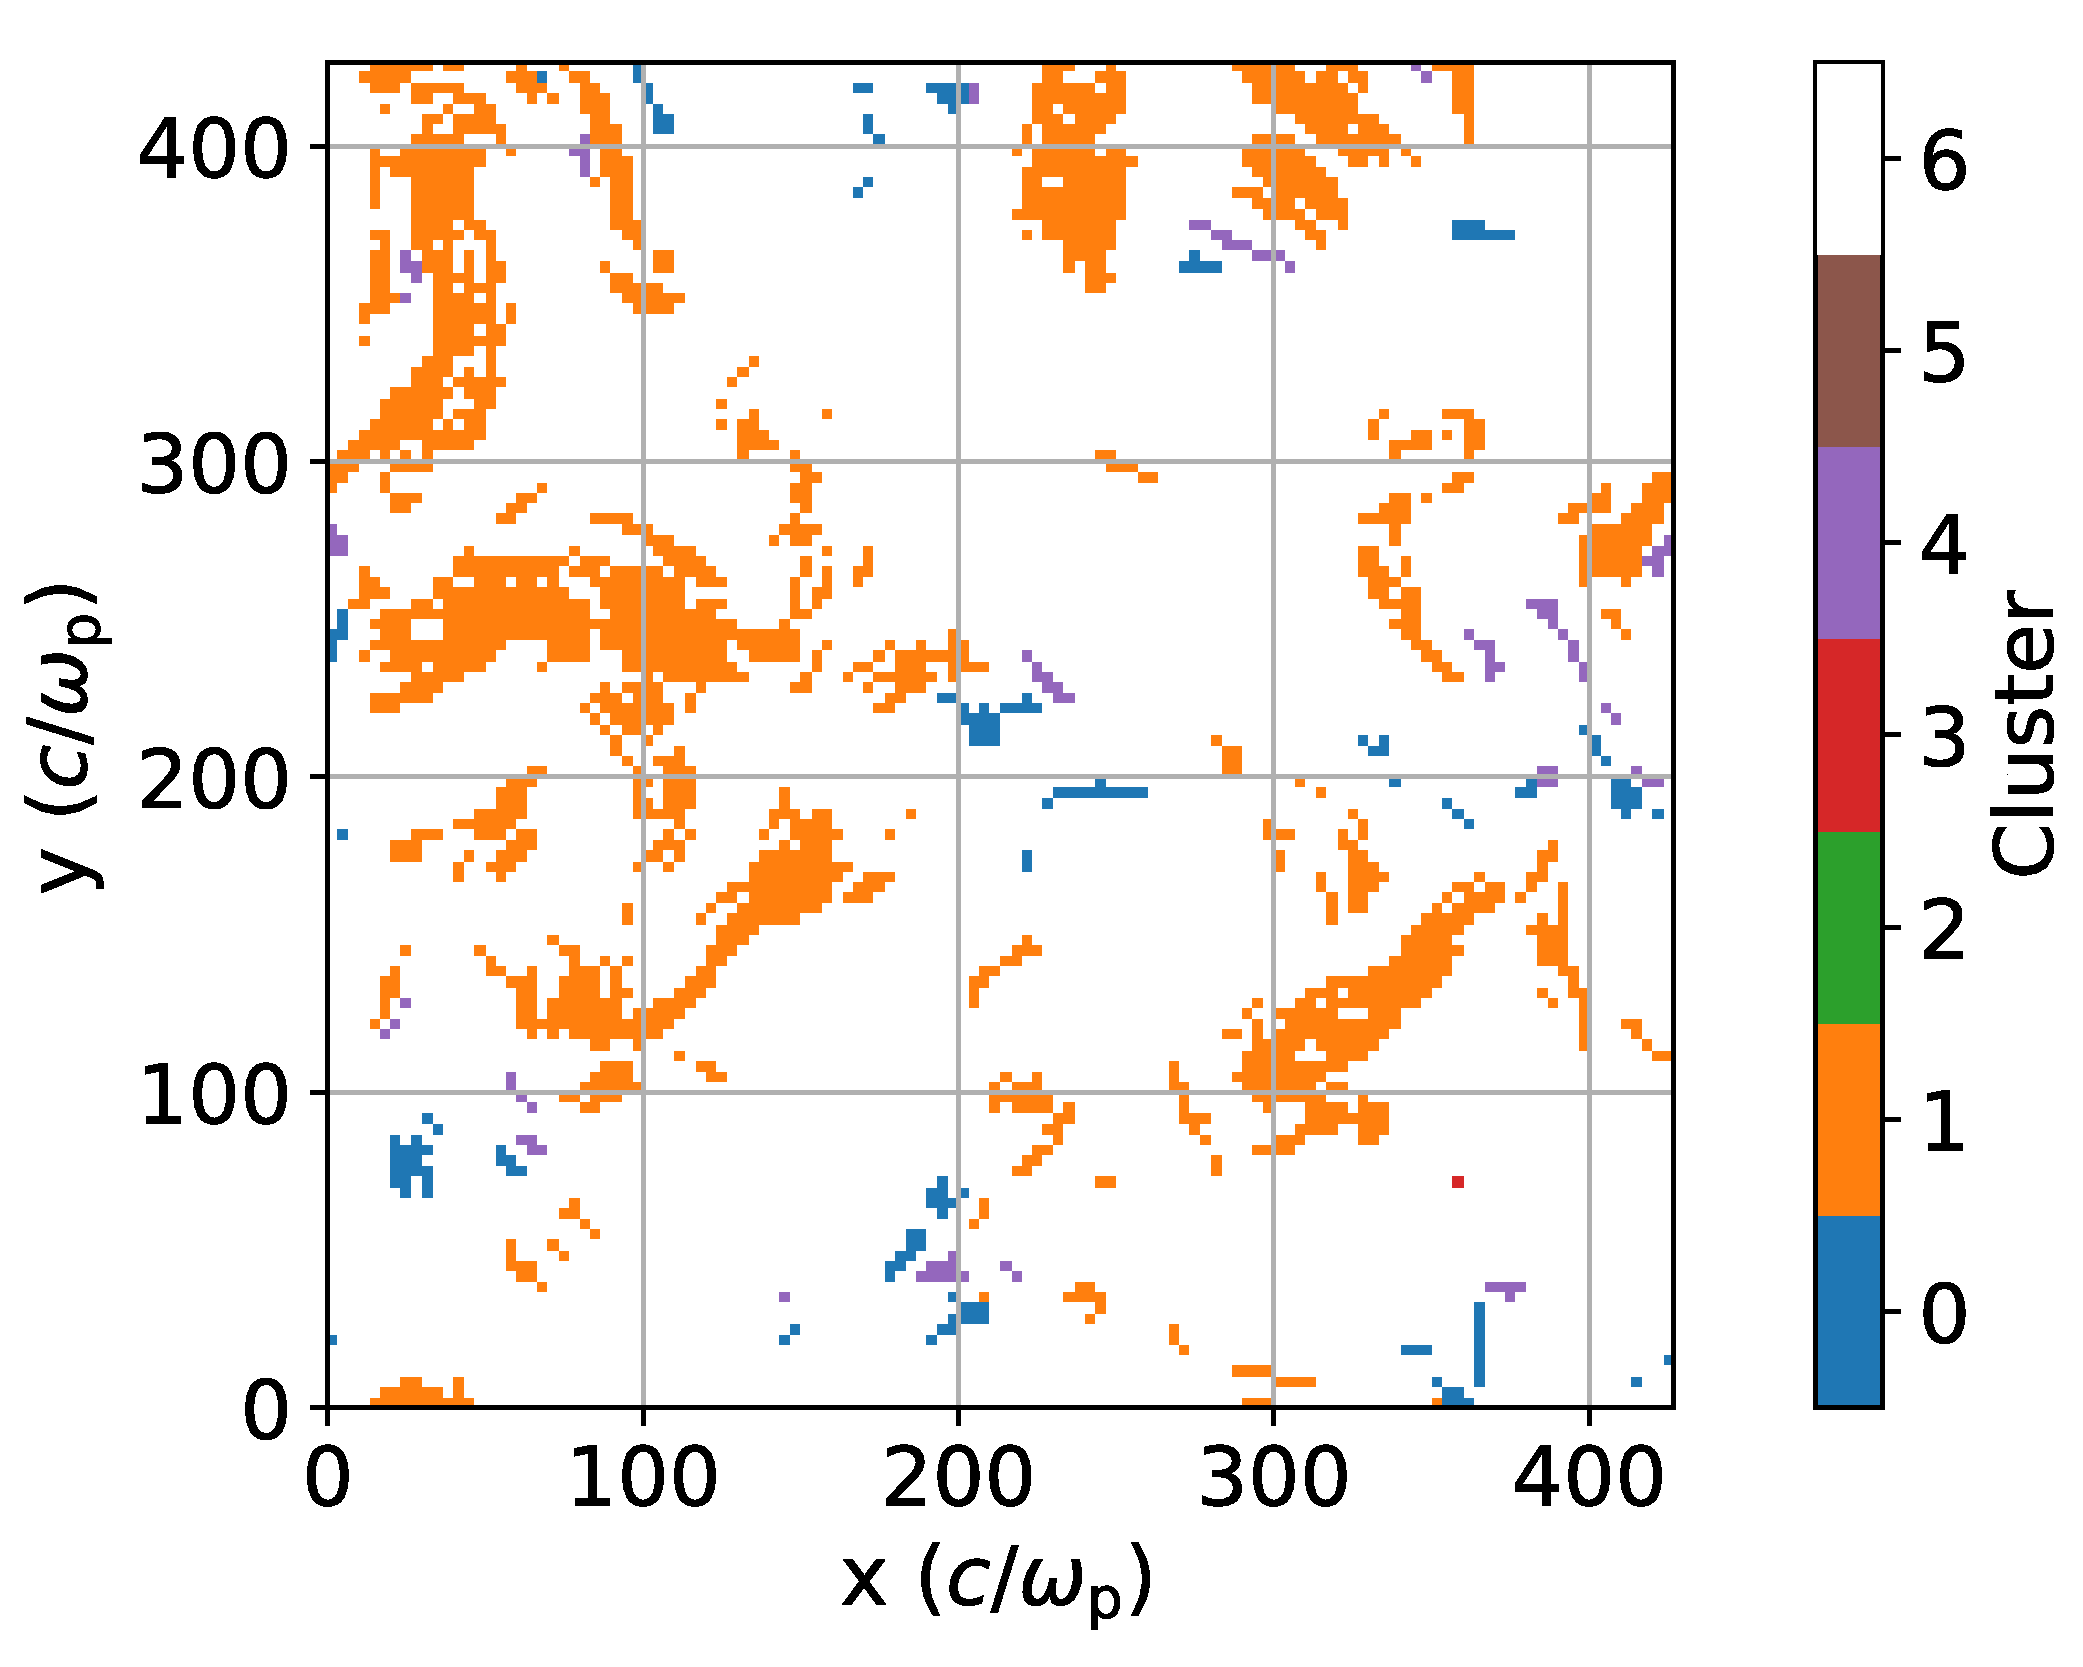
\includegraphics[width=\columnwidth]{Plasma_img/figmerged.pdf}
    \caption{Similar to panel c) of Figure~\ref{fig:jz}, but with adjacent clusters 0, 1, 2, and 4 merged into cluster 1. Cluster 1 denotes double current sheets, while clusters 4 and 0 denote single current sheets that align with \textbf{B} and anti-align with \textbf{B}, respectively.}
    \label{fig:merged_double}
\end{figure}

From the fiducial snapshot shown in Figure~\ref{fig:jz}c, we compute the volume-filling fraction of the single and double current sheets separately.
Since cluster 1 and 2 only occupy the spaces in between peaks of the double current sheets, we merge all continuous double sheets clumps with their adjacent single current sheets (cluster 0 and 4) into complete double current sheets.
The remaining clumps from cluster 0 and 4 that are not merged are true single current sheets.
Lastly, clumps identified as cluster 1 or 2 but are not found to be adjacent to both a $-j_{\rm peak}$ and a $+j_{\rm peak}$ are considered false detections, and are merged into the background cluster.

Figure~\ref{fig:merged_double} shows an $xy$-slice of the clustering result after merging, keeping the same color notations as in Figures \ref{fig:jz}c and \ref{fig:cluster_umap}.
Here, cluster 1 (orange) represents double current sheets; cluster 4 (purple) and cluster 0 (blue) are single current sheets that are aligned and anti-aligned with \textbf{B}, respectively; cluster 6 (white) is the background plasma; cluster 3 (red) and 5 (brown) are still locations of strong alignment between \textbf{E} and \textbf{B}.
Altogether, $n_{\rm fill,\, double} \approx 9.1\%$\ and $n_{\rm fill,\, single} \approx 1.5\%$.
When the system is allowed to reach steady state without continuous energy injection,
we find that most ``current sheet'' structures found are double current sheets. On the other hand, in continuously-driven turbulent environments, the relative fraction of single current sheets is more comparable to that of double current sheets ($n_{\rm fill,\, double} \approx 0.91\%$\ and $n_{\rm fill,\, single} \approx 0.46\%$ in our analysis; see SM~\ref{app:other-sims}).


\subsubsection{SCE result}

\begin{figure}[htbp]
    \centering
    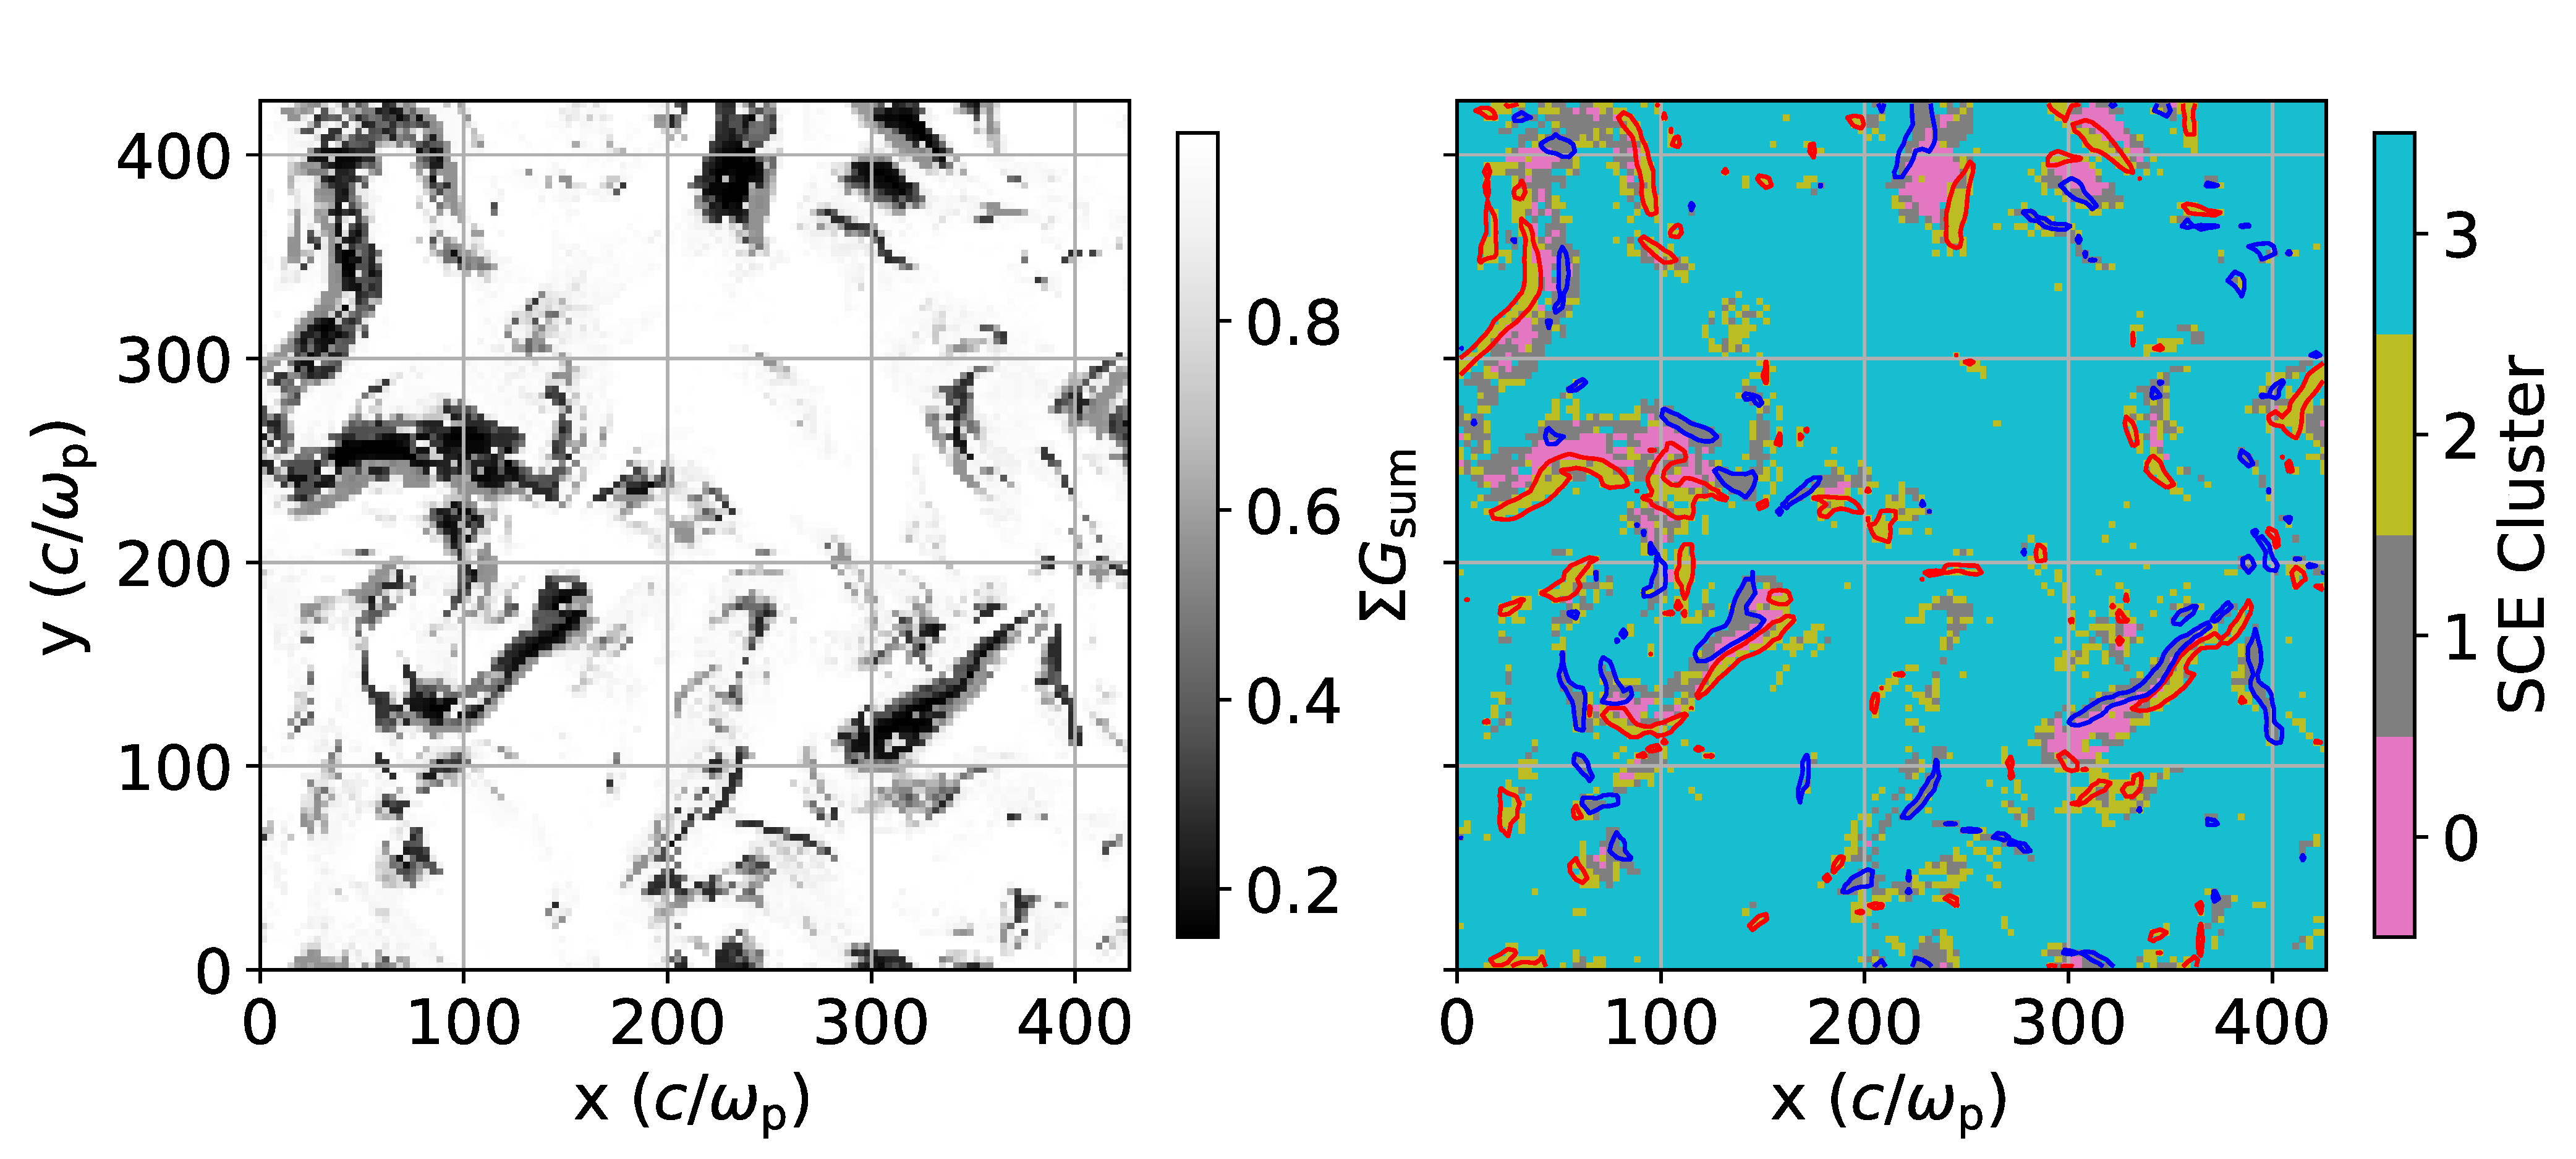
\includegraphics[width=\linewidth]{Plasma_img/sce_fig.pdf}
    \caption{SCE result obtained by combining the output of 36 SOM realizations.
    The left panel shows a $xy$-slice plot of $\Sigma G_{\rm sum}$ (signal strength) at $z = 90\, c/\omega_{\rm p}$.
    The right panel shows SCE clusters, obtained via making thresholds in the signal strength at 0.25, 0.5, and 0.8. Red and blue contours are the same as in Figure~\ref{fig:jz}c, and denote the regions where $|j_{\parallel}| > 2 \, j_{\parallel, \rm rms}$.
    Nominally, cluster 0 (pink) denotes double current sheets, cluster 1 (gray) denotes single current sheets aligned with $\mathbf{B}$, cluster 2 (olive) denotes single current sheets anti-aligned with $\mathbf{B}$, and cluster 3 (teal) denotes background plasma.}
    \label{fig:SCE_clusters}
\end{figure}

A key disadvantage of unsupervised ML methods compared to their supervised counterparts is the tendency of the final result to be highly dependent on the initial conditions \citep[e.g.,][]{attik_self-organizing_2005}.
We find very similar sets of final clusters when slightly varying the SOM hyperparameters ($N$, $H$, and $\alpha_0$). The results are also robust against the selected input features or turbulence parameters. However, as more features are added to the model, one would naturally expect to find more intrinsic clusters in the domain. Nevertheless, the clusters that specifically point to intermittency are always present.
These observations strongly suggest a universality of the obtained clusters by nature of a high-dimensional correlation between the most important features (\jpar, \jasym, \bperp, and \epar).

We quantitatively verify the robustness of these clustering results by conducting an SCE analysis on 36 different SOM realizations. The SCE clusters are derived by combining the strongest common features across the SOM realizations---features that are more universally present are indicated by stronger signals. Figure~\ref{fig:SCE_clusters} shows a $xy$-slice plot of the cumulative SCE \gsum\ values obtained via cluster-to-cluster comparison of all clusters $C$ in all \texttt{aweSOM} realizations $R$ (see SM~\ref{app:sce} for a more detailed definition of \gsum). The prominent clusters reveal four main structures: individual current sheets in olive and gray, double current sheets in pink, and the background plasma in teal.
We caution that, since the SCE analysis is run on the original SOM clustering results without post-processing, many of the individual sheets identified by the SCE algorithm are not of single type, but instead parts of the double-sheet structures if detected adjacent to cluster 0 (pink).
The more accurate statistical representation of the two types of intermittent structures is presented in Section~\ref{subsec:separate}.

\begin{figure}[htbp]
    \centering
    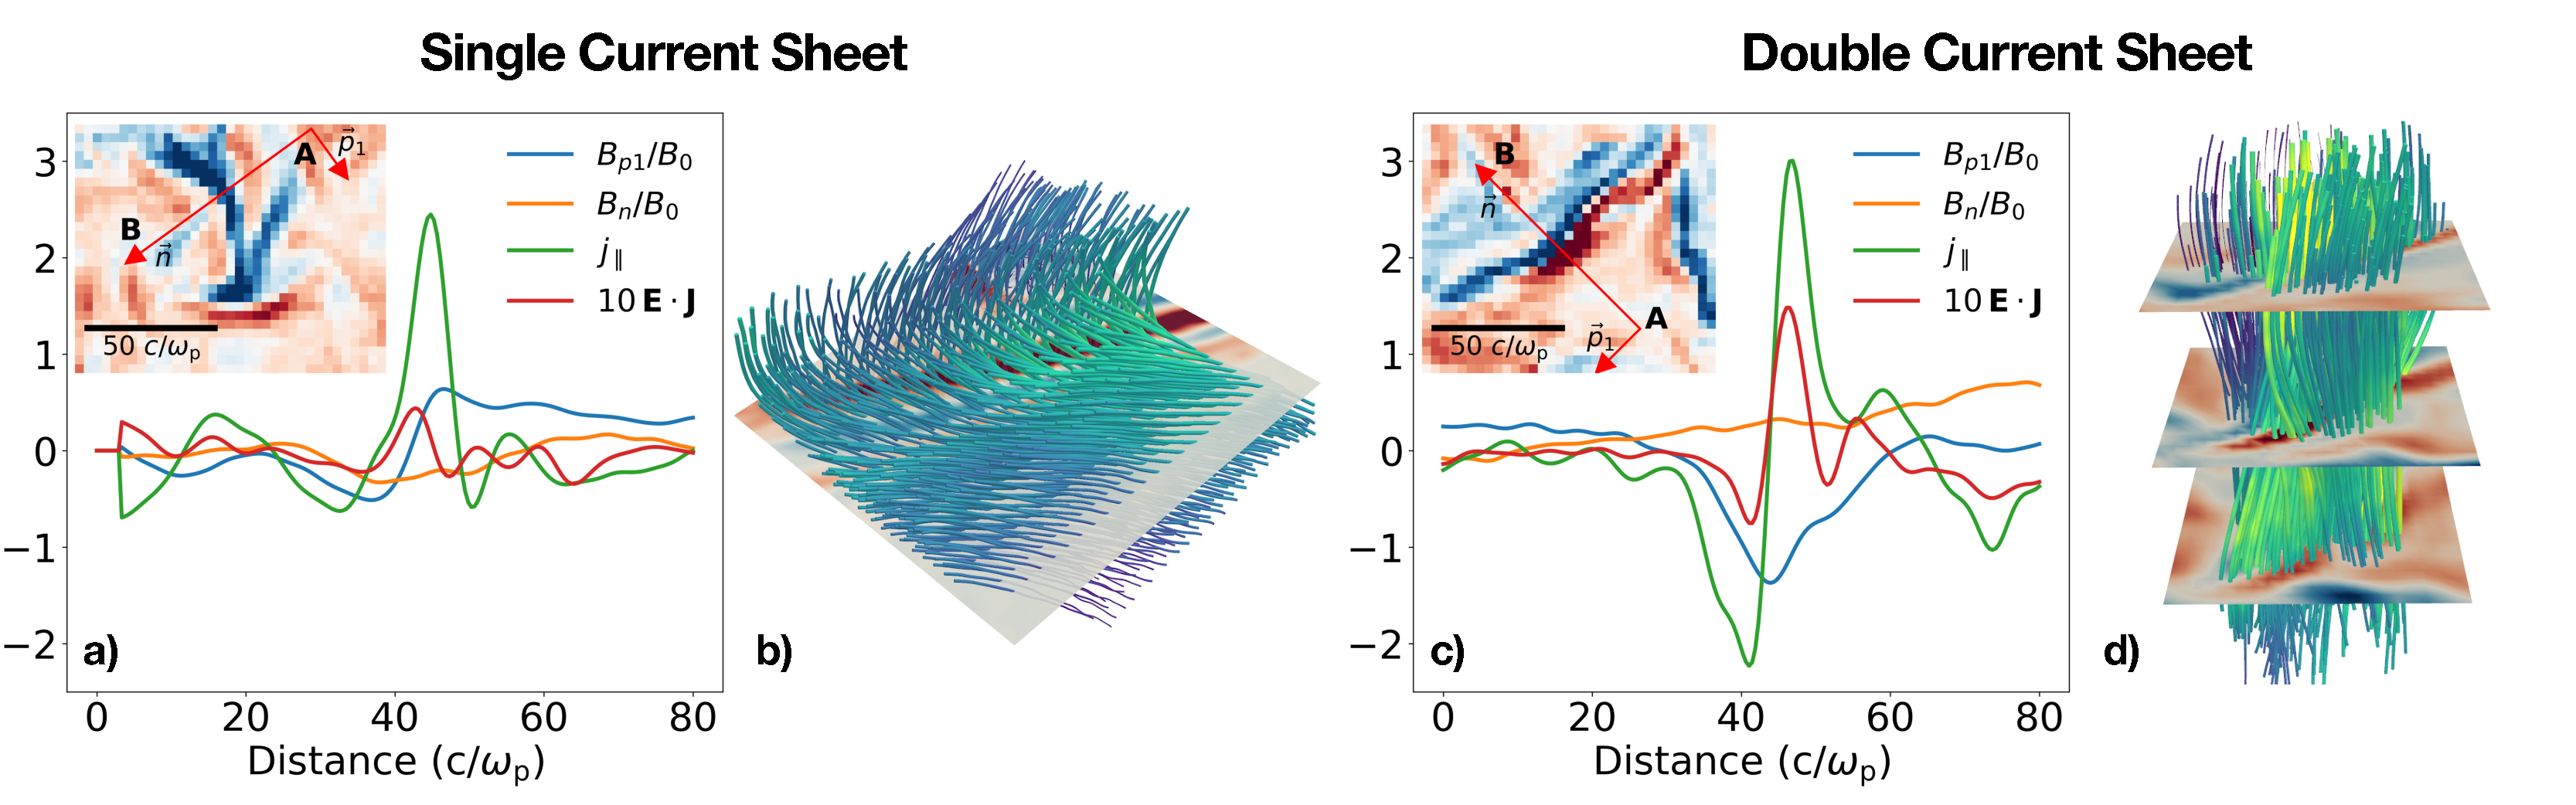
\includegraphics[width=\linewidth]{Plasma_img/fig3_key.pdf}
    \caption{Panel a) and c): line profiles of \jpar, $B_{n}/B_0$, $B_{p1}/B_0$, and $10\,\mathbf{E}\cdot\mathbf{J}$ along the line segment $\overline{AB}$. Each inset plot is a $xy$-slice of \jpar\ centered on the sheet of interest.
    Panel b) and d): volume rendering of $\mathbf{B}$~field lines, interlaced with $xy$-slices of \jz. On the left is an example of a single current sheet; on the right is an example of a double current sheet.
    }
    \label{fig:single_double}
\end{figure}

\subsubsection{Intermittency and current sheets}%
Interestingly, we find that some of the identified clusters are associated with spatio-temporal fluctuations in the simulation domain (clusters 0, 1, 2, and 4 in our fiducial analysis visualized in Figure~\ref{fig:jz}c and \ref{fig:cluster_umap} and cluster 0, 1, and 2 in Figure~\ref{fig:SCE_clusters}).
Physically, these clusters coincide with localized patches of intense electric current: \emph{current sheets}.
Because of this, we associate these clusters with MHD intermittency.
However, we always find two differing sheet-like structures in the flow.
This is in stark contrast with the previous analyses
\citep[e.g.,][]{chernoglazov_dynamic_2021,fielding_plasmoid_2023,davis_intermittency_2024}
that have assumed all current sheets to be of the same origin.

Figure~\ref{fig:single_double} shows an example of the two types of current sheets we regularly identify with the SOM analysis.
The inset plot in the top panels shows a $xy$-slice plot of \jpar, overplotted with a line segment $\overline{AB}$, which is approximately normal to the sheet(s).
We denote the direction along $\overline{AB}$ as $\mathbf{n}$, and the direction along $\mathbf{\hat{z}} \times \mathbf{n}$ as $\mathbf{p_1}$.
Then, we compute the line profile of \jpar, $B_{p_1}$, $B_n$, and $\mathbf{J} \cdot \mathbf{E}$~along $\overline{AB}$, and plot the profiles in panels a) and c).

The first type of cluster resembling intermittency is found in locations with large $j_\parallel$, small $j_\mathrm{a}$, and comparatively small $b_{xy}$ values (see clusters 0 and 4 in  Figure~\ref{fig:cluster_umap} and clusters 1 and 2 in Figure~\ref{fig:SCE_clusters}).
We call these structures \emph{single sheets}.
These single current sheets are classic exhibitions of intermittency via a reversal of magnetic polarity across the spatial domain.
Indeed, in Figure~\ref{fig:single_double}a, we find a relatively sharp peak in \jpar\ across a thickness of $\sim 5\,c/\omega_{\rm p}$.
A clear reversal in the magnetic polarity is also observed at this peak, where $B_{p_1}/B_0$ goes from $-0.5$ to $0.5$, and there is no definitive change in $B_n$.
In a realistic, turbulent flow, these structures are composed of magnetic field lines rapidly changing their orientation by about $90$ degrees, i.e., a classical magnetic reconnection setup in a moderate-to-strong guide field regime (see  Figure~\ref{fig:single_double}b).

The second type of cluster resembling intermittency is found in locations with large $j_\parallel$, large $j_\mathrm{a}$, as well as large $b_{xy}$ values (see cluster 1 and 2 in Figure~\ref{fig:cluster_umap}, and cluster 0 in Figure~\ref{fig:SCE_clusters}).
We call these structures \emph{double sheets} because they always come in pairs with oppositely directed currents.
Figure~\ref{fig:single_double}c shows the line profiles across one double sheet.
Importantly, rather than demonstrating a reversal in the magnetic polarity, there is a prominent peak in $B_{p_1}$ at the transition point between the sheets, indicating a sharp increase of the in-plane magnetic flux in the direction perpendicular to the sheet's surface normal.
In a realistic flow, these structures manifest as regions of the magnetic field with a separate, compressed core bundle oriented to a different direction than the neighboring field lines (see  Figure~\ref{fig:single_double}d).

\subsection{Discussion} \label{sec:plasma-discussion}
The formation of the single sheets is governed by the dynamics of the coherent structures in the turbulent flow \citep[e.g.,][]{zhou_spectrum_2023}.
First, we note that MHD turbulence tends to generate and sustain magnetic flux ropes (helical magnetic field structures with an electric current flowing along $\mathbf{B}$).
The dynamics between such structures follow from basic electrodynamics:
flux ropes with the same polarity attract;
opposite polarities repel each other.
Mergers of the same-polarity flux ropes form a reversal in the $\delta\mathbf{B} \perp \mathbf{B}_0$ magnetic field components;
such region naturally induces a spatio-temporal current sheet.
Such single sheets are prone to magnetic reconnection
\citep[e.g.,][]{priest_magnetic_2000,zweibel_magnetic_2009} and their lifetime is regulated by the tearing-instability \citep[e.g.,][]{comisso_interplay_2019} (or their environment).
They are well-known sites of plasma energization \citep{sironi_relativistic_2014, comisso_particle_2018}.

Importantly, our analysis also demonstrates that plasma turbulence tends to host a second type of current sheets, which has been largely overlooked so far.
These double sheets have been seen in previous numerical studies \citep[e.g.,][]{servidio_magnetic_2009, zhou_spectrum_2023} and observations of the Earth's magnetosphere \citep[e.g.,][]{ergun_observations_2009}; however, their statistics have not been analyzed nor has their importance been highlighted in the past.
The physical origin of the double current sheets remains uncertain.
Most likely, the double sheets arise from the nonlinear interactions between Alfv\'en wave packets \citep{howes_alfven_2013,howes_dynamical_2016,verniero_nonlinear_2018}.
In a freely-evolving relativistic pair plasma turbulence, we observe that the double current sheets are formed where magnetic structures of opposite polarities (i.e., rotational directions) are interacting.
However, even if their origin is not yet understood, their existence is important for future analysis of turbulence.
For example, it is not yet understood what scatters the energetic cosmic rays in the inter- and intra-galactic plasmas:
one hypothesis is the intermittent structures in the turbulence \citep{kempski_cosmic_2023,lemoine_particle_2023}.
A drastic difference in the shape of the (magnetic) structures can then lead to a significant difference in the scattering properties.
Lastly, the two intermittent structures also have differing dissipation profiles, which need to be explicitly accounted for in future turbulence sub-grid models that make assumptions about the local heating and particle acceleration.
For example, \citet{howes_spatially_2018} and \citet{nattila_heating_2022} found that Landau damping plays an important role in the energy dissipation of kinetic-Alfv\'en-wave turbulence.
Future studies on the stability of current sheets should also investigate the dissipation profile of these sheets, and whether they are analogous to the ``double tearing mode'' current sheets in the literature \citep[e.g.,][]{pritchett_linear_1980,baty_explosive_2013}.

\subsection{Supplemental Material}

\subsubsection{SOM segmentation method} \label{app:som}
SOM is an unsupervised ML technique that uses competitive learning for tasks like dimensionality reduction, clustering, and classification \citep{kohonen_self-organizing_1990}.
Fundamentally, a SOM is a 2D lattice of nodes that, through training, adapts to the intrinsic orientation of high-dimensional input data.

We develop a custom-made SOM implementation, \awesom\ \citep{ha_awesom_2025}.
This Python package employs the same technique as similar Python-based SOM implementations. Specifically, we base \awesom\ on \texttt{POPSOM}\footnote{\url{https://github.com/njali2001/popsom}}.
We introduce optimizations to improve analysis speed, enabling it to handle complex, high-dimensional physical data.
Below, we briefly describe \awesom's approach to learning the magnetized plasma turbulence.

First, we initialize a lattice of size $X\times Y \times F$, where $X$ and $Y$ are the number of nodes along each map direction, and $F$ denotes the number of features supplied to the model.
Before training, the initial weight value of each node, $\omega_0$, is randomly assigned, typically following a distribution representative of the input data.
The larger the lattice, the more details from the intrinsic data we can learn.
Kohonen \citep{kohonen_self-organizing_1990} advised using a lattice size of $N_{\rm node} = X \cdot Y = 5 \sqrt{N}$, where $N$ is the number of data points. We set $N_{\rm node} = \frac{5}{6} \sqrt{N \cdot F}$ such that the map both scales with the number of features in addition to the size of the data, but with a fraction of $\frac{1}{6}$ compensating for the map size quickly becoming too big to train when $N$ and $F$ are both large.

During each epoch, $t$, one input vector (a cell within the simulation domain) is randomly drawn.
Then, the Euclidean distances, $D_{\rm E}$, between this vector and all nodes in the lattice are calculated.
The node with the smallest distance is chosen as the best-matching unit (BMU)\@.
Then, the weight value of each node is updated:

\begin{equation}
    w_{i,j}(t) = w_{i,j}(t-1) - D_{\mathrm{E}|i,j} \cdot \gamma(t),
\end{equation}
where $i,j$ represent the node's location in the lattice, and $\gamma(t)$ is the neighborhood function:
\begin{equation}
    \gamma(t)= \begin{cases}
        \alpha(t) e^{\frac{-d_{\rm C}^2}{2(s(t)/3)^2}}, & \text{if $d_{\rm C} \leq s(t)$}\\
        0, & \text{if $d_{\rm C} > s(t)$}
    \end{cases},
\end{equation}
where $\alpha(t)$ is the learning rate at epoch $t$, $d_{\rm C}$ is the Chebyshev distance between the BMU and the node at $(i,j)$, and $s(t)$ is the neighborhood width at epoch $t$.

At the core of the SOM technique is the shrinking neighborhood.
Initially, $s_0 = \mathrm{max}(X,Y)$ such that earlier training steps adjust the weight values across the entire lattice.
As training progresses, $s$ gradually decreases until only a small number of nodes (or just the BMU) are updated each epoch.
In \awesom, the final neighborhood size is set to $s_{\rm f} = 8$.
This ensures that learning localizes to a specific region of the lattice without being overly restrictive, thereby preserving generalization.

After training, clustering is performed on the lattice based on the geometry of the U-matrix.
Cluster centroids are identified by finding local minima in the U-matrix.
A ``merging cost'' is then calculated by line integration between all pairs of centroids.
If the cost is below a threshold of 0.25 (with the cost between the two furthest centroids on the lattice normalized to one), the clusters are merged.
An example of the final clustering result on the lattice is shown in Figure~\ref{fig:cluster_umap}.

Lastly, the cells in the simulation are mapped to the nearest node in the lattice, each of which has been assigned a cluster label.
This label is then transferred to the corresponding input vector, resulting in visualization of the clustering in the input space.
An example of this mapping is shown in panel c) of Figure~\ref{fig:jz}.


\subsubsection{SOM convergence}\label{app:convergence}
We extensively test the convergence of the SOM clustering results by varying the key parameters before training: the number of training steps, $N$, the aspect ratio of the map, $H$, and the initial learning rate, $\alpha_0$.
Additionally, the choice of how to normalize the data before loading into \awesom, and how initial node values are assigned, can also contribute to the accuracy of the final clustering results.

We test the number of training steps required to reach convergence with $N$ from $10^4$~to $L^3$.
We find $N = 2\times10^5$~($\approx 10\% \; L^3$) to be on the lower bound for convergence, although higher $\alpha_0$~values (around 0.5) can allow convergence with fewer training steps.
Nevertheless, thanks to the relatively inexpensive cost of training a map, we choose $N=L^3=128^3$~for all cases.
Additional training by repeating the data does not appear to improve the results.

The initial learning rate $\alpha_0$ has a minimal impact on convergence, except when $N$ is small. During training, the learning rate is reduced at a constant rate such that the final learning rate $\alpha_{\rm f} = 10^{-3} \alpha_0$.
We use $\alpha_0 = 0.1$ for the fiducial realization but note that the U-matrices are qualitatively identical for $0.05 < \alpha_0 < 0.5$.

We also test the map's aspect ratio, $H$, by varying the ratio of vertical to horizontal nodes while keeping the total number constant.
Results are robust for $0.5 \lesssim H \leq 1$, and we use $H \sim 0.6$ in the fiducial realization, assuming a slight dominance of the data variance along one preferred direction.

We pre-process the data before training by normalization, testing three methods: \texttt{MinMaxScaler, StandardScaler} \citep{pedregosa_scikit-learn_2011}, and a custom normalization similar to \texttt{StandardScaler} but with a flexible range.
In the end, we found that the custom normalization with a mean $\mu = 0$~and standard deviation $\sigma = 1.0$~for each feature is optimal for map generation.

We also test different methods for initializing the map.
We choose the most general approach of drawing initial values from a uniform distribution with weights $-1 \leq w_0 \leq 1$.
Alternatively, the lattice can be initialized by drawing random observations (cells in the simulation domain) and assigning those values as initial weights \citep{ponmalai_self-organizing_2019}.
Ultimately, at $N = 128^3$, all initialization methods converge to similar final SOMs.

\subsubsection{SCE method} \label{app:sce}
\citet{bussov_maarja_segmentation_2021} discovered that their single SOM realizations were highly stochastic to small changes in the input parameters, raising concerns about the algorithm's stability.
To improve the robustness of these results, they developed an SCE method to stack multiple SOM realizations to obtain a single, markedly improved clustering result.
The mathematical details of the SCE framework are discussed in \citet{bussov_maarja_segmentation_2021}.
Below, we summarize the key concepts of SCE and how we integrate it into \awesom.

SCE involves a series of steps that stacks $n$~number of SOM realizations. For each cluster $C$ in a SOM realization $R$, its spatial distribution is compared with all other clusters $C'$ in $R' \neq R$ to obtain a goodness-of-fit index $g$. Then, each cluster $C$ is associated with a sum of goodness-of-fit (i.e., ``quality index''):
\begin{equation}
    G_{\rm sum} = \sum_{C_i' \in R'} g_i.
\end{equation}
Once all \gsum\ values are obtained, they are ranked in descending order, and groups of similar \gsum\ values are combined to form SCE clusters.
This approach works because clusters with similar spatial distributions tend to have similar \gsum\ values \citep[see Figure 6 of][]{bussov_maarja_segmentation_2021}. In practice, we do not rank the \gsum\ values, but instead sum this index point-by-point to obtain a general ``signal strength'' of each cell in the simulation.

Single \awesom\ realizations of the 3D simulation are found to be robust when introducing small changes in the initial conditions (see the previous subsection).
We independently confirm this robustness using SCE\@.
Since this stacking process involves extensive tensor multiplications, we utilize GPU-accelerated computation with \texttt{JAX} \citep{bradbury_jax_2018} and integrate this capability with \awesom\@.
As a result, \awesom\ can perform SCE analysis on high-resolution ($N \gtrsim 1000^3$) 3D simulations using one GPU (we ran the SCE analysis on an NVIDIA V-100 with 32 GB of VRAM)\@.
The final SCE clustering result is shown in Figure~\ref{fig:SCE_clusters} and discussed in more detail in the next section.

\subsubsection{SCE clustering result} \label{app:sce-result}
We perform SCE analysis on a set of 36 SOM realizations, exploring a parameter space of $10^6 \leq N \leq 4 \times 10^6$, $0.4 \leq H \leq 1$, and $0.1 \leq \alpha_0 \leq 0.4$.
We identify four statistically significant clusters. Figure~\ref{fig:SCE_clusters} highlights the prominence of each cluster as a cumulative sum of the number of pairs across the different SOM realizations that are detected at the same location.
In the left panel, each pixel is color-coded based on its normalized $\Sigma$\gsum\ (signal strength).
It is immediately clear that the background plasma has the highest signal strength ($\Sigma G_{\rm sum} > 0.8$) due to its high volume-filling fraction.
The intermittent structures are found at lower signal strengths, with the single current sheets at the intermediate level ($0.25 \lesssim \Sigma G_{\rm sum} \lesssim 0.8$), and the double current sheets at the lowest signal strengths ($\Sigma G_{\rm sum} \lesssim 0.25$).
After setting three thresholds at $\Sigma$\gsum\ at 0.25, 0.5, and 0.8, we can point to cluster 0 as the double current sheets, cluster 1 (2) as the individual sheets where \jpar\ aligns (anti-aligns) with $\mathbf{B}$, and cluster 3 as the background plasma.
The robustness of the reported clusters strongly indicates that the required input properties are universal and set by the physics of the turbulence.

\subsubsection{Statistical Distributions of SOM clusters} \label{app:distribution}

\begin{figure}[htbp]
    \centering
    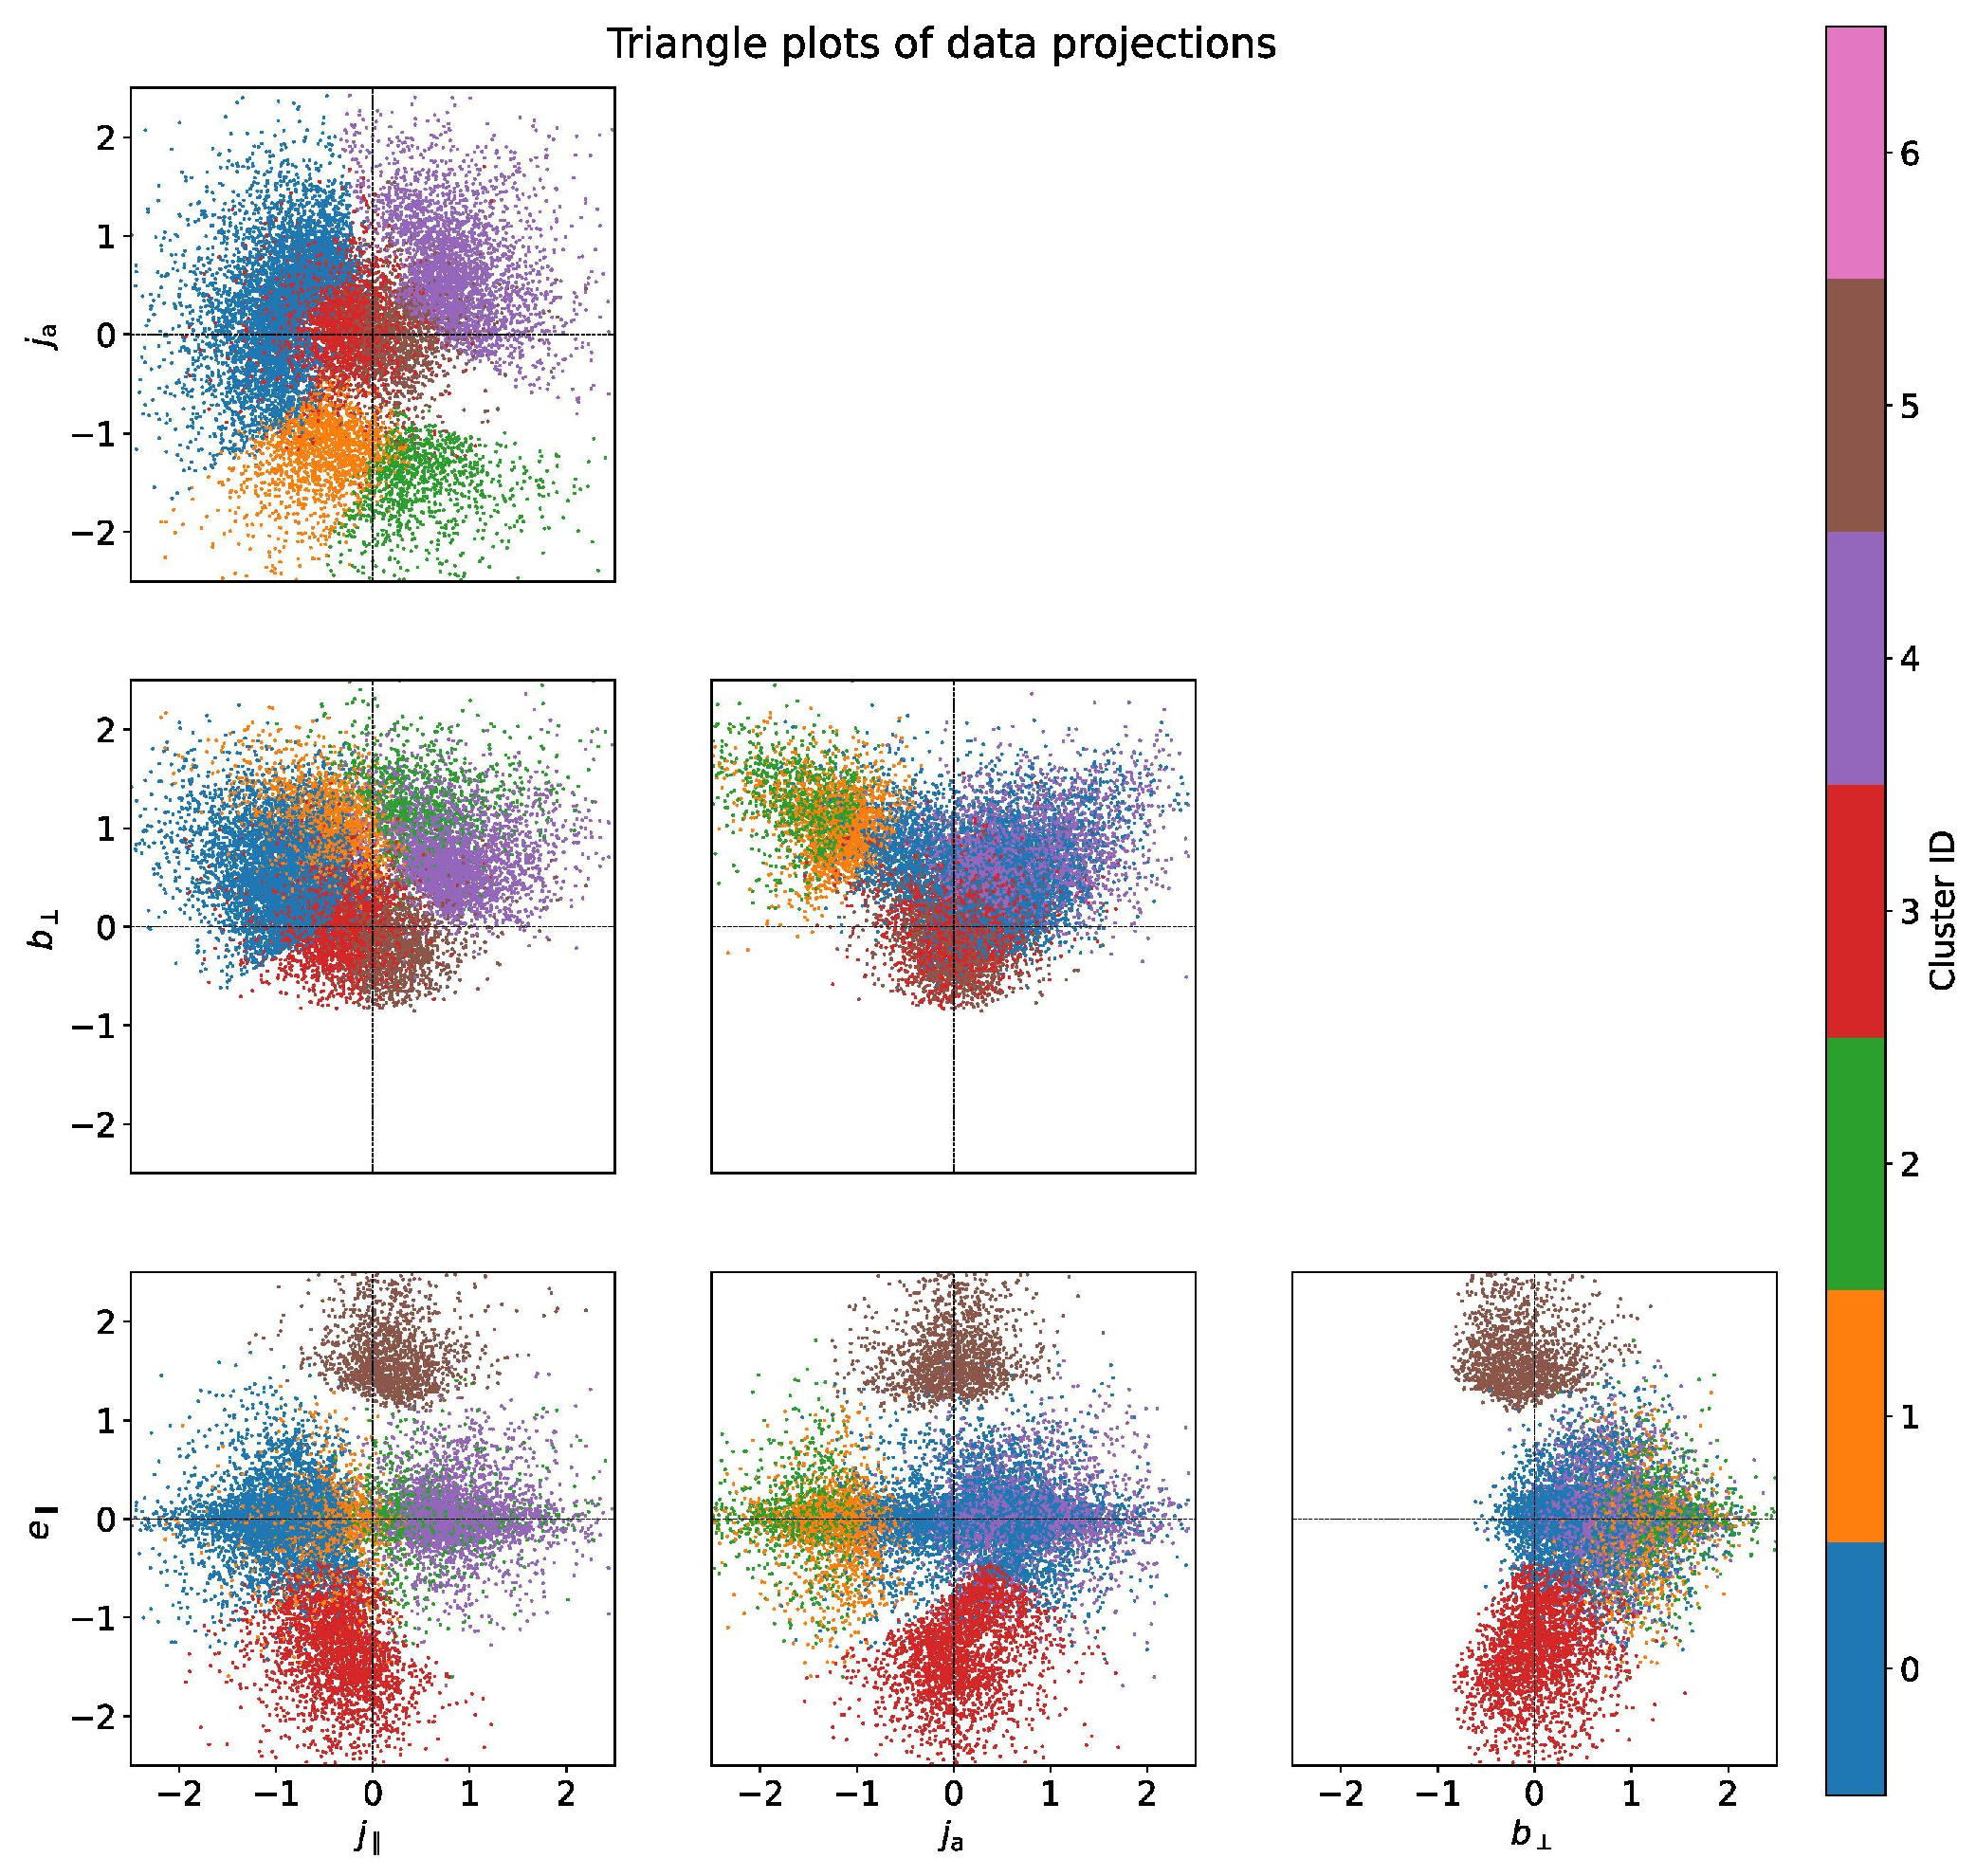
\includegraphics[width=0.9\linewidth]{Plasma_img/data_triangle.pdf}
    \caption{Feature-to-feature scatter plots of SOM clusters from Figure~\ref{fig:cluster_umap}. For clarity, cluster 6 has been excluded, and a random sample of $10^5$ points ($\sim 5\% \,L^3$) is drawn for each plot. Each data point is color-coded by its assigned cluster label.}
    \label{fig:triangle}
\end{figure}

\begin{figure}[htbp]
    \centering
    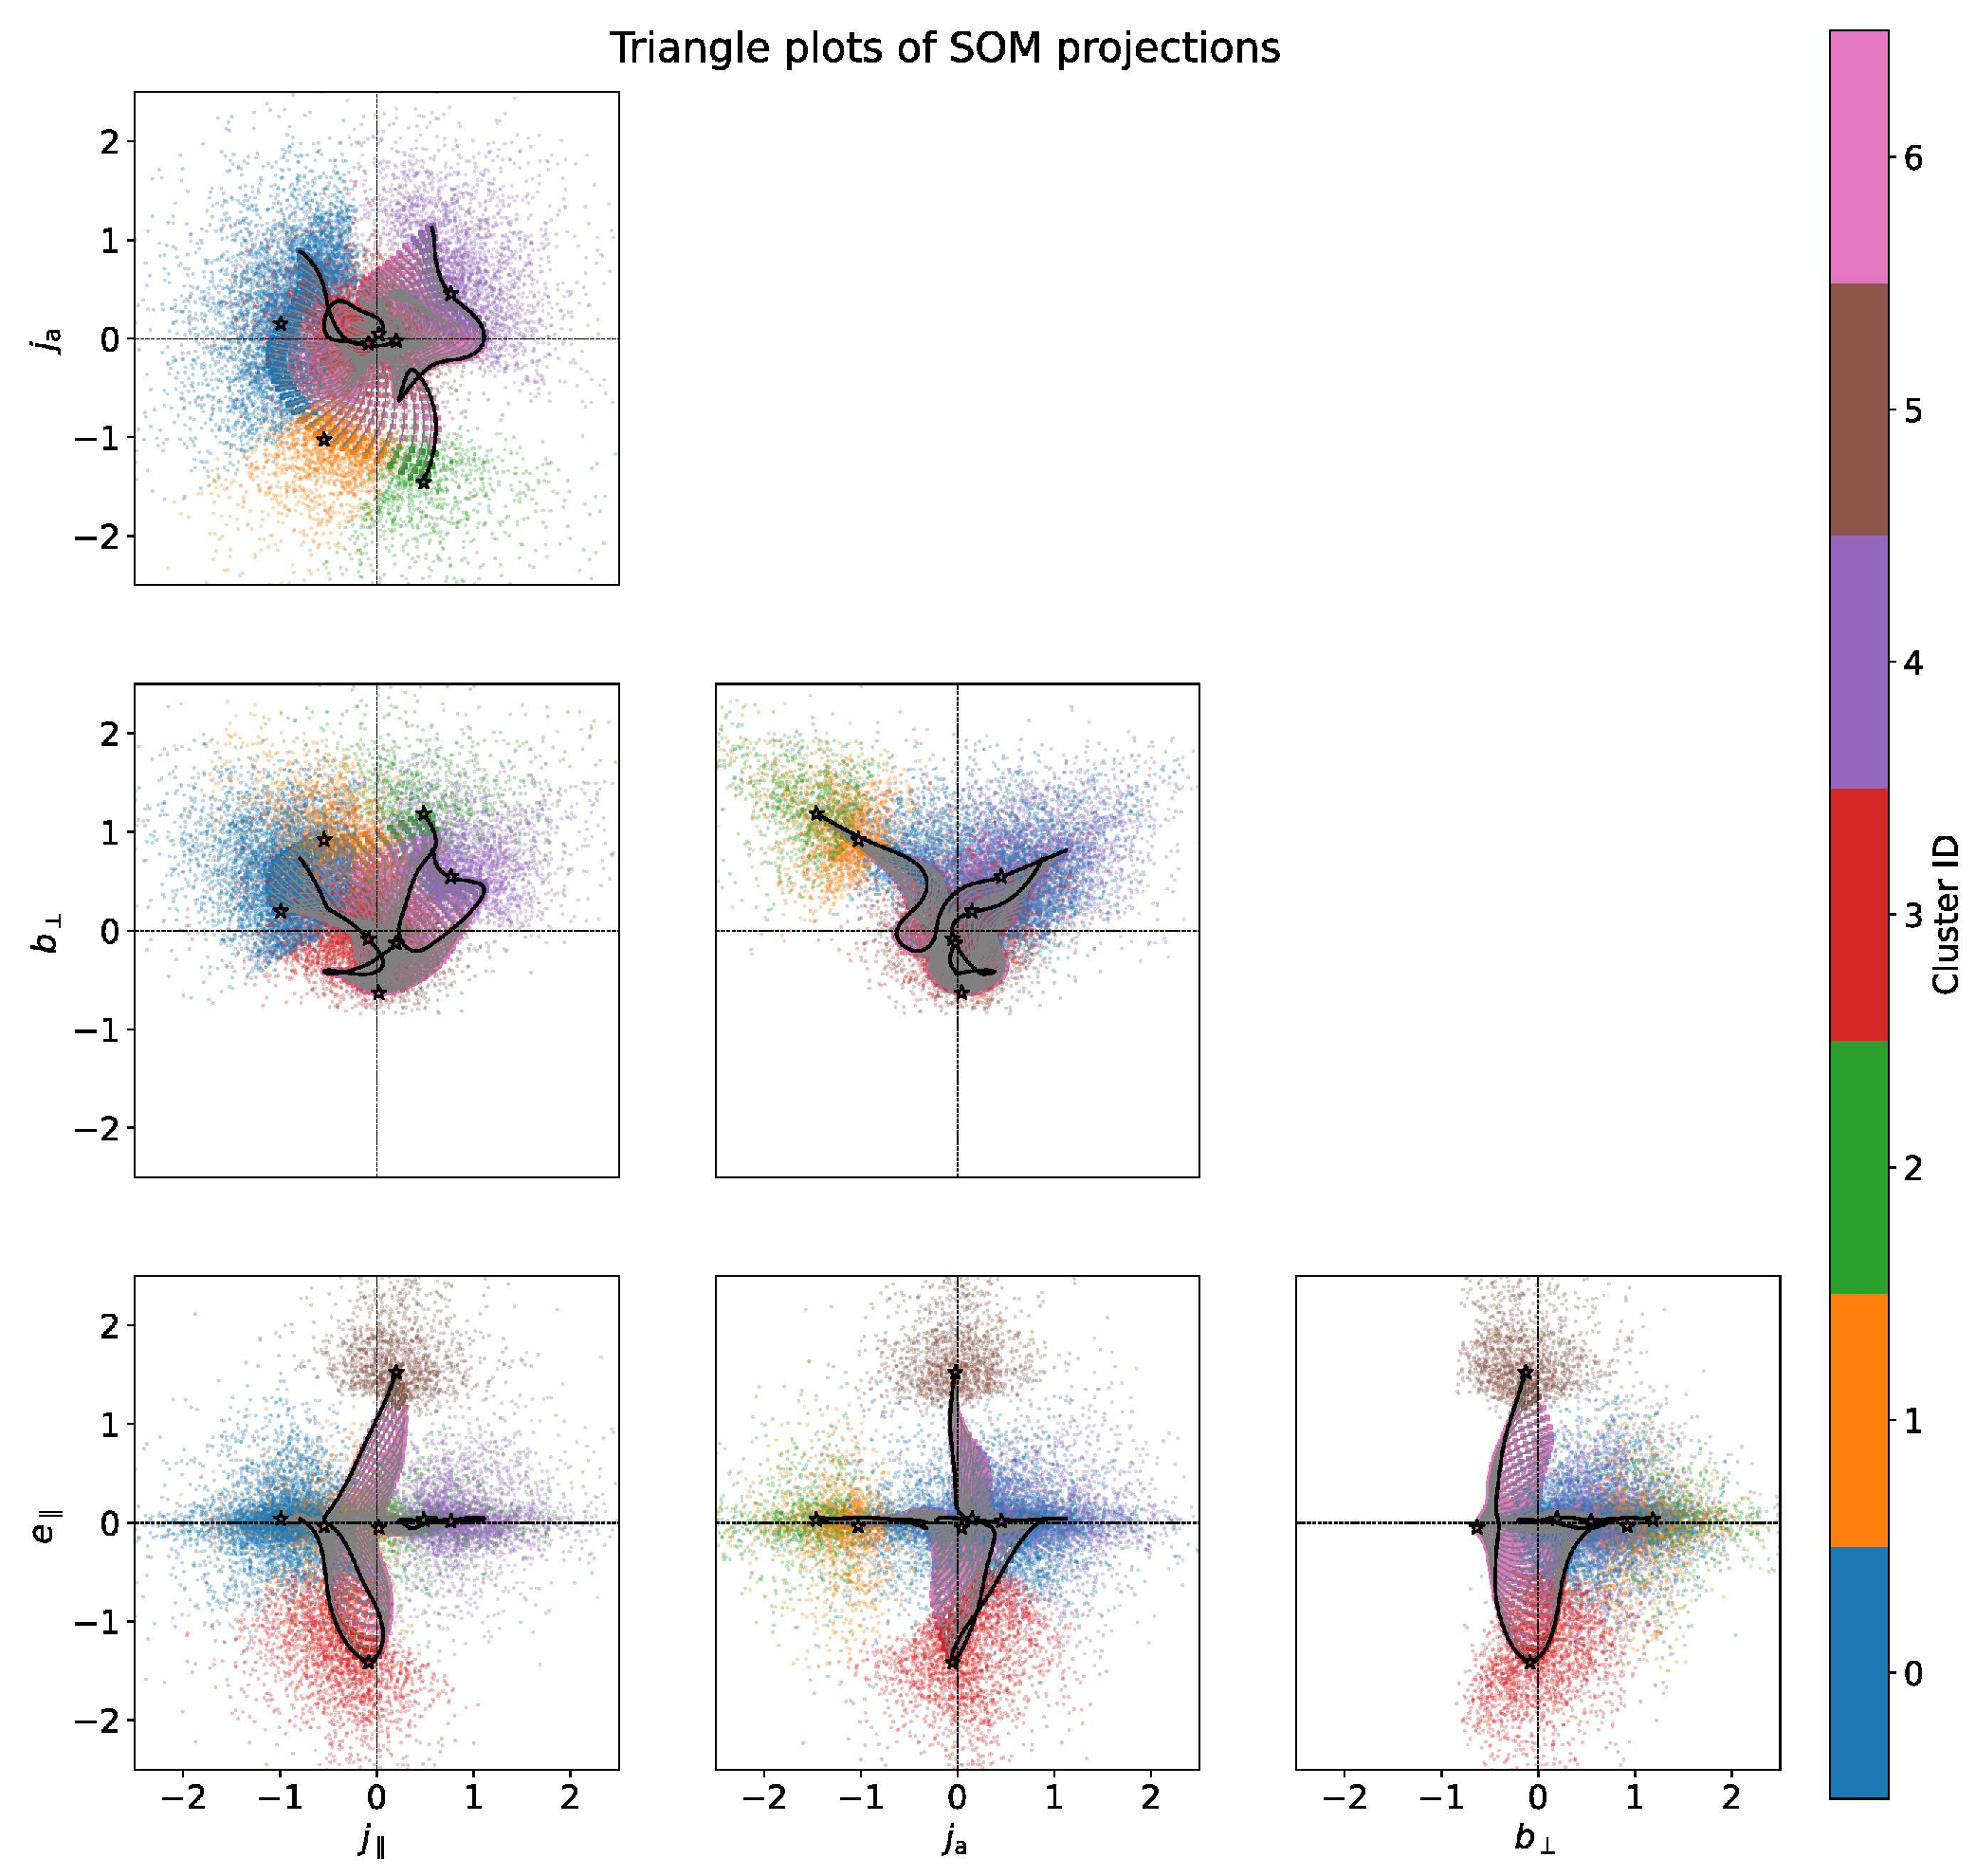
\includegraphics[width=0.9\linewidth]{Plasma_img/som_triangle.pdf}
    \caption{Scatter plots of SOM clusters (in the background; similar to Figure~\ref{fig:triangle}) and projections of the SOM lattice (in the foreground), where each square is a node, and the stars are locations of the centroids of each cluster.
    The gray lines represent connected nodes along the $X$-axis in Figure~\ref{fig:cluster_umap}.
    The two black curves show the horizontal boundaries of the map with $Y = 0$\ and $Y = 36$.}
    \label{fig:lattice_triangle}
\end{figure}

\begin{figure}[htbp]
    \centering
    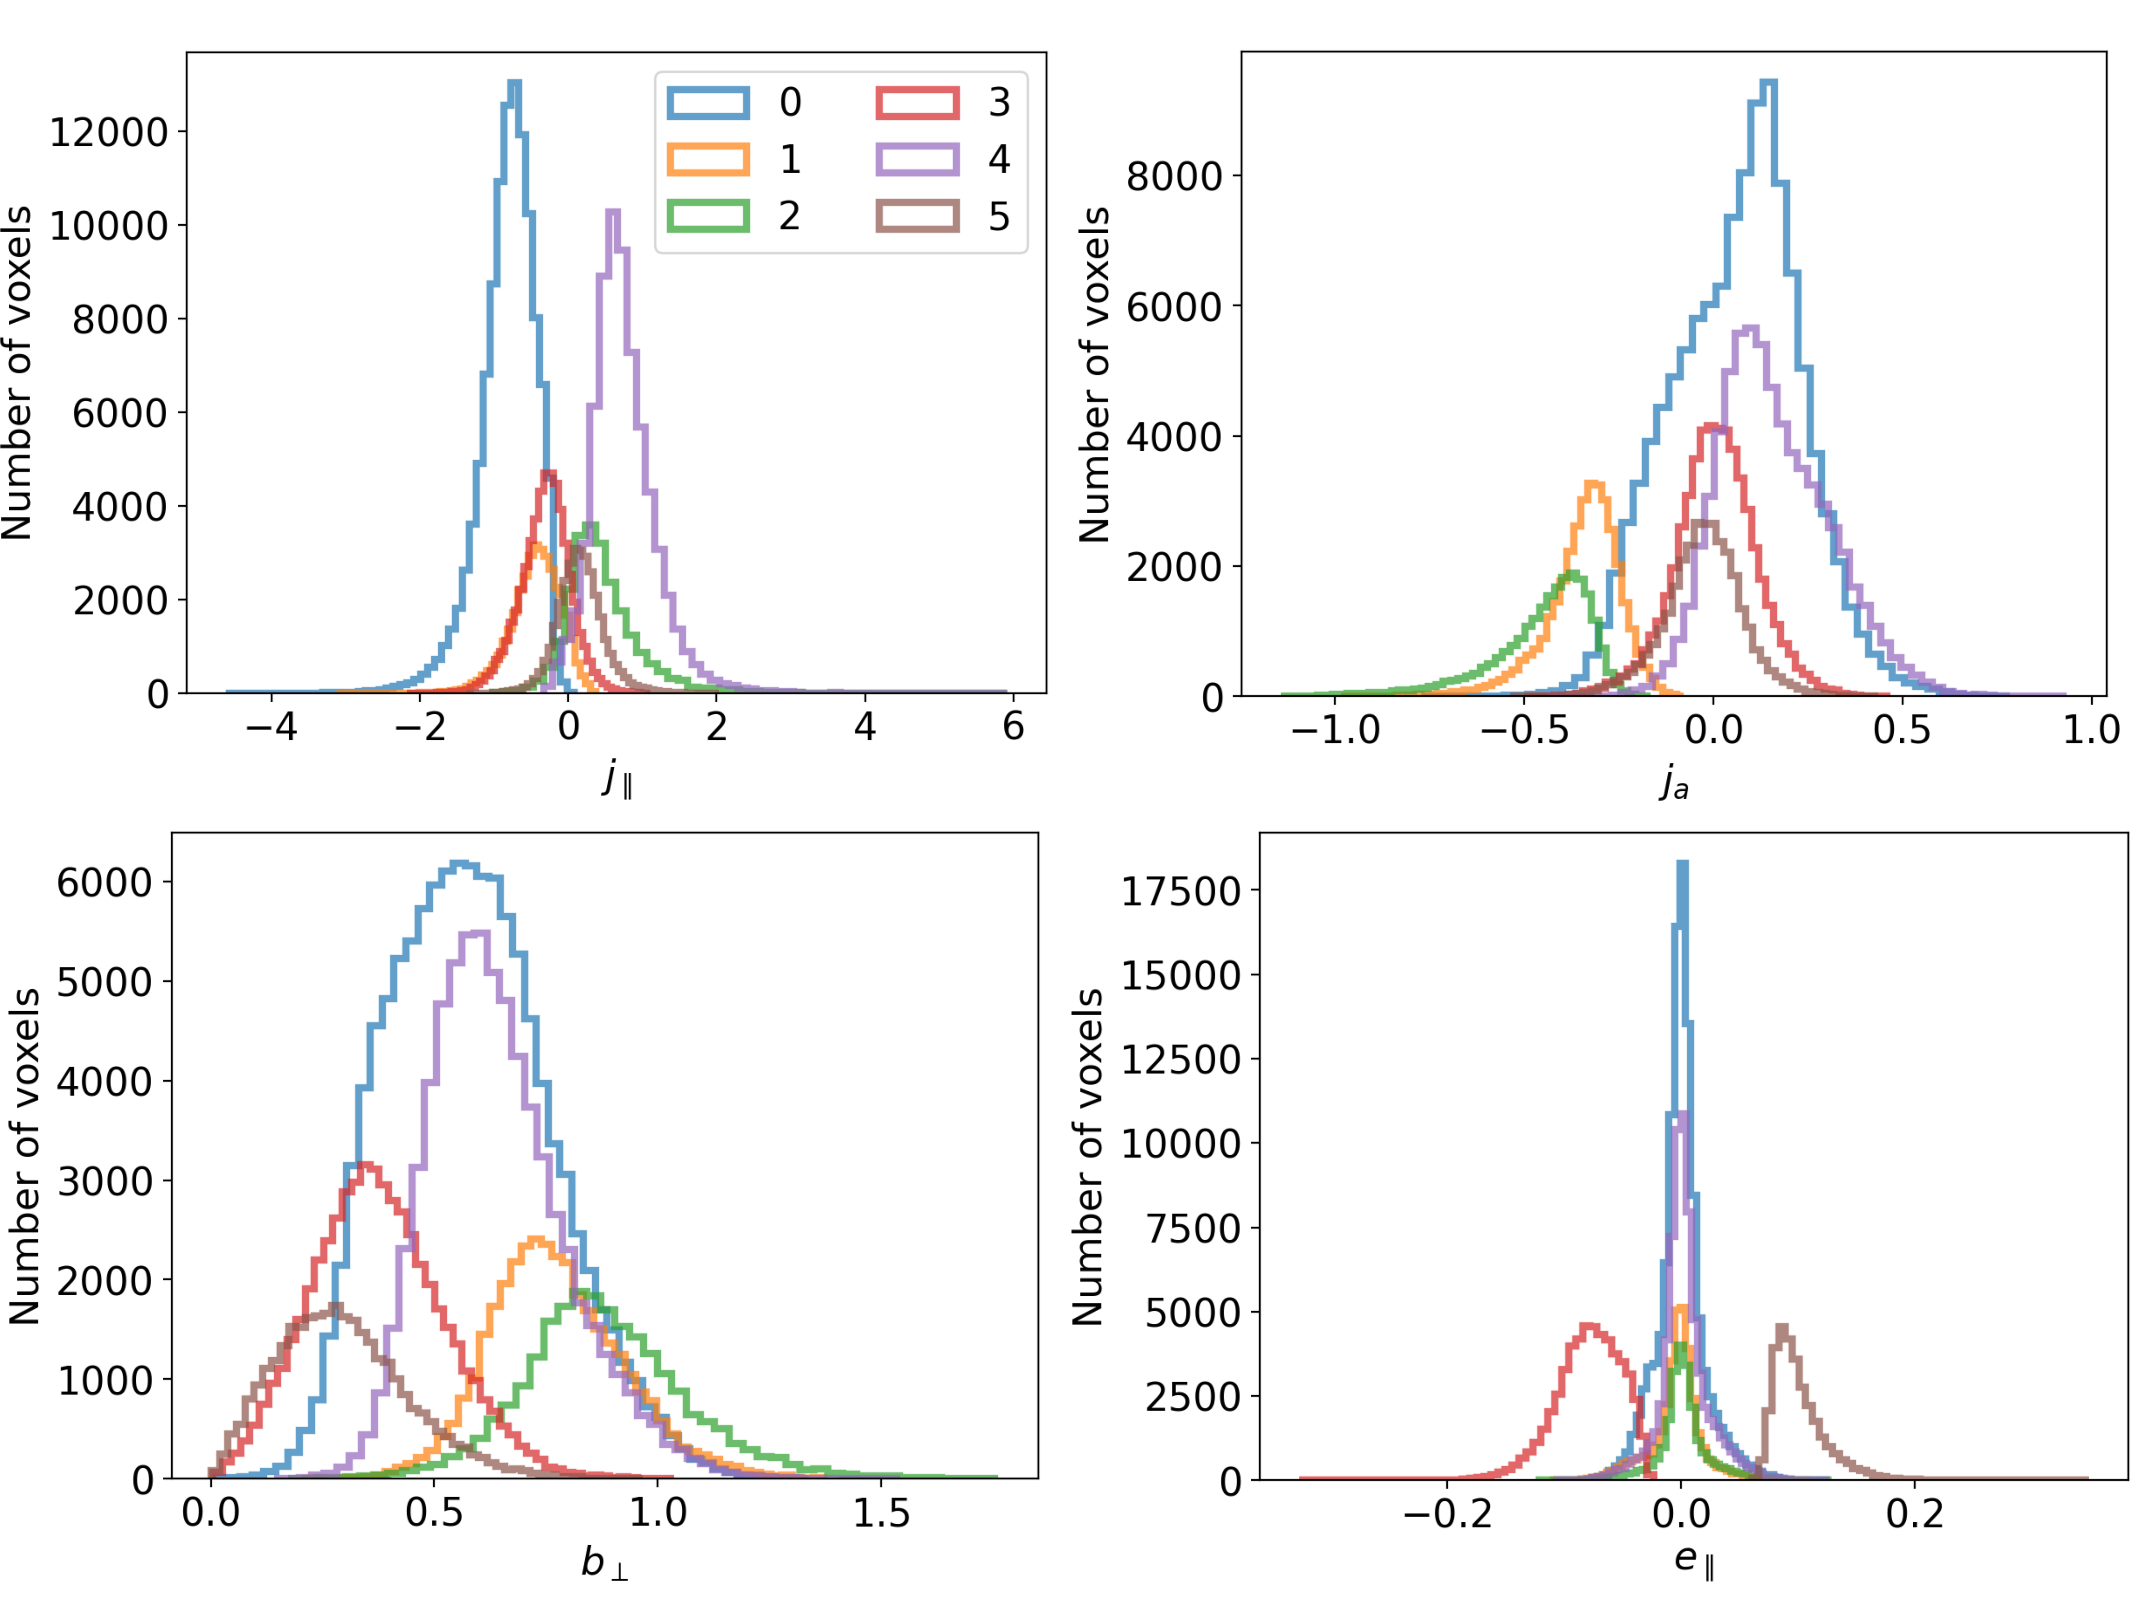
\includegraphics[width=0.7\linewidth]{Plasma_img/histograms.pdf}
    \caption{Histograms of each feature used in training, separated by clusters from Figure~\ref{fig:cluster_umap}. For clarity, cluster 6 has been omitted.}
    \label{fig:histograms}
\end{figure}

We perform several statistical analyses based on the fiducial SOM clusters to further explore the physics behind each cluster. For each of these analyses, we omit cluster 6, which only contains the background plasma.

Figure~\ref{fig:triangle} shows scatter plots between pairs of features used. A random sample of $10^5$\ data points is used, and cluster 6 (background) is omitted, to improve the clarity of the plots. The data points are quite clearly separated in a multi-dimensional space. For instance, clusters 0 (blue) and 4 (purple), as well as clusters 1 (orange) and 2 (green), are separated along the \jpar\,$=0$\ line. As we established in the main text, these clusters are either parts of the double sheet structures (clusters 1 and 2), or they are individual current sheets (clusters 0 and 4). Another correlation that we can see is in the \epar\ plots, where clusters 3 (red) and 5 (brown) are on opposite tail ends of the distribution. We also observe that the double current sheets tend to have markedly stronger \bperp\ than the rest of the data, pointing to the prominent peak in $B_{p1}$~seen in Figure~\ref{fig:single_double}.
Figure~\ref{fig:lattice_triangle} shows the same scatter plots as Figure~\ref{fig:triangle}, but with the projections of the SOM lattice plotted in the foreground, showing the non-linear topology of the lattice.
It can be used to read the non-linear combination of the feature-space parameters that the map uses for the clustering:
the major axis (i.e., slices along $X$) is mainly oriented along the $j_a$ feature but also captures variations in $e_\parallel$ in the top part of the map (for $Y \gtrsim 30$).
The minor axis (i.e., slices along $Y$) is somewhat oriented along $j_\parallel$ and $b_\perp$.
However, we emphasize that the real map is composed of a non-linear combination of the features and is, therefore, highly tangled in the feature space.

Figure~\ref{fig:histograms} shows histograms of each feature in our fiducial SOM run, separated by the clusters seen in Figure~\ref{fig:cluster_umap}. These histograms support the same conclusions as the scatter plots from Figure~\ref{fig:triangle}.

\subsubsection{Additional simulation data} \label{app:other-sims}

We compose a set of three 3D fully kinetic PIC simulations to study the formation and morphology of current sheets. The main text explores the details and results of the decaying turbulence box simulation.
Here, we investigate two other fully kinetic PIC simulations with similar conclusions as in the main text.

\centerline{\textbf{Reconnecting Harris current sheet}}

\begin{figure}[htbp]
    \centering
    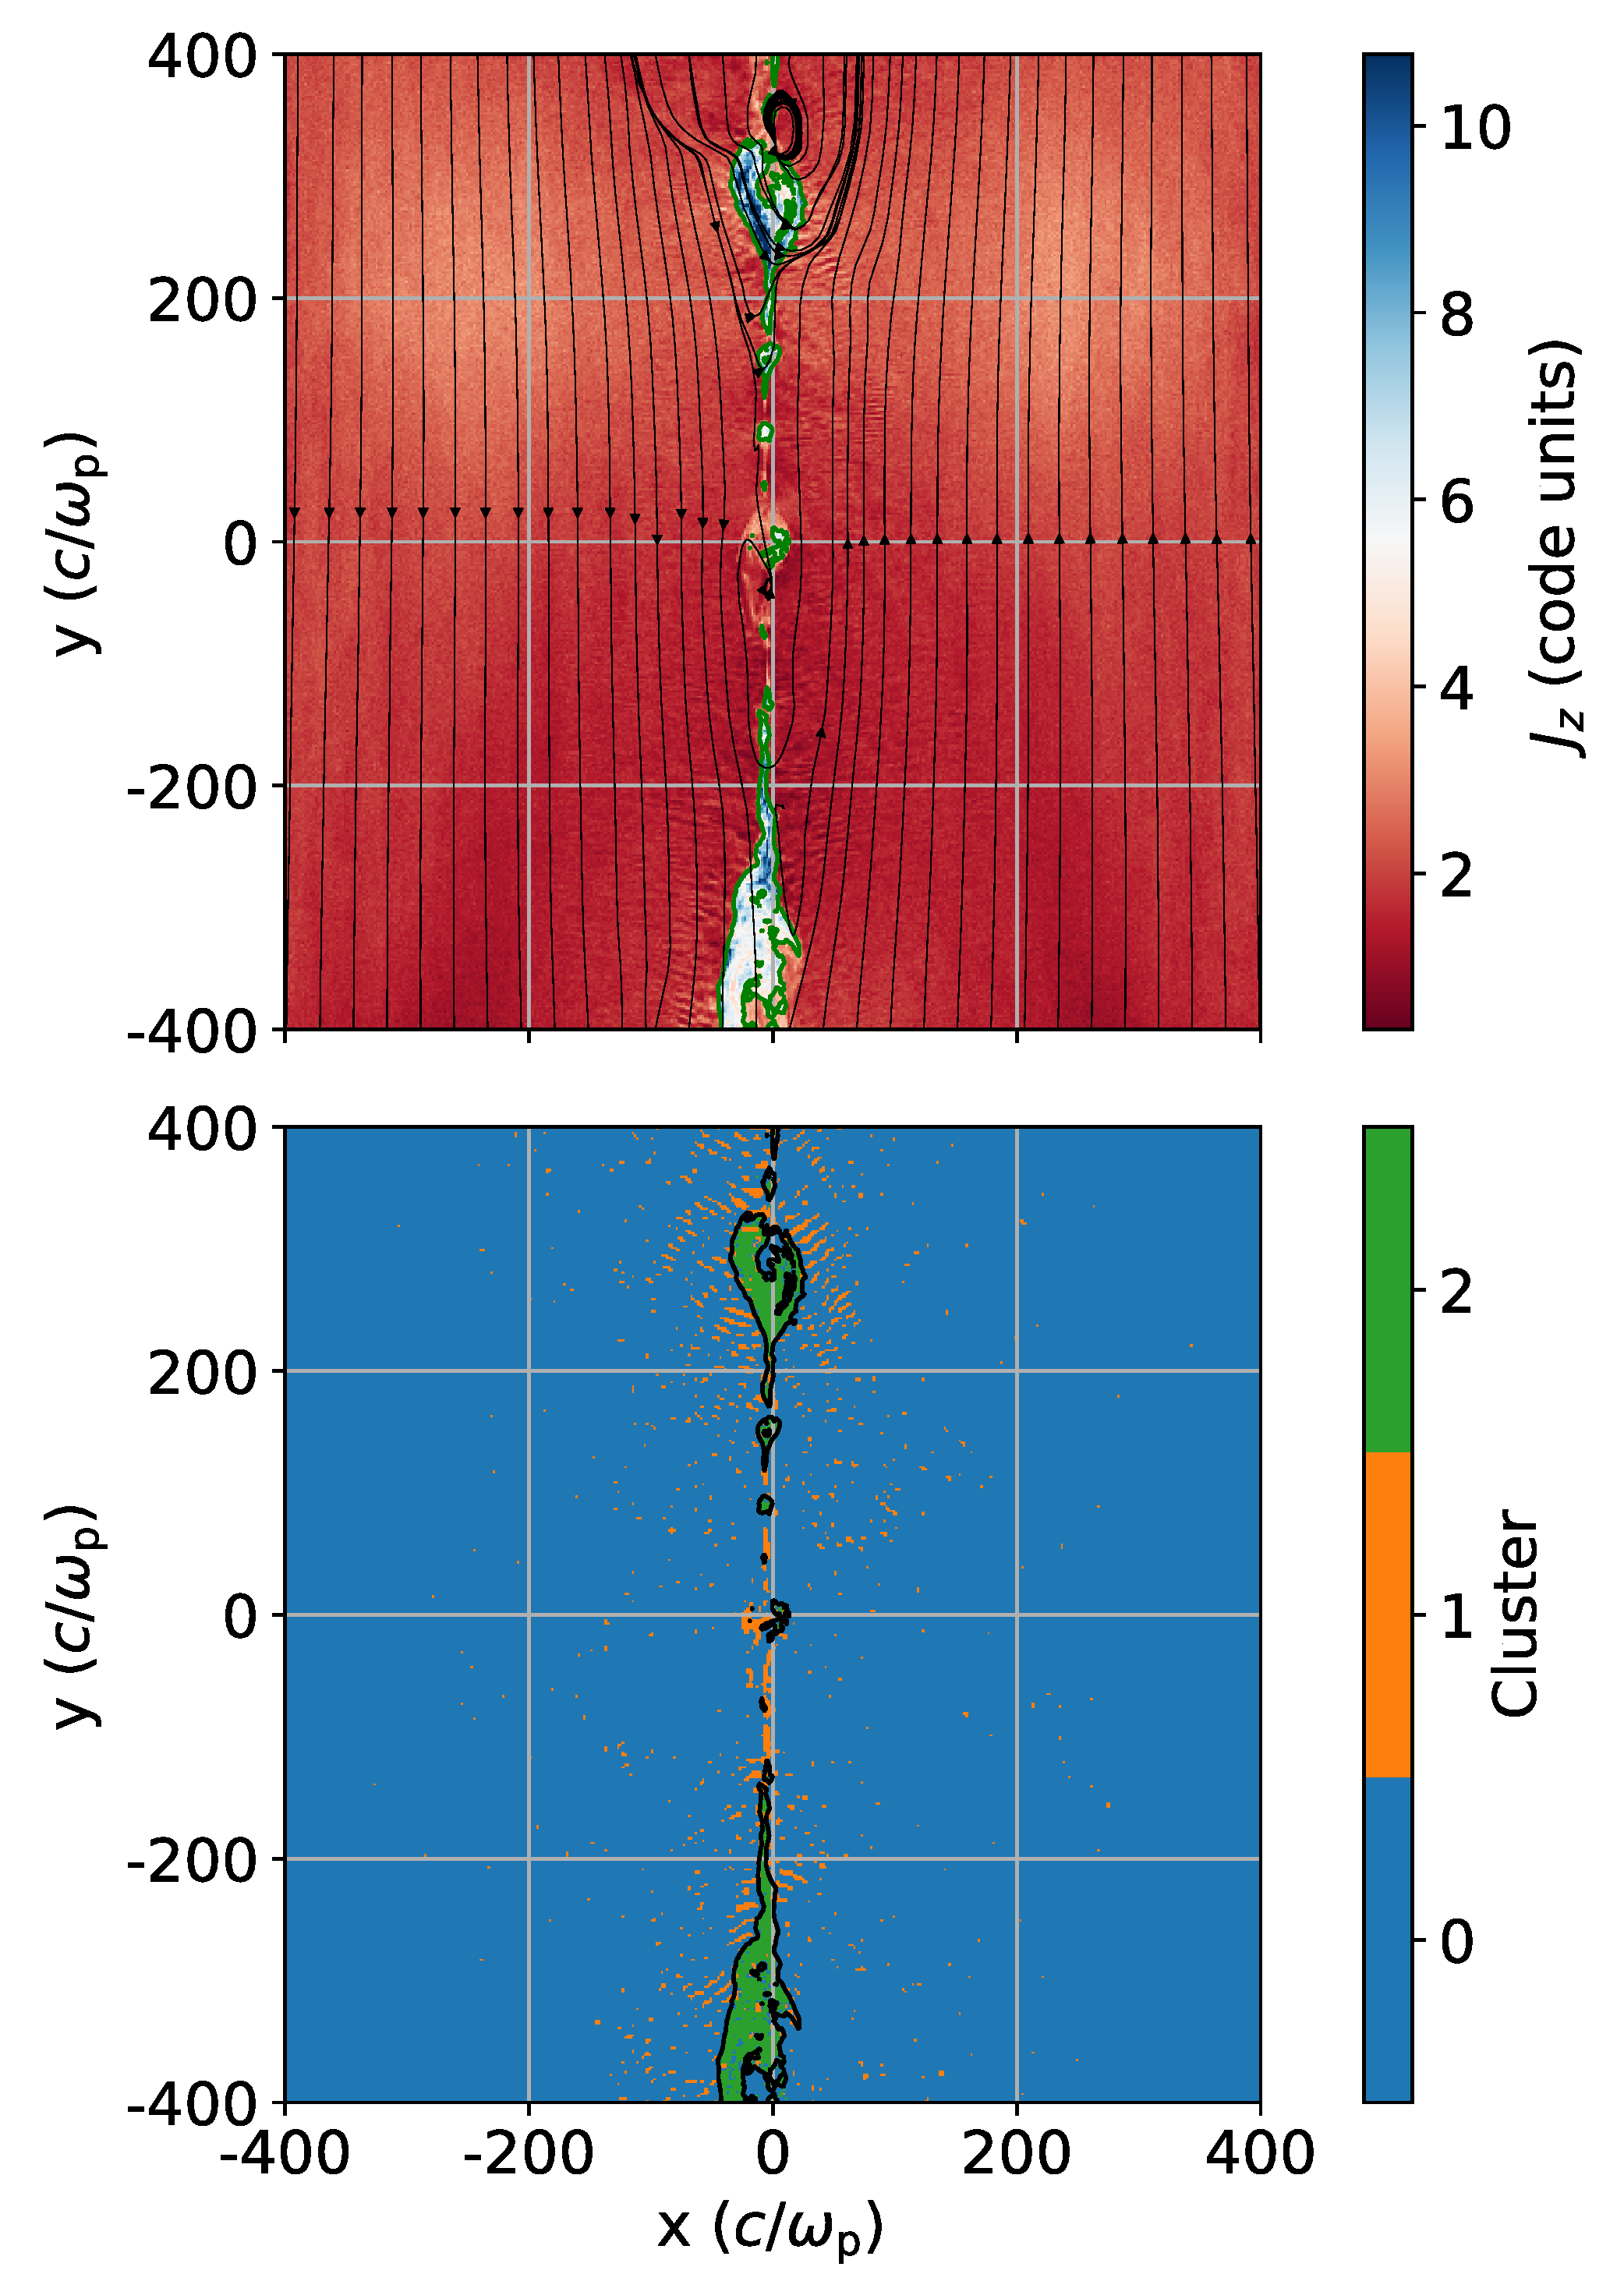
\includegraphics[height=0.8\textheight]{Plasma_img/figharris_key.pdf}
    \caption{$xy$-slice of current density along z-axis ($J_z$, top) vs.\ \awesom~clustering result (bottom) at $z = -40 c/\omega_{\rm p}$ for the Harris current sheet simulation. Streamlines in the top panel show in-plane magnetic field lines. Contours in both panels show regions where $J_z > 2 J_{\rm rms}$, representing the boundary of the Harris current sheet.}
    \label{fig:fig_harris}
\end{figure}

We use data from \citet{zhang_origin_2023} for an ideal simulation of a Harris current sheet.
The magnetic field $B_0$ is initialized to reverse from $+y$~to $-y$~across a current sheet at $x = 0$. The magnetization is $\sigma = 10$; a guide field of $B_g = 0.1 B_0$~along $z$~also presents. They initialize a cold $e^\pm$-pair plasma with rest-frame density, $n_0$, of 2 particles per cell per species.
Fresh plasma and magnetic flux are continuously injected along the $x$~direction of inflow.
The simulation domain covers $L_x = L_y = 2 L_z = 1600 c/\omega_{\rm p}$.
For ease of analysis, we select a cubic region of size $L = L_z = 800 c/\omega_{\rm p}$, centered on $x=y=z=0$.

We apply \awesom\ to the Harris sheet data with these parameters: $N = 10^6$, $X = 70$, $Y = 49$, and $\alpha_0 = 0.1$.
We use three features to train the model: $j_z$, \bperp, and \epar.
Given the idealized initial conditions, we do not recover the \jasym\ because only one current sheet is formed.
All other parameters are identical to the fiducial run in the main text.

Figure~\ref{fig:fig_harris} shows a $xy$-slice of an \awesom~clustering result of the Harris sheet.
In this idealized simulation, cluster 2 (green) has an almost-one-to-one correspondence with a current density threshold of $J_z > 2 J_{\rm rms}$, commonly used as a proxy for identifying current sheets in simulations \citep{zhdankin_statistical_2013}.
Cluster 0 (blue) accounts for the rest of the background plasma, and cluster 1 (orange) are locations with strong \epar.

\centerline{\textbf{Driven turbulence}}

\begin{figure}[htbp]
    \centering
    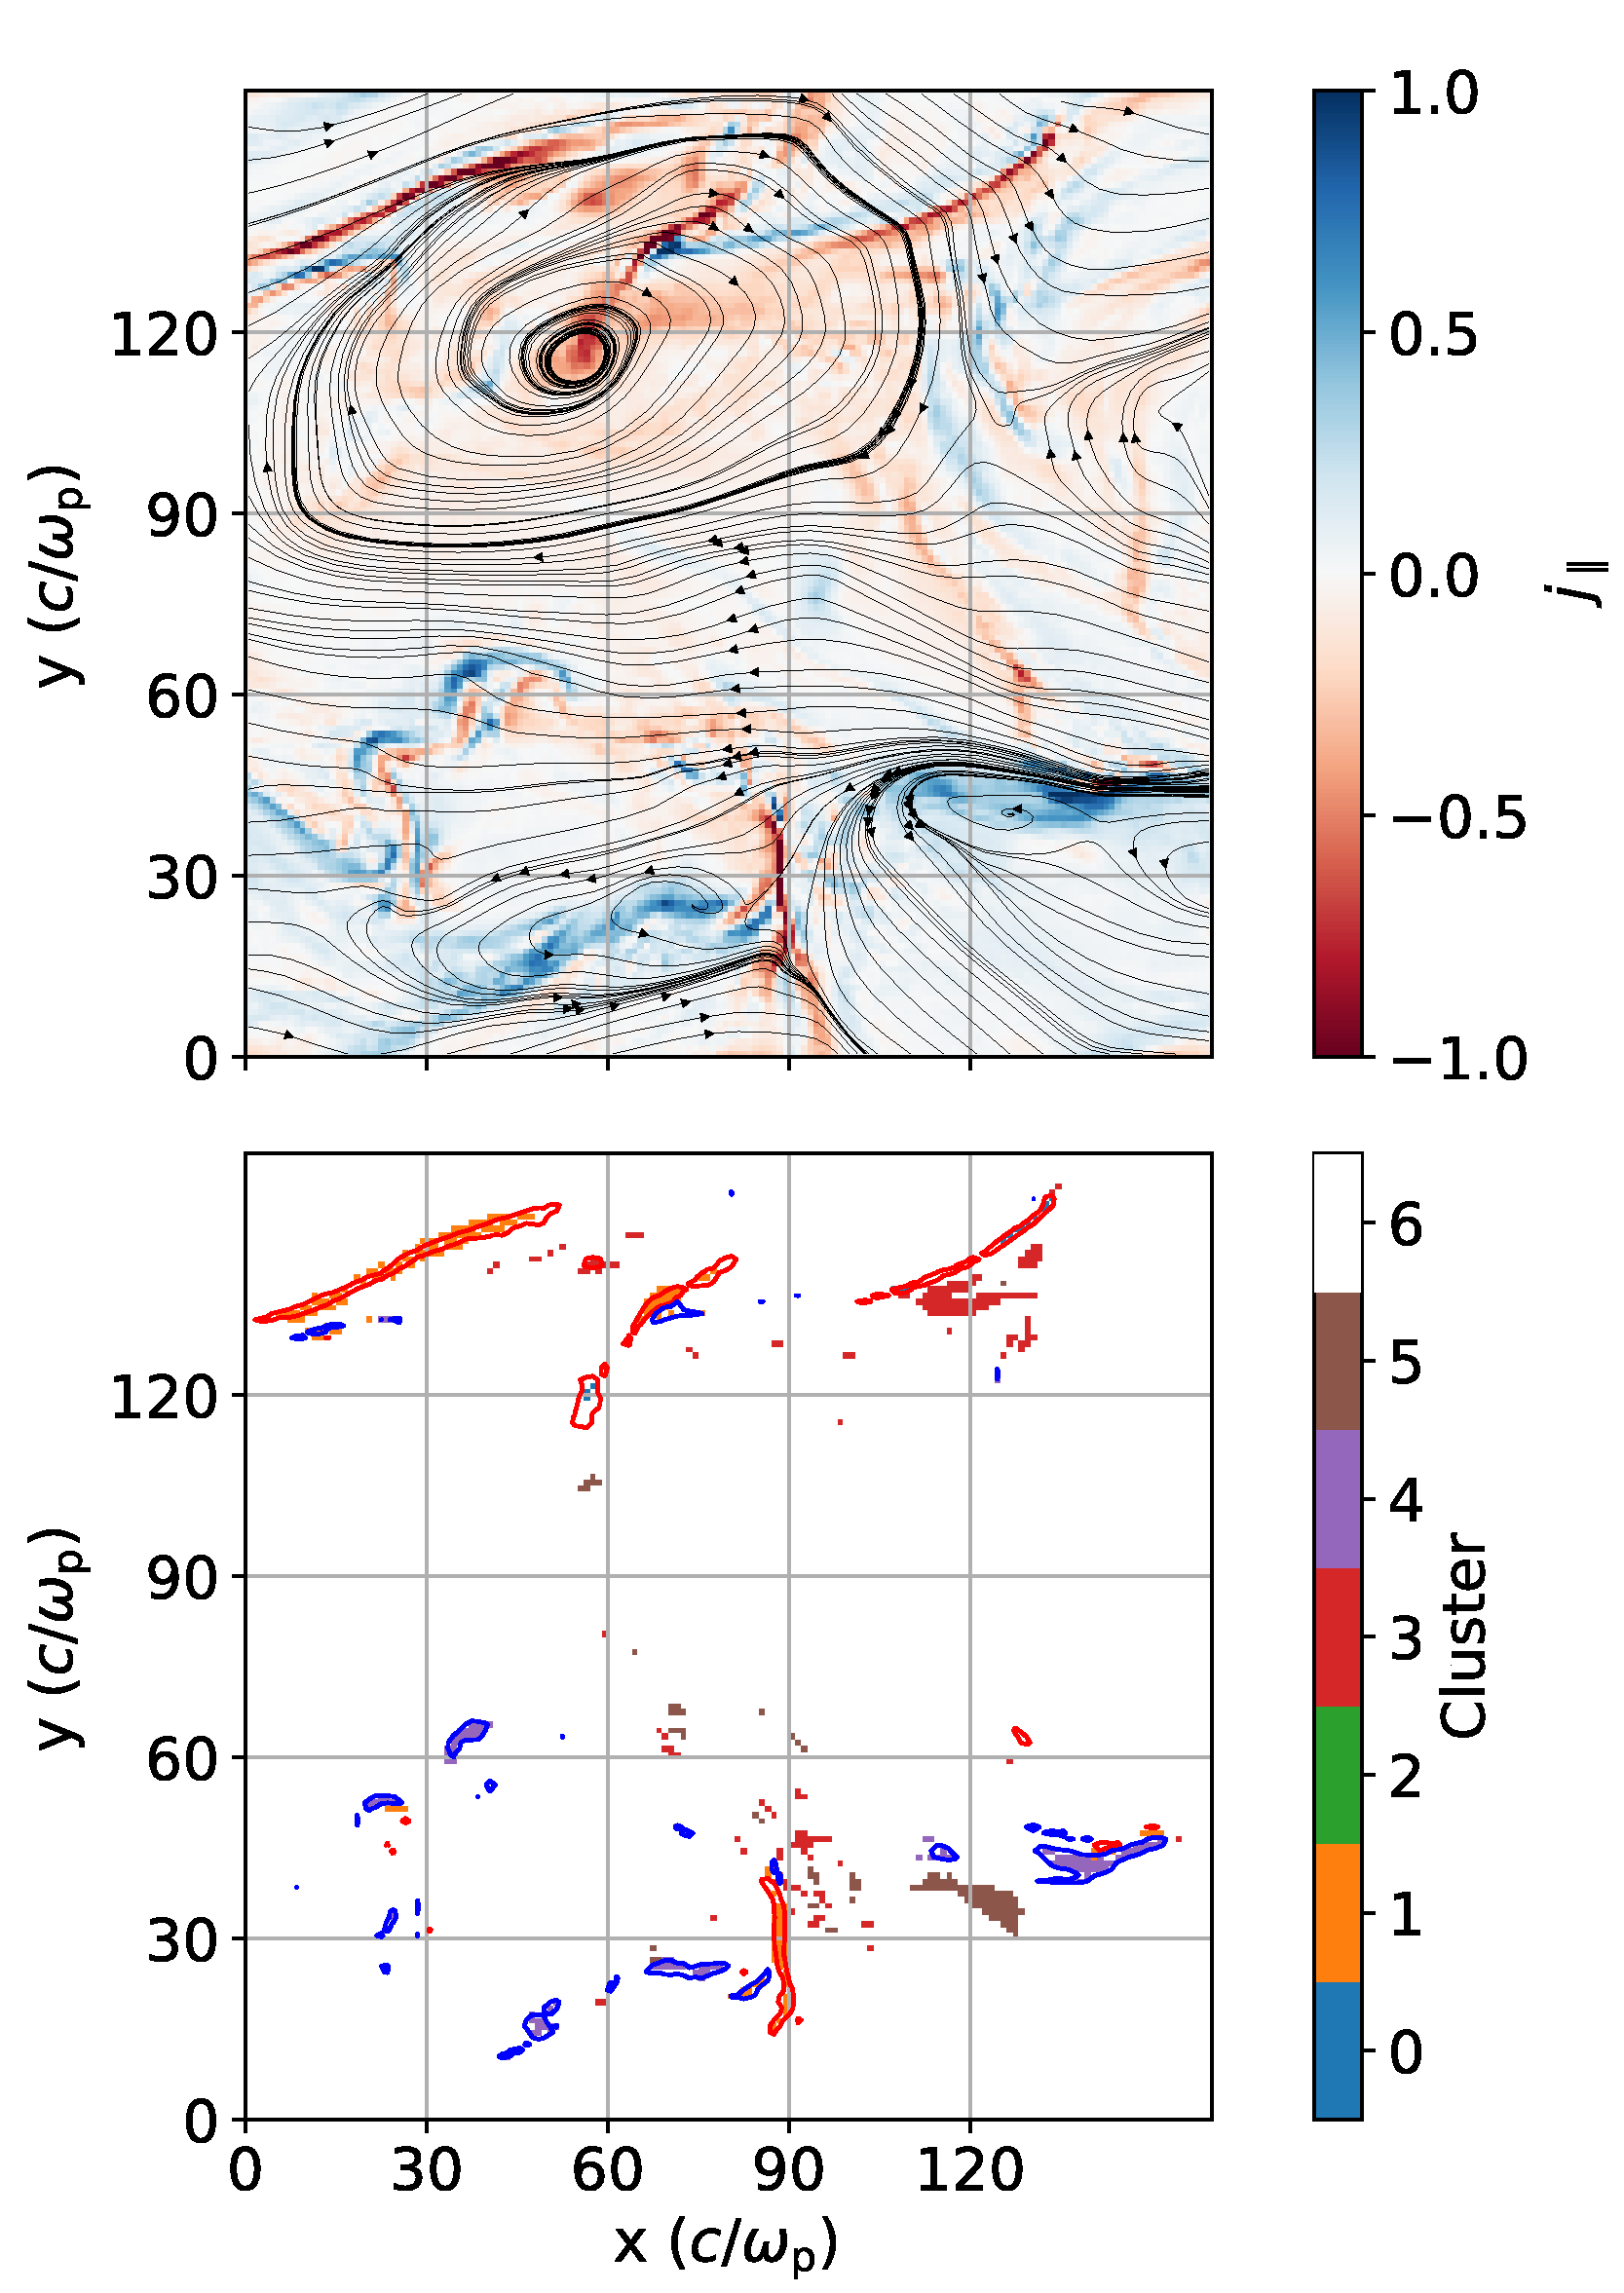
\includegraphics[height=0.8\textheight]{Plasma_img/figmerged_driven.pdf}
    \caption{$xy$-slice of \jpar~(top) vs.\ \awesom~clustering result (bottom) at $z = 120 c/\omega_{\rm p}$. Streamlines in the top panel show the in-plane magnetic field, $B_{xy}$. Red and blue contours in the bottom panel show locations where $j_{\parallel} < -3 \, j_{\parallel, \rm rms}$ and $j_{\parallel} > 3 \, j_{\parallel, \rm rms}$, respectively. The color of the clusters have the same physical meaning as in Figure~\ref{fig:merged_double}.}
    \label{fig:fig_driven}
\end{figure}

We also use snapshots from a continuously driven turbulence simulation \citep{nattila_radiative_2024}.
Similar to the freely-evolving turbulence case, the domain is a triply periodic cubic box of length $L = 640 c/\omega_{\rm p}$, which contains a neutral $e^\pm$-pair plasma with 8 particles per cell per species.
The domain has a magnetization of $\sigma = 10$ and is initialized with a uniform magnetic field $\mathbf{B}_0 = B_0 \hat{\mathbf{z}}$.
The turbulence is continuously excited by driving an external current with an oscillating Langevin antenna formalism \citep{tenbarge_oscillating_2014}.
The antenna has the following properties: driving scale $l_0 = L/2$, amplitude $\delta B / B_0 = 0.8$, frequency $\omega_{\rm ant}/\omega_{0} = 0.8$ (where $\omega_0 = 2\pi/t_0$ is the eddy-turnover frequency, and $t_0 = l_0/v_{\rm A}$ is the eddy-turnover time), and a decorrelation time of $\omega_{\rm dec} / \omega_0 = 0.6$.
The SOM presented below was trained on one snapshot of the simulation, taken at $t \approx 1.5\;l_0/c$, which exhibits a magnetic power spectrum  $\propto k_\perp^\alpha$ with a slope of $\alpha \approx -2$.

We downsample the dataset by a factor of four in each dimension such that $\Delta x = 4 c/\omega_{\rm p}$ and trained \awesom\ on the resulting data.
We set $N = 160^3$, $X = 91$, $Y = 37$, and $\alpha_0 = 0.1$ in \awesom\@.
Four features are used, similar to the freely evolving turbulence case: \jpar, \jasym, \bperp, and \epar.

Figure~\ref{fig:fig_driven} shows a $xy$-slice plot of this simulation with a SOM~realization after separation of single and double current sheets, as detailed in Section~\ref{subsec:separate}.
In general, the intermittent structures in this domain are identified by \awesom\@.
Cluster 0 (blue) and cluster 4 (purple) are single current sheets that are aligned and anti-aligned with $\mathbf{B}$, respectively.
Cluster 1 (orange) are double current sheets.
Meanwhile, cluster 3 (red) and cluster 5 (brown) are locations where \epar\ is high, and cluster 6 (white) are locations of the background plasma.
The volume-filling fraction of each cluster-of-interest (for clusters $k = 0, 1, 2, \ldots$) is: $n_{{\rm fill},\ k} \approx 0.09\%, 0.91\%, 0\%, 0.70\%, 0.37\%, 0.57\%, {\rm and}\ 97.36\%$.


Notably, the volume-filling fraction of the sheets is much smaller than that found in the freely-evolving turbulence simulation, $n_{\rm fill,0+1+4} \approx 1.37\%$.
Given the similar (down-sampled) resolution of both the decaying turbulence and driven turbulence box, such a discrepancy in volume-filling fractions may be explained by the different modes of perturbation, or by the size of the turbulence driver ($l_0 = L/2$, vs.\ $L/4$\ in the decaying turbulence simulation).
Alternatively, the difference seen here could be due to a transient turbulent effect such as a flare that is inadequately captured by individual snapshots.
The largest current sheets in the continuously driven turbulent domain could be sourced by the external driving mechanism, rather than the non-linear turbulent cascade, and, hence, we do not expect the double sheets to be as prominent in this simulation compared to the fiducial case presented in the main text.
Nevertheless, the analysis shows qualitatively similar results to the freely-evolving turbulence simulations.

\chapter{\texorpdfstring{\MakeUppercase{Understanding AGN-driven Turbulence in the Core of Elliptical Galaxies with Numerical Simulations}}{Understanding AGN-driven Turbulence in the Core of Elliptical Galaxies with Numerical Simulations}} \label{chap:sim}

\section{Background and motivation}
\subsection{The cooling flow problem in galaxy clusters}

In galaxy clusters, the intracluster medium (ICM) is diffuse and hot \citep[$n \sim 10^{-3}$\,cm$^{-3}$, $T \sim 10^7$--$10^8$\,K,][]{fabian_subsonic_1977,sarazin_x-ray_1986}.
At these temperatures, the ICM radiates via thermal bremsstrahlung in the form of X-ray emission and rapidly cools.
As the gas loses thermal pressure support, it is expected to flow toward the cluster core, collapse under self-gravity to form stars, and experience runaway cooling \citep[see, e.g.,][]{fabian_cooling_1994}.
However, X-ray spectroscopy of galaxy cluster cores revealed a deficiency in the amount of cool gas and the rate of star formation that would otherwise be expected given such a flow, a discrepancy known as the \textit{cooling flow problem} \citep{peterson_high-resolution_2003, peterson_x-ray_2006, odea_infrared_2008}.
This deficiency suggests that some form of heating takes place within the ICM that slows or even suppresses the cooling flow.
The most likely source of this heating is active galactic nucleus (AGN) feedback in the form of radio jets \citep{mcnamara_heating_2007,fabian_observational_2012}.

\begin{figure}
    \centering
    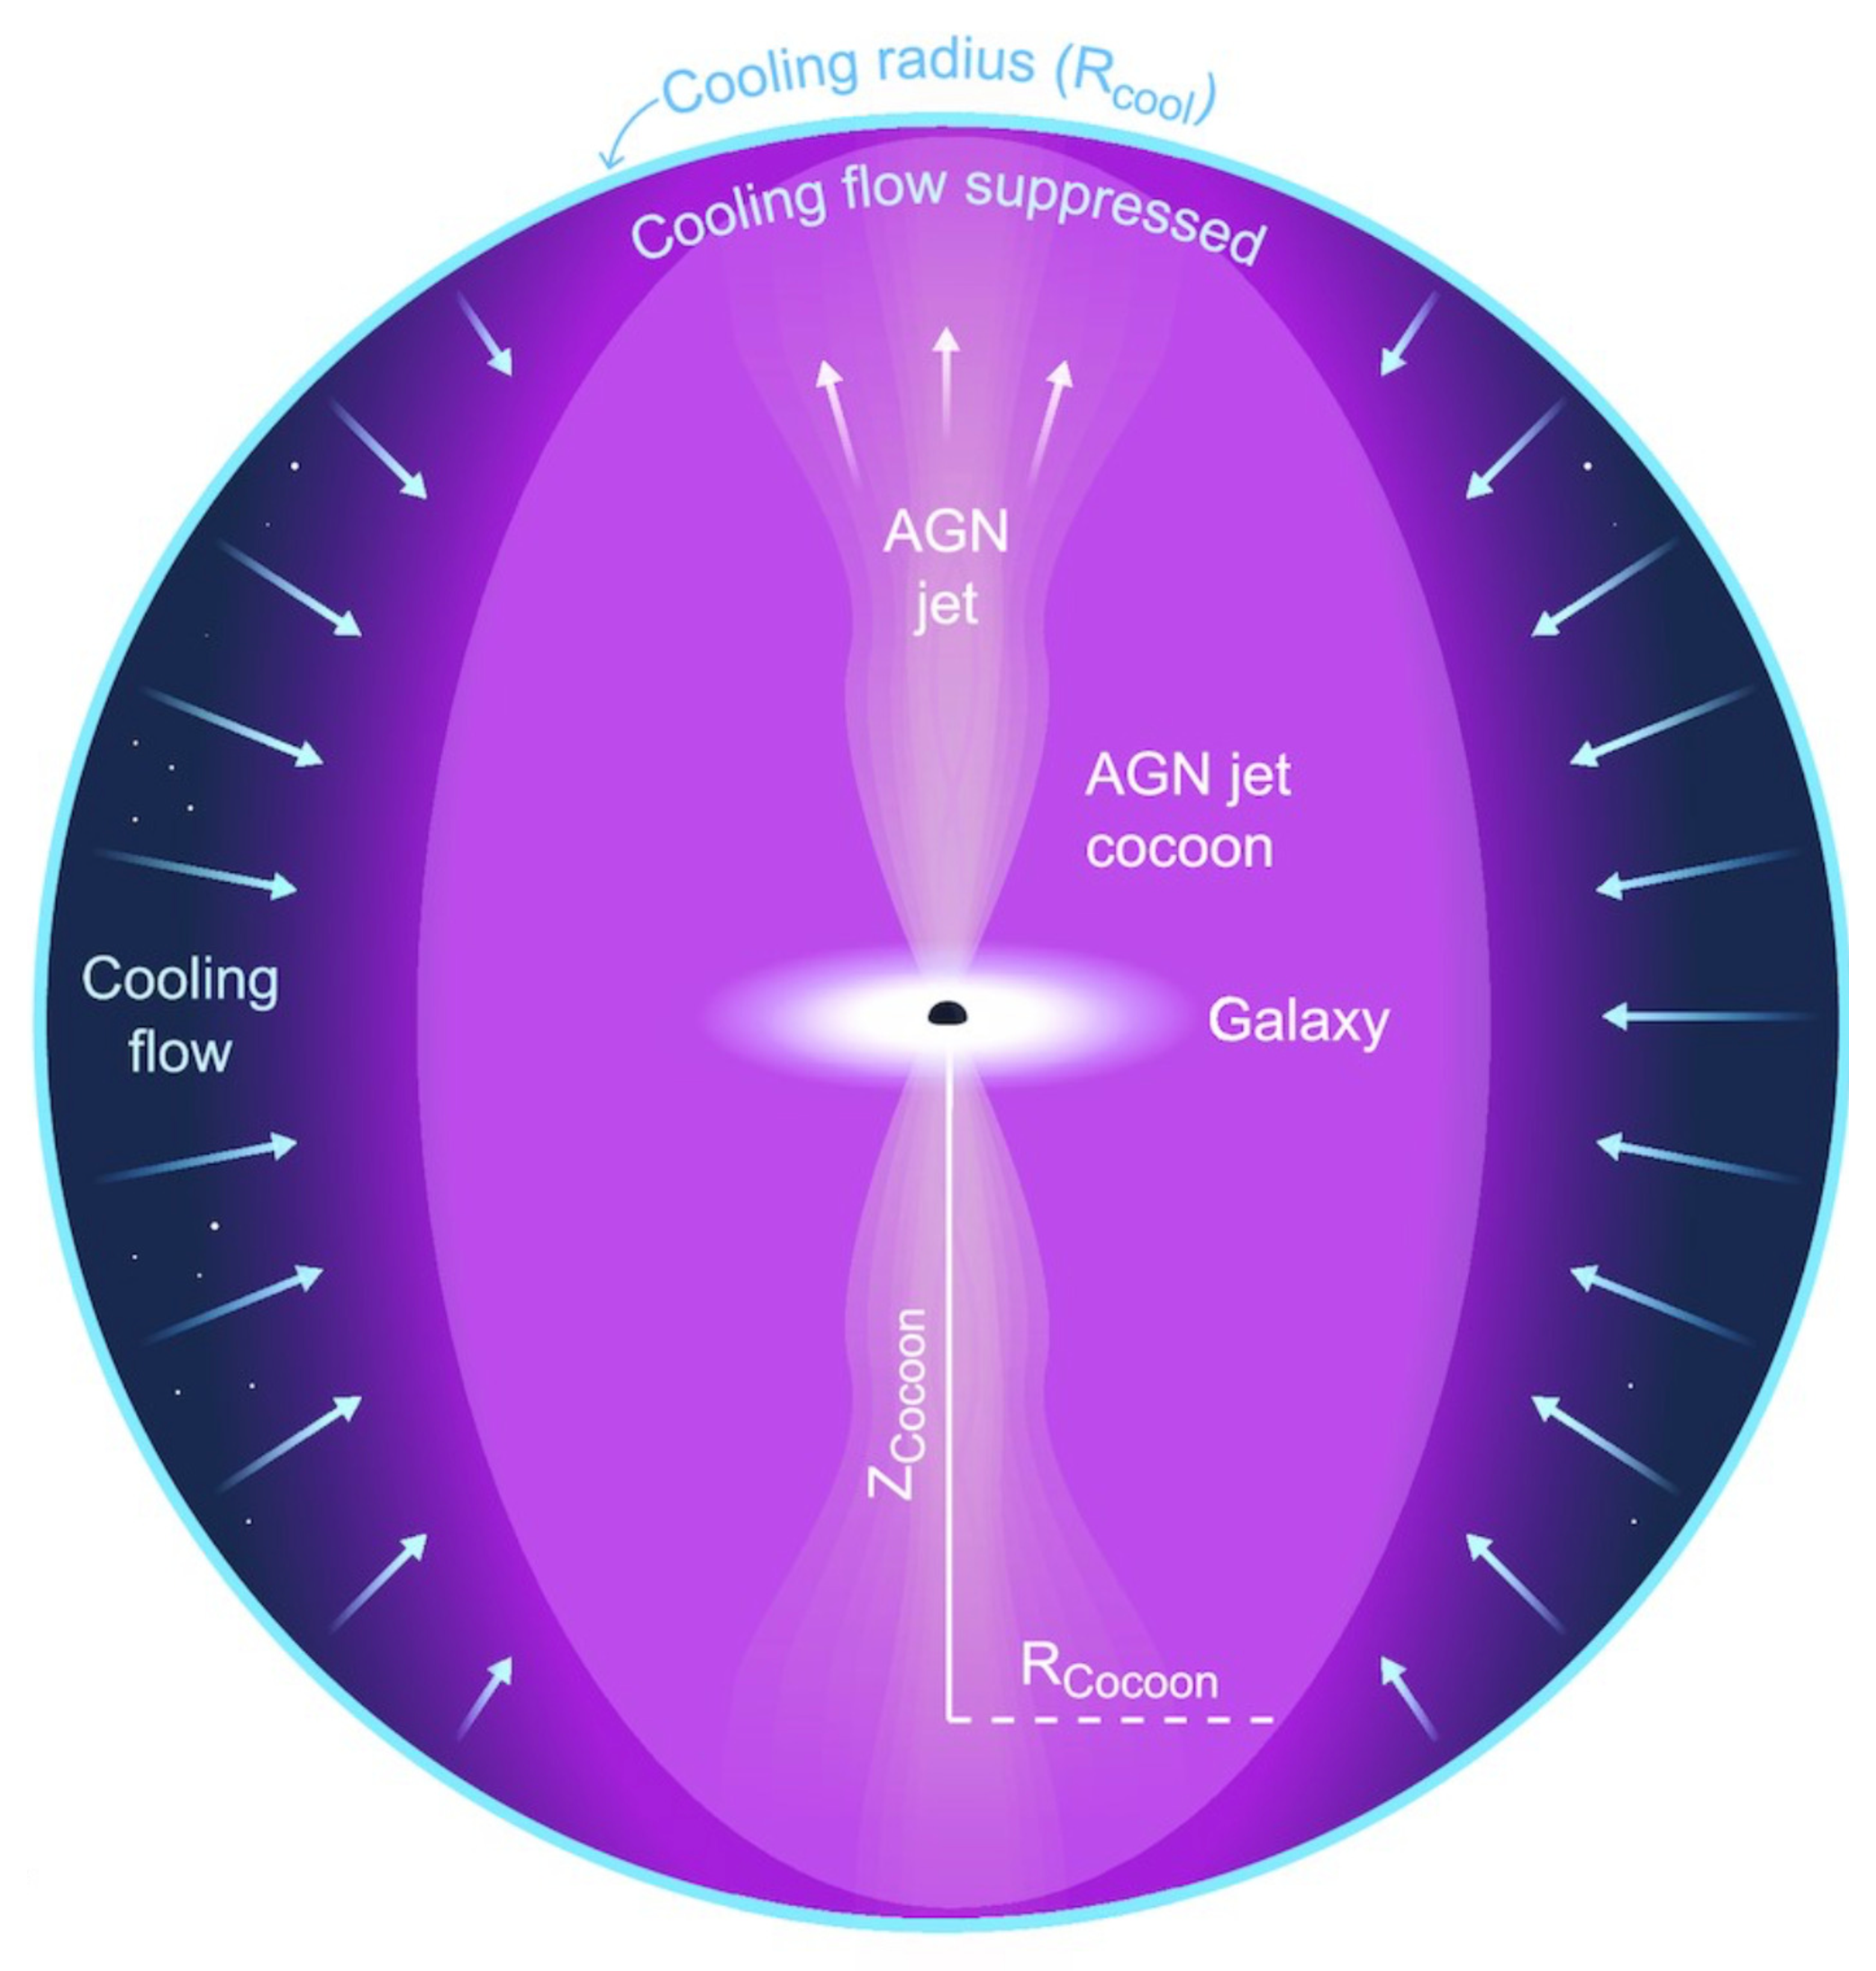
\includegraphics[width=0.8\linewidth]{Sim_img/AGN-cycle.pdf}
    \caption{Adapted from Figure 7 of \citet{su_which_2021}; illustration of the feeding-feedback cycle in AGNs. Jet feedback drives turbulence in the circumgalactic medium (CGM) and facilitates gas mixing, which heats the galaxy at kpc scales. The mixture of warm gas continues to cool and cascade toward the plane of the galaxy. The gas ends up in an accretion disk perpendicular to the jet direction, and a fraction of it is accreted, while the rest interacts with the central engine and is launched outward via AGN jets, repeating the cycle.}
    \label{fig:multiscale-accretion}
\end{figure}

Many galaxy clusters harbor extended radio emission from the central AGN jet.
For example, the Virgo cluster (which hosts the galaxy M87 at its center) and the Centaurus cluster both have radio jets extending beyond $\sim 10$\,kpc from the cluster core.
Others, like Perseus, are known for X-ray cavities in the ICM, which are thought to be inflated by AGN jets and then rise away from the cluster core \citep{fabian_chandra_2000}.
The hot and energetic jet material collides with the surrounding medium and drives turbulence in the ICM, providing further kinetic pressure support against a cooling flow \citep{hitomi_collaboration_atmospheric_2018}.
These observations identify AGN jets as the likely source of heating, but leave open how jet energy is deposited into the gas and transported across scales to the galaxy core.

Because AGN jet power ultimately depends on gas accretion onto the central SMBH, the accretion flow is inextricably linked to the jet feedback that suppresses the cooling flow.
During periods of weak feedback, pressure support decreases, leading to a higher cooling rate and more accretion.
This large amount of matter accumulates in the accretion disk, extracting more energy from the black hole, which begins a period of strong jet feedback.
As the AGN jet pushes outward and collides with the surrounding medium, it heats up the galaxy, effectively shutting down cooling.
Without cooling, accretion is quenched, and the black hole goes into a quiescent phase, starting the cycle again.
Figure~\ref{fig:multiscale-accretion} shows an illustration, adapted from Fig.~7 of \citet[][]{su_which_2021}, of the feeding-feedback cycle in AGNs.

\subsection{The gap in our theoretical understanding of meso-scale accretion flows and their connection to AGN feeding and feedback}

AGN feedback depends strongly on the accretion state of the central SMBH\@.
Low-luminosity AGNs (LLAGNs), such as M87$^{\star}$ and Sagittarius A$^{\star}$, accrete matter at much lower rates than the theoretical Eddington limit ($\dot{M}_{\rm BH} \ll \dot{M}_{\rm Edd}$), while quasars accrete matter rapidly ($\dot{M}_{\rm BH} \sim \dot{M}_{\rm Edd}$).
At low accretion rates, feedback is mainly provided by the SMBH-driven jet---the \textit{radio-mode feedback}; at high accretion rates, feedback is more complex, but often dominated by radiation-driven pressure from the large amount of matter being actively accreted \citep[e.g.,][]{cielo_agn_2018}---the \textit{quasar-mode feedback}.

This chapter focuses on radio-mode feedback and the regulation of quiescent elliptical galaxies by AGN jets, with M87 as the central example.
M87 is the central galaxy of the Virgo cluster and hosts a SMBH \citep[$M_{\rm BH} \approx 6.5\times10^9\, M_{\odot}$;][]{eht_one}.
Because X-ray observations of AGNs struggle to probe the region near the SMBH \citep[e.g.,][]{snios_detection_2019}, $\dot{M}_{\rm BH}$ is often estimated using the Bondi accretion model \citep[][]{bondi_spherically_1952}.
For M87, however, estimates of \mdotbh\ from AGN luminosity and EHT observations are several orders of magnitude below the Bondi estimate \citep[][]{russell_radiative_2013,eht_eight}.
Follow-up X-ray observations also show that the density and temperature profiles inside the Bondi radius of M87 do not agree with the predicted profiles of Bondi accretion \citep[e.g.,][]{russell_inside_2015}.
In addition, M87 hosts multiphase gas with an additional $T \sim 10^4\,K$\ component, including gas observed in a disky structure \citep[e.g.,][]{walsh_m87_2013,lu_ring-like_2023}.
These discrepancies suggest that Bondi accretion is not the correct assumption for M87 or many other LLAGNs.

Despite evidence against the Bondi model, many state-of-the-art cosmological simulations still employ this framework to approximate the amount of feedback produced by galaxies \citep[e.g.,][]{dave_simba_2019,pakmor_millenniumtng_2023}.
At the opposite end of the spatial scale, general relativistic magnetohydrodynamic (GRMHD) simulations have successfully revealed the complex dynamics of the accretion flows near the event horizon, and their results generally agree with recent EHT observations of the accretion flows onto M87$^{\star}$ and Sagittarius A$^{\star}$ \citep{eht_one,eht_sgt_one}.
These simulations, however, are often initialized with a simple idealized torus inside a toroidal magnetic field \citep[e.g.,][]{white_structure_2020,kaaz_nozzle_2023}.
Such initial conditions are simple to set up, but lack physical motivation, and the results have been shown to be sensitive to the exact starting conditions \citep[see][]{davis_magnetohydrodynamics_2020}.
The work presented in this chapter addresses the gap between observations and simulations by studying multiphase accretion flows through eight orders of magnitude in scale.
By reaching the inner accretion disk region of the SMBH, it also provides physically motivated initial and boundary conditions for future GRMHD simulations, whose results can then be directly compared to observations made by the EHT\@.
Figure~\ref{fig:theory-gap} summarizes the field's need for this connection between resolved simulations and observations.

\begin{figure}
    \centering
    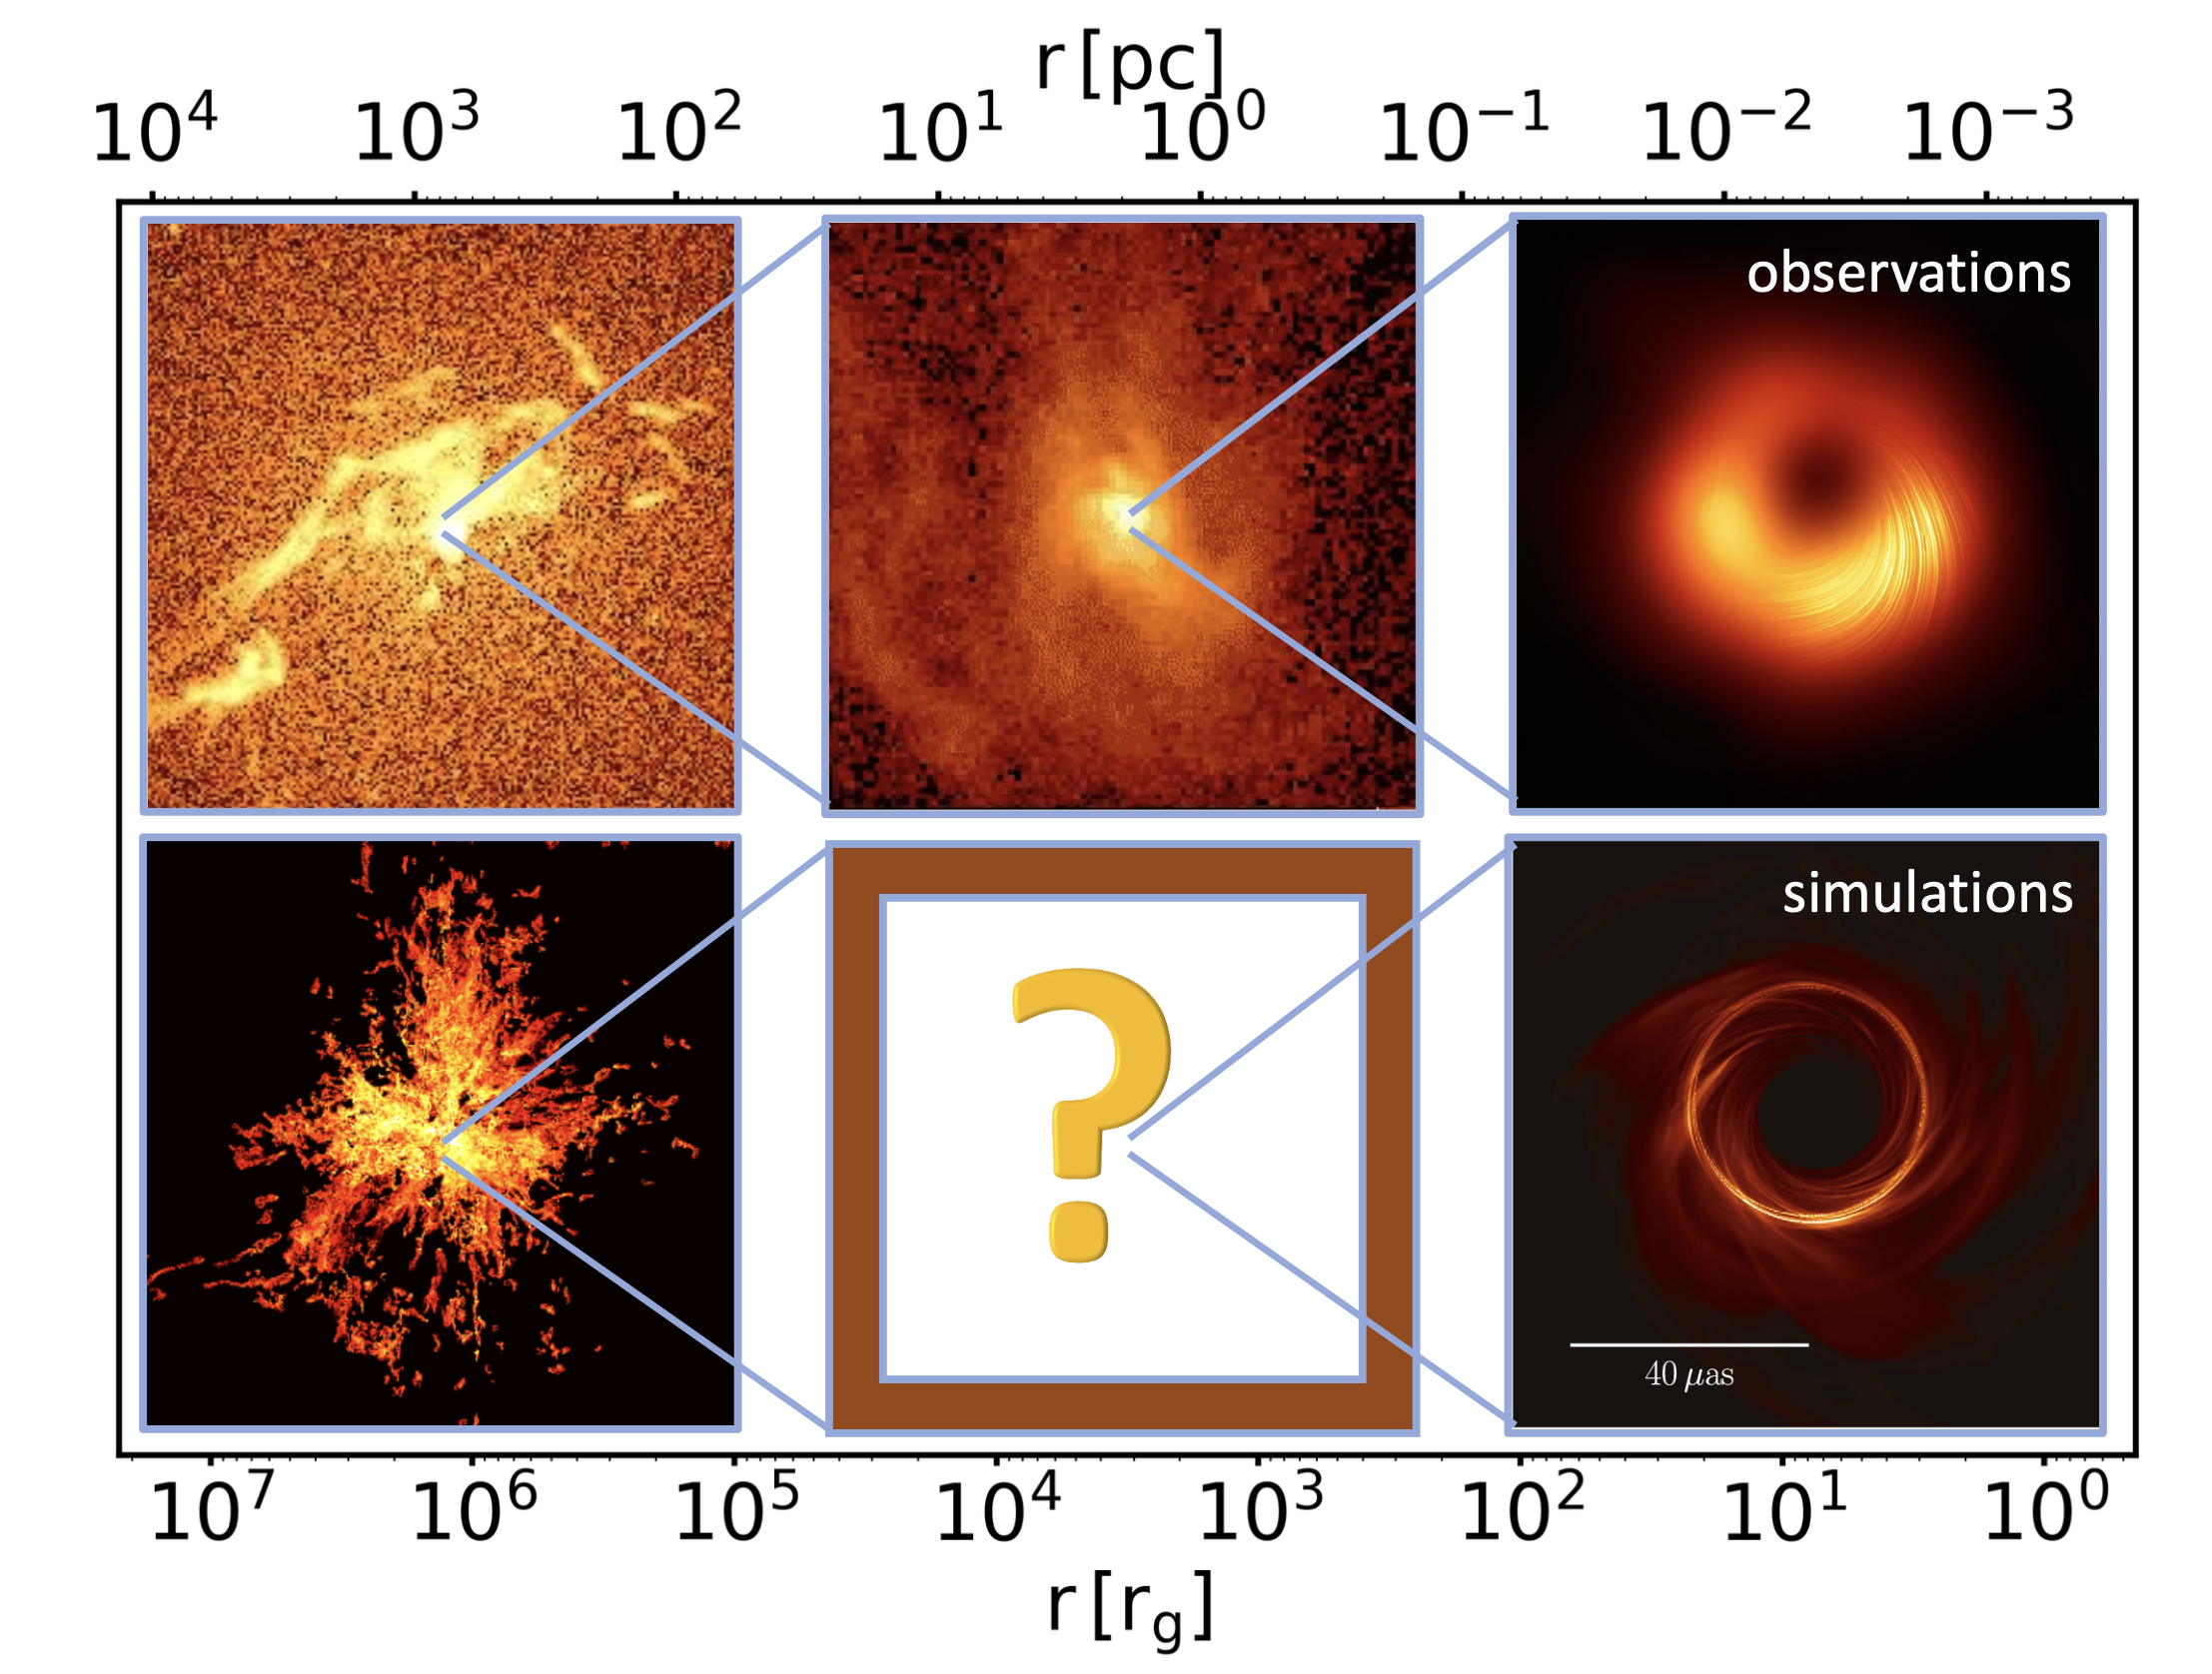
\includegraphics[width=0.8\linewidth]{Sim_img/gap_theory.png}
    \caption{
    Observations of M87 (top panels) from galaxy scale to event-horizon scale (left to right) compared with numerical simulations (bottom panels).
    Top left panel: (MUSE) \halpha+[\ion{N}{2}] image of the central $\sim 10$\,kpc region of M87 \citep{boselli_virgo_2019}.
    Top middle panel: (Hubble) \halpha\ image of the central few hundred pc of M87 \citep{walsh_m87_2013}.
    Top right panel: EHT image of the accretion flow near the SMBH in the center of M87 \citep{eht_one}.
    Bottom left panel: \halpha\ map of the central tens of kpc of a simulated cluster central galaxy \citep{li_cooling_2015}.
    Bottom right panel: GRMHD simulation of the M87 SMBH \citep{eht_one}.
    On the meso-scale, from the Bondi radius (hundreds of pc) to the outer edge of the accretion disk, the observed accretion flow is multiphase and dynamically complex, but theoretical understanding lags behind observations. This chapter addresses this gap and bridges two important scales in SMBH accretion studies. Credit: Yuan Li.}
    \label{fig:theory-gap}
\end{figure}

The following section is adapted from Ha \& Li 2026, manuscript in preparation.

\section{Gas Morphology and Accretion Dynamics of Multiphase Accretion onto SMBHs}

\publicationdetails[From]
{Ha \& Li 2026, manuscript in preparation}
{Trung Ha\footnotemark[1] and Yuan Li\footnotemark[1]}
{Low-luminosity active galactic nuclei regulate the hot atmospheres of massive elliptical galaxies through jet-driven feedback, yet the accretion flow linking kpc-scale cooling to event-horizon-scale black hole feeding remains poorly understood. We study multiphase, multi-scale accretion in elliptical galaxies with a suite of hydrodynamic (HD) simulations. We initialize the galaxy using profiles motivated by \textit{Chandra} observations of M87 and the Virgo cluster, and use nested static mesh refinement (SMR) to follow the gas from the kpc scale down to $\sim 50\,r_{\rm g} \approx 16$\,mpc. We find that AGN jet feedback facilitates the formation of cool gas filaments at the kpc scale. These filaments carry angular momentum and circularize into a disk as the accretion flow is resolved to smaller radii. Outside $\sim 10^3\,r_{\rm g}$, the hot and cool phases are dynamically decoupled: the cool gas primarily forms rotationally supported disks, while the hot gas accretes more radially. Inside this scale, the cool gas is compression-heated to the virial temperature, and the innermost accretion flow becomes dominated by the hot phase. The net inflow rate follows a radial scaling $\dot{M}\propto r^k$, with $0.40 \leq k \leq 0.69$, broadly consistent with previous results for radiatively inefficient accretion flows (RIAFs). We also revisit the Bondi accretion model in this multiphase environment. We find that the Bondi model can estimate the hot gas inflow rate, but does not describe the cool, rotationally supported accretion flow. Our results suggest that unresolved black hole accretion rates in galaxy-scale and cosmological simulations should be estimated from the hot gas inflow outside the cool gas precipitation radius, then scaled inward using the measured accretion-rate relation.}
{\footnotetext[1]{Department of Astronomy, University of Massachusetts Amherst, Amherst, MA 01003, USA}}
\setcounter{footnote}{0}

\subsection{Introduction}
\label{sec:agn-intro}

The centers of most galaxies host supermassive black holes \citep[SMBHs,][]{magorrian_demography_1998,kormendy_coevolution_2013}.
When SMBHs accrete at high rates ($\dot{M} \gtrsim 10^{-3} \dot{M}_{\rm Edd}$, where $\dot{M}_{\rm Edd}$\ is the Eddington accretion rate), their accretion disks are radiatively efficient, and feedback is dominated by radiation pressure associated with the large inflow of matter \citep[e.g.,][]{cielo_agn_2018}. This regime is commonly referred to as \textit{quasar-mode feedback}.
Quasar-mode feedback is important in high-redshift active galactic nuclei \citep[AGNs, e.g.,][]{di_matteo_energy_2005}, but is less commonly seen in the local universe.
At low accretion rates ($\dot{M} \ll \dot{M}_{\rm Edd}$), the accretion disks are radiatively inefficient. Feedback is predominantly mechanical, mediated by relativistic jets that produce radio emission. The regime is thus known as \textit{radio-mode feedback} \citep[][]{mcnamara_heating_2005}.
These systems are typically observed as low-luminosity AGNs and constitute $\approx 99\%$ of the AGN population in the local universe \citep[][]{birchall_incidence_2022}.


Current theory and observations support a picture in which SMBH jet-driven feedback regulates the atmosphere of the host galaxies of low-luminosity AGNs \citep[][]{mcnamara_mechanical_2012}.
In this picture, jets inject energy into the surrounding medium, which suppresses cooling and star formation \citep[][]{combes_agn_2017}.
As cooling slows down, the fuel supply diminishes, jet power declines, and cooling can resume, repeating the cycle.
Many systems, such as M87 and other central galaxies in galaxy clusters and groups, are observed to harbor spatially extended cool clouds \citep[e.g.,][]{edge_detection_2001,salome_cold_2003,simionescu_alma_2018,boselli_virgo_2019}. These cool clouds often appear filamentary on kpc to tens of kpc scales, and exhibit a lack of large-scale coherent motion \citep[e.g.,][]{olivares_ubiquitous_2019}. Numerical simulations show that the cool clouds may have condensed out of the hot atmosphere due to thermal instability \citep{mccourt_thermal_2012,sharma_thermal_2012}, which can be triggered by jet feedback \citep{li_2014a}. The fate of the multiphase gas is unclear. While some observations suggest that the cool clouds may be directly feeding the SMBH as cold clumps \citep[e.g.,][]{tremblay_cold_2016}, recent high-resolution observations suggest that the multiphase gas may settle into a rotating structure at the $\sim100$\,pc scale \citep{osorno_revisiting_2023,oosterloo_closing_2023,tamhane_hst_2026}.


Two main uncertainties in understanding radio-mode SMBH feeding and feedback are the mass accretion rate onto SMBHs, \mdotbh, and the phase of the accretion flow. \mdotbh\ is difficult to measure directly because of the extremely high resolution required.
One common way to estimate the accretion rate is using the classical Bondi-Hoyle-Lyttleton model \citep[hereafter the ``Bondi model'',][]{hoyle_effect_1939,bondi_mechanism_1944,bondi_spherically_1952}.

For M87, gas properties measured near $r_{\rm B}\approx120$\,pc (five orders of magnitude larger than the event horizon of the SMBH) imply a Bondi accretion rate of $\dot{M}_{\rm B} \approx 0.1\, M_{\odot}\, \mathrm{yr}^{-1}$ \citep[][]{di_matteo_accretion_2003, russell_inside_2015}.
However, estimates of \mdotbh\ via other methods, such as AGN luminosity \citep[][]{broderick_event_2015}, Faraday rotation \citep[][]{kuo_measuring_2014}, and Event Horizon Telescope \citep[EHT,][]{eht_eight} observations are at odds with the Bondi estimate, often orders of magnitude smaller than \mdotb.
This discrepancy suggests that the Bondi model's assumptions of spherical accretion and a homogeneous, single-phase medium do not capture the multiphase, turbulent, and rotating accretion flows expected around low-luminosity AGNs.

Despite the Bondi model's overestimation of the true accretion rates in low-luminosity AGNs, many state-of-the-art cosmological simulations still adopt this model or close variants to estimate \mdotbh\ and the associated feedback power \citep[e.g.,][]{schaye_eagle_2015, tremmel_romulus_2017,pillepich_simulating_2018,dave_simba_2019,pakmor_millenniumtng_2023}.
This is largely because their typical resolutions ($\sim 0.1$--$1$\,kpc) cannot resolve the relevant black hole accretion physics.

A multi-scale numerical study that connects the gas at the galaxy-scale to the accretion flow at the event-horizon-scale is needed to provide better subgrid prescriptions of SMBH accretion in cosmological simulations.
Recent efforts have pursued this goal using a range of strategies, including hyper-refinement of selected halos from cosmological simulations \citep[e.g.,][]{angles-alcazar_cosmological_2021,hopkins_forged_2024,kaaz_h-amr_2025}, repeated zoom-ins of individual galaxies \citep[e.g.,][]{ressler_ab_2020,guo_toward_2023,guo_magnetized_2024}, reduced scale separation \citep[e.g.,][]{lalakos_bridging_2022}, and multi-zone or cyclic approaches spanning many length scales \citep[e.g.,][]{yuan_numerical_2012,cho_multizone_2024,guo_cyclic_2025}.

In this work, we study the formation and dynamics of a multiphase accretion flow under the influence of jet feedback in an idealized galaxy based on the nearby radio galaxy M87, the central galaxy of the Virgo cluster.
M87 hosts a SMBH of mass $M_{\rm BH} \approx 6.5\times10^9\,\mathrm{M_{\odot}}$ \citep[][]{eht_six} and has been the focus of extensive multiwavelength observations.
On kiloparsec scales, extended multiphase filaments are observed \citep{boselli_virgo_2019}. On tens-of-parsec scales, a multiphase circumnuclear disk has also been observed \citep{walsh_m87_2013}.
On horizon scales, the EHT has imaged the shadow of M87$^{\star}$ \citep[][]{eht_one}, and recent observations have begun to directly link the inner accretion flow to the emerging jet \citep[][]{lu_ring-like_2023}.
Together, these observations make M87 a prime candidate for testing models of multiphase feeding and jet feedback across vast spatial scales.



Using a suite of hydrodynamic (HD) simulations spanning from galaxy scales to tens of Schwarzschild radii, we study the rate, phase, morphology, and kinematics of the accretion flow.
The paper is organized as follows. In Section~\ref{sec:method}, we describe the numerical methods and physical models used in the galaxy-scale and meso-scale simulations. In Section~\ref{sec:galaxy-scale-result}, we present the galaxy evolution over 2\,Gyr. We discuss the multi-scale accretion dynamics, disk formation, and thermodynamics in Section~\ref{sec:zoom-in-result}. We discuss the Bondi accretion model in the context of a turbulent, multiphase environment, the effects of the size of the accretion zone on the cool phase's filamentary, chaotic accretion, as well as limitations of our simulations in Section~\ref{sec:discussion}. We conclude and summarize our main results in Section~\ref{sec:conclusion}.





\subsection{Methodology} \label{sec:method}

\begin{table}
\centering
\caption{Initial conditions\label{tab:initial-condition}}
\begin{tabular}{lcc}
\hline
\hline
Parameter & Value & Equation \\
\hline
Physical parameters & & \\
$K_0$ & 7 keV\,cm$^2$ & \ref{eq:entropy} \\
$\Gamma$ & 1.1 & \ref{eq:entropy}\\
$x$ & $r/(2\,\rm kpc)$ & \ref{eq:entropy} \\
$n (x=1)$ & 0.1 cm$^{-3}$ & \ref{eq:pressure} \\
$M_{\rm BH}$ & $6.5 \times 10^9 M_{\odot}$ & \ref{eq:gacc} \\
$M_{\rm DM}$ & $3 \times 10^{13} M_{\odot}$ & \ref{eq:gacc} \\
$R_{\rm DM}$ & $60$\,kpc & \ref{eq:gacc}\\
$M_{\star}$ & $3 \times 10^{11} M_{\odot}$ & \ref{eq:gacc} \\
$R_{\star}$ & $2$\,kpc & \ref{eq:gacc} \\
\hline
Simulation parameters & & \\
$L_{\rm box}$ & 128 kpc & \\
$R_{\rm out}$ & 64 kpc & \\
$n (r<R_{\rm acc})$ & $5 \times 10^{-3}$\,cm$^{-3}$ & \\
$T_{\rm floor}$ & $2\times10^5$\,K & \\
$n_{\rm floor}$ & $10^{-3}$\,cm$^{-3}$ & \\
$v_{\rm jet}$ & 3000 km\,s$^{-1}$ & \ref{eq:jet-momentum} \\
\hline
\end{tabular}
\parbox{0.6\linewidth}{\footnotesize \textit{Note.} The ``Equation'' column denotes the first instance in which the parameter is referenced.}
\end{table}



We carry out three-dimensional (3D) HD simulations using the \ath\ code \citep{stone_athena_2020}.
\ath~is a grid-based numerical code for astrophysical fluid dynamics simulations.

We solve the hydrodynamic equations using the Harten--Lax--van Leer--Contact Riemann solver, a piecewise linear reconstruction method, and a second-order Runge-Kutta time integrator.


Overall, the code solves the following HD equations:
\begin{equation}
    \frac{\partial \rho}{\partial t} + \nabla \cdot (\rho \mathbf{v}) = 0,
\end{equation}
\begin{equation}
    \frac{\partial \rho \mathbf{v}}{\partial t} + \nabla \cdot (P \mathbf{I} + \rho \mathbf{v} \mathbf{v}) = \rho \mathbf{g},
\end{equation}
\begin{equation}
    \frac{\partial E}{\partial t} + \nabla \cdot [(E+P)\mathbf{v}] = \rho \mathbf{g} \cdot \mathbf{v} - Q_{-},
\end{equation}
which are the continuity equation, the momentum conservation equation, and the energy conservation equation, respectively.
$Q_{-}$\ is the heat loss per unit volume due to radiative cooling.
We do not include any explicit heating term in our simulations, but heat can be generated through numerical dissipation of shocks and turbulence.


\subsubsection{Initial conditions} \label{subsec:init}

Our galaxy-scale simulations use a hydrostatic equilibrium initial condition based on the observations of the Virgo cluster \citep{urban_x-ray_2011} and of its central galaxy M87 \citep{russell_inside_2015}.
We start with a flat core entropy profile following \citet{martizzi_simulations_2019}:
\begin{equation}
\label{eq:entropy}
    K_{\rm gas}(x) = \frac{K_0}{2}(1+x^{\Gamma}),
\end{equation}
where $K_{0}=7$~keV cm$^2$, $\Gamma = 1.1$, and $x \equiv r/(2~\mathrm{kpc})$~is the dimensionless length scale of the system \citep{urban_x-ray_2011}.
The pressure is a function of the entropy and the gas number density:
\begin{equation}
\label{eq:pressure}
    P(x) = K_{\rm gas}(x) \cdot n(x)^{\gamma},
\end{equation}
where $\gamma = 5/3$ is the adiabatic gas index.

Assuming hydrostatic equilibrium:
\begin{equation}
    \frac{dP(r)}{dr} + \rho g = 0\, ,
\end{equation}
we have
\begin{equation}
\label{eq:dn_dx}
    \frac{dn}{dx} = \frac{2 (r_0 / K_0) \mu m_{\rm H} n(x)^{2-\gamma} \cdot g - \Gamma n(x) \cdot x^{\Gamma - 1} }{1+x^{\Gamma}\gamma},
\end{equation}
where $n$ is the number density, $\mu \approx 0.6$\ is the mean molecular weight, and $m_{\rm H}$\ is the hydrogen mass.
Using the observed density $n(x=1)=0.1\,\mathrm{cm}^{-3}$ \citep{russell_inside_2015}, we numerically solve Equation~\ref{eq:dn_dx} for $n(x)$ using a fourth-order Runge-Kutta scheme.
At time $t= 0$, we verify that the density and temperature profiles closely match the observed profiles (see Figure~\ref{fig:r-prof-meso}).

We inject a small density perturbation on the order of a few percent ($\sim 5\%$) on top of the hydrostatic equilibrium solution, using a Gaussian noise distribution, to seed initial instability.
A summary of the physical parameters, as well as the global simulation parameters, is listed in Table~\ref{tab:initial-condition}.

\begin{table}
\centering
\caption{Simulations and parameters\label{tab:simulations}}
\begin{tabular}{lccccc}
\hline
\hline
Name & \racc\ (mpc) [($r_{\rm g}$)] & $N_{\rm refine}$ & $t_{\rm start}$ (Myr) & $\Delta t$ (Myr) \\
(1) & (2) & (3) & (4) & (5) \\
\hline
Galaxy-scale \\
R8 & $4^8$ [$2.1 \times 10^5$] & 8 & 0 & 2000 \\
\hline
Zoom-in \\
R10 & $4^7$ [$5.3 \times 10^4$] & 10 & 920 & 50 \\
R12 & $4^6$ [$1.3 \times 10^4$] & 12 & 925 & 5 \\
R14 & $4^5$ [$3.3 \times 10^3$] & 14 & 928 & 2 \\
R16 & $4^4$ [$8.2 \times 10^2$] & 16 & 929.25 & 0.5 \\
R18 & $4^3$ [$2.1 \times 10^2$] & 18 & 929.55 & 0.05 \\
\hline
Meso-scale \\
R20 & $4^2$ [$5.1 \times 10^1$] & 20 & 929.57 & 0.003 \\
\hline
\end{tabular}

\vspace{0.5em}
\parbox{0.75\columnwidth}{\small\textit{Note.} The galaxy-scale simulation is run first, then snapshots of interest are selected for resimulation with additional nested refinement. The columns list, from left to right: (1) name of the simulation, (2) radius of the accretion zone, (3) number of nested refinement levels, (4) start time of the simulation, (5) duration of the simulation.}
\end{table}


\subsubsection{Galaxy-scale simulation setup} \label{subsec:setup}

Our simulations use Cartesian grids.
The root grid consists of $128^3$ cells with a domain width of $L_{\rm box} = 128$\,kpc.
This translates to a root resolution of $\Delta x_{\rm max} = 1$\,kpc.
At each refinement level $\ell$, the center 64 cells per dimension of level $\ell-1$\ are replaced by twice as many cells with half the width, reaching a spatial resolution of  $\Delta x_{\rm min} = 1/2^{\ell}$\,kpc.
We apply 8 levels of nested static mesh refinement (SMR) to our galaxy-scale simulation, which allows us to resolve the accretion flows down to $\Delta x_{\rm min,R8}\approx 4$\,pc at the center of the domain.

We perform several galaxy-scale simulations with varying jet parameters, such as the jet kinetic fraction ($f_{\rm kin}$), the height and width of the jet base (see Section~\ref{subsubsec:jet}). Each is evolved for 1 Gyr, except for the fiducial run which is evolved for 2 Gyr.
We mainly focus on the results from the fiducial run, R8, in this paper.

A spherically symmetric outer boundary condition is implemented at $R_{\rm out} = 64$\,kpc, where primitive variables ($\rho,\ p,\ \mathbf{v}$) are reset to an initial hydrostatic equilibrium solution at each time step.
An inner boundary of a spherical accretion (sink) region is set up near the center of the domain at $R_{\rm acc,R8} = 4^8\,\mathrm{mpc}\approx 65.5$\,pc initially. We gradually shrink this boundary for the meso-scale simulations, described in \fullsectionref{subsec:meso}.
This region acts like a ``vacuum'' zone, where the density is reset at every step to $n_{r < R_{\rm acc}} = 5\times 10^{-3}~\mathrm{cm^{-3}}$ and the temperature is reset to the global floor temperature $T_{r < R_{\rm acc}} = T_{\rm floor}$.
This inner boundary accretion region can prevent unrealistic pressure bounces as gas builds up in the center of the domain, following a numerical treatment similar to \citet{guo_toward_2023}. We also track the accretion rate through this boundary as a proxy for the black hole accretion rate.

The galaxy-scale simulations include several physical processes important in regulating the feeding--feedback balance in M87: static gravitational potential, radiative cooling, and AGN jet feedback.
Below, we discuss our implementation of each process in more detail.

\centerline{\textbf{Static gravitational potential}} \label{subsubsec:grav}


We model the SMBH as a point mass with $M_{\rm BH} = 6.5 \times 10^9~M_{\odot}$ \citep[e.g.,][]{eht_six}, and we model both the dark matter halo and the stars as Navarro-Frenk-White (NFW) profiles \citep{navarro_structure_1996}.
The mass enclosed at a given distance $r$ from the SMBH is:
\begin{equation}
\label{eq:mass}
    M(r) = M_0 \left[\ln(1 + \frac{r}{r_0}) - \frac{r}{r + r_0}\right],
\end{equation}
where $M_0 = 3\times10^{13} M_{\odot}$ and $r_0 = 60$~kpc for the dark matter halo, and $M_0 = 3\times10^{11} M_{\odot}$ and $r_0 = 2$~kpc for the stars.
These parameters are chosen such that the mass profiles match the observed profiles in \citet{gebhardt_black_2009}.

The gravitational acceleration as a function of distance from the SMBH is then:
\begin{equation}
\label{eq:gacc}
    \mathbf{g}(r) = - \frac{G(M_{\rm BH} + M_{\rm DM}(r) + M_{\star}(r))}{r^2} \hat{\mathbf{r}}.
\end{equation}
Inside the accretion zone, we multiply $\mathbf{g}(r)$\ by a softening factor, $F_s$, to prevent fast-moving accreted gas from escaping the sink before it is removed,
following \citet{guo_toward_2023}:
\begin{equation}
    F_s|_{r < R_{\rm acc}} = \frac{r^3 (1-e^{-r^{2}/r_{a}^2})}{(r^2 + r_{a}^2 \cdot e^{-r^{2}/r_{a}^2})^{3/2}},
\end{equation}
where $r_{a} = R_{\rm acc}/2$.

\centerline{\textbf{Radiative cooling}}

We model radiative cooling as a source term in the simulation:
\begin{equation}
    Q_{-} = n^2\Lambda(T),
\end{equation}
where $n$ is the number density in cm$^{-3}$, and $\Lambda(T)$ is the cooling function in erg s$^{-1}$~cm$^3$, modeled as a piecewise function of the temperature, assuming solar metallicity.

At $\log T > 8.15$,
\begin{equation}
    \Lambda(T) = 10^{-26.065}T^{0.45},
\end{equation}
following \citet{schneider_introducing_2018}.
For $\log T \leq 8.15$, we interpolate to obtain $\Lambda(T)$~from a tabulated emissivity curve following Table 2 of \citet{schure_new_2009}.

In most of our simulations, we force a temperature floor at $T_{\rm floor}=2\times10^5$\,K, but in several short-term runs, we set the temperature floor to $10^4$\,K (see Section~\ref{subsec:limitations}).
A global number density floor is also applied at $n_{\rm floor} =10^{-3}\,\mathrm{cm^{-3}}$.
Throughout this paper, we refer to gas at temperatures below and above $10^6$\,K as the cool and hot phases, respectively.

\centerline{\textbf{Black hole accretion and AGN jet feedback}}
\label{subsubsec:jet}

We compute the black hole accretion rate by measuring the accretion rate at the inner boundary of the simulation, then scaling the value as follows:
\begin{equation}
\label{eq:scaling}
    \dot{M}_{\rm BH} = \dot{M}_{|R_{\rm acc}} \cdot \left(\frac{100\,r_{\rm g}}{R_{\rm acc}}\right)^{1/2},
\end{equation}
where $\dot{M}_{|R_{\rm acc}}$\ is the accretion rate through the accretion zone, \racc\ is the radius of the accretion zone, and $r_{\rm g}$\ is the gravitational radius of the black hole.

We adopt $k=1/2$ as a calibration choice following previous numerical studies of low-luminosity AGNs \citep[e.g.,][]{yuan_numerical_2012, guo_magnetized_2024}, but use a different normalization based on the accretion behavior of our own meso-scale simulations.
More specifically, we observe that the accretion rate profile flattens inside 100\,\rg\ such that $\dot{M}_{r<100\,r_{\rm g}} \approx \dot{M}_{r = 100\,r_{\rm g}}$, so the factor of $100\,r_{\rm g}$\ was added to account for the break in the scaling relation.
In runs where \racc $< 100\,r_{\rm g}$, we measure the accretion rate through the inner boundary without applying a correction.

In our simulations, AGN feedback is modeled with a pair of bipolar jets, loosely following the AGN feedback scheme described in \citet{li_2014a,li_2014b}. The jet power $\mathcal{P}_{\rm jet}$\ is computed based on the accretion rate through the sink region:
\begin{equation} \label{eq:jet_power}
    \mathcal{P}_{\rm jet} = \eta \dot{M}_{\rm acc} c^2,
\end{equation}
where $\eta$\ is the effective feedback efficiency of the SMBH\@.
Every 5 Myr, the mass accretion rate over this period is calculated and then averaged over time to obtain the jet power over the next 5 Myr.
Jet material is injected along two ends of a cylinder centered on the SMBH, such that each side contains a circular layer of cells at height $H_{\rm jet} = 20\,R_{\rm acc} \approx 1.3$\,kpc and radius $R_{\rm jet} = 2\,R_{\rm acc} \approx 130$\,pc.
We also ran simulations with the jet base height at $H_{\rm jet} = 10\,R_{\rm acc} \approx 650$\,pc and a radius of $R_{\rm jet} = R_{\rm acc} \approx 65$\,pc. We found that while the exact radius of the base does not significantly affect the cool gas morphology, a base height of $H_{\rm jet} =20\,R_{\rm acc}$ produces cool gas filaments at the kpc scale in better agreement with observations than the alternative.
The direction of momentum injection is held fixed at a zenith angle $\theta =15$\textdegree~with respect to the $z$-axis, while the azimuth angle ($\phi$) is reset randomly every 10 Myr to mimic jet precession.
In successive zoom-ins (see Table~\ref{tab:simulations} and \fullsectionref{subsec:meso}), we dynamically scale the jet base height and radius such that they remain the same multiples of \racc, up to the third zoom-in simulation, R14.

We solve the equations of momentum and energy conservation to compute the amount of momentum and energy injected into each cell. The injected density per cell per time step is given by:
\begin{equation}
\label{eq:drho}
    \Delta \rho = \frac{\dot{M}_{\rm acc} W_{\rm g} dt}{2V_{\rm jet}},
\end{equation}
where $V_{\rm jet}$\ is the volume of one jet base, and $W_{\rm g}$\ is a Gaussian weight based on how far away from the $z$-axis the cell is. The momentum density vector is updated accordingly:
\begin{equation}
\label{eq:jet-momentum}
    \Delta p_i = \Delta \rho \cdot v_{i, \rm jet},
\end{equation}
where $i = \{x,y,z\}$ and $v_{i,\rm jet}$ is calculated based on the angle of precession. We set the jet velocity $|v_{\rm jet}| = 3000\,\mathrm{km~s}^{-1} \approx 1\%\,c$\ for all simulations.
The kinetic energy density injected is inferred from the density:
\begin{equation}
\label{eq:jet-KE}
    \Delta \mathcal{E}_{\rm kin} = \frac{1}{2} \Delta \rho v_{\rm jet}^2.
\end{equation}
We control the amount of energy injected in the form of kinetic vs.\ thermal energy using a kinetic jet fraction parameter $f_{\rm kin} = \Delta \mathcal{E}_{\rm kin} / \Delta \mathcal{E}_{\rm tot}$. In our set of fiducial simulations, we choose \fkin\ $=0.8$. We varied \fkin\ between $0.7$ and $1$ in test runs, and found that the choice of $0.8$ results in cool gas formation that is most consistent with observations.

The jet feedback efficiency is calculated as:

\begin{equation} \label{eq:jet_eff}
    \frac{v_{\rm jet}^2}{2f_{\rm kin} c^2} = \eta.
\end{equation}
For our choice of $v_{\rm jet}$\ and \fkin, $\eta \sim 10^{-4}$, which is in the typical range of efficiencies used in numerical studies of AGN feedback \citep[e.g.,][]{li_2014a, li_2014b, prasad_cool_2015, yang_how_2016}.


\subsubsection{Meso-scale simulation setup} \fullsubsubsectionlabel{subsec:meso}

We perform a set of meso-scale simulations to follow the accretion flow from the galaxy scale to near the event horizon of M87$^{\star}$. We first perform the galaxy-scale simulations described in Section~\ref{subsec:setup}.
We then identify three snapshots of interest for meso-scale resimulation, at times $t = 920\,$Myr, $1440\,$Myr, and $1500$\,Myr.
In the next sections, we present results from the first zoom-in simulation at $t_{\rm start} = 920$\,Myr, but note that the conclusions are generally consistent across all three simulations.


At the beginning of each re-simulation, the galaxy-scale simulation (R8) is refined by two additional levels of SMR, and the radius of the accretion zone, \racc, is shrunk by a factor of four. This zoom-in is then evolved for $\Delta t \geq 10^3\,t_{\rm ff}$, where $t_{\rm ff}$\ is the free-fall time of the gas measured at the new inner boundary. Successive zoom-ins are also performed following the same procedure until we reach
20 levels of SMR (R20, or the ``meso-scale simulation''), for a maximum resolution of $\Delta x_{\rm min,R20} \approx 10^{-3}$\,pc, or $\approx 3\, r_{\rm g}$ for M87\@.
The smallest accretion region has a radius $R_{\rm acc,R20} = 4^2\,\mathrm{mpc} \approx 50\, r_{\rm g}$ (see Table~\ref{tab:simulations} for a detailed description of each zoom-in).

We evolve the meso-scale simulations for 3 kyr. During their evolution, all physical processes from the galaxy-scale simulation are retained. One exception is the jet feedback, which is turned off above 14 levels of refinement to save computational time.
We do not expect this choice to significantly alter the meso-scale dynamics.
The jets are very narrow at small scales \citep[][]{asada_structure_2012}, and thus have a limited impact on their immediate surroundings.
On larger (galaxy) scales, jets strongly affect the kinematics of the gas, but the gas infalling from the galaxy-scale does not have enough time to reach the center during the 3\,kyr evolution of the meso-scale simulation.
The typical radial inflow velocity of hot gas is a few hundred $\mathrm{km\,s^{-1}} \approx 0.1--1\,\mathrm{kpc\,Myr^{-1}}$, and is much slower for the cool gas ($\sim 10\,\mathrm{km\,s^{-1}}$).


\begin{figure}[t!]
    \centering
    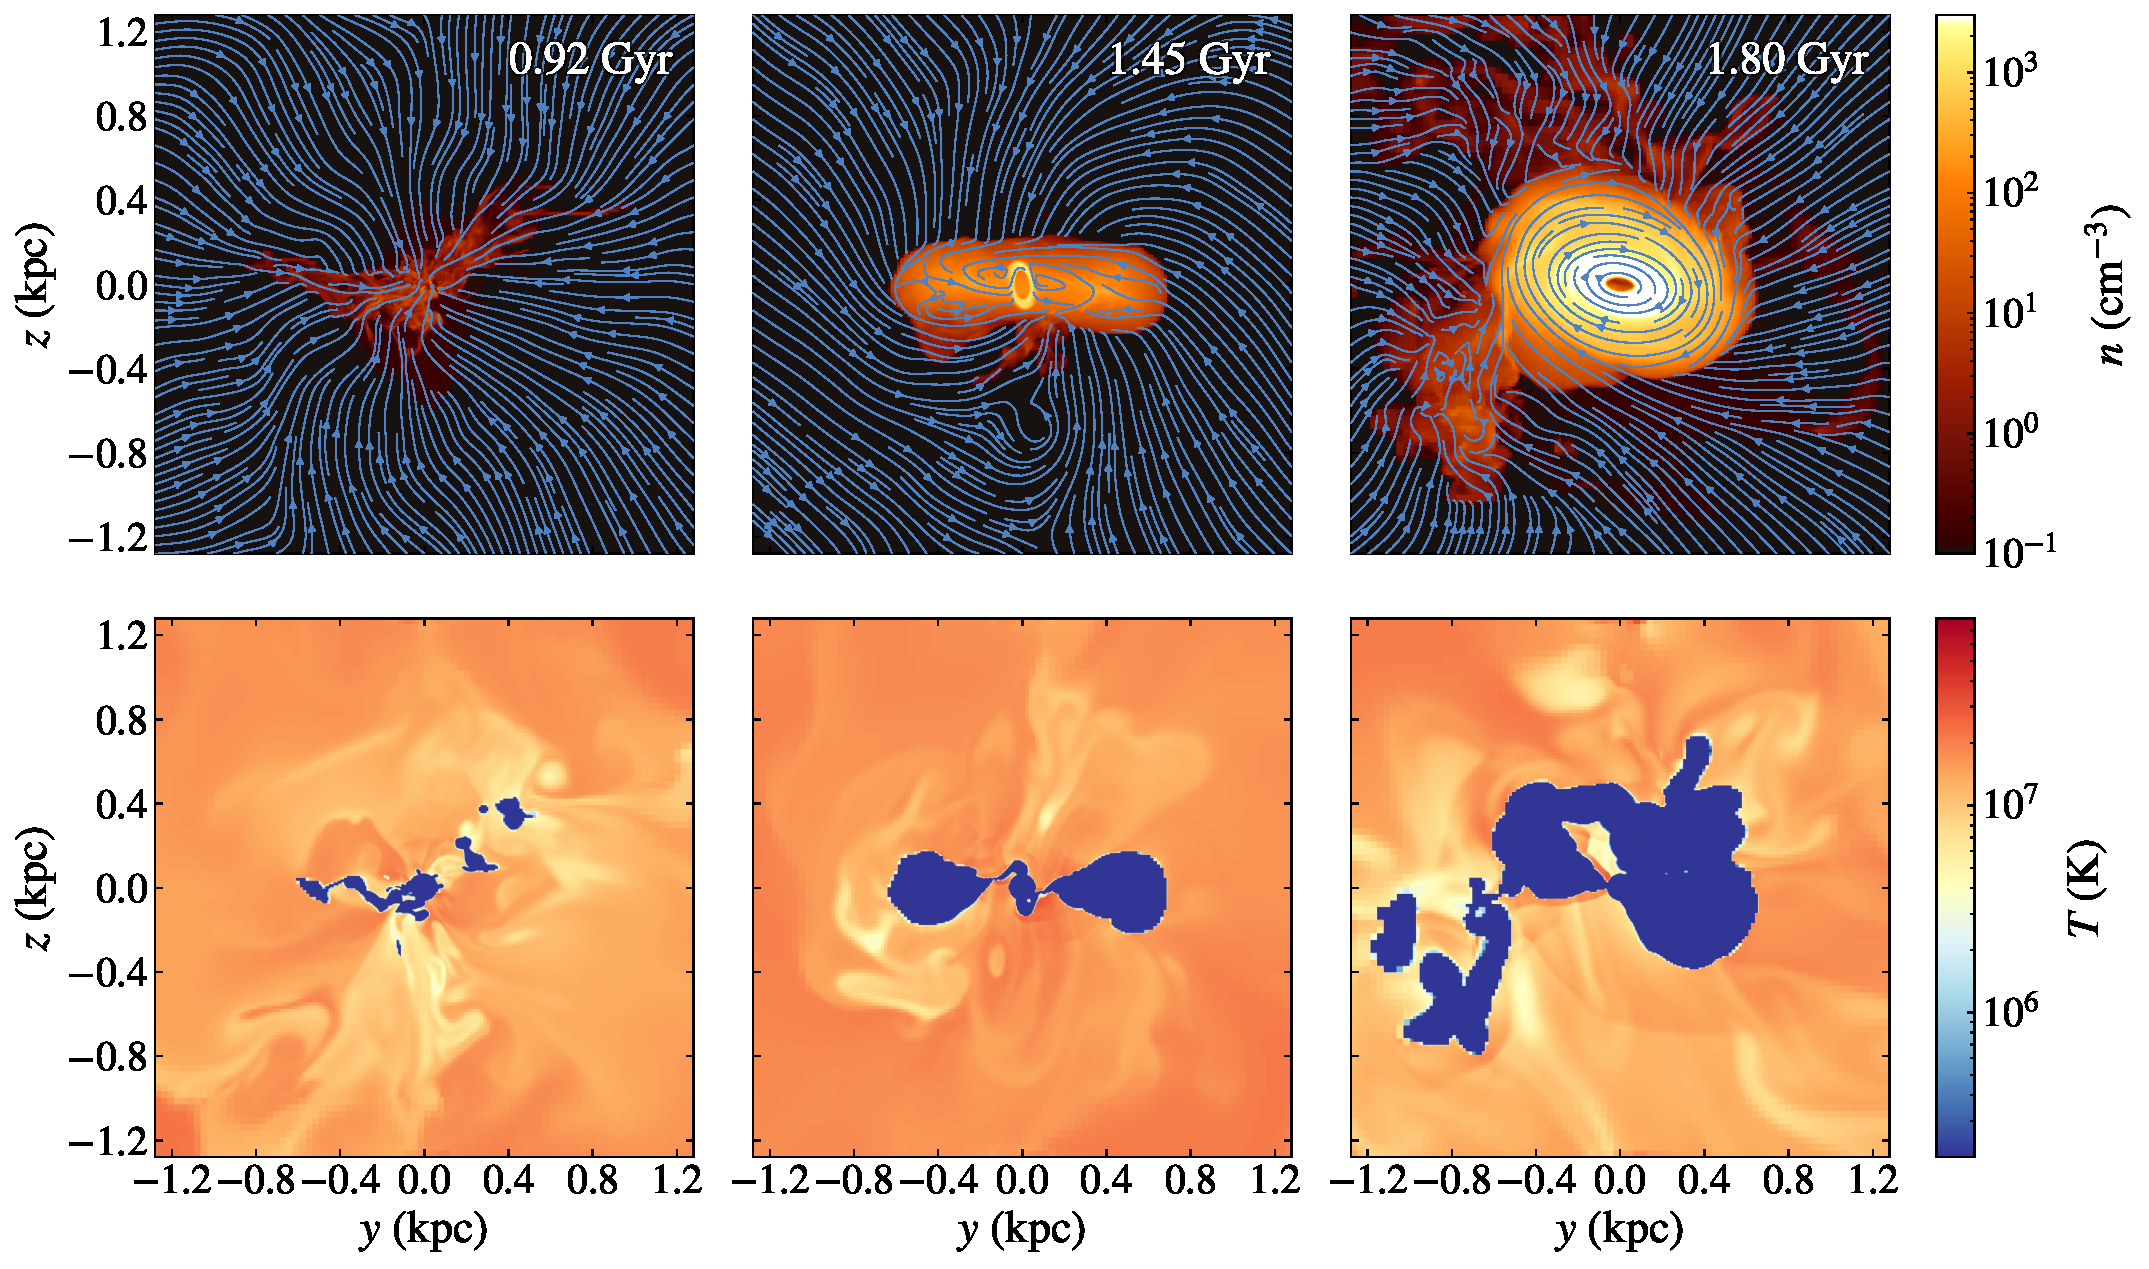
\includegraphics[width=\linewidth]{Sim_img/evolution_disk.pdf}
    \caption{Top: projections along the $x$-axis of the number density, $n$, at three timestamps: $t=920$\,Myr, $t=1450$\,Myr, and $t=1800$\,Myr. Blue streamlines denote the direction of gas flow. Bottom: $yz$-slices of temperature, $T$, at the same timestamps. At the sub-kpc scale, cool gas inflow transitions from filamentary to disky after $\sim 1$\,Gyr.\label{fig:thermodynamics}}
\end{figure}

\subsection{Multiphase gas evolution at the galaxy-scale}
\label{sec:galaxy-scale-result}

\subsubsection{The evolution of cool gas}

Throughout the 2\,Gyr evolution of the galaxy-scale simulation, cool gas precipitates from the hot halo through feedback-assisted thermal instability.
At times $t \lesssim 1$\,Gyr, the cool gas shows filamentary morphology, primarily oriented in the radial direction.
The cool gas cannot sustain ordered rotation because it does not carry enough angular momentum to allow circularization at the size of the accretion zone (see Section~\ref{subsec:filaments} for detailed discussion).
The left panels of Figure~\ref{fig:thermodynamics} show an instance of such a filamentary cool gas structure at time $t = 920\,$Myr.

After 1\,Gyr, the cool gas begins to carry enough angular momentum such that the gas circularizes around the accretion zone, creating a large-scale disk with a diameter reaching $\sim 1\,$kpc.
This disky phase is stable over time, but the disk itself precesses and becomes denser at the core ($n \sim 10^3$--$10^4\,\mathrm{cm^{-3}}$) over time, as can be seen in the middle and right panels of Figure~\ref{fig:thermodynamics}.
We also observe distinct layers of the disk rotating in different (sometimes opposite) directions at various points during this disky phase. The transition from an early filamentary cool structure to a cool disk at $\sim 1$\,Gyr is commonly seen in the jet-feedback simulations of \citet{li_2014a} and \citet{wang_agn_2019}.


\subsubsection{The hot gas}

Throughout the duration of the galaxy-scale simulation, hot gas exists in a quasi-steady state.
The hot gas thermodynamic profiles ($T$, $n$, and $P$) remain consistent with their initial profiles for most of the 2 Gyr evolution (see Figure~\ref{fig:r-prof-meso}).
The average luminosity of the jet is $L \equiv \dot{E}_{\rm jet} \approx 5 \times 10^{41}\, \mathrm{erg\,s^{-1}}$, which is comparable to the \textit{Chandra} X-ray luminosity of the central $\sim 10$\,kpc, but is several times smaller than the cooling luminosity of the entire galaxy.
This value is also in line with measurements of the jet power obtained from M87's multiwavelength spectral energy distribution \citep[SED,][]{prieto_central_2016}, but is one to two orders of magnitude lower than other estimates using X-ray cavity power \citep[e.g.,][]{forman_reflections_2005,russell_radiative_2013} or internal pressure exerted by knots in the jet \citep[e.g.,][]{owen_m87_2000,stawarz_dynamics_2006}.

The hot gas accretes primarily radially onto the inner boundary, with a very small rotational component ($v_{\rm r} \gtrsim 10^3\,v_{\rm rot}$, see also the velocity streamlines in Figure~\ref{fig:thermodynamics}).
The hot gas inflow rate through the inner boundary, $R_{\rm acc,R8} \approx 65$\,pc, is significantly smaller than the cool-gas inflow rate ($\dot{M}_{\rm in,cool} \gtrsim 10\,\dot{M}_{\rm in,hot}$) throughout the 2 Gyr evolution of the galaxy-scale simulation.


\begin{figure}
    \centering
    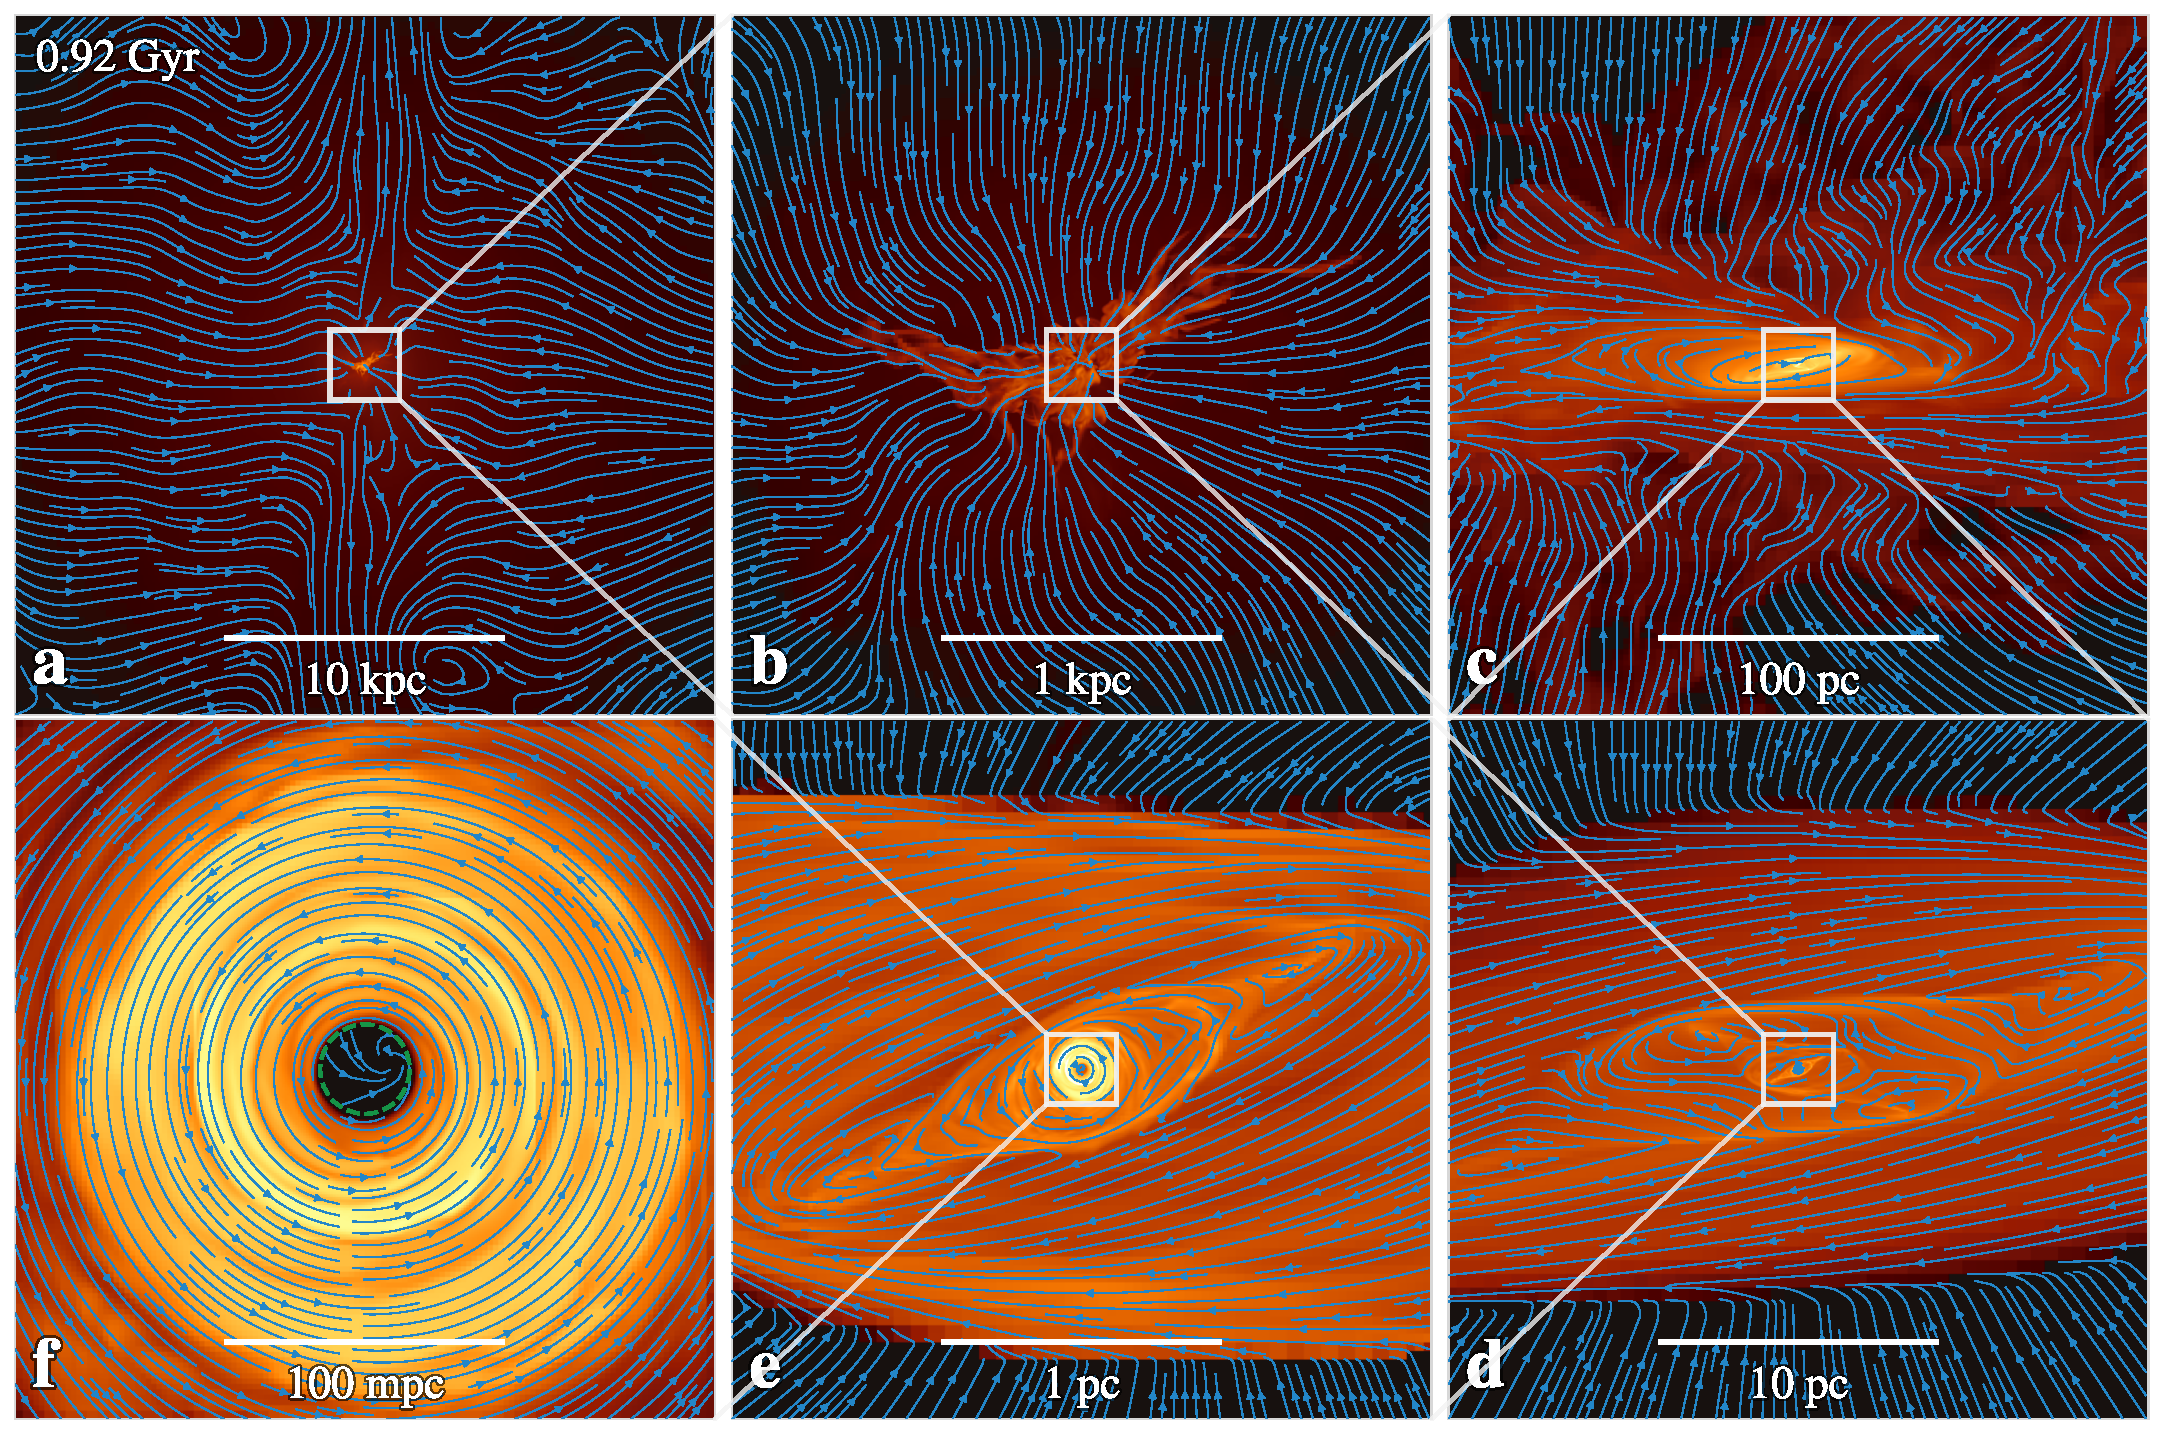
\includegraphics[width=\linewidth]{Sim_img/density_zoom_920Myr.pdf}
    \caption{Projections along the $x$-axis of the density at time $t\approx 920\,$Myr. Each panel is a $10\times$\ zoom of the previous panel, showing the cool gas morphology at various scales. Blue streamlines denote the direction of gas flow, while the green dashed circle in panel (f) denotes the extent of the accretion zone. The color scales are logarithmic, and are dynamically adapted to show features at each scale. At the largest scale, $10^{-2}\,\mathrm{cm^{-3}} < n < 10^2\,\mathrm{cm^{-3}}$. At the smallest scale, $10^{6}\,\mathrm{cm^{-3}} < n < 10^8\,\mathrm{cm^{-3}}$. \label{fig:zoom-in-proj}}
\end{figure}

\subsection{The meso-scale gas dynamics}
\label{sec:zoom-in-result}

We run a series of six zoom-in simulations starting from a galaxy-scale
snapshot to study the meso-scale gas dynamics. In this section, we describe the multiphase gas morphology, thermodynamics, and inflow/outflow rates. The results shown here are from our fiducial zoom-in at $t_{\rm restart} = 920\,$Myr.

\subsubsection{The multi-scale morphology of the cool gas}

Regardless of the galaxy-scale structure, the sub-100-pc cool gas exists within a coherent flow, taking the form of a disk (Figure~\ref{fig:zoom-in-proj}c-f).
The gas circularizes into a disk at a distance:
\begin{equation}
    r_{\rm circ} = \frac{\ell^2}{GM_{\rm BH}},
\end{equation}
where $\ell$\ is the specific angular momentum.
As the accretion zone is resolved at increasingly smaller scales ($R_{\rm acc,R8} \approx 4 \times 10^{3} R_{\rm acc,R20}$), the cool gas is much more likely to have $r_{\rm circ} > R_{\rm acc}$, making meso-scale cool disk formation highly probable. We discuss the effects of the accretion zone size on disk formation and stability in Section~\ref{subsec:filaments}.

The meso-scale disk exhibits dynamic structure across multiple spatial and temporal scales, with distinct gas layers oriented at different angles that continuously evolve as material accretes. Figure~\ref{fig:zoom-in-proj} shows an example snapshot of this multi-layered structure.
At the $\sim 100$\,pc scale, the outer disk is only starting to form from infalling kpc-scale filaments (Figure~\ref{fig:zoom-in-proj}c).
Inside this distance, the disk is thin and warped, and precesses around the $z$-axis.
The warped disk morphology extends two orders of magnitude in scale, from $\sim 50\,$pc to $\sim 0.5\,$pc (Figure~\ref{fig:zoom-in-proj}d-e).
Finally, the cool gas flow transitions to a face-on disk inside $\sim 0.5\,\mathrm{pc} \approx 10^3$\,\rg\ when viewed along the $x$-axis (Figure~\ref{fig:zoom-in-proj}f).

\begin{figure}
    \centering
    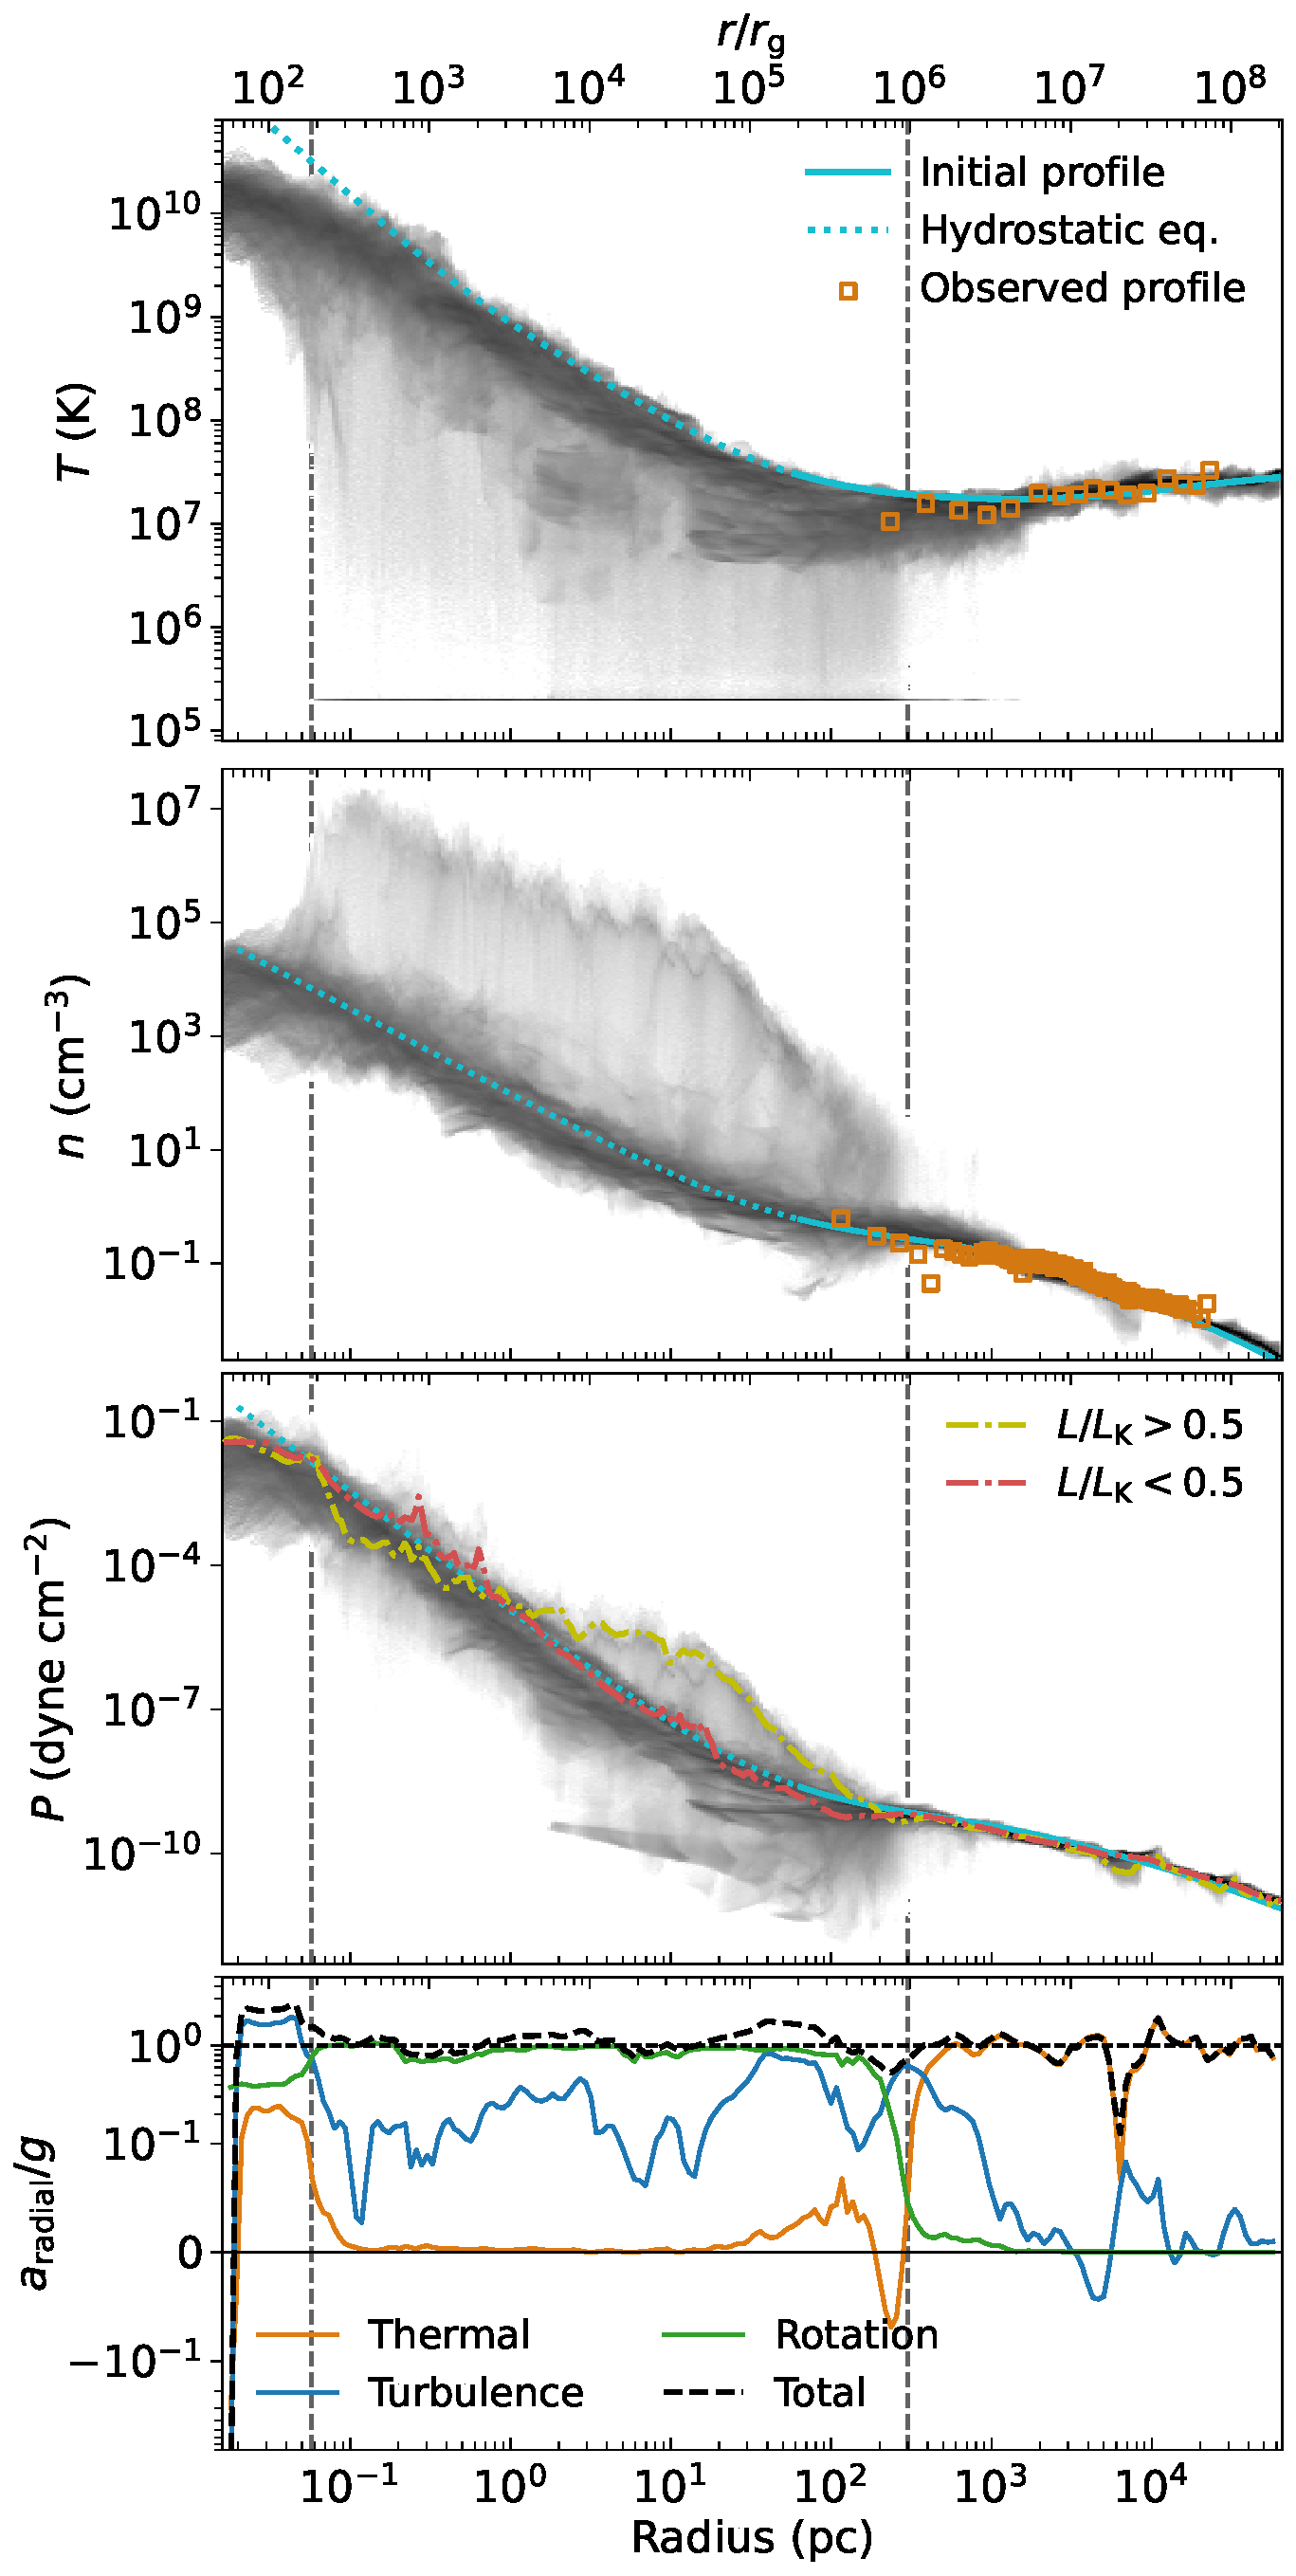
\includegraphics[height=0.65\textheight,keepaspectratio]{Sim_img/thermodynamics.pdf}
    \caption{Top three panels: temperature, number density, and pressure distributions, normalized at each radial bin, for the R20 simulation at $t\approx930\,$ Myr. Orange squares trace Chandra observations of M87, adapted from \citet{russell_inside_2015}. Solid teal lines are the initial profiles, and dotted teal lines are the extended profiles assuming hydrostatic equilibrium where $n(r = 2\,\mathrm{kpc}) = 0.1 \,\mathrm{cm}^{-3}$. The red and yellow lines in the pressure plot trace the mass-weighted profiles of the radially-dominated ($L/L_{\rm K} < 0.5$) and rotationally-dominated ($L/L_{\rm K} > 0.5$) gas, respectively.
    Bottom panel: radial acceleration from thermal pressure, turbulence pressure, and rotation, normalized by gravity, following the framework detailed in \citet{lochhaas_figuring_2022}. Positive values denote radially outward forces (against gravity). A total value of 1 signals radial force balance. The two vertical lines at $r=5.7\times10^{-2}$\,pc and $r=3\times10^{2}$\,pc mark the length scales where cool gas is rotationally supported within cool disks.\label{fig:r-prof-meso}}
\end{figure}

\subsubsection{The thermodynamics of the multiphase gas}

The bulk of the multiphase gas remains close to radial force balance after $\sim 1$\,Gyr.
Although a dense cool component precipitates out of the hot halo, the temperature ($T$), density ($n$), and pressure ($P$) profiles of the hot phase closely follow the initial hydrostatic solution, as obtained from the equations in Section~\ref{subsec:init}, over most scales (see Figure~\ref{fig:r-prof-meso}).
Since the volume-filling hot gas moves primarily in the radial direction, while the cool gas is rotationally supported, we separate the two types of motion by an angular momentum threshold, $L/L_{\rm K} = 0.5$ (where $L_{\rm K}$ is the Keplerian angular momentum) and compute the mass-weighted pressure profile of each type.
The radially-dominated gas practically overlaps with the initial hydrostatic equilibrium solution, while the rotationally-dominated gas deviates significantly from the hydrostatic equilibrium solution at length scales where cool gas is found (third panel of Figure~\ref{fig:r-prof-meso}).


The cool gas acts as an additional component embedded within the mostly hydrostatic hot atmosphere.
Its characteristic density is much higher than that of the hot gas at the same radii, but the maximum value is controlled by the imposed temperature floor, roughly following $n_{\rm cool} \sim \frac{P_{\rm hot}}{k_{\rm B}T_{\rm floor}}$.
A large fraction of the cool gas is at the floor temperature, $T =2\times10^5\,K$, with a smaller fraction ($\sim 40\%$) spanning intermediate temperatures $2\times10^5\,K < T < 10^7\,K$ as it mixes with the hot phase.


To understand the gas's radial force balance across scales and the physical processes responsible for supporting the galaxy against gravitational collapse, we adopt a procedure similar to \citet{lochhaas_figuring_2022} to compute the relative contribution of the different forces acting on the multiphase gas.
Briefly, we consider four support terms: thermal pressure, turbulent pressure, ram pressure, and rotation.
For each component, we compute the radial acceleration it provides against $\mathbf{g}$ and plot these values in the bottom panel of Figure~\ref{fig:r-prof-meso}:
\begin{equation}
\frac{F_{\rm total}}{m_{\rm gas}}
=
-\frac{1}{\rho}\frac{dP_{\rm th}}{dr}
-\frac{1}{\rho}\frac{dP_{\rm turb}}{dr}
-\frac{1}{\rho}\frac{dP_{\rm ram}}{dr}
+\frac{v_{\rm rot}^{2}}{r}.
\end{equation}
The first term is computed from the thermal pressure.
The second term is obtained first by smoothing the velocity field on the driving scale of turbulence ($54$\,kpc), then by calculating the residual velocity as the turbulent velocity:
\begin{equation}
    v_{\rm turb}^2 = \frac{1}{3}
[(v_x - v_{x,sm})^2
+
(v_y - v_{y,sm})^2
+
(v_z - v_{z,sm})^2],
\end{equation}
where $v_{x,sm}$, $v_{y,sm}$, and $v_{z,sm}$ are the smoothed velocity fields in Cartesian directions.
Then, the turbulent pressure is:
\begin{equation}
    P_{\rm turb} = \rho_{sm} v_{\rm turb}^2.
\end{equation}
The third term is computed from the smoothed radial velocity field, $v_{r,sm}$:
\begin{equation}
    P_{\rm ram} = \rho_{sm} \left(\frac{dv_{r,sm}}{dr}\Delta x\right)^2,
\end{equation}
where $\Delta x$ is the cell size of the grid.
In practice, we find that ram pressure contributes negligibly to the overall force budget of the system, so we ignore its effects in our analysis.
Lastly, the rotational force is computed as:
\begin{equation}
    \frac{v_{\rm rot}^2}{r} = \frac{v_{\theta,sm}^2 + v_{\phi,sm}^2}{r},
\end{equation}
where $v_{\theta,sm}$ and $v_{\phi,sm}$ are the smoothed tangential velocity components.



In the R20 simulation, we find that the three components of radial force add up to approximately balance gravity over most radii. At kpc scales, thermal pressure is the dominant factor.
Then, as cool gas forms at the kpc scale and undergoes ordered rotation around $300\,\mathrm{pc}\approx 10^6\,r_{\rm g}$, the main source of radial force transitions from thermal pressure to rotation.
Turbulent support is negligible at large scales, remains small but measurable between $10^{-1}$\,pc and $\sim 100$\,pc, before becoming the dominant component below $10^{-1}$\,pc.
These two transitional scales correspond first to the formation of cool gas, then to the disappearance of cool gas near the SMBH.


\subsubsection{The kinematics of the multiphase gas: inflow, outflow, and rotation} \label{subsec:m-dot-scaling}

We compute the mass inflow and outflow rates through spherical shells to understand the mass accretion rate's dependence on radius.
For each cell within a radial bin, the mass flux through it is:
\begin{equation}
    \Phi_{\rm M} = v_r \cdot \rho,
\end{equation}
where $v_r$\ is the radial velocity and $\rho$\ is the gas density.
Then, these cells are separated into four categories depending on the local temperature and the direction of the radial velocity: hot inflow, hot outflow, cool inflow, and cool outflow.
The inflow/outflow determination is based on a cell's velocity vector pointing toward or away from the center of the domain (the SMBH).
For example, a cell with a temperature $T_{\rm cell} < 10^6$\,K and a radial velocity $v_{r, \,\rm cell} > 0$\ is classified as ``cool outflow''.
Then, the mass flow rate is computed as the mass flux through the surface of a sphere:
\begin{equation} \label{eq:accretion-from-flux}
    \dot{M} = 4 \pi r^2 \Phi_{\rm M} = 4 \pi r^2 v_r \rho.
\end{equation}

Because of how we define inflow/outflow, if gas is in an elliptical disk, the computed inflow and outflow rates would both be non-zero due to the radial velocity component within the disk.
Therefore, we use the net inflow rate, ``net $\dot{M}_{\rm in}$'', which tracks the overall accretion rate at each radial bin.
We plot these properties at time $t \approx 930$\,Myr, averaged over 1\,kyr, in the top panel of Figure~\ref{fig:l-m-dot-meso}.

The hot and cool phases show distinct accretion behavior across scales.
The cool gas inflow and outflow rates are comparable across the resolved radii because it predominantly settles into rotationally supported disks.
Meanwhile, the hot outflow rate is comparable to the inflow rate at $\gtrsim 1$\,kpc scales, falling to $1\text{--}2$ orders of magnitude lower than inflow over $\sim 1$--$10^3$\,pc.
The average net \mdot, represented by purple dots in the upper panel of Figure~\ref{fig:l-m-dot-meso}, is consistent with a power law across the dynamic range.
At this time, the accretion rate follows:
\begin{equation} \label{eq:930_scaling}
    \dot{M}_{\rm in}\,[M_{\odot}\,\mathrm{yr^{-1}}] \approx 0.16\, (r\,\mathrm{[pc]})^{0.40}.
\end{equation}
The slope is not universal throughout our simulations, however.
At $t\approx1460$\,Myr, $\dot{M}\propto r^{0.61}$, and at $t\approx1510$\,Myr, $\dot{M}\propto r^{0.69}$.
Given the limited number of meso-scale simulations available, we cannot make definitive statements about how differing gas morphologies dictate the slope of this relation.
Nevertheless, our result is in line with the \mrrelation\ relation found in multiple numerical studies of similar low-accretion-rate systems \citep[e.g.,][]{ressler_ab_2020,white_structure_2020,lalakos_bridging_2022,guo_toward_2023,guo_magnetized_2024, cho_multizone_2024}.

Our estimate of the Bondi accretion rate at this time is $\dot{M}_{\rm B} \approx 0.74\,M_{\odot}\,\mathrm{yr^{-1}}$, which is higher than observational estimates of $\approx 0.1\,M_{\odot}\,\mathrm{yr^{-1}}$\ \citep{di_matteo_accretion_2003,russell_inside_2015}.
However, see Section~\ref{sec:bondi-discussion} for a more in-depth discussion of the factors contributing to such a discrepancy.
For now, we note that \mdotb\ is virtually equal to the net inflow rate of the hot gas at that scale.

Notably, both the inflow and outflow rates of cool gas drop to effectively zero below $\sim 100$\,\rg.
This behavior matches the thermodynamic profiles in Figure~\ref{fig:r-prof-meso}, which show cool gas disappearing below $\sim 6 \times 10^{-2}$\,pc $\approx 200\, r_{\rm g}$.
We also observe a consistent flattening of the net \mdot\ profile at $r \lesssim 100\,r_{\rm g}$ across the three simulations, supporting our assumption in calculating the true \mdotbh\ values from the galaxy-scale simulation (Equation~\ref{eq:scaling}).

\begin{figure}
    \centering
    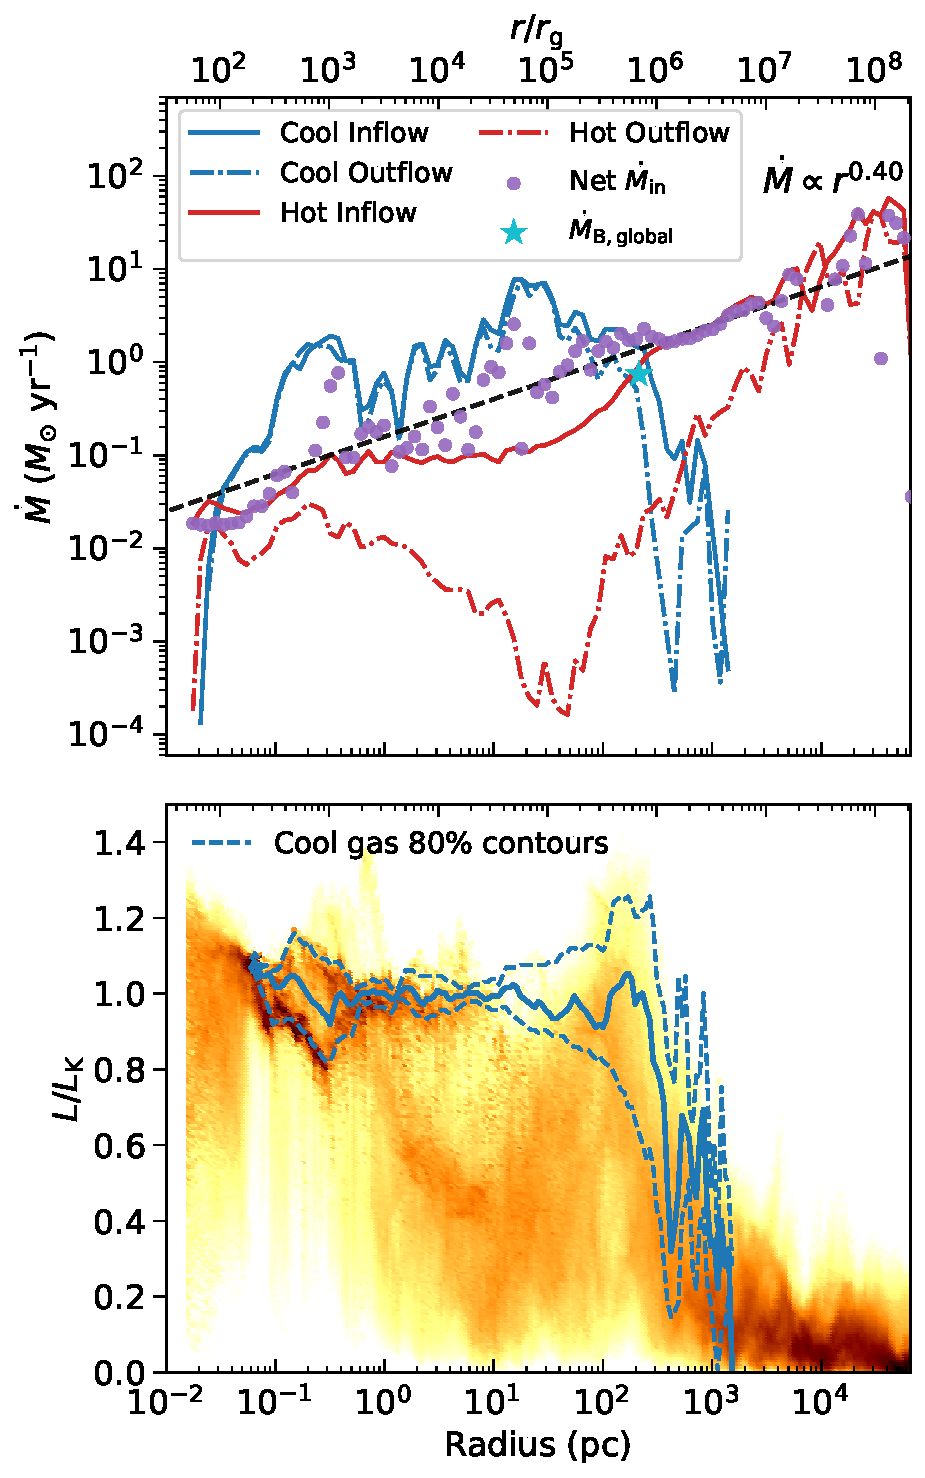
\includegraphics[height=0.65\textheight,keepaspectratio]{Sim_img/angular-momentum_m-dot_930.pdf}
    \caption{Top: Inflow/outflow rates of the multiphase gas. The inflow component is plotted in solid lines, while the outflow component is in dotted-dashed lines. Purple dots are the net inflow, and the black dashed line is a fit for the net inflow, which follows the relation $\dot{M} \propto r^{0.40}$. The teal star shows the global Bondi accretion rate of the system (\mdot$_{\rm B,global}$, see Section~\ref{sec:bondi-discussion}), which is roughly equal to the net inflow rate of hot gas at the same radius. Bottom: Distribution of hot gas total angular momentum, normalized by the Keplerian angular momentum ($L/L_{\rm K}$). Darker shades indicate higher fractions of gas at each radial bin. Blue solid line is the cool gas mass-weighted angular momentum radial profile, bracketed by two dashed lines that represent the 10th and 90th percentiles of the cool-gas distribution.\label{fig:l-m-dot-meso}}
\end{figure}

\begin{figure}
    \centering
    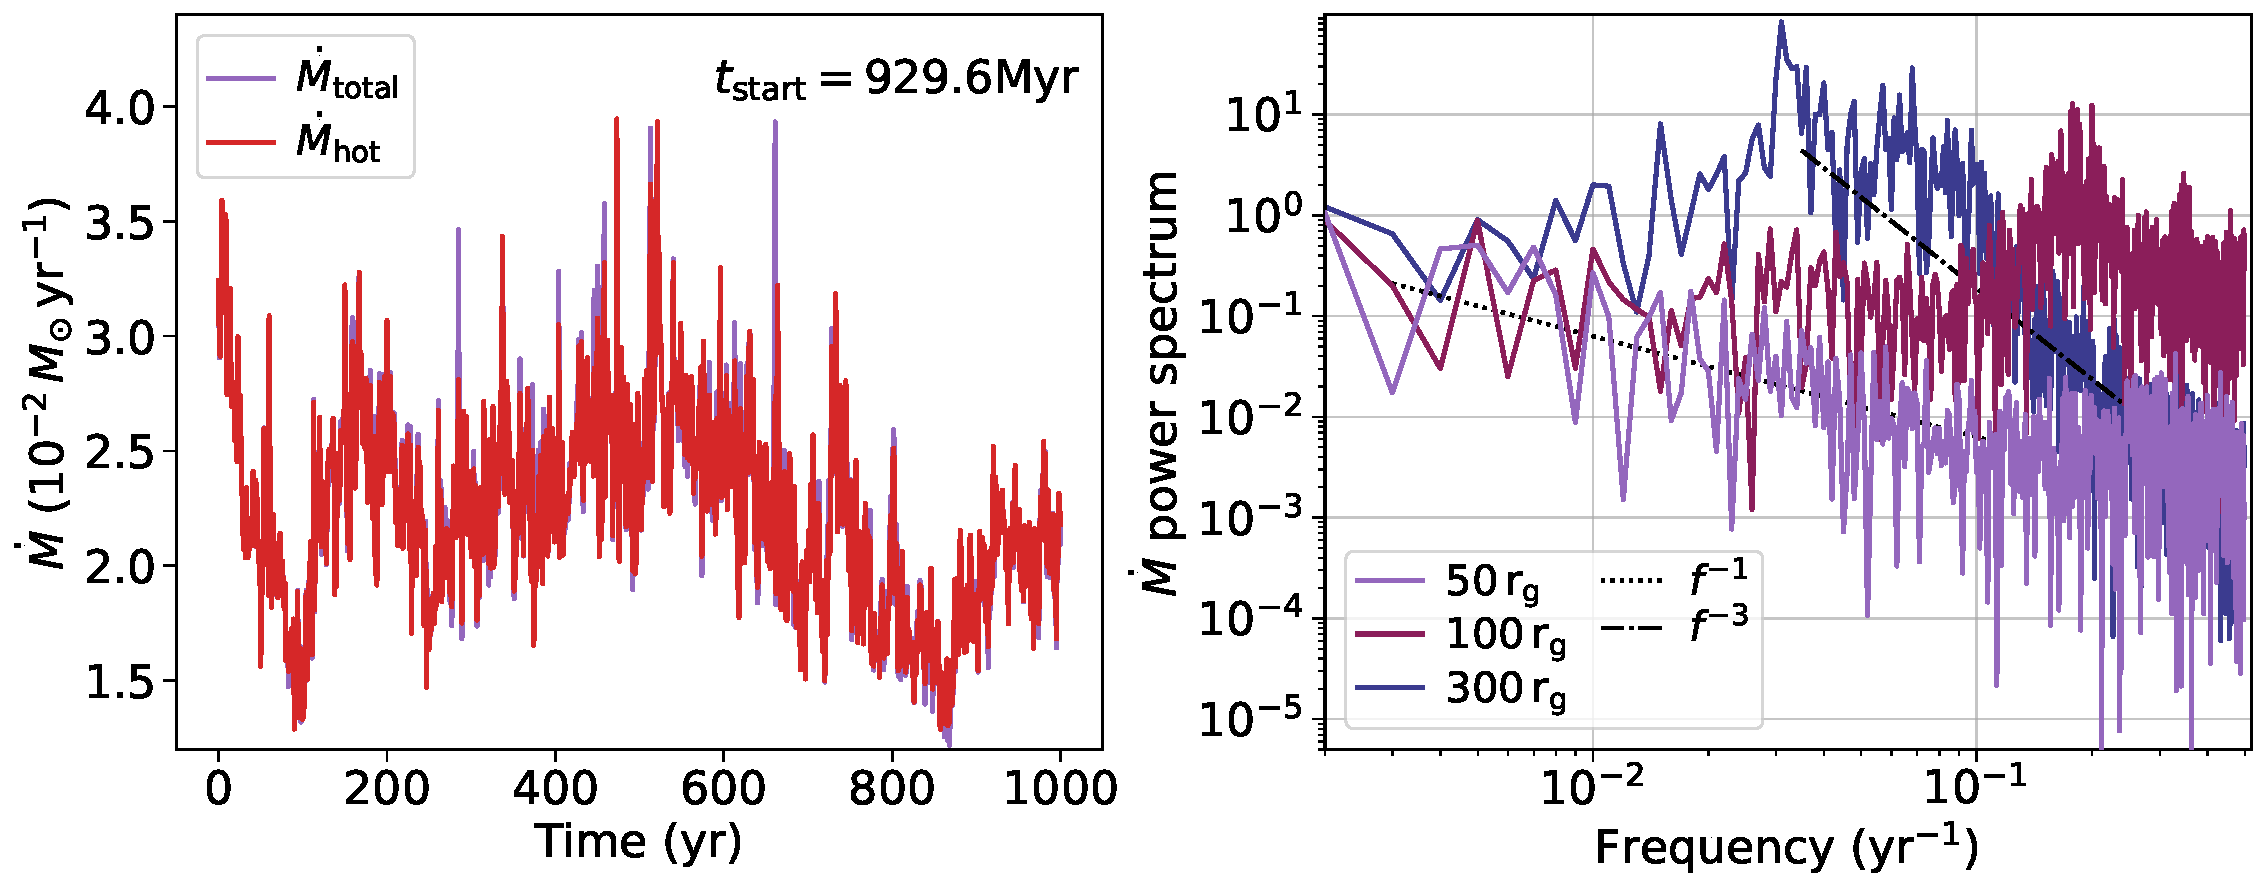
\includegraphics[width=\linewidth]{Sim_img/mdot_meso_930.pdf}
    \caption{Left: \mdot\ measured at the inner boundary, $R_{\rm acc,R20}\approx 16$\,mpc $\approx 50\,r_{\rm g}$, of the hot gas (red) and total gas (purple). Virtually all cool gas has been compression-heated into the hot phase, so the cool gas accretion rate is regularly $\gtrsim 2$\ orders of magnitude below the hot gas accretion rate. We have therefore omitted the line here for clarity. Right: power spectrum of \mdot, measured at $r \approx 50\,r_{\rm g} \approx R_{\rm acc,R20}$ (purple), at $r = 100\,r_{\rm g} \approx 31$\,mpc (magenta), and at $r = 300\,r_{\rm g} \approx 0.1$\,pc (dark blue). The dotted and dotted-dashed lines are reference slopes for the spectra.\label{fig:m-dot-meso}}
\end{figure}

We also examine the motion of the cooling flow through its angular momentum distribution in the lower panel of Figure~\ref{fig:l-m-dot-meso}.
The cool gas does not exist in significant quantities beyond $r \sim 2$\,kpc.
Cool gas initially possesses low angular momentum as it precipitates out of the hot halo ($L_{\rm cool}/L_{\rm K}\approx0.4$), before settling onto rotationally supported disks inside $\sim 200$\,pc.
The cool gas remains in Keplerian disks ($L_{\rm cool}/L_{\rm K}\approx1$) all the way until it disappears at $\sim 6\times10^{-2}$\,pc.

At large scales, $r\gtrsim 1$\,kpc, the hot gas motion is predominantly radial ($L_{\rm hot}/L_{\rm K} \lesssim 0.2$).
Inside $\sim 1$\,kpc, hot gas is found with a wide range of angular momentum, with a roughly uniform spread in the range $0 < L_{\rm hot}/L_{\rm K} \lesssim 1$.
At $1\,\mathrm{pc} \lesssim r \lesssim 200$\,pc, the hot and cool phases are kinematically decoupled.
Inside $r \sim 5\times10^3\,r_{\rm g} \approx 1\,$pc, the two phases begin to overlap in angular-momentum space, as can be seen by the cospatiality between the hot gas angular momentum distribution and the 80th-percentile contours of the cool gas in Figure~\ref{fig:l-m-dot-meso}.
At these scales, gas from the cool disk is heated above the $10^6\,K$ threshold, turning into hot gas, while retaining substantial rotational support.
This heating process concludes at $\sim 6\times10^{-2}\,$pc, where the cool phase is completely depleted.
Inside this scale, the hot gas angular-momentum distribution spreads out more widely, spanning $0 < L_{\rm hot}/L_{\rm K} \lesssim 1.3$.

\subsubsection{Accretion variability} \label{subsec:variability}

We study both the total accretion rate through the smallest accretion zone ($R_{\rm acc,R20}=4^2\,\mathrm{mpc}\approx 50\,r_{\rm g}$) and its associated variability in this subsection. For this analysis, we rerun the meso-scale simulation (R20) at $t\approx930$\,Myr and record the accretion rate with a one-year cadence, over $\Delta t = 1$\,kyr.
Throughout this period, we observe no significant variability in the accretion rate, with at most a factor of $\sim 2$ difference in \mdotbh\ (see the left panel of Figure~\ref{fig:m-dot-meso}).
The low variability agrees with multi-year X-ray observations of M87 \citep[][]{prieto_central_2016,cheng_year-scale_2023}.
Given an average \mdotbh\ over this period of $\approx 2.2\times10^{-2}\, \mathrm{M_{\odot}\,yr^{-1}}$, the inferred jet power, using Equation~\ref{eq:jet_power} with $\eta \approx 10^{-4}$, is $\mathcal{P}_{\rm jet} \approx 10^{41}\,\mathrm{erg\,s^{-1}}$.

We estimate the AGN jet variability by computing the $\dot{M}$\ power spectrum at three distances from the SMBH in the meso-scale simulation: (1) at the inner boundary, $r = R_{\rm acc,\,R20}\approx 50\,r_{\rm g}$, (2) at $r = 100$\,\rg, and (3) at $r = 300$\,\rg\,$\approx 0.1\,$pc, and plot them in the right panel of Figure~\ref{fig:m-dot-meso}.

At the accretion zone, the power spectrum is shallow, approximately $S\propto f^{-1}$, indicating weak variability in \mdot, and thus in the jet power, over the 1\,kyr evolution. The same behavior is also observed in the time series shown in the left panel. At $r=100$\,\rg, the spectrum has a different shape: it steepens to $S\propto f^{-3}$ at high frequencies ($f\gtrsim0.1\,\mathrm{yr^{-1}}$), but flattens at lower frequencies. This suggests that the accretion rate varies on short, year-to-decade timescales, while remaining comparatively stable over longer timescales. The same radius also marks the flattening of the \mdot\ radial profile (see Figure~\ref{fig:l-m-dot-meso}).
At $r = 300$\,\rg\,$\approx0.1$\,pc, the power spectrum remains at a steep $-3$ slope over a larger range of frequencies.
The $f^{-3}$ portion appears to extend to lower frequencies as the measurement radius increases.
Overall, however, it is difficult to ascertain the significance of the results at these scales due to the many potentially important physical processes not accurately captured by our hydrodynamic simulation, such as magnetic and relativistic effects.
We discuss these limitations in further detail in Section~\ref{subsec:limitations}.

\subsection{Discussion} \label{sec:discussion}

\subsubsection{Bondi accretion model in the context of multiphase, inhomogeneous accretion} \label{sec:bondi-discussion}

\begin{figure}
    \centering
    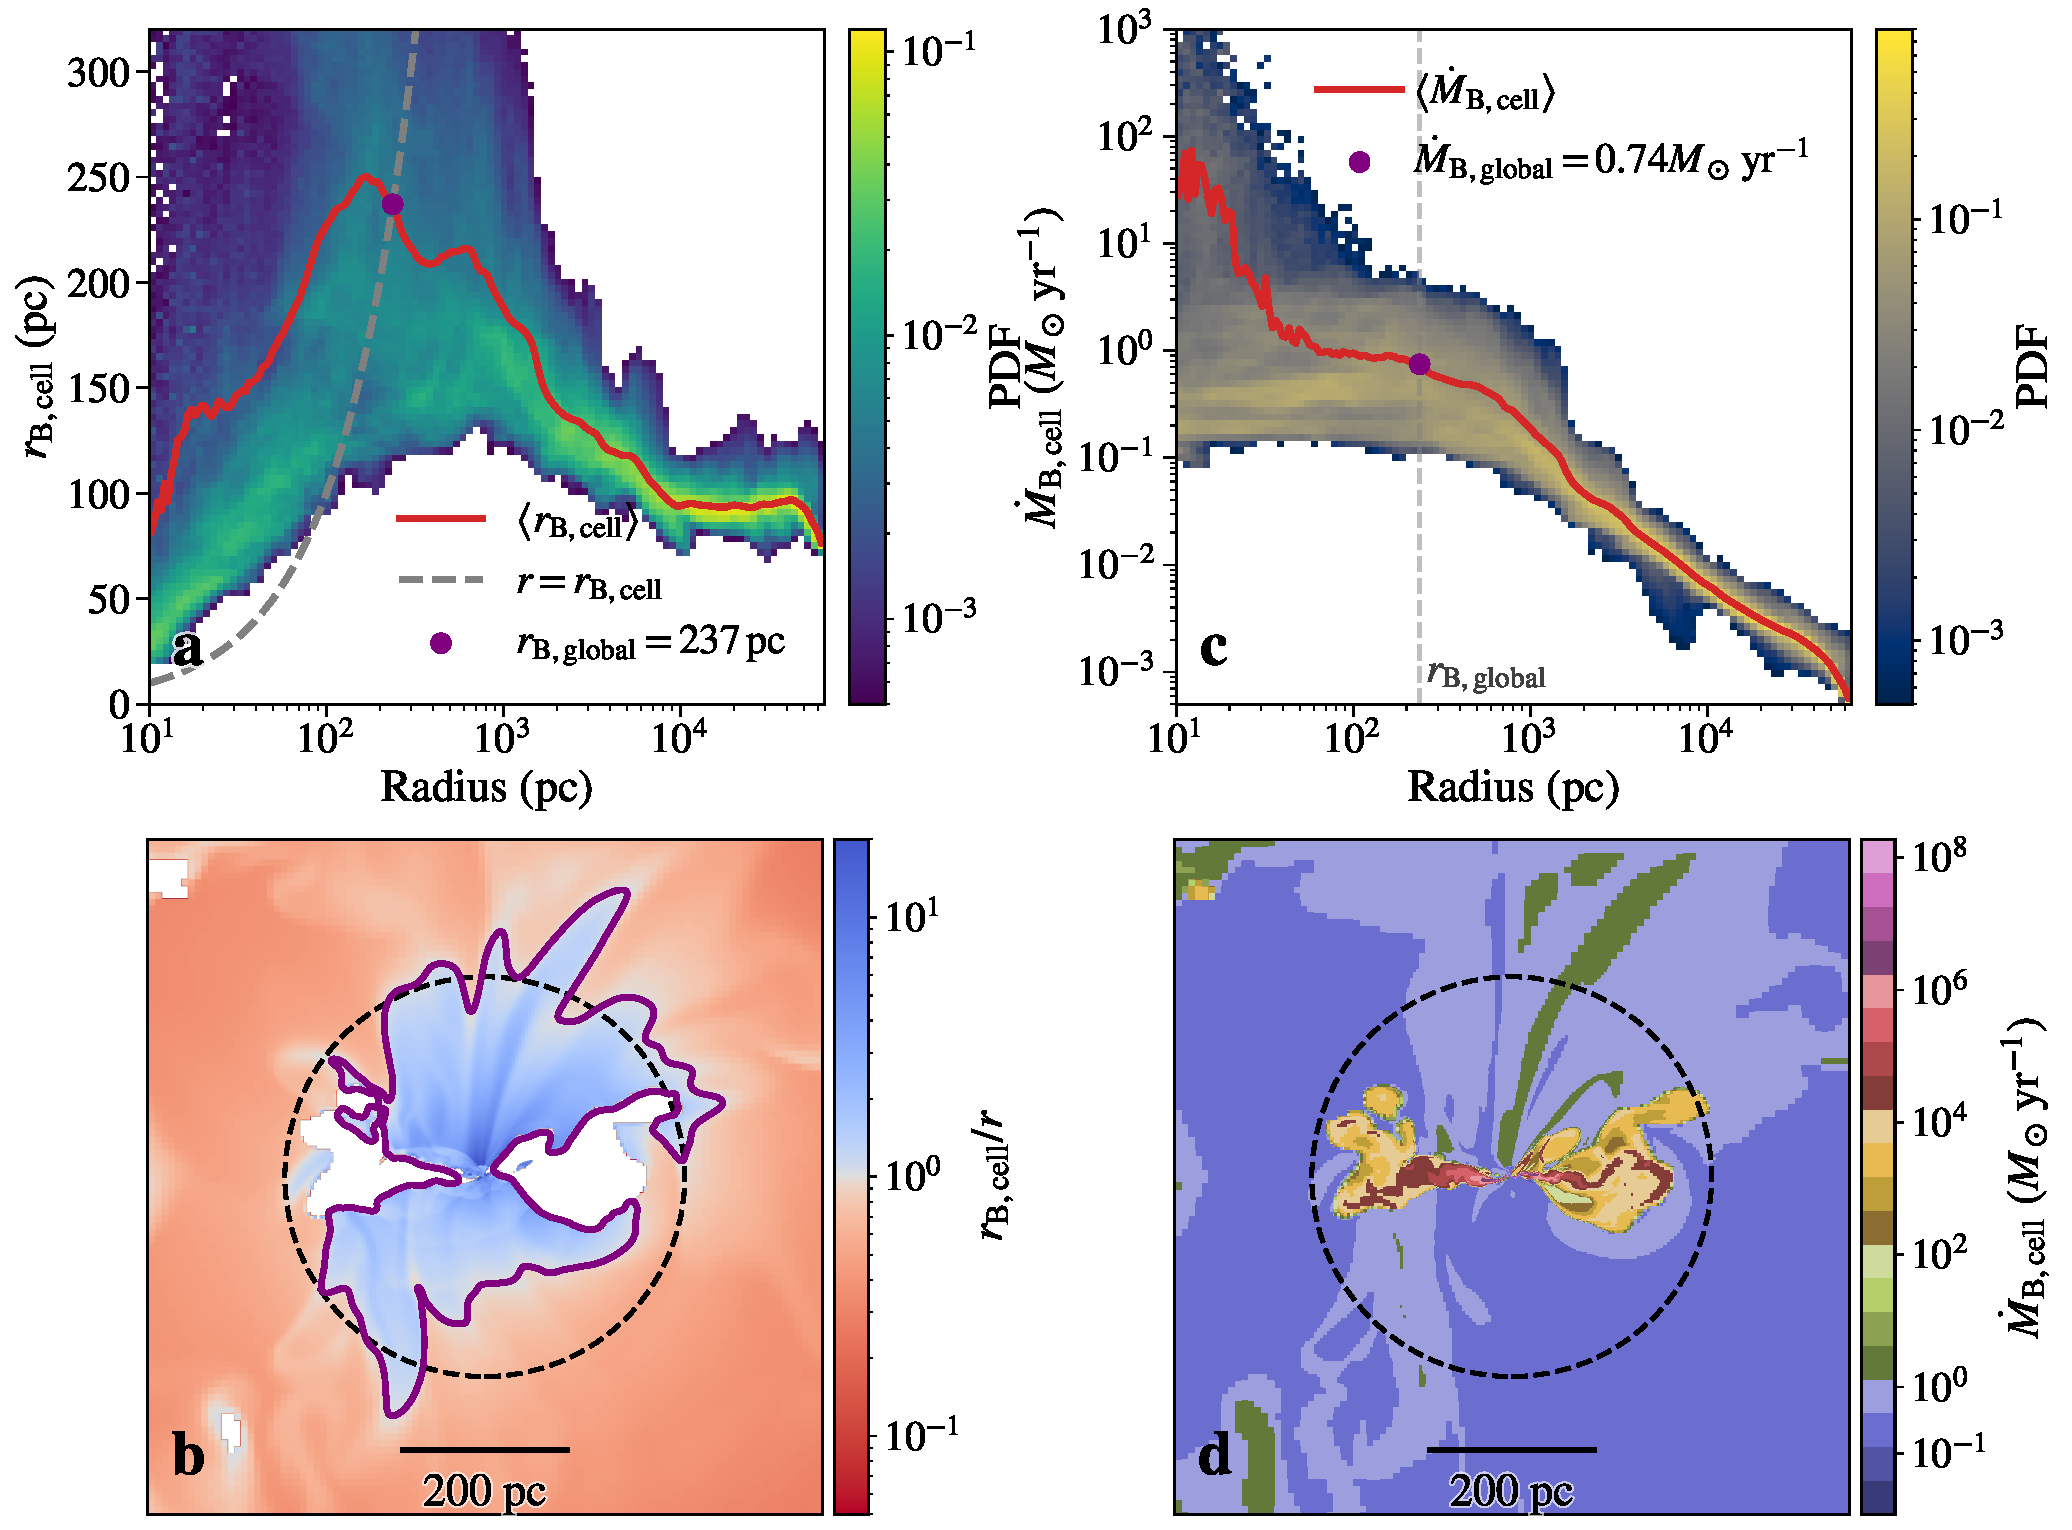
\includegraphics[width=\linewidth]{Sim_img/bondi_analysis_930.pdf}
    \caption{(a) Probability density function, normalized by each radial bin, of the cell-level Bondi radius (following Equation~\ref{eq:rb}) as a function of distance from the black hole. The red line shows the mass-weighted average ($\langle r_{\rm B,cell}\rangle$) radial profile. We approximate a global Bondi radius of the system as the location where $\langle r_{\rm B,cell}\rangle = r = 237$\,pc (purple dot).
    (b) $yz$-slice plot of $r_{\rm B,cell}/r$, with gas below the Bondi-analysis temperature cut ($T < 5 \times 10^6\,\mathrm{K}$) masked out. The purple contour denotes the real Bondi surface of this system (where $r_{\rm B,cell}/r =1$), which is distinctly non-spherical compared to the black dashed circle of radius $r = r_{\rm B,global}$.
    (c) Same as (a), but for the cell-level Bondi accretion rate (following Equation~\ref{eq:m-dot-bondi}). We estimate a global Bondi accretion rate of the system as $\dot{M}_{\rm B,global} \equiv \langle \dot{M}_{\rm B,cell}\rangle (r=r_{\rm B,global}) = 0.74\,\mathrm{M_{\odot}\,yr^{-1}}$.
    (d) $yz$-slice plot of $\dot{M}_{\rm B,cell}$. The Bondi accretion rate in the hot phase is in line with observational expectations, $\dot{M}_{\rm B,\ hot} \sim 0.1\, \mathrm{M_{\odot}\,yr^{-1}}$.\label{fig:bondi-m-dot-r}}
\end{figure}

The classical Bondi accretion model assumes a spherically symmetric accretion flow of a single-phase medium onto a point mass---the SMBH at the center of a galaxy.
Within this accretion flow, there exists a distance from the black hole at which the escape velocity of the gas equals its sound speed.
This distance, the Bondi radius, is expressed as:
\begin{equation}\label{eq:rb}
    r_{\rm B} = \frac{2GM_{\rm BH}}{c^2_{s}},
\end{equation}
where $G$\ is the gravitational constant, $M_{\rm BH}$\ is the black hole mass, and $c_{s}$\ is the sound speed of the single-phase medium.
For the hot gas in M87, \textit{Chandra} measurements give a central temperature of $k_{\rm B}T \approx 0.9$\,keV, implying $r_{\rm B} \approx 120$--$220$\,pc \citep{russell_inside_2015}.

The Bondi accretion rate can be computed as the mass flux through the surface of the Bondi sphere:
\begin{equation}\label{eq:m-dot-bondi}
    \dot{M}_{\rm BH} \approx \dot{M}_{\rm B} = \frac{4\pi G^2 M^2_{\rm BH}\rho}{c^3_{s}}\,.
\end{equation}
In M87, the inferred Bondi accretion rate using the observed X-ray density and temperature is \mdotb\,$\approx 0.1\,\mathrm{M_{\odot}\,yr^{-1}}$\ \citep[][]{russell_inside_2015}.

\centerline{\textbf{The limitations of the traditional Bondi model}} \label{subsec:bondi-limit}

The Bondi model makes several key assumptions about the accretion flow that do not accurately reflect the environment around AGNs.

Firstly, observations have detected multiphase gas inside the Bondi radius in several nearby systems, both in \halpha\ \citep[e.g.,][]{conselice_nature_2001,boselli_virgo_2019} and the molecular phase \citep[e.g.,][]{combes_alma_2019, hsieh_circumnuclear_2021}.


Secondly, the hot phase is inhomogeneous, and hot accretion is rarely spherically symmetric. X-ray measurements of line widths toward cluster cores have suggested that the hot phase is turbulent \citep[e.g.,][]{zhuravleva_turbulent_2014,hitomi_collaboration_atmospheric_2018}. Significant outflows also originate from inside the Bondi radius, from both black hole feedback \citep[e.g.,][]{mcnamara_heating_2005} and stellar feedback \citep[e.g.,][]{hopkins_stellar_2016}.

Thirdly, the inflow rate of gas through the Bondi radius is much larger than the accretion rate onto the SMBH\@. In addition to outflows, cool gas clumps carry some angular momentum as they enter the Bondi sphere and form accretion disks \citep[e.g.,][]{walsh_m87_2013,hsieh_circumnuclear_2021}. The disk provides angular momentum support against infall, which slows down accretion. In M87, accretion rate measurements via the jet mechanical power \citep[][]{broderick_event_2015}, or from Faraday rotation at the nucleus of the galaxy \citep[][]{kuo_measuring_2014} showed that the accretion rate at the event-horizon-scale is two to three orders of magnitude lower than the Bondi accretion rate. The same discrepancy is also seen in multiple GRMHD simulations constructed to inform the EHT result \citep[][]{eht_eight}.


\centerline{\textbf{A new perspective on the ``Bondi sphere''}}

Using our multi-scale simulation, we examine the Bondi accretion model and discuss its applicability in a multiphase accretion flow.
Firstly, we use Equation~\ref{eq:rb} to compute the Bondi radius, $r_{\rm B,cell}$, for gas with $T \geq 5\times10^6\,\mathrm{K}$, equivalent to $k_{\rm B}T \geq 0.43$\,keV, in each grid cell.
We adopt this stricter temperature cut to isolate the gas near the virial temperature; cooler gas has a lower sound speed and therefore much larger values of both \rb\ and \mdotb.
Then, we present a range of $r_{\rm B,cell}$ values across radial distances with a phase plot in Figure~\ref{fig:bondi-m-dot-r}a.
At small radial distances, the spread in the $r_{\rm B,cell}$ values is large, corresponding to large fluctuations in the hot gas temperature.
Outside $r \sim 3$\,kpc, the distribution becomes less variable and settles around $r_{\rm B,cell}\,\approx 100$\,pc.

As one moves along a radial line toward the center, there comes a point in space where the inward gravitational force overtakes the outward force exerted by the thermal gas pressure.
We identify such a point by tracking the ratio between a cell's Bondi radius and its radial distance, $r_{\rm B,cell}/r$. The isosurface tracing $r_{\rm B,cell}/r = 1$\ is the true ``Bondi surface'' of the system.
We visualize this surface as a purple contour in Figure~\ref{fig:bondi-m-dot-r}b. The gas inside this boundary is expected to accrete at supersonic speed.
The Bondi surface replaces the Bondi sphere in a turbulent, inhomogeneous accretion flow.
We find the true Bondi accretion rate by computing the net inflow rate through this surface:
\begin{equation}\label{eq:true-mdotb}
    \dot{M}_{\rm B,surface} = -\oint_S \rho \mathbf{v}\cdot d\mathbf{A},
\end{equation}
where $\rho$\ is the gas density, $\mathbf{v}$\ is the velocity vector, and $d\mathbf{A}$\ is the outward-pointing area element. The inferred net accretion rate using Equation~\ref{eq:true-mdotb} is $\dot{M}_{\rm B,surface} = 1.2\,\mathrm{M_{\odot}\,yr^{-1}}$.


\centerline{\textbf{Estimating Bondi accretion rate with our proposed model}}

In practice, most modern cosmological simulations (as well as X-ray observations) are not able to resolve the complex morphology of the Bondi surface.
Nevertheless, we can still extract useful information about the accretion flow by approximating a Bondi radius of the whole system.
We obtain a mass-weighted radial profile of $r_{\rm B,cell}$ (Figure~\ref{fig:bondi-m-dot-r}a, red line), then define the global Bondi radius to be where $r = \langle r_{\rm B,cell} \rangle$\ (Figure~\ref{fig:bondi-m-dot-r}a, purple dot).
In the R20 simulation at $t\approx930$\,Myr, $r_{\rm B,global}=237$\,pc.
This value is approximately equal to a volume-equivalent radius of the Bondi region, $r_{\rm B,surface} = r[\int dV(r_{\rm B,cell}/r\geq 1)] = 214$\,pc.

We then use Equation~\ref{eq:m-dot-bondi} to compute the Bondi accretion rate of the hot gas cell-by-cell.
In contrast with the $r_{\rm B,cell}$ distribution, the distribution of $\dot{M}_{\rm B,cell}$ as a function of radius shows much less scatter and generally plateaus around $0.1$--$1\,\mathrm{M_{\odot}\,yr^{-1}}$ between $\sim10$\,pc and $10^3$\,pc.
This plateau can be explained by the relatively flat profiles of gas density and temperature over this scale range (see Figure~\ref{fig:r-prof-meso}).
\citet{li_simulating_2012} suggested that this flatness is a result of a self-regulated balance between adiabatic compression and cooling, and depends strongly on the gravitational profile of the stellar (brightest cluster galaxy) potential.
The global Bondi accretion rate, obtained by taking the mass-weighted value of $\dot{M}_{\rm B,cell}$ at $r_{\rm B,global}$, is $\dot{M}_{\rm B,global} = \langle \dot{M}_{\rm B,cell} \rangle \approx 0.74\,\mathrm{M_{\odot}\,yr^{-1}}$.
This value is within one order of magnitude of earlier estimates from \textit{Chandra} X-ray observations \citep{di_matteo_accretion_2003, russell_inside_2015}, and is also consistent with the true Bondi accretion rate of the system, $\dot{M}_{\rm B,surface} = 1.2\,\mathrm{M_{\odot}\,yr^{-1}}$.
However, one important distinction between our system and the Bondi model is that a large amount of cool gas contributes to the overall accretion flows, which dramatically boosts the inflow rate at the \rb\ scale (see Figure~\ref{fig:l-m-dot-meso}).
Even the new Bondi surface that we introduce here does not account for cool gas accretion.

To further emphasize the disconnect between the Bondi model and galaxies with multiphase gas, Figure~\ref{fig:bondi-m-dot-r}d shows a $yz$-slice ($x=0$) of $\dot{M}_{\rm B,cell}$.
The hot gas permeates the polar region and has $\dot{M}_{\rm B,cell}$ values between $\approx 0.05$ and $\approx 0.2 \,\mathrm{M_{\odot}\,yr^{-1}}$, broadly in line with previous spherically symmetric estimates.
On the other hand, the cool gas accumulates in the equatorial plane and in the tilted disk, with Bondi accretion rates five to nine orders of magnitude above those of the hot phase ($\dot{M}_{\rm B,cell}\lesssim 10^8\,\mathrm{M_{\odot}\,yr^{-1}}$).
Even then, the $\dot{M}_{\rm B,cell}$ values could be much higher if a lower temperature floor was used.
M87$^{\star}$ clearly does not accrete at such a rapid rate, primarily thanks to rotational support of the disk against rapid, direct infall.

\centerline{\textbf{Accretion rate scaling relation for future cosmological simulations}}

Despite its inability to correctly describe the multiphase accretion flows, we find that the Bondi accretion rate provides a good estimate of the net hot gas inflow in all three meso-scale simulations.
For example, in Figure~\ref{fig:l-m-dot-meso}, the teal star, which is the approximate Bondi accretion rate of the system, $\dot{M}_{\rm B,\,global}$, sits directly on the solid red line (hot inflow).
Given these observations and the scaling relation found in Equation~\ref{eq:930_scaling}, the true \mdotbh\ value could be more accurately estimated if one applied the \mrrelation\ scaling relation only to the hot gas at scales beyond which cool gas is found, since at large scales the relation accurately traces the scaling of hot gas accretion.
In our system, cool gas formation begins at $\sim 2$\,kpc from the galactic center (Figure~\ref{fig:r-prof-meso}).
Therefore, cosmological simulations can extract the radial velocity and gas density at some distance $R_{\rm hot} > 2$\,kpc, compute the inflow rate using Equation~\ref{eq:accretion-from-flux}, then scale it using Equation~\ref{eq:scaling} to obtain a \mdotbh\ value.
This treatment could provide a much more accurate estimate of \mdotbh\ than current Bondi assumptions.


\subsubsection{Filamentary, chaotic accretion of cool gas at the galaxy-scale}
\label{subsec:filaments}

Many local AGNs exhibit extended multiphase, filamentary structures at the $1$--$10$\,kpc scale, which have been observed in both \halpha\ \citep[][]{conselice_nature_2001,olivares_ubiquitous_2019} and CO \citep[][]{edge_detection_2001,mcnamara_1010_2014}.
The origin of these cold filaments could be linked to interactions between SMBH feedback and the gas inside the host galaxy \citep[][]{cavagnolo_entropy_2008,tremblay_cold_2016}.
At the sub-kpc scale, multiphase disky structures have also been observed in these systems.
In M87, a circumnuclear disk is observed inside the Bondi radius \citep[][]{walsh_m87_2013,osorno_revisiting_2023}.
In the Perseus cluster, recent observations have detected an even larger disk-shaped structure extending out to $r\sim 10$\,kpc \citep[][]{vigneron_high-spectral-resolution_2024}.
Cold clumps can circularize around the SMBH thanks to conservation of angular momentum, creating these disky structures.

Large-scale filamentary structures have also been seen in multiple numerical studies of galaxy clusters \citep[e.g.,][]{li_2014b,eisenreich_active_2017,beckmann_dense_2019}.
In simulations with longer evolutions ($\Delta t\gtrsim1\,$Gyr), a kpc-scale disk is often seen \citep[e.g.,][]{li_2014a,prasad_cool_2015,wang_agn_2019}.
This disk can be dynamic as it is disrupted by the AGN jet or destroyed through accretion \citep[][]{prasad_cool_2015}, then reforms from further cooling.
At different times, the disk can have completely different dynamics, most notably in its random rotation axis.
We observe the same large-scale disk morphology in our fiducial simulation.
Figure~\ref{fig:thermodynamics} shows a few examples of these ever-changing disk dynamics.
Earlier in the galaxy evolution, cool gas accretion onto the inner boundary is facilitated by direct infall of cool filaments.
Starting around $t \sim 0.8$\,Gyr, cool filaments with higher angular momentum start to accumulate around the accretion zone, creating disky structures.
For the following few hundred Myr, we observe periods when the filamentary phase and the disky phase alternately dominate.
Lastly, a large-scale ($R_{\rm disk} \sim 0.5$--$1$\,kpc), sustained disk is found around the accretion zone for the remainder of the simulation.
Interestingly, however, the disk's rotation axis changes significantly with time, even after the large-scale disk has formed.
The disk's angular momentum vector is controlled by how and where the cool gas clumps originate.



Most earlier numerical studies found disky tori which extend beyond several kpc in scale after $\sim 1$\,Gyr.
One key difference between these results is that while the disk in \citet{li_2014a,li_2014b} is stable for several Gyr, the disk in \citet{prasad_cool_2015} and in \citet{wang_agn_2019} dissipates over time, before repeating the formation cycle.
Our results show the large-scale disk can dissipate before $\sim 1.2$\,Gyr, but then stabilizes from this point onward.
We propose that how early the disk forms and its stability depend strongly on the size of the accretion zone.



To better understand this dependence, we carry out an experiment.
At time $t=920\,$Myr, the cool gas filaments accrete with large radial velocities and appear quite chaotic down to the inner boundary (Figure~\ref{fig:resolution-exhibit}a), similar to structures seen in previous multiphase accretion simulations \citep{beckmann_dense_2019,guo_magnetized_2024}.
We then evolve this snapshot in the following two ways:

First, we obtain higher cadence output of the fiducial simulation with 8 levels of SMR for the next 100\,Myr.
The filamentary and radial accretion of cool gas continues for several Myr (Figure~\ref{fig:resolution-exhibit}b).
These filaments actually possess a small amount of angular momentum, but this is not enough to circularize the gas around this large accretion zone ($R_{\rm acc,R8} \approx 65$\,pc), and the angular momentum is then removed together with the accreted gas.
Occasionally, a cool clump with angular momentum ($\ell$) large enough to circularize outside of the accretion zone appears, and a disk forms.
Once formed, the disk requires a constant supply of angular momentum to replenish its loss through accretion.
Such conditions are less common when the inner boundary of the simulation is sufficiently large, and thus we see that filamentary, chaotic accretion dominates the early evolution of the fiducial simulation ($t \lesssim 1$\,Gyr).

Second, we add two additional levels of nested SMR to the center and shrink the accretion zone by a factor of four compared to the fiducial simulation ($R_{\rm acc,R10} \approx 16$\,pc).
Now, it takes much less initial angular momentum for a cool clump to circularize around the accretion zone without being directly accreted (Figure~\ref{fig:resolution-exhibit}c).
A disk formed at smaller scales also requires less angular momentum to balance the amount lost through accretion, and is therefore more stable and can grow over time.

We also quantify the disk's stability by looking at the 100-Myr time evolution of the angular momentum in the fiducial and refined cases, which is plotted in the bottom two panels of Figure~\ref{fig:resolution-exhibit}.
In the first 10\,Myr, the two time series share similar characteristics and appear quite chaotic.
During the final 90\,Myr, the refined R10 run forms and retains a Keplerian disk at $r = R_{\rm acc,R8} \approx 65$\,pc, whereas the fiducial R8 run repeatedly forms and disrupts a disk as its angular-momentum direction changes.
This resolution dependence suggests that an oversized accretion zone can remove gas before a $\sim 10$--$100$\,pc disk circularizes.
The persistent disk in R10 resembles those in \citet{li_2014a,li_2014b}, whereas the episodic behavior in R8 resembles that reported by \citet{prasad_cool_2015}.
We therefore infer that some earlier simulations may contain unresolved circumnuclear disks concurrent with kpc-scale filaments.
This inference is also consistent with observations, as molecular disks have been observed with ALMA in multiple local AGNs \citep[e.g.,][]{combes_alma_2019,garcia-burillo_galaxy_2021}.



\begin{figure}
    \centering
    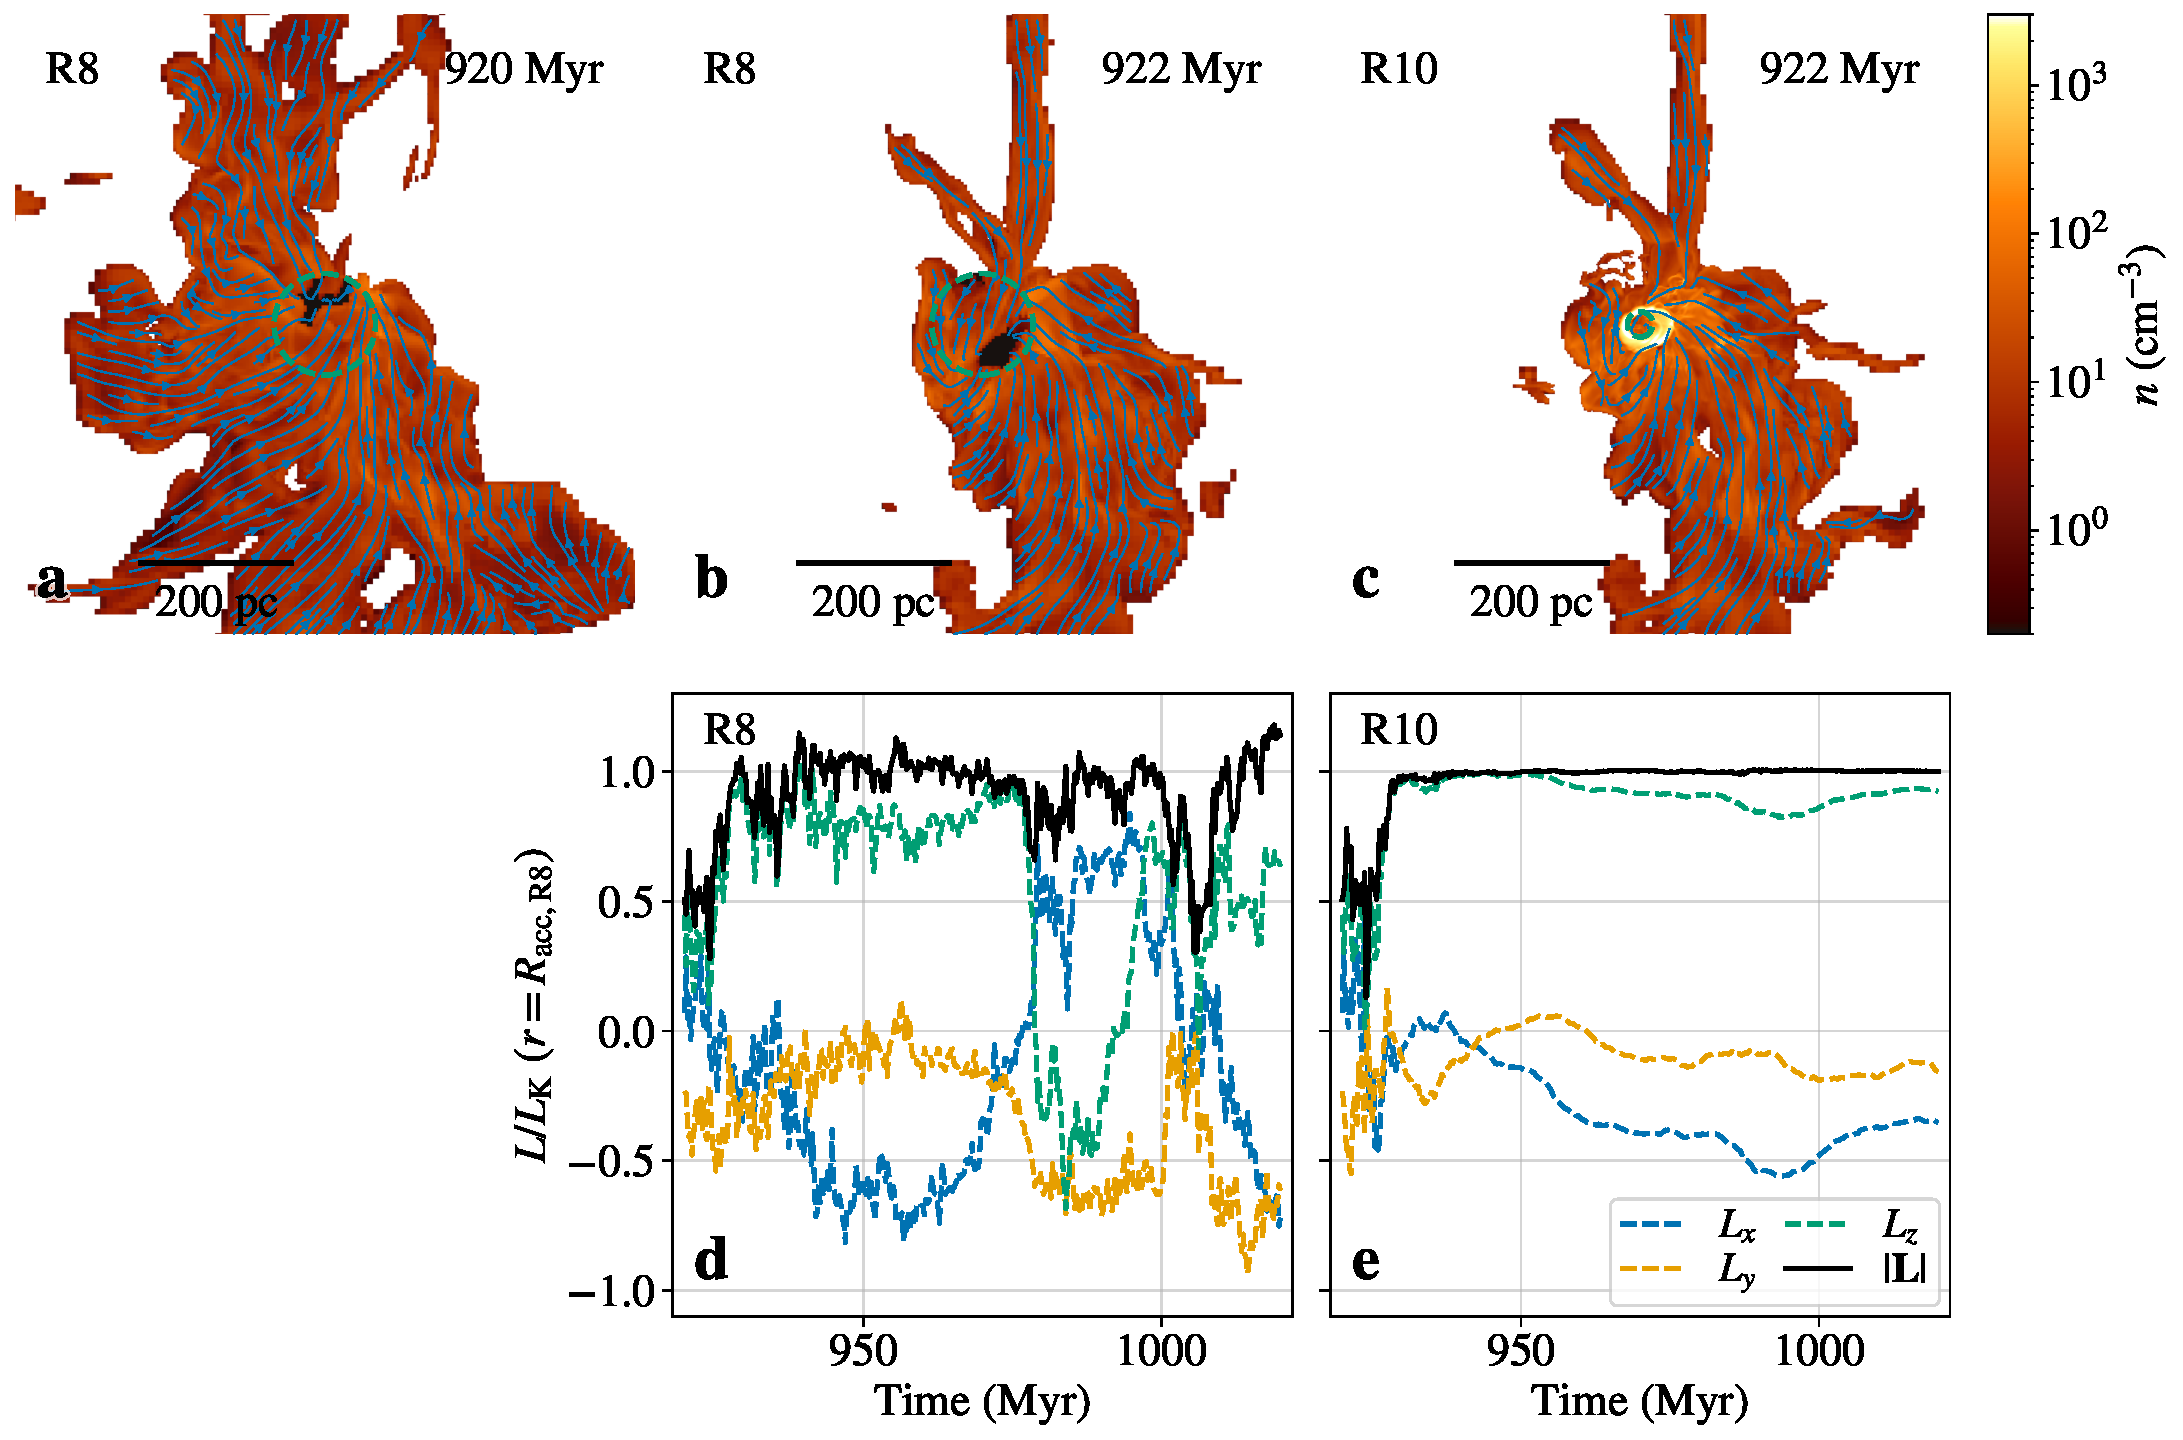
\includegraphics[width=\linewidth]{Sim_img/resolution_exhibit.pdf}
    \caption{
    Top: Projections along the $z$-axis of the number density for the cool gas ($T < 10^6\,K$), with streamlines showing the projected velocity field. Panel (a) shows the fiducial R8 simulation at $t=920\,{\rm Myr}$. Panels (b) and (c) show the evolved morphology at $t=922\,{\rm Myr}$ for the R8 and R10 simulations, respectively. The green dashed circles mark their respective accretion zones. Bottom: normalized specific angular momentum, measured at the same physical radius, $r=R_{\rm acc,R8}\approx65\,{\rm pc}$, for the R8 and R10 runs, recorded over a 100\,Myr evolution. The colored dashed curves show $L_x$, $L_y$, and $L_z$, while the black solid curve shows $|\mathbf{L}|$.
    \label{fig:resolution-exhibit}}
\end{figure}

\subsubsection{Limitations and future work}
\label{subsec:limitations}

The simulations we presented in this work probe gas dynamics across eight orders of magnitude in spatial scale
and nine orders of magnitude in time.
To achieve this vast scale separation, we omit several physical processes which we do not expect to have a significant impact on the overall gas distribution.
Here, we discuss the potential effects of these neglected processes.

Our simulations are purely hydrodynamic and neglect the effects of magnetic fields.
In galaxy clusters, the ICM is weakly magnetized, with plasma $\beta \sim 10^2$--$10^3$ (the ratio between thermal pressure and magnetic pressure).
In the hot phase, \citet{guo_magnetized_2024} found that magnetic energy becomes dynamically important around $r \sim 10^4$\,\rg.
In the cool phase, $\beta \sim 1$\ even at scales $\gtrsim 10^5$\,\rg. Magnetic fields appear to enhance angular momentum loss in the cool phase, which could shrink the disk by a factor of $\sim 10$\ \citep[e.g.,][]{wang_chaotic_2020}.
In the meso-scale simulation, our cool disk extends to $R_{\rm disk}\approx600$\,pc; a $10\times$\ smaller disk would appear consistent with \textit{HST} observations of a circumnuclear disk at the 40\,pc scale \citep[][]{walsh_m87_2013}.
We expect the qualitative results of a galaxy-scale MHD simulation to be similar to the hydrodynamic case, but the radial extent of the cool gas might differ.
At the meso-scale, magnetic flux advected by the large-scale accretion flow dictates the field geometry of the accretion disk \citep[][]{lubow_magnetic_1994}.
Jet production also depends on the magnetic pressure within the accretion flow \citep[e.g.,][]{proga_magnetohydrodynamic_2005}.

Our simulations employ a relatively high temperature floor, $T_{\rm floor} = 2\times 10^5$\,K.
We use this temperature floor for two reasons: (1) a lower temperature floor results in more restrictive time steps, and (2) the current resolution is insufficient to resolve the scale height of the cool disk at lower temperatures.
We run the R14 simulation at $t\approx1460$\,Myr with $T_{\rm floor} = 10^4$\,K for $\Delta t= 2\,$Myr, and find that the overall gas distribution remains consistent with the fiducial runs, but the disk quickly loses thermal pressure support and collapses vertically such that the large-scale disk becomes a thin disk ($H/R < 0.1$).
Similar behavior was seen in earlier studies \citep[e.g.,][]{guo_toward_2023}.

We do not track star formation in our simulations. The star formation rate in M87 is several orders of magnitude lower than the black hole accretion rate, $\sim 10^{-5}$--$10^{-3}\,\mathrm{M_{\odot}\,yr^{-1}}$ \citep[e.g.,][]{tan_star-forming_2005,tamhane_constraining_2025}, thanks to efficient star-formation quenching by AGN feedback.
Supernova (SN) feedback and stellar winds from AGB stars are also neglected.
These processes would inject energy into the ISM, but would not meaningfully alter the ICM gas dynamics, since jet feedback is the dominant mode of heating at large scales.
At the pc and sub-pc scales, however, Type Ia SNe have been shown to provide significant local heating in the ISM \citep[][]{li_impact_2020}.
Future work will explore how SN feedback in the circumnuclear disk affects the galaxy's turbulent dynamics.

As discussed in \fullsectionref{subsec:meso}, jet feedback is turned off in the R16, R18, and R20 meso-scale simulations.
With magnetic fields, the jet would emerge self-consistently at the meso-scale, ensuring that heating is continuous as we zoom in to the center, as demonstrated by \citet{guo_magnetized_2024}.


\subsection{Conclusions} \label{sec:conclusion}

We introduce a suite of simulations of a radio-mode elliptical galaxy, using initial conditions informed by \textit{Chandra} observations of M87 and the Virgo cluster.
We model the multi-scale, multiphase accretion onto M87 by implementing a hyper-refinement scheme, progressively adding more nested refinement levels to the center of lower-resolution simulations.
This scheme allows us to study the multiphase gas formation at the $\sim$\,kpc scale facilitated by AGN-jet-driven turbulence, then follow the accretion flow down through the meso-scale to just beyond the event-horizon-scale ($r\sim 100$\,\rg).

In this paper, we introduce our simulations, present a study of the overall multiphase dynamics, and examine the inflow-outflow solution at different length- and time-scales.
Our simulations recover the filamentary cool gas formation at the $\sim$\,kpc scale, induced by interactions between the jet and the galaxy (see Figures~\ref{fig:thermodynamics} and~\ref{fig:resolution-exhibit}).

The cool gas filaments carry angular momentum and circularize into a disk around the inner boundary of the simulation (Figures~\ref{fig:zoom-in-proj} and~\ref{fig:l-m-dot-meso}).
Outside $10^3$\,\rg, the motions of the hot and cool phases are completely decoupled. The cool gas exists primarily in Keplerian disks; the hot gas moves more radially. Inside $10^3$\,\rg, the cool gas is compression-heated to higher temperatures and results in a hot accretion disk at the smallest scale probed by our meso-scale simulation (top panel of Figure~\ref{fig:l-m-dot-meso}).

At the galaxy-scale, cool gas accretion dominates over hot gas accretion, often by a factor of $10$\ or more.
This behavior holds true throughout the length scales, down to $\sim 200$\,\rg\ where the cool gas is heated to much higher temperatures, leaving only the hot phase to be accreted through the smallest accretion zone ($R_{\rm acc,R20} \approx 50$\,\rg). The accretion rate is weakly variable in M87 at this scale. The accretion rate at the inner boundary only fluctuates by a factor of $\sim 2$\ over 1\,kyr. In the three high-resolution runs we perform, the profiles of the net inflow rate all follow power-law scalings, $\dot{M} \propto r^k$, where $0.40 \leq k \leq 0.69$. These results broadly agree with previous RIAF simulations that motivate our adopted accretion-rate calibration.

The Bondi model predicts the hot gas net inflow rate, but not the cool gas flow or the \mrrelation\ scaling. We propose estimating \mdotbh\ from the hot gas beyond the cool-gas precipitation radius ($r\gtrsim 2$\,kpc).

Our galaxy-scale simulation shows periods of chaotic, filamentary cool gas accretion, followed by brief disky phases in the first half of its 2\,Gyr evolution. The large-scale disk ($R_{\rm disk}\sim 0.5$--$1$\,kpc) takes over the late-stage evolution. Further examination, however, points toward a constant presence of the disky phase regardless of whether kpc-scale cool filaments are present. We suggest that previous simulations either did not have enough resolution to resolve the circumnuclear disk ($R_{\rm disk}\sim 10$--$100$\,pc), or the accretion boundary was too large to allow cool gas to circularize and form a disk.

\chapter{\texorpdfstring{\MakeUppercase{Summary and Future Outlook}}{Summary and Future Outlook}} \label{chap:summary}

\section{Summary}

This dissertation has followed one common thread across six years of research: modeling astrophysical turbulence across scales by connecting observable tracers, numerical simulations, and machine-learning diagnostics.
Astrophysical turbulence regulates the transport of matter and energy, from galaxy-scale driving down to dissipation scales only a few kilometers across.
Between these extremes in spatial scale lie galactic accretion flows onto active galactic nuclei (AGNs), star formation in molecular clouds, and extreme electromagnetic events near accreting supermassive black holes (SMBHs).
Across these environments, a common difficulty in understanding turbulence is that it is rarely observed directly or numerically modeled without some form of compromise.
Instead, turbulence is often inferred from imperfect tracers and simulations that resolve only part of the dynamical range.
The chapters in this dissertation address these difficulties by developing diagnostic tools tailored to three representative turbulence regimes.

\subsection{Using young stars to study interstellar turbulence}

In Chapter~\ref{chap:stars}, I presented a new method to measure the level of turbulence in star-forming regions with young stars.
Historically, turbulence in Milky Way molecular clouds had been measured through line-width observations of gas tracers, including \halpha, \ion{H}{1}, CO, and HCN\@.
These measurements were precise in the plane-of-the-sky position (only limited by the telescope's beam resolution) and line-of-sight (LOS) velocity (inferred from the shift in wavelength of the tracer), but they provided no information about the other three kinematic dimensions.
Gas-based turbulence measurements were, therefore, severely restricted by projection effects, and conclusions drawn through this method had to contend with a multitude of uncertainties.
Using young stars as turbulence tracers significantly reduces these uncertainties.

In \citet{ha_measuring_2021}, we hypothesized that, since young stars are born out of turbulent molecular clouds, the stars would inherit these turbulent statistics at the region scale.
We obtained six-dimensional (6D) kinematics from the Gaia and APOGEE-2 surveys of 1439 stars in the Orion Molecular Cloud Complex and computed the first-order velocity structure function (VSF) for each subgroup in the region.
We found that in regions where star formation is sparse, the VSFs resemble a Kolmogorov turbulent scaling.
This finding supported our hypothesis and indicated that young stars could indeed serve as a tracer of turbulence in certain conditions.
We also found, on the other hand, that the VSFs from dense star clusters (the Orion Nebula Cluster) were less useful, exhibiting no such power-law scaling.
We explained this lack of turbulent scaling as a direct consequence of dynamical relaxation---the motion of newly formed stars is quickly perturbed by nearby stars, changing their trajectories and erasing the memory of turbulence shortly after formation.
We also commented on another limitation of using stars as a turbulent tracer, namely that stars naturally lose their memory of turbulence through drifting over the crossing time of the region.
These limitations restrict the types of regions in which our proposed method can meaningfully provide turbulence constraints in addition to gas tracers.

In \citet{ha_turbulence_2022}, we formalized our proposed method by extending our coverage to four star-forming regions: Orion, Ophiuchus, Perseus, and Taurus.
We also obtained \halpha\ and CO data for direct comparison between stellar and gas tracers.
In agreement with the previous work, we found a universal scaling of turbulence in all four regions, indicating that young stars are effective tracers of turbulence in star-forming regions and that the turbulent cascade is likely controlled by a Galactic-scale driver.
We also identified a characteristic ``bump'' in the VSF of two regions, Orion and Ophiuchus, which we mapped to analytically confirmed supernovae (SNe) that took place several million years ago.
These SNe injected a large amount of kinetic energy into the two systems, raising the level of turbulence, which steepened the slope of the VSFs.
These events also carried over to the \halpha\ VSFs, where the amplitudes of the VSFs in Orion and Ophiuchus were significantly higher than the VSF of stars.
On the other hand, the VSFs of \halpha\ and stars are roughly consistent in the other two regions.
We concluded that SNe inject energy unevenly into different phases of gas, efficiently driving low-density, volume-filling ionized gas such as \halpha, while affecting the high-density, clumpy molecular gas that forms stars differently.
These two papers suggested a complex picture of the Milky Way interstellar medium (ISM), where turbulence can be driven at different scales and inject energy unevenly into different phases.

Since these works were published, the method has been adopted and extended in several studies of nearby star-forming regions and the molecular ISM\@.
\citet{krolikowski_gaia_2021} studied the Taurus-Auriga region with Gaia EDR3, and showed that the stellar velocity structure retains an initial turbulent spectrum similar to Larson's law before being modified by the dynamical evolution of the association.
\citet{zhou_kinematics_2022} applied the same idea to 150 young stellar object (YSO) associations, using their motions to probe molecular cloud turbulence, velocity dispersion--size scaling, isotropy, and the Galactocentric dependence of turbulent energy dissipation.
Then, \citet{zhou_gas_2024} used the same YSO associations as cloud tracers to compare young-star distributions against CO and dust, and connect feedback-driven gas removal to the velocity dispersion--size relation.
More recently, \citet{zhou_kinematics_2025} combined Gaia DR3 YSO proper motions with CO radial velocities to construct a 3D velocity catalog for 102 YSO/molecular cloud complexes, extending our proposed method from local turbulence measurements to Galactic-scale cloud dynamics.
In a related follow-up work, \citet{velguth_probing_2025} returned to the original 6D stellar VSF approach with Gaia DR3 and APOGEE DR17 and examined the resulting velocity statistics' ability to probe the effects of turbulence, SNe, gravity, and magnetic fields on the regions.
These follow-up studies demonstrate that the young-star tracer method is now being used not only to measure turbulence in individual star-forming regions, but also to connect stellar birth kinematics to cloud evolution, feedback, and the large-scale motion of the Galactic ISM.


\subsection{Machine-learning diagnostics of plasma intermittency}

In Chapter~\ref{chap:ml}, I introduced a machine-learning tool that automates the identification of coherent structures in magnetized plasma turbulence, and demonstrated several use cases in an accompanying astrophysics work.
Prior to this work, reconnecting current sheets were identified either manually or through supervised machine-learning classifiers trained on human-labeled examples \citep[e.g.,][]{hu_identifying_2020}. 
While the latter approaches automate the detection step, they inherit the same foundational problem: the definition of a current sheet was never made rigorous. 
Each researcher applied an arbitrary current-density threshold to select candidate regions, then relied on physical intuition to determine whether a polarity reversal qualified as a reconnecting sheet. 
What was missing was not merely automation, but a theory-agnostic, unsupervised framework that could formally define current-sheet structures from the data itself, without importing a pre-existing subjective definition.
In a modern numerical simulation, there are hundreds of potential sites for reconnection at each timestep, making analysis at scale either exceedingly time-consuming or outright impossible.
The machine-learning package developed in this dissertation reduces this workflow to several minutes per snapshot.

In \citet{ha_awesom_2025}, we detailed the development and usage of \awesom, a self-organizing map (SOM) and statistically combined ensemble (SCE) package that provides scalable, theory-agnostic segmentation of large multi-dimensional datasets.
At its core, \awesom\ is based on two Python implementations: \texttt{POPSOM} \citep{yuan_implementation_2018,hamel_vsom_2019}, which carries out single-threaded, stochastic training of SOMs on small datasets, and \texttt{SCE} \citep{bussov_maarja_segmentation_2021}, which stacks the result of multiple independent clustering realizations into a statistically significant set of clusters.
I completely rewrote both packages to improve training and inference time through a series of optimizations and parallelization.
These optimizations allowed the algorithm to process datasets containing over one million points and tens of dimensions for the first time.
I also performed scaling tests to quantify the speedup compared to legacy codebases and reported up to a $100\times$\ acceleration in training time and a $1000\times$\ reduction in memory usage.

Then, in \citet{ha_machine_2025}, we showed how \awesom\ can be used to segment current sheets in turbulent plasma simulations.
We demonstrated its capability in a suite of three simulations: an idealized Harris current sheet, a decaying turbulence box, and a continuously driven turbulence box.
Through feature engineering, we developed a convolutional kernel to specifically highlight the local magnetic polarity reversal of a reconnecting current sheet.
Our analysis using \awesom\ identified not one, but two types of current sheets, which we characterized as ``single current sheets'' and ``double current sheets''.
Single sheets are the well-known structures with a magnetic polarity reversal across their surface, which allows reconnection.
Meanwhile, double sheets form transiently through collisions of Alfv\'en wave packets and may dissipate energy differently than single sheets.
This distinction, and hence its formal characterization via \awesom, is important for modeling plasma heating and non-thermal particle acceleration, especially in subgrid treatments of kinetic-scale dissipation in general relativistic magnetohydrodynamic (GRMHD) black hole accretion simulations.

Recently, \citet{davis_statistics_2025} used \awesom\ to identify current and vorticity sheets in 3D particle-in-cell (PIC) simulations of relativistic pair-plasma turbulence.
They also discussed the possible connection between vorticity sheets and the double current sheets identified in \citet{ha_machine_2025}.
Beyond plasma turbulence, \awesom\ can also support unsupervised classification and discovery in multi-dimensional datasets. \fullsectionref{sec:awesom-beyond-plasma} illustrates this broader use by applying \awesom\ to \halpha\ LOS velocity maps for identifying star-forming regions in the Milky Way.

\subsection{Multi-scale simulations of SMBH feeding and feedback}

In Chapter~\ref{chap:sim}, I presented a suite of hydrodynamic simulations of a giant elliptical galaxy, motivated by X-ray observations of the galaxy M87\@.
M87 is the ideal candidate for numerical modeling, being a local AGN with well-known jet feedback features and a multitude of observations from the cluster scale down to the event-horizon scale.
In the last decade, observations of galaxies and of the accretion flows onto their central SMBHs have reached an unprecedented level of detail \citep[e.g.,][]{walsh_m87_2013,prieto_central_2016,boselli_virgo_2019,eht_one}.
Accretion onto a SMBH dictates its growth as well as its influence on the host galaxy through feedback \citep[][]{kormendy_coevolution_2013}, yet our theoretical understanding of the connection between accretion flows at the galaxy scale and at the event-horizon scale remains largely incomplete.
Powered by the first direct observations of SMBHs by the Event Horizon Telescope (EHT) \citep{eht_one, eht_sgt_one}, the study of multi-scale accretion theory with numerical simulations has recently been revitalized \citep{ressler_ab_2020,guo_toward_2023,hopkins_forged_2024,cho_multizone_2024}.
The study that I presented in this chapter is part of this larger effort.

In \citet{ha_galaxy-_2026}, we discussed the details of these simulations and several aspects of the multiphase accretion flow.
These simulations, run with the code \texttt{Athena++}, include a nested static mesh refinement (SMR) scheme that follows the multiphase gas from 60\,kpc down to $\sim 20\,$mpc, just outside the SMBH\@.
To achieve this vast range of spatial scales, we ran a galaxy-scale simulation with eight levels of SMR, then identified dynamically interesting snapshots for resimulation at higher resolutions.
We also included a jet feedback prescription that aims to balance radiative cooling on large scales.
We found that the cool gas forms by precipitating out of the hot gas in radially aligned filaments, before circularizing into a disk on scales of tens of parsecs.
The net inflow rate of the multiphase gas follows a radial scaling, $\dot{M}\propto r^k$, where $0.40 \leq k \leq 0.69$, in broad agreement with previous results from radiatively inefficient accretion flow studies.
We also discussed Bondi accretion in the landscape of multiphase, turbulent accretion, and concluded that the Bondi model could still be used to estimate the black hole accretion rate, but only for the hot phase of accretion.
These results can help inform more accurate subgrid treatments of black hole feeding and mechanical feedback in future cosmological simulations.

\section{Future Outlook}

\subsection{Toward a Galactic census of stellar turbulence}

Chapter~\ref{chap:stars} showed that young stars can be used as 6D tracers of turbulent motions in nearby molecular clouds.
A natural follow-up to these studies is to move from a small number of well-investigated star-forming regions to a much larger census across the Milky Way.
The APOGEE and BOSS Young Star Survey (ABYSS) in SDSS-V is designed to obtain spectra for more than $10^5$ young stars, including radial velocities that can be combined with Gaia astrometry to reconstruct full stellar phase-space information \citep{kounkel_abyss_2023}.
With public SDSS-V releases now beginning to provide Milky Way data products, the stellar VSF method can be applied to many more regions spanning different star-formation rates, feedback histories, and Galactic environments.
Such a sample would test whether the nearly universal stellar VSFs found in Orion, Ophiuchus, Perseus, and Taurus \citep{ha_turbulence_2022} persist across the Galaxy, and whether departures from that universality trace local feedback or large-scale environmental effects.

Larger samples also make it possible to use stellar VSFs as a form of kinematic archaeology.
Newborn stars inherit the turbulent velocities of their natal clouds, but that memory is not permanent: dynamical relaxation can flatten the VSF in dense clusters, while Hubble expansion can steepen it once stars decouple from the gas.
Age-resolved stellar catalogs, especially when paired with photometric age estimates such as those produced by Sagitta \citep{mcbride_untangling_2021}, can therefore measure how quickly turbulent memory is retained, modified, or erased.
Comparing VSFs for different age brackets within the same star-forming region would make it possible to identify when feedback events, such as SNe, imprint energy injection features on the young stellar population, and when the stellar motions cease to be reliable tracers of the gas.

These future observational programs should be paired with physically motivated simulations of star-forming regions.
Milky Way zoom-in simulations that follow clouds from their galactic environment down to individual star-forming regions provide the full 3D positions and velocities of both gas and stars, along with the time evolution that observations cannot directly probe.
Figure~\ref{fig:hui-sim} shows an example of this kind of sequential zoom, connecting the galactic disk to the internal structure of one massive star-forming region.
These simulations can quantify selection effects from incomplete stellar samples, projection biases in gas tracers, and small-scale contamination from binaries, while also testing how stellar VSFs respond to feedback, galactic shear, tidal forces, and cloud-scale collapse.
They also provide a controlled setting for extending the method beyond isotropic VSFs, including measurements of anisotropy and the relative importance of compressive and solenoidal turbulent modes.
In combination, expanded surveys and high-resolution simulations would turn the young-star method from a proof of concept into a statistical probe of how turbulence regulates star formation throughout the Milky Way.

\begin{figure}[ht!]
    \centering
    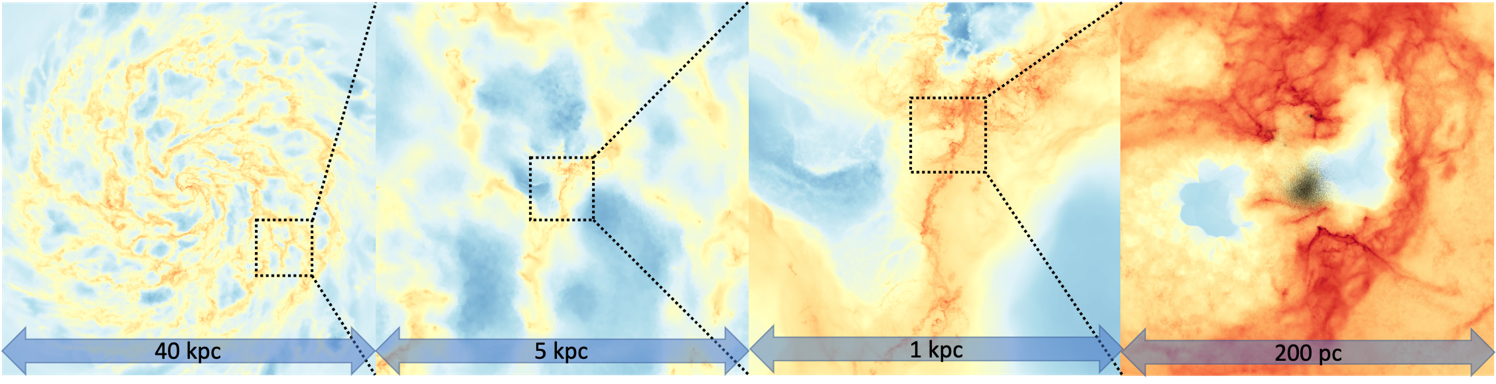
\includegraphics[width=\linewidth]{Outlook_img/Hui_sim.png}
    \caption{Gas surface density of a sequential zoom through a Milky Way-sized galaxy simulated using the moving-mesh code \texttt{Arepo}. The panels show: (1) a 40\,kpc face-on galactic disk; (2) a 5\,kpc local spiral structure; (3) one selected kpc-wide hyper-refinement region; and (4) a massive star-forming region centered at a star cluster (black dots). Credit: Hui Li.}
    \label{fig:hui-sim}
\end{figure}

\subsection{Applying machine-learning turbulence diagnostics beyond plasma simulations}
\fullsubsectionlabel{sec:awesom-beyond-plasma}

\begin{figure}[ht!]
    \centering
    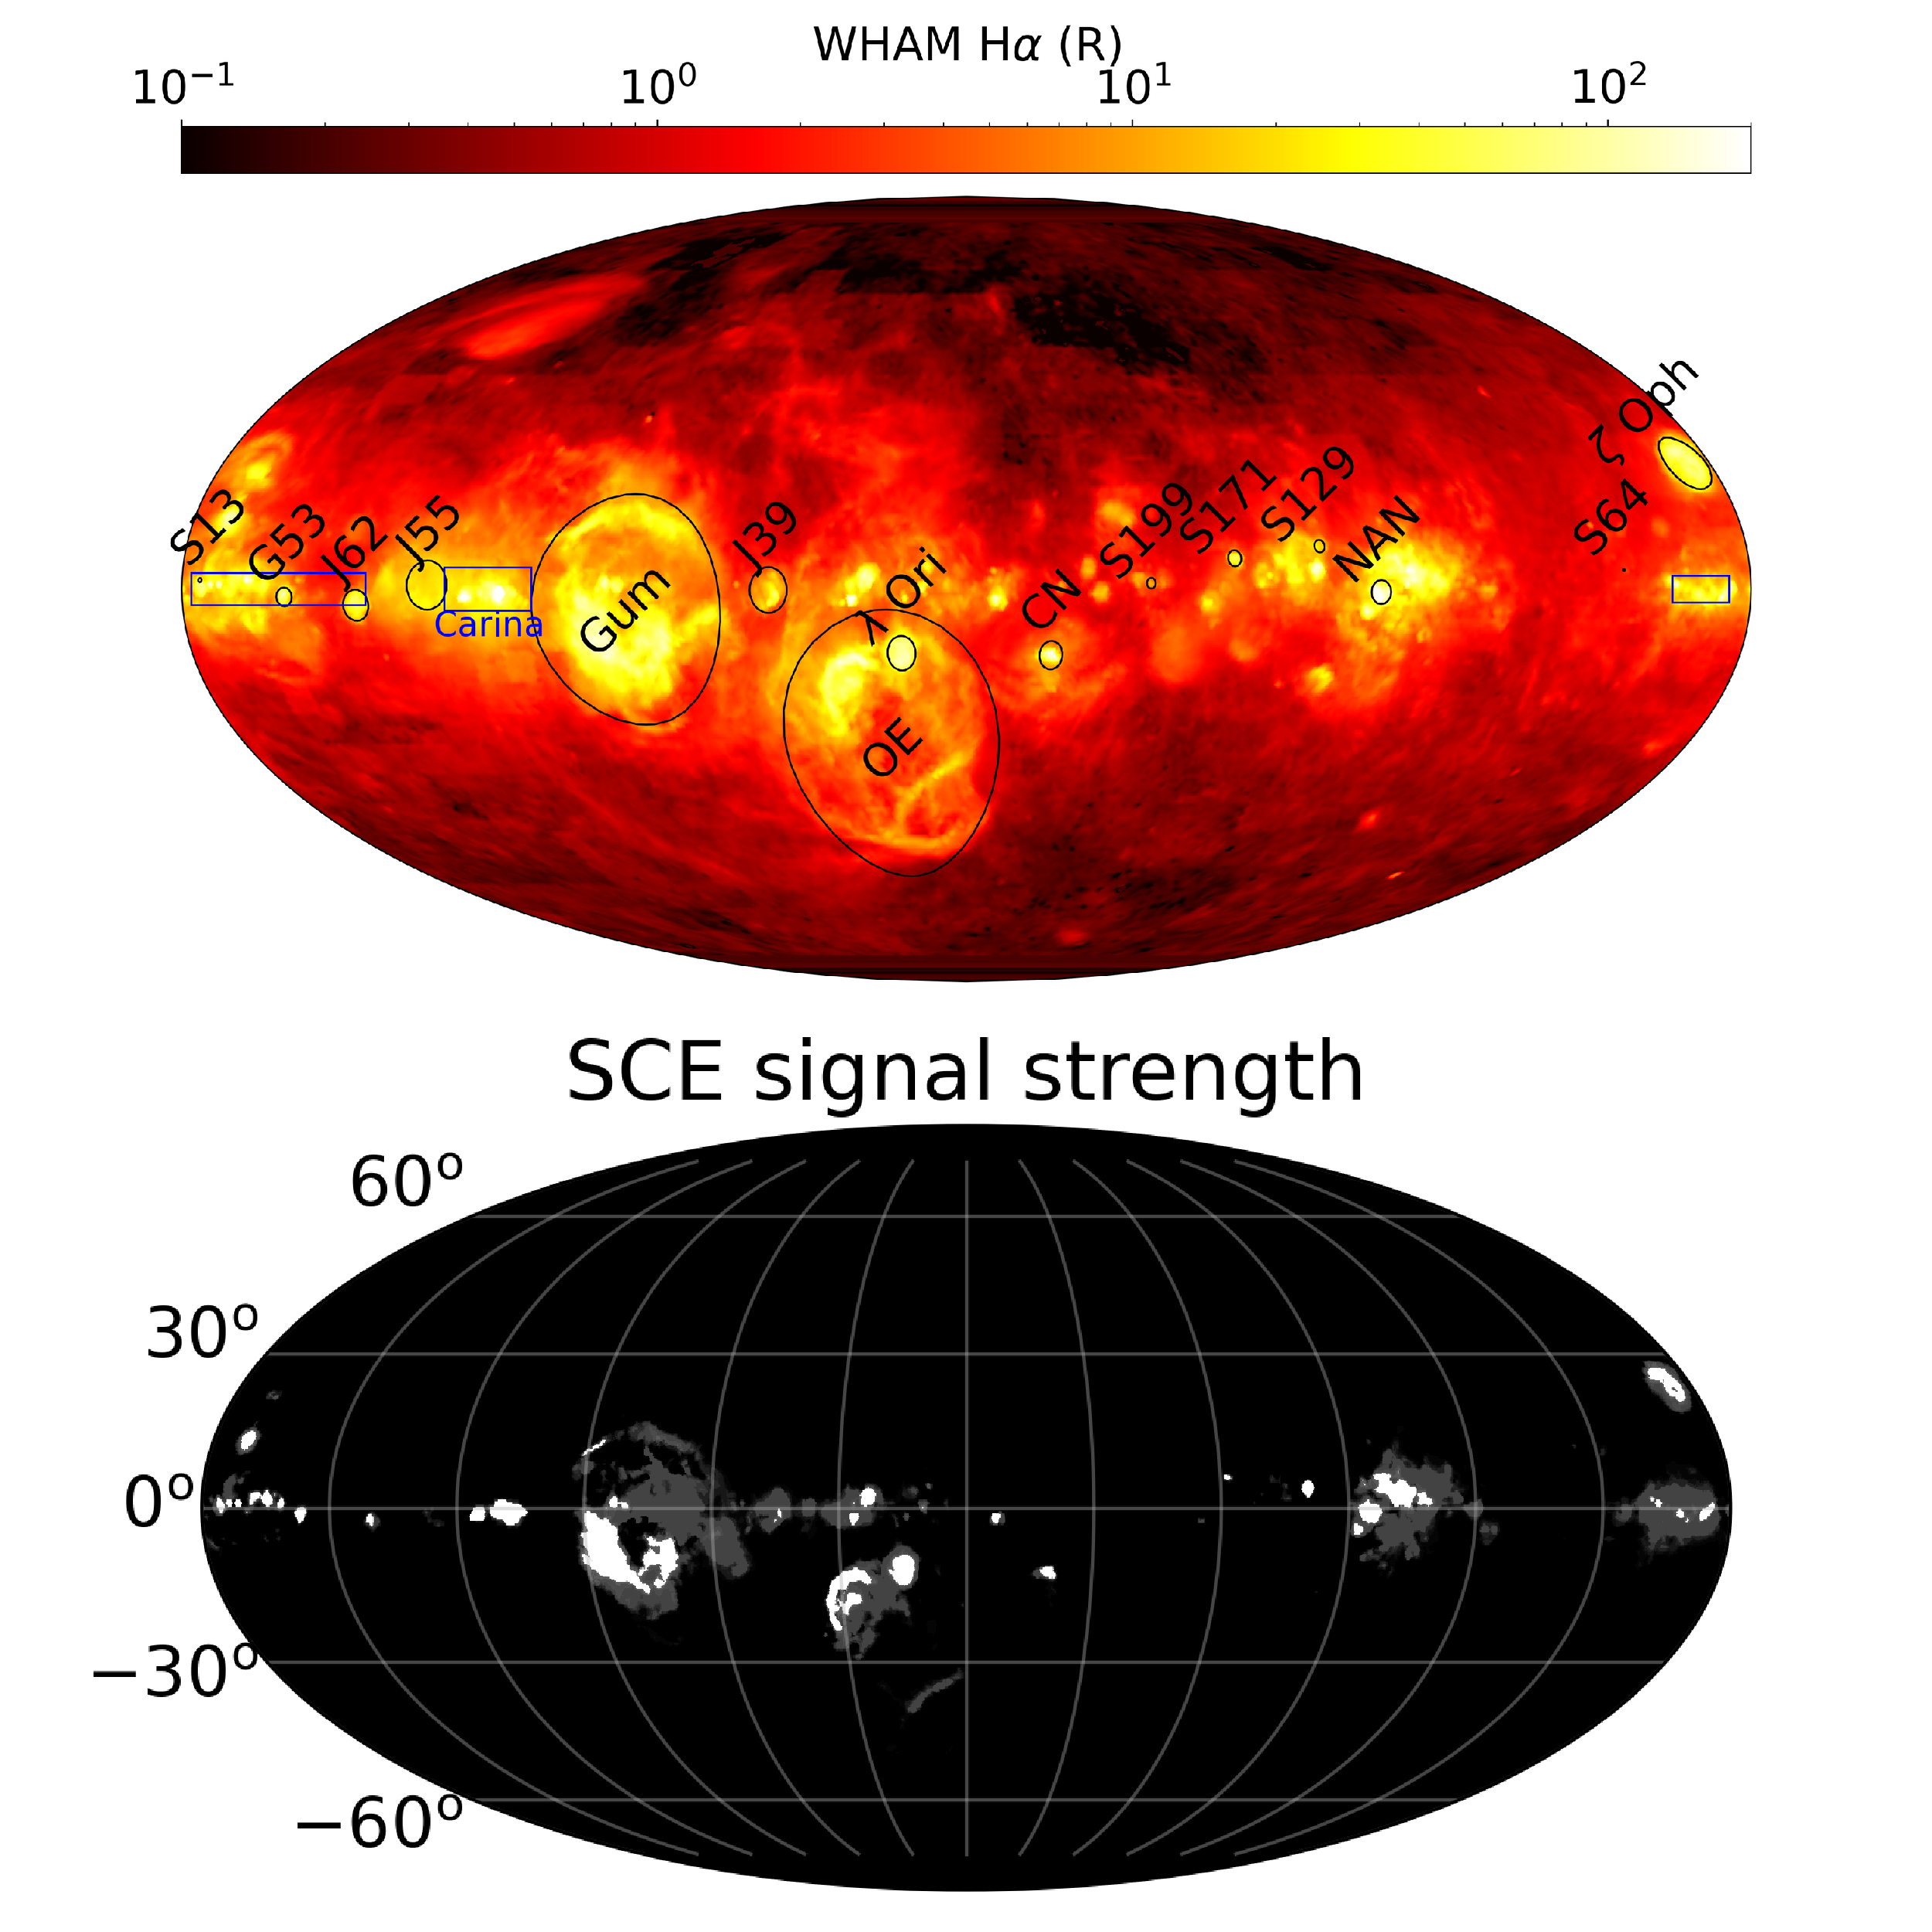
\includegraphics[width=\linewidth]{Outlook_img/SOM_Halpha.pdf}
    \caption{Preliminary application of \awesom\ to the all-sky Wisconsin H-Alpha Mapper (WHAM) \halpha\ survey \citep{haffner_wisconsin_2003}. Top: integrated \halpha\ intensity as a function of Galactic longitude and latitude, adapted from \citet{mccallum_halpha_2025}. Bottom: SCE signal strength obtained by combining multiple \awesom\ clustering realizations of the corresponding \halpha\ LOS velocity map. Regions of high SCE signal coincide with many star-forming regions and other prominent ionized structures, showing that the same unsupervised framework used for plasma-turbulence segmentation can also highlight coherent structures in observational ISM data.}
    \label{fig:som-halpha}
\end{figure}

Although \awesom\ was developed for plasma-turbulence segmentation, it can also be used for clustering or identification problems beyond the plasma domain.
As a demonstration, the online documentation\footnote{\url{https://awesom.readthedocs.io/en/latest/notebooks/iris.html}} applies the package to the Iris dataset \citep[][]{fisher_iris_1936}, a well-known non-linear classification problem.

An immediate extension of \awesom\ in the astronomy domain would be to apply the same unsupervised classification framework to high-dimensional observational maps, where the relevant structures are no longer current sheets but coherent regions of the multiphase ISM\@.
As an example, Figure~\ref{fig:som-halpha} shows an application to the WHAM survey, in which regions of high SCE signal in the \halpha\ LOS velocity data coincide with many star-forming regions and other prominent ionized structures.
This type of analysis can provide a data-driven method to define coherent ISM structures, such as star-forming regions or \ion{H}{2} regions, complementing existing rule-based methods.


\subsection{Connecting M87 simulations to X-ray velocity spectra}

\begin{figure}[t!]
    \centering
    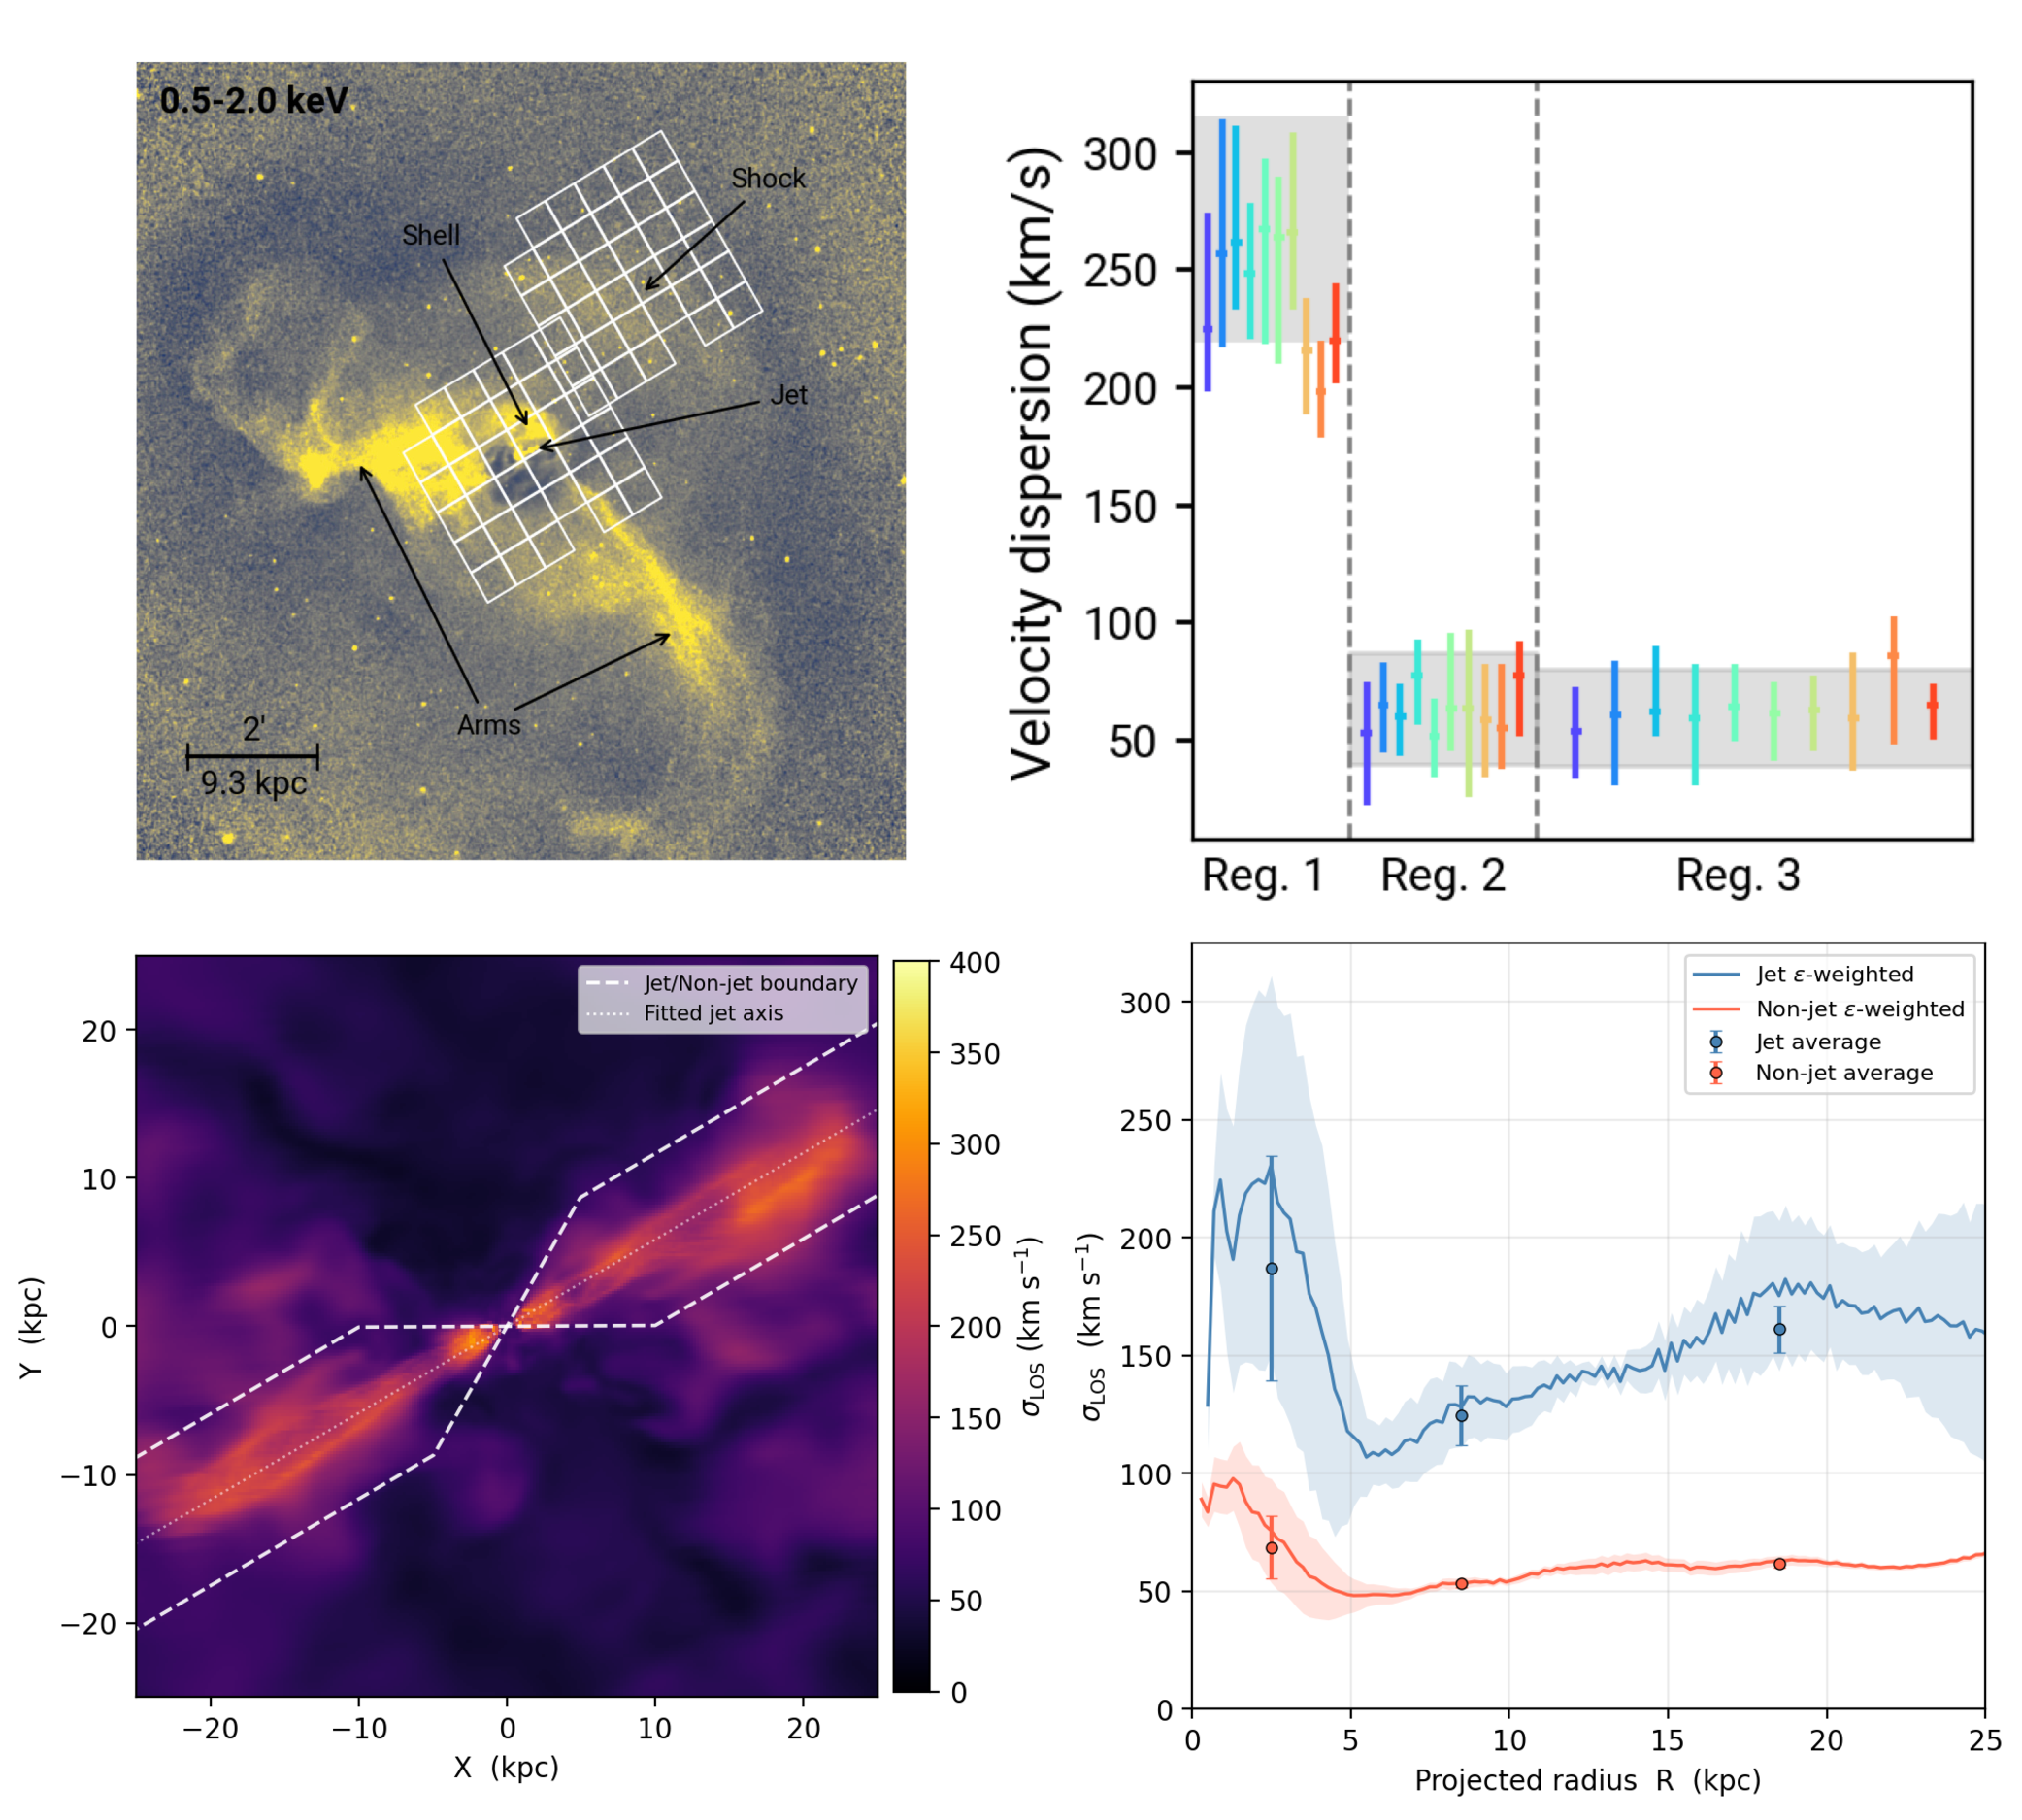
\includegraphics[width=\linewidth]{Outlook_img/Xray_los_sigma.pdf}
    \caption{Comparison between XRISM measurements of the M87 hot atmosphere and synthetic velocity dispersions from the simulations in Chapter~\ref{chap:sim}. Top left: \textit{Chandra} $0.5$--$2.0$\,keV image of the M87 core with the XRISM pointings overlaid, showing the jet, shell, shock front, and X-ray arms. Top right: XRISM (4.2 keV--7.0 keV band) LOS velocity dispersion in three projected radial regions, $0$--$5$\,kpc, $5$--$12$\,kpc, and $12$--$25$\,kpc. Images are adapted from \citet{xrism_collaboration_xrismresolve_2026}. Bottom left: simulated LOS velocity-dispersion map, with the dashed curves separating the jet and non-jet regions and the dotted line marking the projected jet axis. Bottom right: simulated radial profiles of the LOS velocity dispersion, $\sigma_{\rm LOS}$, in the jet and non-jet sectors, comparing unweighted and XRISM-band emissivity-weighted averages. This comparison makes the Chapter~\ref{chap:sim} simulation a direct benchmark against high-resolution observations in M87 \citep{ha_galaxy-_2026}.}
    \label{fig:xray-los-sigma}
\end{figure}

High-resolution X-ray spectroscopy now offers a direct observational benchmark for hot-gas velocity fields similar to those presented in Chapter~\ref{chap:sim}.
XRISM/Resolve recently measured LOS gas kinematics in the M87 atmosphere across three projected radial regions, finding a central velocity dispersion of $\sigma_{\rm LOS}=262^{+45}_{-38}\,\mathrm{km\,s^{-1}}$ within $0$--$5$\,kpc that then drops to $\sim 60\,\mathrm{km\,s^{-1}}$ from $5$--$25$\,kpc \citep{xrism_collaboration_xrismresolve_2026}.
This strong radial contrast highlights the central few kiloparsecs as the most turbulent region, where the AGN, jet, cavities, weak shocks, and X-ray shell coexist.
A direct comparison through mock observations also provides a more stringent target for simulations than density and temperature profiles alone, because the velocity dispersion directly constrains how mechanical energy is partitioned between coherent expansion, turbulent broadening, and bulk flows.

Figure~\ref{fig:xray-los-sigma} illustrates a preliminary comparison between the XRISM measurements and synthetic LOS velocity dispersions from the simulation in Chapter~\ref{chap:sim}.
The simulated maps show enhanced $\sigma_{\rm LOS}$ along the projected jet direction, while the non-jet regions are enhanced only in the central few kiloparsecs before plateauing at values similar to those measured by XRISM in the outskirts of the galaxy.
Further analysis with XRISM pointings along the jet and arms could test whether current jet prescriptions in galaxy simulations accurately model the kinetic-energy distribution of jet feedback.

\subsection{From meso-scale accretion to event-horizon GRMHD simulations}

One natural extension of Chapter~\ref{chap:sim} is to carry the meso-scale accretion flow all the way to the event horizon with GRMHD simulations.
Most horizon-scale simulations still initialize from ad hoc initial and boundary conditions, such as a torus of matter with an imposed poloidal or toroidal magnetic field.
Those setups have been useful for understanding generic black hole accretion, but they do not encode the multiphase morphology, angular momentum structure, or magnetic-field geometry produced by jet-driven turbulent mixing across galaxy-scale and meso-scale flows.
The next step in understanding multi-scale accretion in M87 is therefore to initialize event-horizon simulations directly from the gas distribution and magnetic-field geometry produced by meso-scale M87 simulations.

Such simulations would test how a realistic accretion morphology influences the flow around M87$^{\star}$, the launching of its jet, and the conditions required to build a magnetically arrested disk (MAD).
Adaptive mesh refinement can concentrate resolution near the disk and jet, allowing magnetic flux advection, jet power, and accretion variability to be followed in a setup that inherits structures from the larger-scale inflow.
The results enabled by these next-generation simulations would also create a more direct bridge to EHT observations: synthetic 230 GHz images and polarization maps from these simulations could be compared against existing M87$^{\star}$ observations and future time-dependent reconstructions of the black hole shadow.

The meso-scale simulations in Chapter~\ref{chap:sim} also show a warped accretion disk, with the angular momentum vector changing gradually with radius (see Figure~\ref{fig:main}).
If this warped disk is misaligned with the SMBH spin, Lense--Thirring precession should alter the inner disk orientation and may influence the direction of jet launching.
Future GRMHD simulations initialized from such warped inflows could therefore connect the angular momentum structure of the accreting gas to possible jet precession in M87, and test whether successive rings of misaligned gas can drive time-dependent changes in the jet nozzle direction.
In this way, the multi-scale approach developed in this dissertation can be extended from a model of black hole feeding to a model of the observable horizon-scale disk-jet system.

\begin{figure}[ht!]
    \centering
    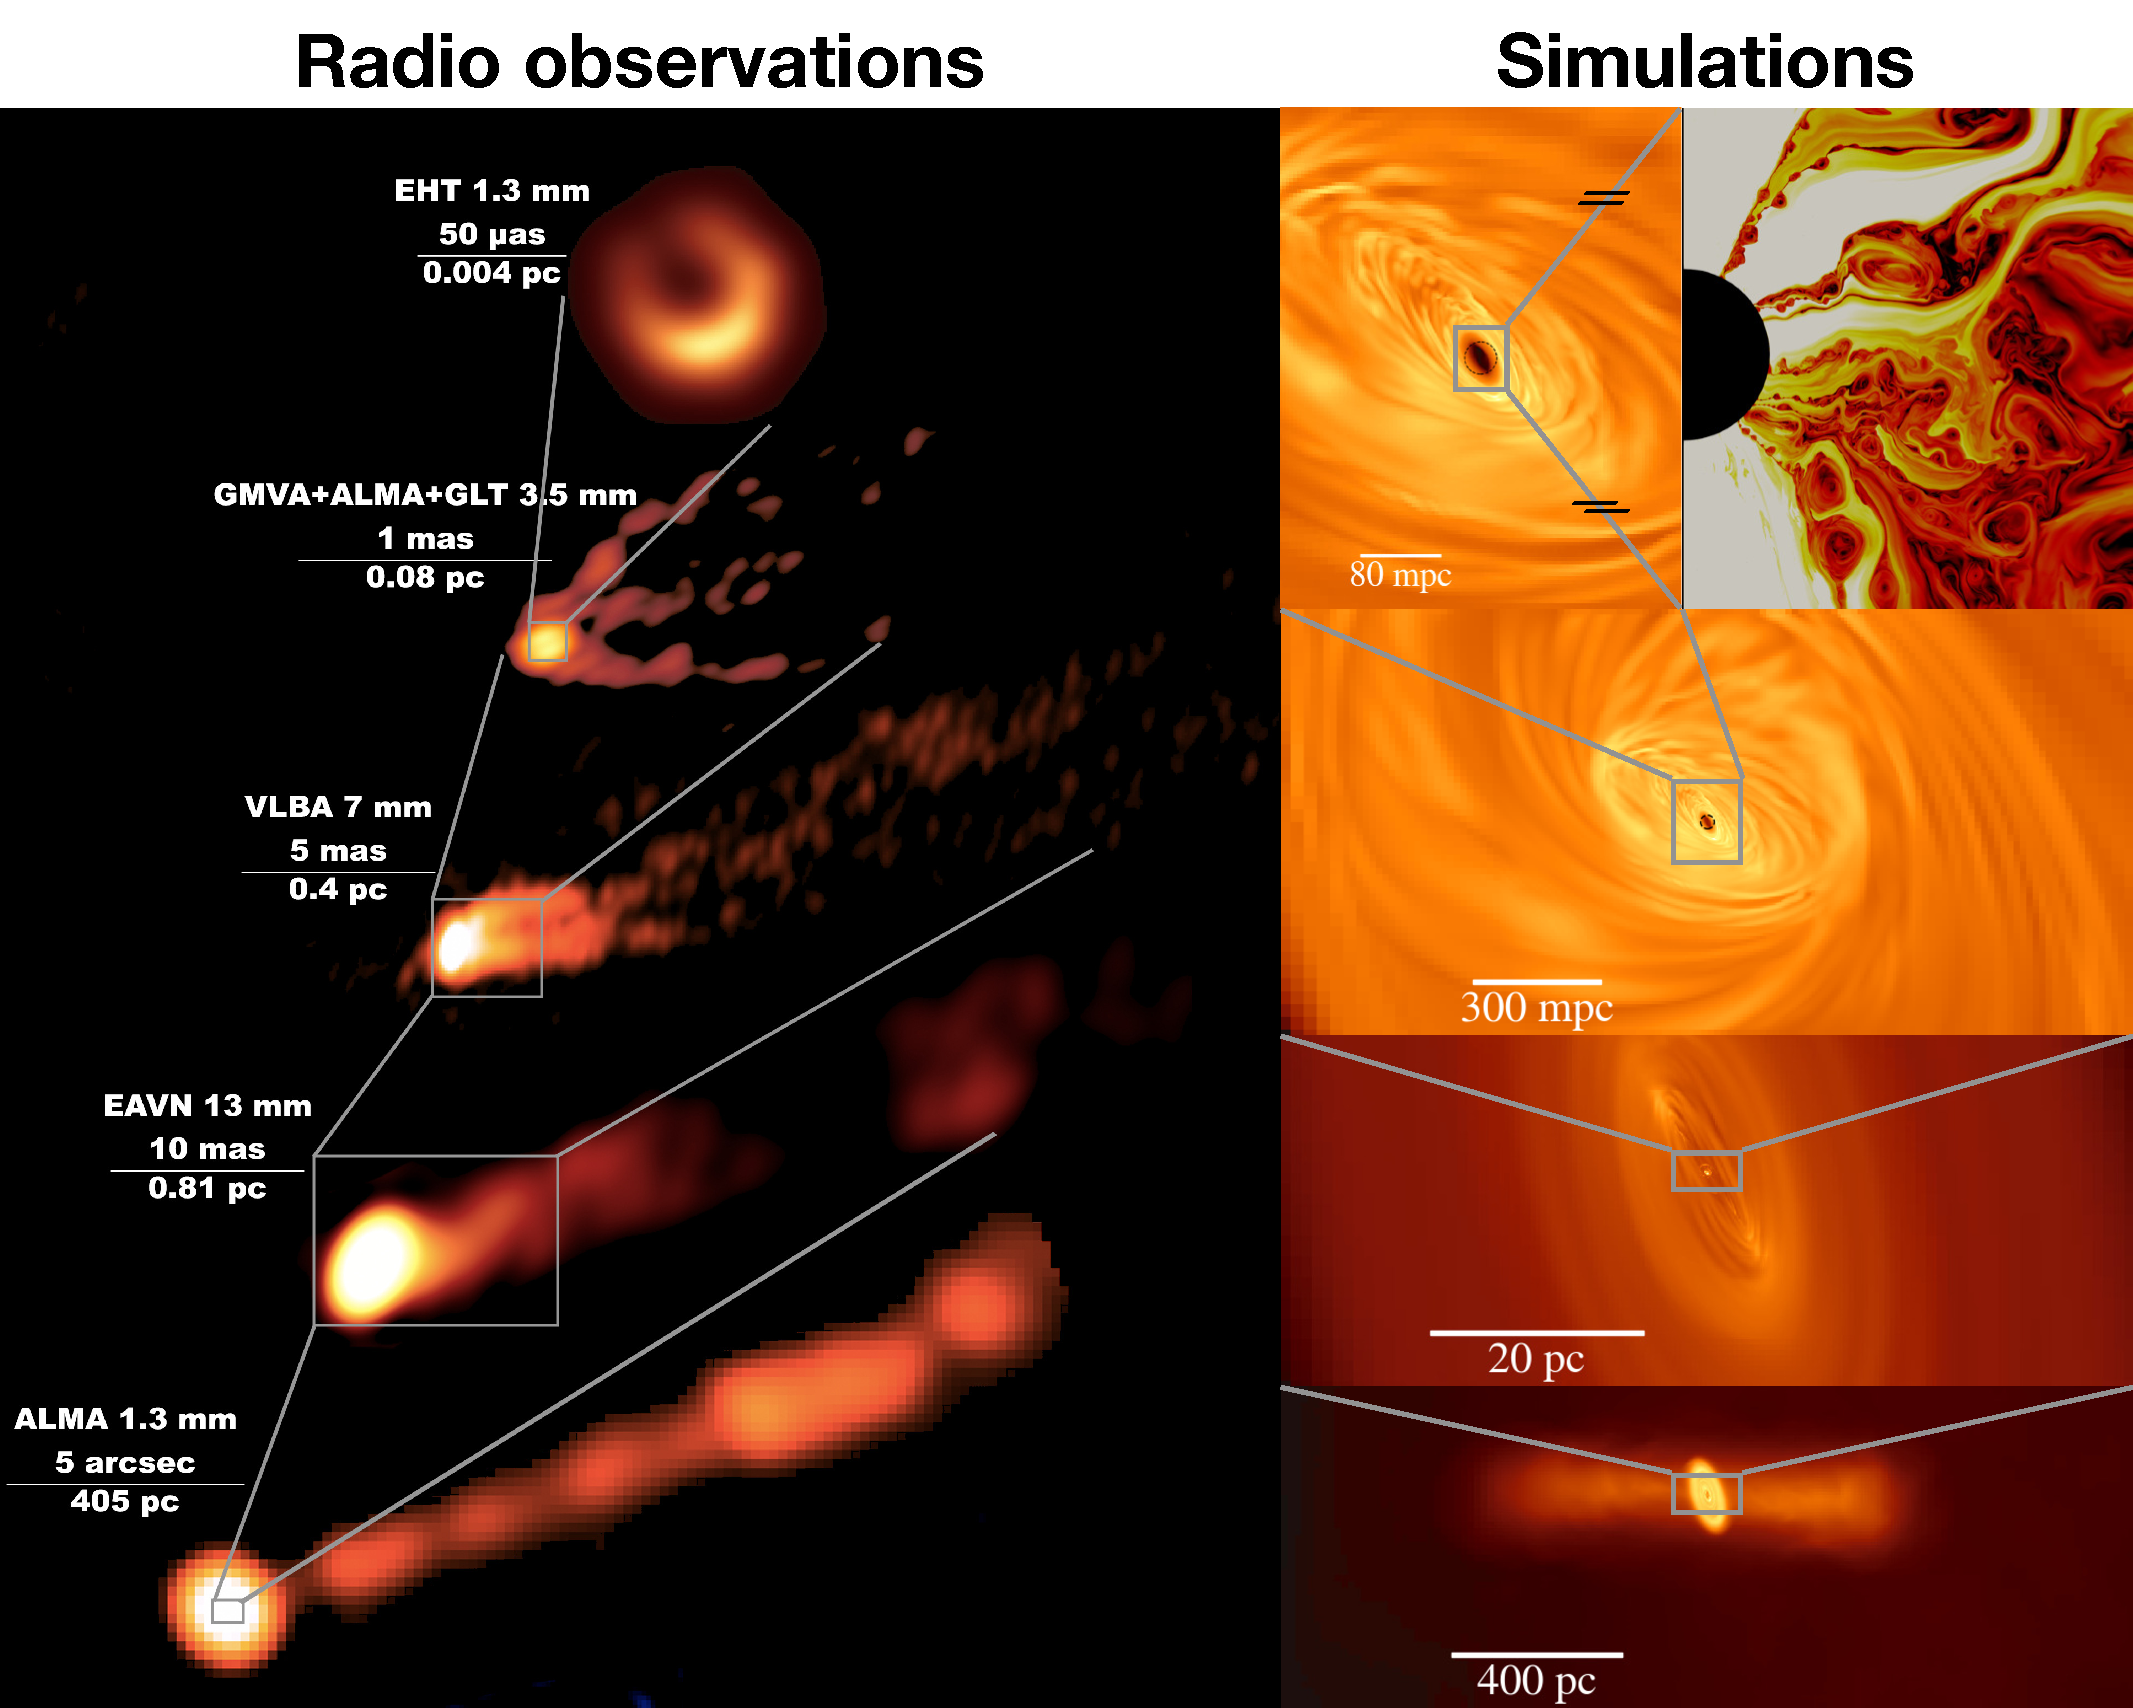
\includegraphics[width=\linewidth]{Outlook_img/obs-theory.pdf}
    \caption{The current state of modern observations and simulations in connecting a SMBH to its host galaxy. Left: observations of M87$^{\star}$, which resolve both the disk and the jet emission, adapted from \citet{algaba_broadband_2024}. Right: density projection plots from the multi-scale simulation presented in Chapter~\ref{chap:sim} \citep{ha_galaxy-_2026}. Window sizes range from $2$\,kpc to $0.5\,\mathrm{pc} \approx 10^3\,r_{\rm g}$ (gravitational radius). To understand the accretion process and multimessenger signals at the event-horizon scale (represented in the top right by a simulation of black hole accretion \citep{ripperda_magnetic_2020}), future GRMHD simulations can use initial conditions from this meso-scale accretion model.}
    \label{fig:main}
\end{figure}

\subsection{Reconnection, flares, and multimessenger signals}

The same event-horizon-scale simulations proposed in the previous subsection would also provide a path toward studying the high-energy signals produced by magnetic reconnection.
Bright TeV flares have been observed from M87 on timescales of several days, releasing a non-negligible fraction of the jet power during these events.
High-resolution GRMHD simulations suggest that these flares can be powered by reconnecting current sheets at several gravitational radii from the black hole, although the reconnection rate in ideal GRMHD simulations is often too slow to reproduce the observed variability \citep[e.g.,][]{ripperda_black_2022}.
Future work should therefore test whether more realistic accretion morphology, inherited magnetic-field structure, and effective resistivity prescriptions can reproduce reconnection-powered flares with both the correct energy spectra and timescales.

Another key challenge in accretion modeling is that magnetic reconnection events are still commonly identified and analyzed by hand.
This is manageable for a single prominent current sheet, but it becomes subjective and impractical when many reconnecting structures exist concurrently in a turbulent accretion flow.
The machine-learning framework developed in Chapter~\ref{chap:ml} provides a solution to make this measurement systematic: \awesom\ can be trained to identify reconnecting regions in GRMHD or PIC datasets, after which the spatial extent of each sheet can be used to measure inflow velocities, reconnection rates, and thermal dissipation profiles.
This would significantly accelerate efforts to understand current-sheet formation and energy dissipation through reconnection.

The same \awesom-based workflow also promises to enable modeling of reconnection-driven hadronic acceleration.
The source of ultra-high-energy cosmic rays (UHECRs) remains uncertain more than a century after their first detection, and recent IceCube observations of high-energy neutrinos from NGC 1068 have strengthened the case for particle acceleration in AGN environments \citep{collaboration_evidence_2022}.
In the corona region of AGNs, charged particles can meander between the two sides of a relativistic reconnection layer and gain energy during each crossing; similar acceleration may also occur in magnetically dominated turbulent regions near the equatorial current sheet, in flux tubes ejected during the MAD state, or along the jet boundary.
In future GRMHD simulations, test particles can be injected into the \awesom-identified reconnection layers to be followed through their acceleration and eventual escape from the simulation domain.
The energy spectrum of these particles would test whether low-luminosity AGNs such as M87$^{\star}$ can accelerate UHECR particles that later produce observable multimessenger signals.

A further extension of this analysis would integrate \awesom\ directly into GRMHD simulations as a runtime detector for reconnection events.
When the detector identifies a reconnecting layer, test particles could be injected at the site and followed until they leave the domain.
This approach would reduce the number of particles tracked throughout the full simulation and would also reduce the need to store dense restart outputs for post-processing.
The resulting particle spectra could then test whether the accretion flow around M87$^{\star}$ can produce UHECRs or high-energy neutrinos.

\section{Concluding Remarks}

Stellar kinematic surveys, kinetic plasma simulations, X-ray spectroscopy, and event-horizon modeling now constrain turbulence across physical scales from molecular clouds to black hole accretion flows.
Across these regimes, turbulence is becoming less an obscure signal inferred indirectly and more a measurable, well-constrained physical process that regulates star formation, plasma heating, black hole feeding, and feedback.
This dissertation has developed three complementary routes for constraining astrophysical turbulence: stellar velocity statistics for measuring turbulence in molecular clouds, machine-learning methods for identifying intermittent structures in relativistic plasma, and multi-scale simulations for connecting SMBH feeding to jet feedback in M87.



%------------------------------------------------------------------
% BIBLIOGRAPHY INFORMATION
\newpage
\addtocontents{toc}{\hfill \par}
\phantomsection
\addcontentsline{toc}{chapter}{\hspace{1em}\bibname}
%------------------------------------------------------------------------------------

\begingroup
\singlespacing
\setlength{\bibsep}{1.00\baselineskip}   % double-spaced between entries
\interlinepenalty=10000                   % keep each entry on a single page
\bibliographystyle{aasjournal}
\bibliography{references}
\endgroup

% \bibliographystyle{aasjournal}   %Can change the style of your bibliography
% \bibliography{references}      %Enter your bib file's name here

\end{document}
